% Customizable fields and text areas start with % >> below.
% Lines starting with the comment character (%) are normally removed before release outside the collaboration, but not those comments ending lines

% svn info. These are modified by svn at checkout time.
% The last version of these macros found before the maketitle will be the one on the front page,
% so only the main file is tracked.
% Do not edit by hand!
\RCS$Revision: 95458 $
\RCS$HeadURL: file:///afs/cern.ch/project/svn/reps/tdr2/notes/AN-11-417/trunk/AN-11-417.tex $
\RCS$Id: AN-11-417.tex 95458 2012-01-16 15:38:04Z hwoehri $
%%%%%%%%%%%%% ptdr definitions %%%%%%%%%%%%%%%%%%%%%
%%%%%%%%%%%%%%%%%%%%%%%%%%%%%%%%%%%%%%%%%%%%%%%%%%%%%%%%%%%%%%%%%%%%%
%
%  Common definitions
%
%  N.B. use of \providecommand rather than \newcommand means
%       that a definition is ignored if already specified
%
%                                              L. Taylor 18 Feb 2005
%%%%%%%%%%%%%%%%%%%%%%%%%%%%%%%%%%%%%%%%%%%%%%%%%%%%%%%%%%%%%%%%%%%%

% Some shorthand
% turn off italics
\newcommand {\etal}{\mbox{et al.}\xspace} %et al. - no preceding comma
\newcommand {\ie}{\mbox{i.e.}\xspace}     %i.e.
\newcommand {\eg}{\mbox{e.g.}\xspace}     %e.g.
\newcommand {\etc}{\mbox{etc.}\xspace}     %etc.
\newcommand {\vs}{\mbox{\sl vs.}\xspace}      %vs.
\newcommand {\mdash}{\ensuremath{\mathrm{-}}} % for use within formulas

% some terms whose definition we may change
\newcommand {\Lone}{Level-1\xspace} % Level-1 or L1 ?
\newcommand {\Ltwo}{Level-2\xspace}
\newcommand {\Lthree}{Level-3\xspace}

% Some software programs (alphabetized)
\providecommand{\ACERMC} {\textsc{AcerMC}\xspace}
\providecommand{\ALPGEN} {{\textsc{alpgen}}\xspace}
\providecommand{\CHARYBDIS} {{\textsc{charybdis}}\xspace}
\providecommand{\CMKIN} {\textsc{cmkin}\xspace}
\providecommand{\CMSIM} {{\textsc{cmsim}}\xspace}
\providecommand{\CMSSW} {{\textsc{cmssw}}\xspace}
\providecommand{\COBRA} {{\textsc{cobra}}\xspace}
\providecommand{\COCOA} {{\textsc{cocoa}}\xspace}
\providecommand{\COMPHEP} {\textsc{CompHEP}\xspace}
\providecommand{\EVTGEN} {{\textsc{evtgen}}\xspace}
\providecommand{\FAMOS} {{\textsc{famos}}\xspace}
\providecommand{\GARCON} {\textsc{garcon}\xspace}
\providecommand{\GARFIELD} {{\textsc{garfield}}\xspace}
\providecommand{\GEANE} {{\textsc{geane}}\xspace}
\providecommand{\GEANTfour} {{\textsc{geant4}}\xspace}
\providecommand{\GEANTthree} {{\textsc{geant3}}\xspace}
\providecommand{\GEANT} {{\textsc{geant}}\xspace}
\providecommand{\HDECAY} {\textsc{hdecay}\xspace}
\providecommand{\HERWIG} {{\textsc{herwig}}\xspace}
\providecommand{\HIGLU} {{\textsc{higlu}}\xspace}
\providecommand{\HIJING} {{\textsc{hijing}}\xspace}
\providecommand{\IGUANA} {\textsc{iguana}\xspace}
\providecommand{\ISAJET} {{\textsc{isajet}}\xspace}
\providecommand{\ISAPYTHIA} {{\textsc{isapythia}}\xspace}
\providecommand{\ISASUGRA} {{\textsc{isasugra}}\xspace}
\providecommand{\ISASUSY} {{\textsc{isasusy}}\xspace}
\providecommand{\ISAWIG} {{\textsc{isawig}}\xspace}
\providecommand{\MADGRAPH} {\textsc{MadGraph}\xspace}
\providecommand{\MCATNLO} {\textsc{mc@nlo}\xspace}
\providecommand{\MCFM} {\textsc{mcfm}\xspace}
\providecommand{\MILLEPEDE} {{\textsc{millepede}}\xspace}
\providecommand{\ORCA} {{\textsc{orca}}\xspace}
\providecommand{\OSCAR} {{\textsc{oscar}}\xspace}
\providecommand{\PHOTOS} {\textsc{photos}\xspace}
\providecommand{\PROSPINO} {\textsc{prospino}\xspace}
\providecommand{\PYTHIA} {{\textsc{pythia}}\xspace}
\providecommand{\SHERPA} {{\textsc{sherpa}}\xspace}
\providecommand{\TAUOLA} {\textsc{tauola}\xspace}
\providecommand{\TOPREX} {\textsc{TopReX}\xspace}
\providecommand{\XDAQ} {{\textsc{xdaq}}\xspace}


%  Experiments
\newcommand {\DZERO}{D\O\xspace}     %etc.


% Measurements and units...

\newcommand{\de}{\ensuremath{^\circ}}
\newcommand{\ten}[1]{\ensuremath{\times \text{10}^\text{#1}}}
\newcommand{\unit}[1]{\ensuremath{\text{\,#1}}\xspace}
\newcommand{\mum}{\ensuremath{\,\mu\text{m}}\xspace}
\newcommand{\micron}{\ensuremath{\,\mu\text{m}}\xspace}
\newcommand{\cm}{\ensuremath{\,\text{cm}}\xspace}
\newcommand{\mm}{\ensuremath{\,\text{mm}}\xspace}
\newcommand{\mus}{\ensuremath{\,\mu\text{s}}\xspace}
\newcommand{\keV}{\ensuremath{\,\text{ke\hspace{-.08em}V}}\xspace}
\newcommand{\MeV}{\ensuremath{\,\text{Me\hspace{-.08em}V}}\xspace}
\newcommand{\GeV}{\ensuremath{\,\text{Ge\hspace{-.08em}V}}\xspace}
\newcommand{\TeV}{\ensuremath{\,\text{Te\hspace{-.08em}V}}\xspace}
\newcommand{\PeV}{\ensuremath{\,\text{Pe\hspace{-.08em}V}}\xspace}
\newcommand{\keVc}{\ensuremath{{\,\text{ke\hspace{-.08em}V\hspace{-0.16em}/\hspace{-0.08em}}c}}\xspace}
\newcommand{\MeVc}{\ensuremath{{\,\text{Me\hspace{-.08em}V\hspace{-0.16em}/\hspace{-0.08em}}c}}\xspace}
\newcommand{\GeVc}{\ensuremath{{\,\text{Ge\hspace{-.08em}V\hspace{-0.16em}/\hspace{-0.08em}}c}}\xspace}
\newcommand{\TeVc}{\ensuremath{{\,\text{Te\hspace{-.08em}V\hspace{-0.16em}/\hspace{-0.08em}}c}}\xspace}
\newcommand{\keVcc}{\ensuremath{{\,\text{ke\hspace{-.08em}V\hspace{-0.16em}/\hspace{-0.08em}}c^\text{2}}}\xspace}
\newcommand{\MeVcc}{\ensuremath{{\,\text{Me\hspace{-.08em}V\hspace{-0.16em}/\hspace{-0.08em}}c^\text{2}}}\xspace}
\newcommand{\GeVcc}{\ensuremath{{\,\text{Ge\hspace{-.08em}V\hspace{-0.16em}/\hspace{-0.08em}}c^\text{2}}}\xspace}
\newcommand{\TeVcc}{\ensuremath{{\,\text{Te\hspace{-.08em}V\hspace{-0.16em}/\hspace{-0.08em}}c^\text{2}}}\xspace}

\newcommand{\pbinv} {\mbox{\ensuremath{\,\text{pb}^\text{$-$1}}}\xspace}
\newcommand{\fbinv} {\mbox{\ensuremath{\,\text{fb}^\text{$-$1}}}\xspace}
\newcommand{\nbinv} {\mbox{\ensuremath{\,\text{nb}^\text{$-$1}}}\xspace}
\newcommand{\percms}{\ensuremath{\,\text{cm}^\text{$-$2}\,\text{s}^\text{$-$1}}\xspace}
\newcommand{\lumi}{\ensuremath{\mathcal{L}}\xspace}
\newcommand{\Lumi}{\ensuremath{\mathcal{L}}\xspace}%both upper and lower
%
% Need a convention here:
\newcommand{\LvLow}  {\ensuremath{\mathcal{L}=\text{10}^\text{32}\,\text{cm}^\text{$-$2}\,\text{s}^\text{$-$1}}\xspace}
\newcommand{\LLow}   {\ensuremath{\mathcal{L}=\text{10}^\text{33}\,\text{cm}^\text{$-$2}\,\text{s}^\text{$-$1}}\xspace}
\newcommand{\lowlumi}{\ensuremath{\mathcal{L}=\text{2}\times \text{10}^\text{33}\,\text{cm}^\text{$-$2}\,\text{s}^\text{$-$1}}\xspace}
\newcommand{\LMed}   {\ensuremath{\mathcal{L}=\text{2}\times \text{10}^\text{33}\,\text{cm}^\text{$-$2}\,\text{s}^\text{$-$1}}\xspace}
\newcommand{\LHigh}  {\ensuremath{\mathcal{L}=\text{10}^\text{34}\,\text{cm}^\text{$-$2}\,\text{s}^\text{$-$1}}\xspace}
\newcommand{\hilumi} {\ensuremath{\mathcal{L}=\text{10}^\text{34}\,\text{cm}^\text{$-$2}\,\text{s}^\text{$-$1}}\xspace}

% Some usual physics terms


% SM (still to be classified)

\newcommand{\kt}{\ensuremath{k_{\mathrm{T}}}\xspace}
\newcommand{\BC}{\ensuremath{{B_{\mathrm{c}}}}\xspace}
\newcommand{\bbarc}{\ensuremath{{\overline{b}c}}\xspace}
\newcommand{\bbbar}{\ensuremath{{b\overline{b}}}\xspace}
\newcommand{\ccbar}{\ensuremath{{c\overline{c}}}\xspace}
\newcommand{\JPsi}{\ensuremath{{J}\hspace{-.08em}/\hspace{-.14em}\psi}\xspace}
\newcommand{\bspsiphi}{\ensuremath{B_s \to \JPsi\, \phi}\xspace}
%\newcommand{\ttbar}{\ensuremath{{t\overline{t}}}\xspace}
\newcommand{\AFB}{\ensuremath{A_\text{FB}}\xspace}
\newcommand{\EE}{\ensuremath{e^+e^-}\xspace}
\newcommand{\MM}{\ensuremath{\mu^+\mu^-}\xspace}
\newcommand{\TT}{\ensuremath{\tau^+\tau^-}\xspace}
\newcommand{\wangle}{\ensuremath{\sin^{2}\theta_{\text{eff}}^\text{lept}(M^2_\mathrm{Z})}\xspace}
\newcommand{\ttbar}{\ensuremath{{t\overline{t}}}\xspace}
\newcommand{\stat}{\ensuremath{\,\text{(stat.)}}\xspace}
\newcommand{\syst}{\ensuremath{\,\text{(syst.)}}\xspace}
% these moved to similar defs
%\newcommand{\Etmiss}{\ensuremath{E_{\mathrm{T}\!{\rm miss}}}}
%\newcommand{\VEtmiss}{\ensuremath{{\vec E}_{\mathrm{T}\!{\rm miss}}}}

%%%  E-gamma definitions
\newcommand{\HGG}{\ensuremath{\mathrm{H}\to\gamma\gamma}}
\newcommand{\gev}{\GeV}
\newcommand{\GAMJET}{\ensuremath{\gamma + \text{jet}}}
\newcommand{\PPTOJETS}{\ensuremath{\mathrm{pp}\to\text{jets}}}
\newcommand{\PPTOGG}{\ensuremath{\mathrm{pp}\to\gamma\gamma}}
\newcommand{\PPTOGAMJET}{\ensuremath{\mathrm{pp}\to\gamma +
\mathrm{jet}
}}
\newcommand{\MH}{\ensuremath{\mathrm{M_{\mathrm{H}}}}}
\newcommand{\RNINE}{\ensuremath{\mathrm{R}_\mathrm{9}}}
\newcommand{\DR}{\ensuremath{\Delta\mathrm{R}}}



% Physics symbols ...

\newcommand{\PT}{\ensuremath{p_{\mathrm{T}}}\xspace}
\newcommand{\pt}{\ensuremath{p_{\mathrm{T}}}\xspace}
\newcommand{\ET}{\ensuremath{E_{\mathrm{T}}}\xspace}
\newcommand{\HT}{\ensuremath{H_{\mathrm{T}}}\xspace}
\newcommand{\et}{\ensuremath{E_{\mathrm{T}}}\xspace}
\providecommand{\Em}{\ensuremath{E\hspace{-0.6em}/}\xspace}
\providecommand{\Pm}{\ensuremath{p\hspace{-0.5em}/}\xspace}
\providecommand{\PTm}{\ensuremath{{p}_\mathrm{T}\hspace{-1.02em}/}\xspace}
\providecommand{\PTslash}{\ensuremath{{p}_\mathrm{T}\hspace{-1.02em}/}\xspace}
\newcommand{\ETm}{\ensuremath{E_{\mathrm{T}}^{\text{miss}}}\xspace}
\providecommand{\ETslash}{\ensuremath{E_{\mathrm{T}}\hspace{-1.1em}/}\xspace}
\newcommand{\MET}{\ensuremath{E_{\mathrm{T}}^{\text{miss}}}\xspace}
\newcommand{\ETmiss}{\ensuremath{E_{\mathrm{T}}^{\text{miss}}}\xspace}
\newcommand{\VEtmiss}{\ensuremath{{\vec E}_{\mathrm{T}}^{\text{miss}}}\xspace}

% roman face derivative
\providecommand{\dd}[2]{\ensuremath{\frac{\mathrm{d} #1}{\mathrm{d} #2}}}
% Particle names which will track the italic/non-italic face convention
\providecommand{\zp}{\ensuremath{\mathrm{Z}^\prime}\xspace}
\providecommand{\JPsi}{\ensuremath{\mathrm{J}\hspace{-.08em}/\hspace{-.14em}\psi}\xspace}
\providecommand{\Z}{\ensuremath{\mathrm{Z}}\xspace}
\providecommand{\ttbar}{\ensuremath{\mathrm{t}\overline{\mathrm{t}}}\xspace}
% Extensions for missing names in PENNAMES
\providecommand{\cPgn}{\ensuremath{\nu}\xspace} % generic neutrino
\providecommand{\cPJgy}{\JPsi} % J/Psi (no mass)
\providecommand{\cPZ}{\Z} % plain Z (no superscript 0)
\providecommand{\cPZpr}{\zp} % plain Z'
% SymbolFace not yet available in trunk version
%\providecommand{\cPqb}{\ensuremath{\cmsSymbolFace{b}}\xspace} % b for b quark
%\providecommand{\cPqt}{\ensuremath{\cmsSymbolFace{t}}\xspace} % t for t quark
%\providecommand{\cPqc}{\ensuremath{\cmsSymbolFace{c}}\xspace} % c for c quark
%\providecommand{\cPaqb}{\ensuremath{\overline{\cmsSymbolFace{b}}\xspace}} % b for b anti-quark
%\providecommand{\cPaqt}{\ensuremath{\overline{\cmsSymbolFace{t}}}\xspace} % t for t anti-quark
%\providecommand{\cPaqc}{\ensuremath{\overline{\cmsSymbolFace{c}}}\xspace} % c for c anti-quark
%%%%%%
% From Albert
%

\newcommand{\ga}{\ensuremath{\gtrsim}}
\newcommand{\la}{\ensuremath{\lesssim}}
%\def\ga{\mathrel{\rlap{\raise.6ex\hbox{$>$}}{\lower.6ex\hbox{$\sim$}}}}
%\def\la{\mathrel{\rlap{\raise.6ex\hbox{$<$}}{\lower.6ex\hbox{$\sim$}}}}
%
\newcommand{\swsq}{\ensuremath{\sin^2\theta_W}\xspace}
\newcommand{\cwsq}{\ensuremath{\cos^2\theta_W}\xspace}
\newcommand{\tanb}{\ensuremath{\tan\beta}\xspace}
\newcommand{\tanbsq}{\ensuremath{\tan^{2}\beta}\xspace}
\newcommand{\sidb}{\ensuremath{\sin 2\beta}\xspace}
\newcommand{\alpS}{\ensuremath{\alpha_S}\xspace}
\newcommand{\alpt}{\ensuremath{\tilde{\alpha}}\xspace}

\newcommand{\QL}{\ensuremath{Q_L}\xspace}
\newcommand{\sQ}{\ensuremath{\tilde{Q}}\xspace}
\newcommand{\sQL}{\ensuremath{\tilde{Q}_L}\xspace}
\newcommand{\ULC}{\ensuremath{U_L^C}\xspace}
\newcommand{\sUC}{\ensuremath{\tilde{U}^C}\xspace}
\newcommand{\sULC}{\ensuremath{\tilde{U}_L^C}\xspace}
\newcommand{\DLC}{\ensuremath{D_L^C}\xspace}
\newcommand{\sDC}{\ensuremath{\tilde{D}^C}\xspace}
\newcommand{\sDLC}{\ensuremath{\tilde{D}_L^C}\xspace}
\newcommand{\LL}{\ensuremath{L_L}\xspace}
\newcommand{\sL}{\ensuremath{\tilde{L}}\xspace}
\newcommand{\sLL}{\ensuremath{\tilde{L}_L}\xspace}
\newcommand{\ELC}{\ensuremath{E_L^C}\xspace}
\newcommand{\sEC}{\ensuremath{\tilde{E}^C}\xspace}
\newcommand{\sELC}{\ensuremath{\tilde{E}_L^C}\xspace}
\newcommand{\sEL}{\ensuremath{\tilde{E}_L}\xspace}
\newcommand{\sER}{\ensuremath{\tilde{E}_R}\xspace}
\newcommand{\sFer}{\ensuremath{\tilde{f}}\xspace}
\newcommand{\sQua}{\ensuremath{\tilde{q}}\xspace}
\newcommand{\sUp}{\ensuremath{\tilde{u}}\xspace}
\newcommand{\suL}{\ensuremath{\tilde{u}_L}\xspace}
\newcommand{\suR}{\ensuremath{\tilde{u}_R}\xspace}
\newcommand{\sDw}{\ensuremath{\tilde{d}}\xspace}
\newcommand{\sdL}{\ensuremath{\tilde{d}_L}\xspace}
\newcommand{\sdR}{\ensuremath{\tilde{d}_R}\xspace}
\newcommand{\sTop}{\ensuremath{\tilde{t}}\xspace}
\newcommand{\stL}{\ensuremath{\tilde{t}_L}\xspace}
\newcommand{\stR}{\ensuremath{\tilde{t}_R}\xspace}
\newcommand{\stone}{\ensuremath{\tilde{t}_1}\xspace}
\newcommand{\sttwo}{\ensuremath{\tilde{t}_2}\xspace}
\newcommand{\sBot}{\ensuremath{\tilde{b}}\xspace}
\newcommand{\sbL}{\ensuremath{\tilde{b}_L}\xspace}
\newcommand{\sbR}{\ensuremath{\tilde{b}_R}\xspace}
\newcommand{\sbone}{\ensuremath{\tilde{b}_1}\xspace}
\newcommand{\sbtwo}{\ensuremath{\tilde{b}_2}\xspace}
\newcommand{\sLep}{\ensuremath{\tilde{l}}\xspace}
\newcommand{\sLepC}{\ensuremath{\tilde{l}^C}\xspace}
\newcommand{\sEl}{\ensuremath{\tilde{e}}\xspace}
\newcommand{\sElC}{\ensuremath{\tilde{e}^C}\xspace}
\newcommand{\seL}{\ensuremath{\tilde{e}_L}\xspace}
\newcommand{\seR}{\ensuremath{\tilde{e}_R}\xspace}
\newcommand{\snL}{\ensuremath{\tilde{\nu}_L}\xspace}
\newcommand{\sMu}{\ensuremath{\tilde{\mu}}\xspace}
\newcommand{\sNu}{\ensuremath{\tilde{\nu}}\xspace}
\newcommand{\sTau}{\ensuremath{\tilde{\tau}}\xspace}
\newcommand{\Glu}{\ensuremath{g}\xspace}
\newcommand{\sGlu}{\ensuremath{\tilde{g}}\xspace}
\newcommand{\Wpm}{\ensuremath{W^{\pm}}\xspace}
\newcommand{\sWpm}{\ensuremath{\tilde{W}^{\pm}}\xspace}
\newcommand{\Wz}{\ensuremath{W^{0}}\xspace}
\newcommand{\sWz}{\ensuremath{\tilde{W}^{0}}\xspace}
\newcommand{\sWino}{\ensuremath{\tilde{W}}\xspace}
\newcommand{\Bz}{\ensuremath{B^{0}}\xspace}
\newcommand{\sBz}{\ensuremath{\tilde{B}^{0}}\xspace}
\newcommand{\sBino}{\ensuremath{\tilde{B}}\xspace}
\newcommand{\Zz}{\ensuremath{Z^{0}}\xspace}
\newcommand{\sZino}{\ensuremath{\tilde{Z}^{0}}\xspace}
\newcommand{\sGam}{\ensuremath{\tilde{\gamma}}\xspace}
\newcommand{\chiz}{\ensuremath{\tilde{\chi}^{0}}\xspace}
\newcommand{\chip}{\ensuremath{\tilde{\chi}^{+}}\xspace}
\newcommand{\chim}{\ensuremath{\tilde{\chi}^{-}}\xspace}
\newcommand{\chipm}{\ensuremath{\tilde{\chi}^{\pm}}\xspace}
\newcommand{\Hone}{\ensuremath{H_{d}}\xspace}
\newcommand{\sHone}{\ensuremath{\tilde{H}_{d}}\xspace}
\newcommand{\Htwo}{\ensuremath{H_{u}}\xspace}
\newcommand{\sHtwo}{\ensuremath{\tilde{H}_{u}}\xspace}
\newcommand{\sHig}{\ensuremath{\tilde{H}}\xspace}
\newcommand{\sHa}{\ensuremath{\tilde{H}_{a}}\xspace}
\newcommand{\sHb}{\ensuremath{\tilde{H}_{b}}\xspace}
\newcommand{\sHpm}{\ensuremath{\tilde{H}^{\pm}}\xspace}
\newcommand{\hz}{\ensuremath{h^{0}}\xspace}
\newcommand{\Hz}{\ensuremath{H^{0}}\xspace}
\newcommand{\Az}{\ensuremath{A^{0}}\xspace}
\newcommand{\Hpm}{\ensuremath{H^{\pm}}\xspace}
\newcommand{\sGra}{\ensuremath{\tilde{G}}\xspace}
%
\newcommand{\mtil}{\ensuremath{\tilde{m}}\xspace}
%
\newcommand{\rpv}{\ensuremath{\rlap{\kern.2em/}R}\xspace}
\newcommand{\LLE}{\ensuremath{LL\bar{E}}\xspace}
\newcommand{\LQD}{\ensuremath{LQ\bar{D}}\xspace}
\newcommand{\UDD}{\ensuremath{\overline{UDD}}\xspace}
\newcommand{\Lam}{\ensuremath{\lambda}\xspace}
\newcommand{\Lamp}{\ensuremath{\lambda'}\xspace}
\newcommand{\Lampp}{\ensuremath{\lambda''}\xspace}
%
\newcommand{\spinbd}[2]{\ensuremath{\bar{#1}_{\dot{#2}}}\xspace}

\newcommand{\MD}{\ensuremath{{M_\mathrm{D}}}\xspace}% ED mass
\newcommand{\Mpl}{\ensuremath{{M_\mathrm{Pl}}}\xspace}% Planck mass
\newcommand{\Rinv} {\ensuremath{{R}^{-1}}\xspace}



%%%%%%%%%%%%%%%%%%%%%%%%%%%%%%%%%%%%%%%%%%%%%%%%%%%%%%%%%%%%%%%%%%%%
%
% Hyphenations (only need to add here if you get a nasty word break)
%
\hyphenation{en-viron-men-tal}%    just an example
 %These have been replaced by the equivalent
%style file
\newcommand{\jpsi}{J/$\psi$}
\newcommand{\psip}{$\psi^\prime$}
\newcommand{\tnp}{T\&P}
%\newcommand{\subDirName}{TrackerMuonCuts50}
\newcommand{\subDirName}{TrackerMuonCuts50_FineBins}

%%%%%%%%%%%%%%%  Title page %%%%%%%%%%%%%%%%%%%%%%%%
\cmsNoteHeader{AN-11-417} % This is over-written in the CMS environment: useful as preprint no. for export versions
% >> Title: please make sure that the non-TeX equivalent is in PDFTitle below
\title{T\&P single muon efficiencies for low $p_\rm T$ dimuon triggers in 2011}

% >> Authors
%Author is always "The CMS Collaboration" for PAS and papers, so author, etc, below will be ignored in those cases
%For multiple affiliations, create an address entry for the combination
\address[cern]{CERN, Geneva, Switzerland}
\address[hephy]{HEPHY, Vienna, Austria}
\address[beijing]{IHEP, Beijing, China}
\address[peking]{Peking University, China}
\author[cern]{Hermine K.\ W\"ohri}
\author[hephy]{Ilse Kr\"atschmer}
\author[beijing]{Jian Wang}
\author[peking]{Linlin Zhang}

% >> Date
% The date is in yyyy/mm/dd format. Today has been
% redefined to match, but if the date needs to be fixed, please write it in this fashion.
% For papers and PAS, \today is taken as the date the head file (this one) was last modified according to svn: see the RCS Id string above.
% For the final version it is best to "touch" the head file to make sure it has the latest date.
\date{\today}

% >> Abstract
% Abstract processing:
% 1. **DO NOT use \include or \input** to include the abstract: our abstract extractor will not search through other files than this one.
% 2. **DO NOT use %**                  to comment out sections of the abstract: the extractor will still grab those lines (and they won't be comments any longer!).
% 3. **DO NOT use tex macros**         in the abstract: External TeX parsers used on the abstract don't understand them.
\abstract{Single muon trigger and reconstruction efficiencies for low
  $p_{\rm T}$ dimuon triggers are studied within the tag and probe
  (T\&P) framework, applied to dimuons in the J$/\psi$ mass window. We
  show that dimuons are affected by significant trigger inefficiencies
  when they are either collinear or cross each other in the first muon
  stations (``cowboy dimuons''). Well separated dimuons (``seagull
  dimuons'') do not show such strong inefficiencies. Only the seagull
  dimuons are used to extract the single muon L1$\cdot$L2 and L3
  trigger efficiencies, as a function of their kinematics ($p_{\rm T}$
  and $|\eta|$). The muon (offline) reconstruction efficiency as well
  as the efficiency of the track quality cuts typically used in
  B-physics analyses, are also described in detail. Finally, the
  product of the individual efficiencies is calculated as a function
  of $p_{\rm T}$, in several pseudo-rapidity bins. The studies also
  show no significant differences in trigger efficiencies for positive
  and negative muons. Given that all quarkonium triggers in 2011 ran a
  (dimuon) vertexing module at the end of the HLT path, we also
  discuss its efficiency as a function of the pair $p_{\rm T}$ and
  $|y|$. All efficiencies are compared to detailed MC simulations,
  properly reflecting the L1 and HLT menus used during the 2011 data
  taking.}

% >> PDF Metadata
% Do not comment out the following hypersetup lines (metadata). They will disappear in NODRAFT mode and are needed by CDS.
% Also: make sure that the values of the metadata items are sensible and are in plain text (no TeX! -- for \sqrt{s} use sqrt(s) -- this will show with extra quote marks in the draft version but is okay).

\hypersetup{%
pdfauthor={Hermine K.~Woehri},%
pdftitle={TnP single muon efficiencies for low pT dimuon triggers in 2011},%
pdfsubject={CMS},%
pdfkeywords={CMS, physics, J/psi, TnP efficiencies}}

\maketitle %maketitle comes after all the front information has been supplied

% >> Text
%%%%%%%%%%%%%%%%%%%%%%%%%%%%%%%%  Begin text %%%%%%%%%%%%%%%%%%%%%%%%%%%%%
%% **DO NOT REMOVE THE BIBLIOGRAPHY** which is located before the appendix.
%% You can take the text between here and the bibiliography as an example which you should replace with the actual text of your document.
%% If you include other TeX files, be sure to use "\input{filename}" rather than "\input filename".
%% The latter works for you, but our parser looks for the braces and will break when uploading the document.
%%%%%%%%%%%%%%%

\tableofcontents

\section{Introduction}\label{sec:intro}

The Tag and Probe (\tnp) method is a well established framework within
CMS to study the single muon detection efficiencies. Despite of its
wide usage across all analyses containing muons, every study needs to
be set up in a different way. Setting up the ``fitter scripts'' needs
quite some attention in order not to introduce biases in the method,
as well as designing the individual scripts such that the
corresponding efficiencies are fully factorizable. This has been
achieved by setting up the initial fitter scripts in close collaboration
with the MUON POG~\cite{cBotta}. Moreover, it should be emphasized
that correlations among the two muons induced by the detector or
trigger system cannot be reproduced by the \tnp\ \emph{single} muon
efficiencies. The single muon efficiencies need to be studied such
that they are not affected by possible inefficiencies or biases due to
the presence of the second muon. Possible correlations, whose net
result is often referred to under the term ``$\rho$ factor'', need to
be studied through other methods. This factor enters the expression to
build the dimuon detection efficiencies from the product of the single
muon efficiencies, as a generic ``correction factor''.

Low \pt\ single muon triggers were highly prescaled in 2011, and only
exist during partial data taking periods. Moreover, the fraction of
events containing a \jpsi\ dimuon is very small, such that the
collected data samples are not large enough for the assessment of data
driven efficiencies. For this reason, special efficiency triggers were
developed to study the single muon detection efficiencies in an
unbiased way. These are ``dimuon'' triggers with a mass cut in the
\jpsi\ region of two complementary topologies: MuX\_TrackY (being
effectively a ``single'' muon trigger path) and MuX\_L2MuY. The former
allows an unbiased assessment of the muon related efficiencies
(offline reconstruction in the muon chambers, as well as L1 and L2
trigger efficiencies), while the latter allows the study of the muon
offline silicon tracking and track quality selection efficiencies,
as well as the L3 trigger efficiency.

In the current document we follow the approach suggested by the MUON
POG to first study the muon offline reconstruction efficiencies, and
then the trigger efficiencies with respect to offline muons. The full
procedure is split into the following 5 steps:
\begin{enumerate}
\item $\epsilon_{\rm Track}$: offline muon tracking efficiency in the
  Silicon tracker
\item $\epsilon_{\rm MuonID} | {\epsilon_{\rm Track}}$: offline
  reconstruction efficiency in the muon chambers with respect to a
  Silicon track
\item $\epsilon_{\rm MuonQual} | (\epsilon_{\rm MuonID} |
  {\epsilon_{\rm Track}})$: efficiency of the muon quality cuts, with
  respect to an offline reconstructed muon with no quality cuts
\item $\epsilon_{\rm L1\cdot L2} | (\epsilon_{\rm MuonQual} | (\epsilon_{\rm MuonID} |
  {\epsilon_{\rm Track}}))$: combined L1$\cdot$L2 trigger efficiency
  with respect to an offline reconstructed muon with given quality criteria
\item $\epsilon_{\rm L3} | (\epsilon_{\rm L1\cdot L2} | (\epsilon_{\rm
    MuonQual} | (\epsilon_{\rm
    MuonID} | {\epsilon_{\rm Track}})))$: L3 trigger efficiency with
  respect to the previous condition
\end{enumerate}
The tracking efficiency was studied extensively in the past and has
turned out to be ($99\pm1$)\%, independently of the muon's \pt\ or
$\eta$. We have not repeated this study here and use this value, as
recommended by the MUON POG.

%%%%%%%%%%%%%%%%%%%%%%%%%%%%%%%
\section{Data sets and run dependences}\label{sec:dataSets}

The data collected with the physics and efficiency triggers of the
B-physics group are stored in the \texttt{MuOnia} primary data set
(PD). A graphical representation of the events triggered by the
physics triggers relevant for low mass dimuon physics can be seen in
Fig.~\ref{fig:MuOnia-trig}; details of the time evolution of the B-PAG
trigger menu can be found in Ref.~\cite{trigger-bph}.
\begin{figure}[p]
\centering
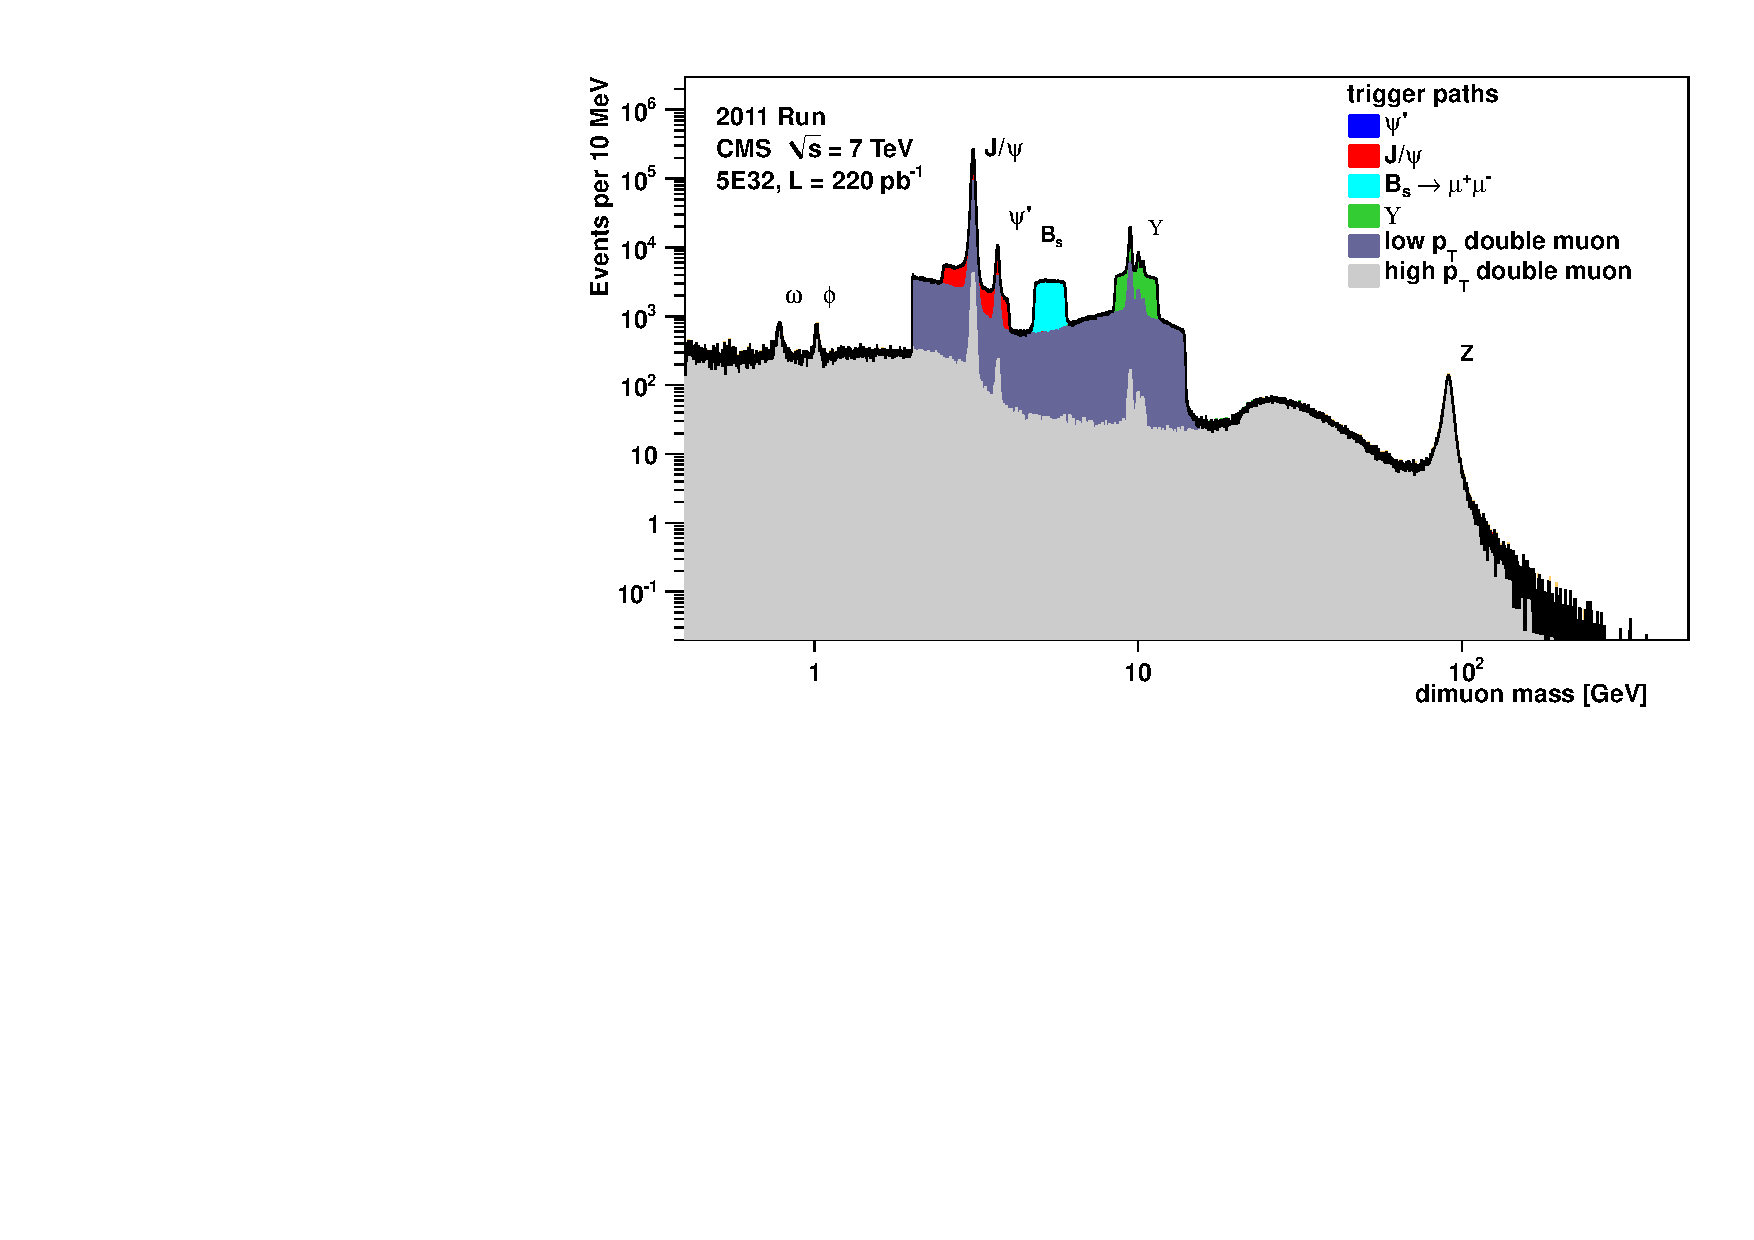
\includegraphics[width=0.8\textwidth]{Figures/dimuMass_2011Run_5E32.pdf}
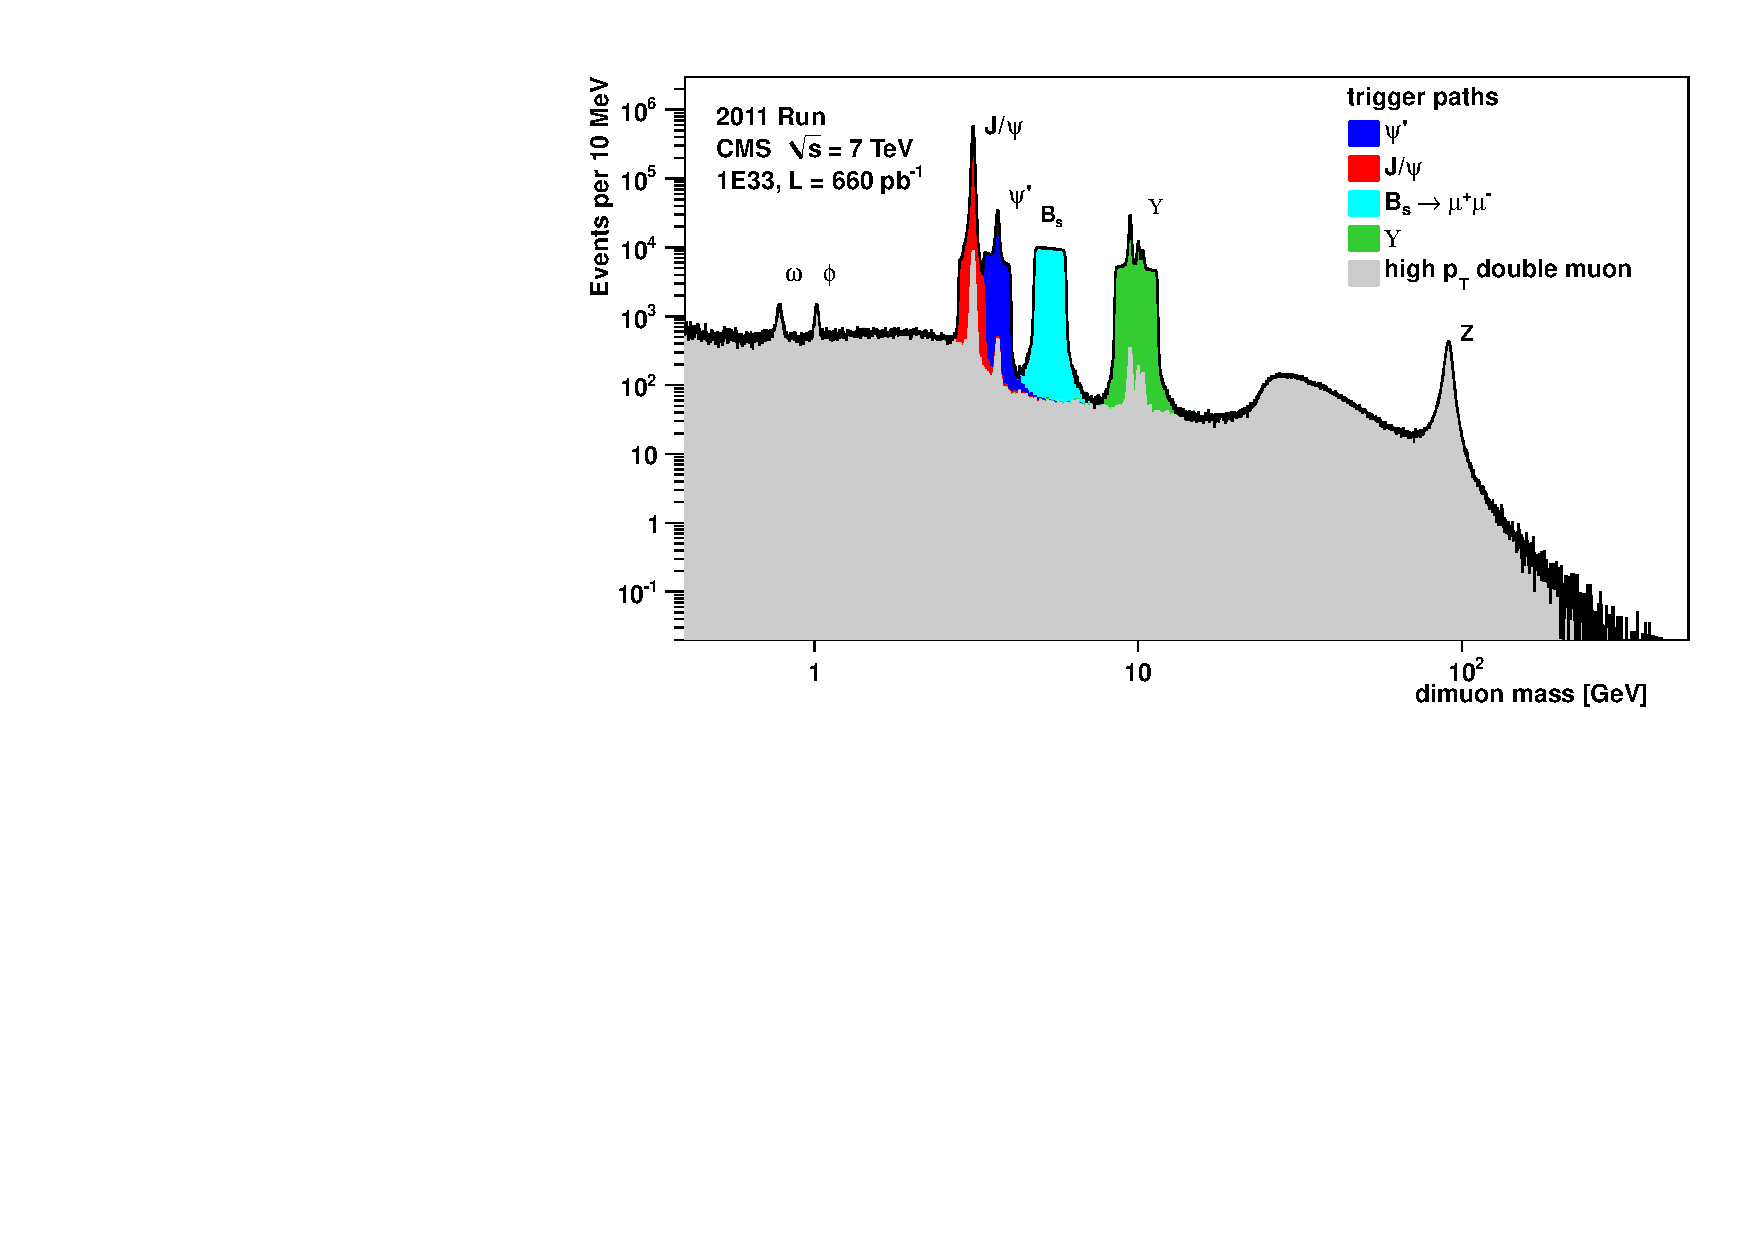
\includegraphics[width=0.8\textwidth]{Figures/dimuMass_2011Run_1E33.pdf}
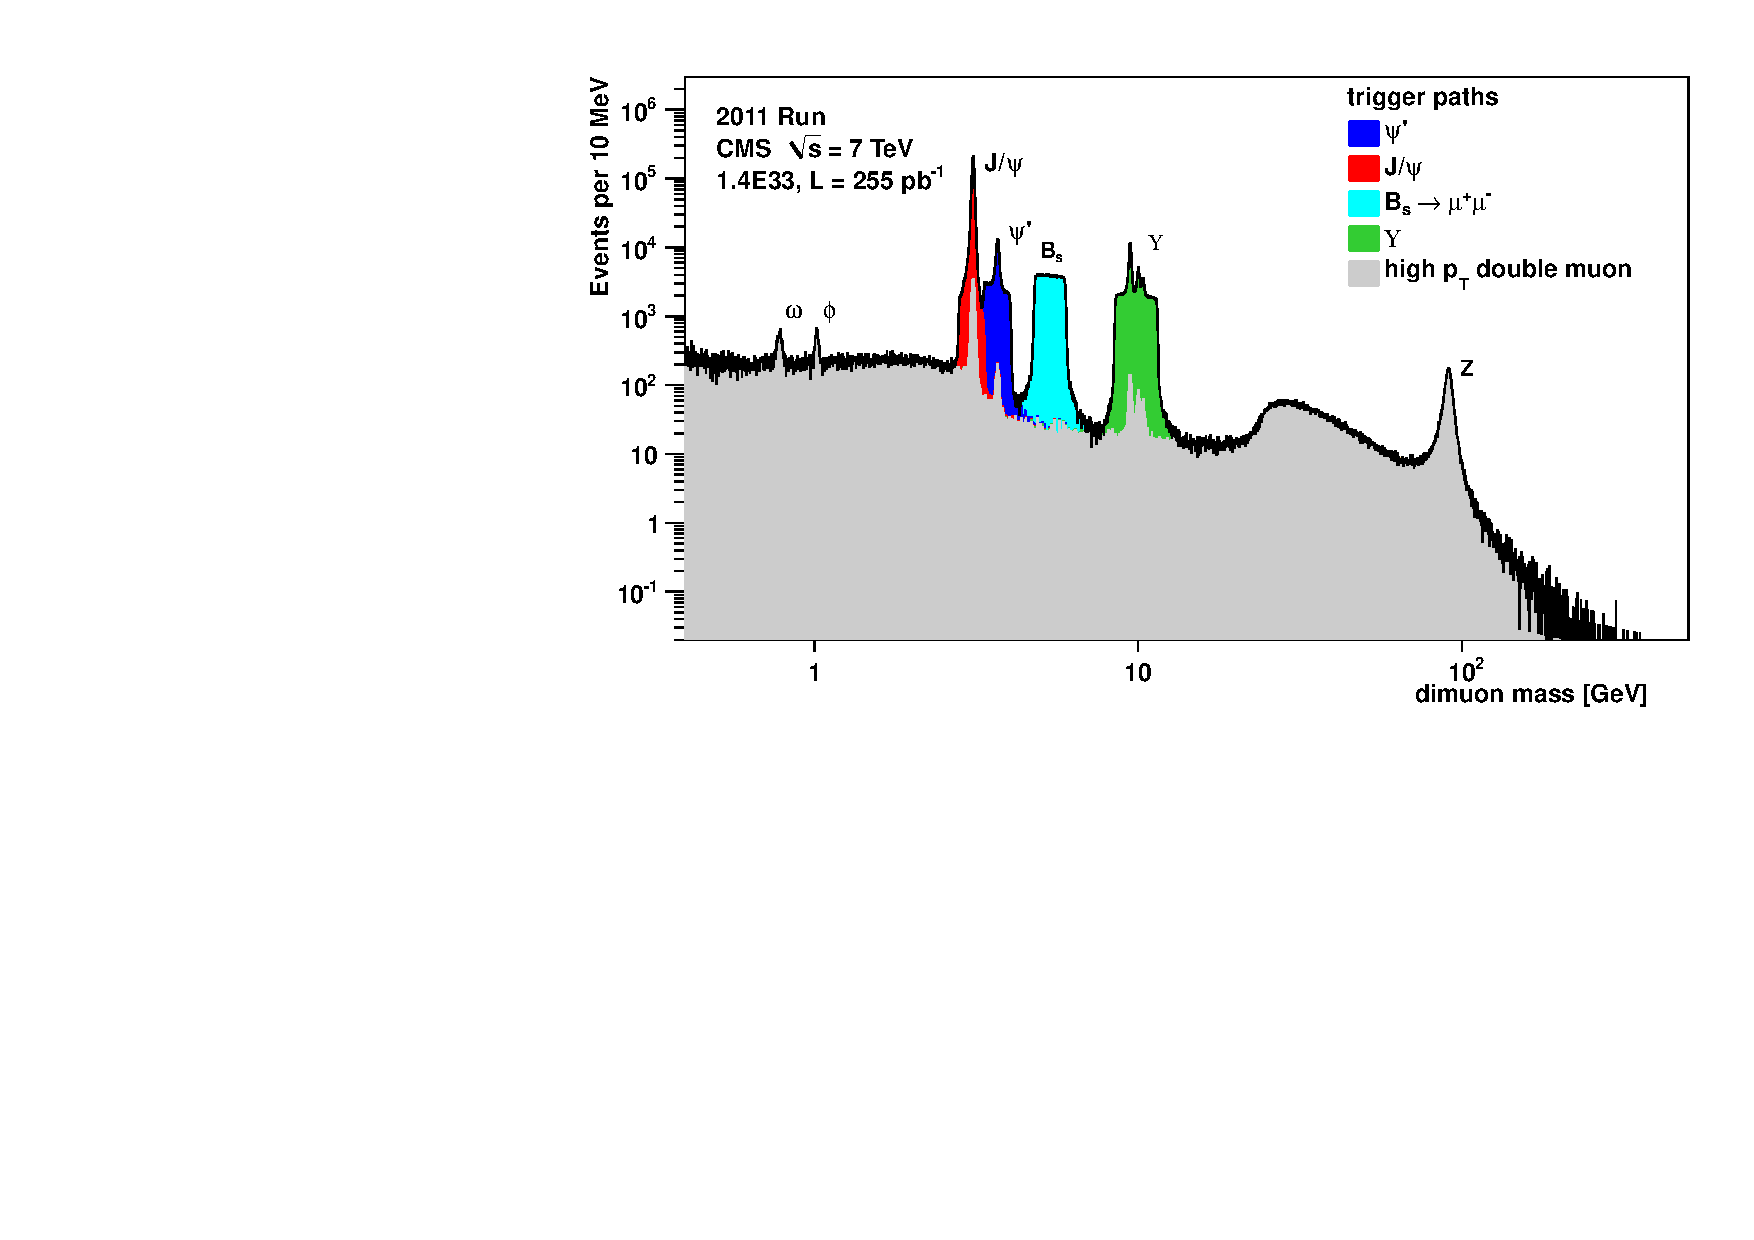
\includegraphics[width=0.8\textwidth]{Figures/dimuMass_2011Run_1p4E33.pdf}
%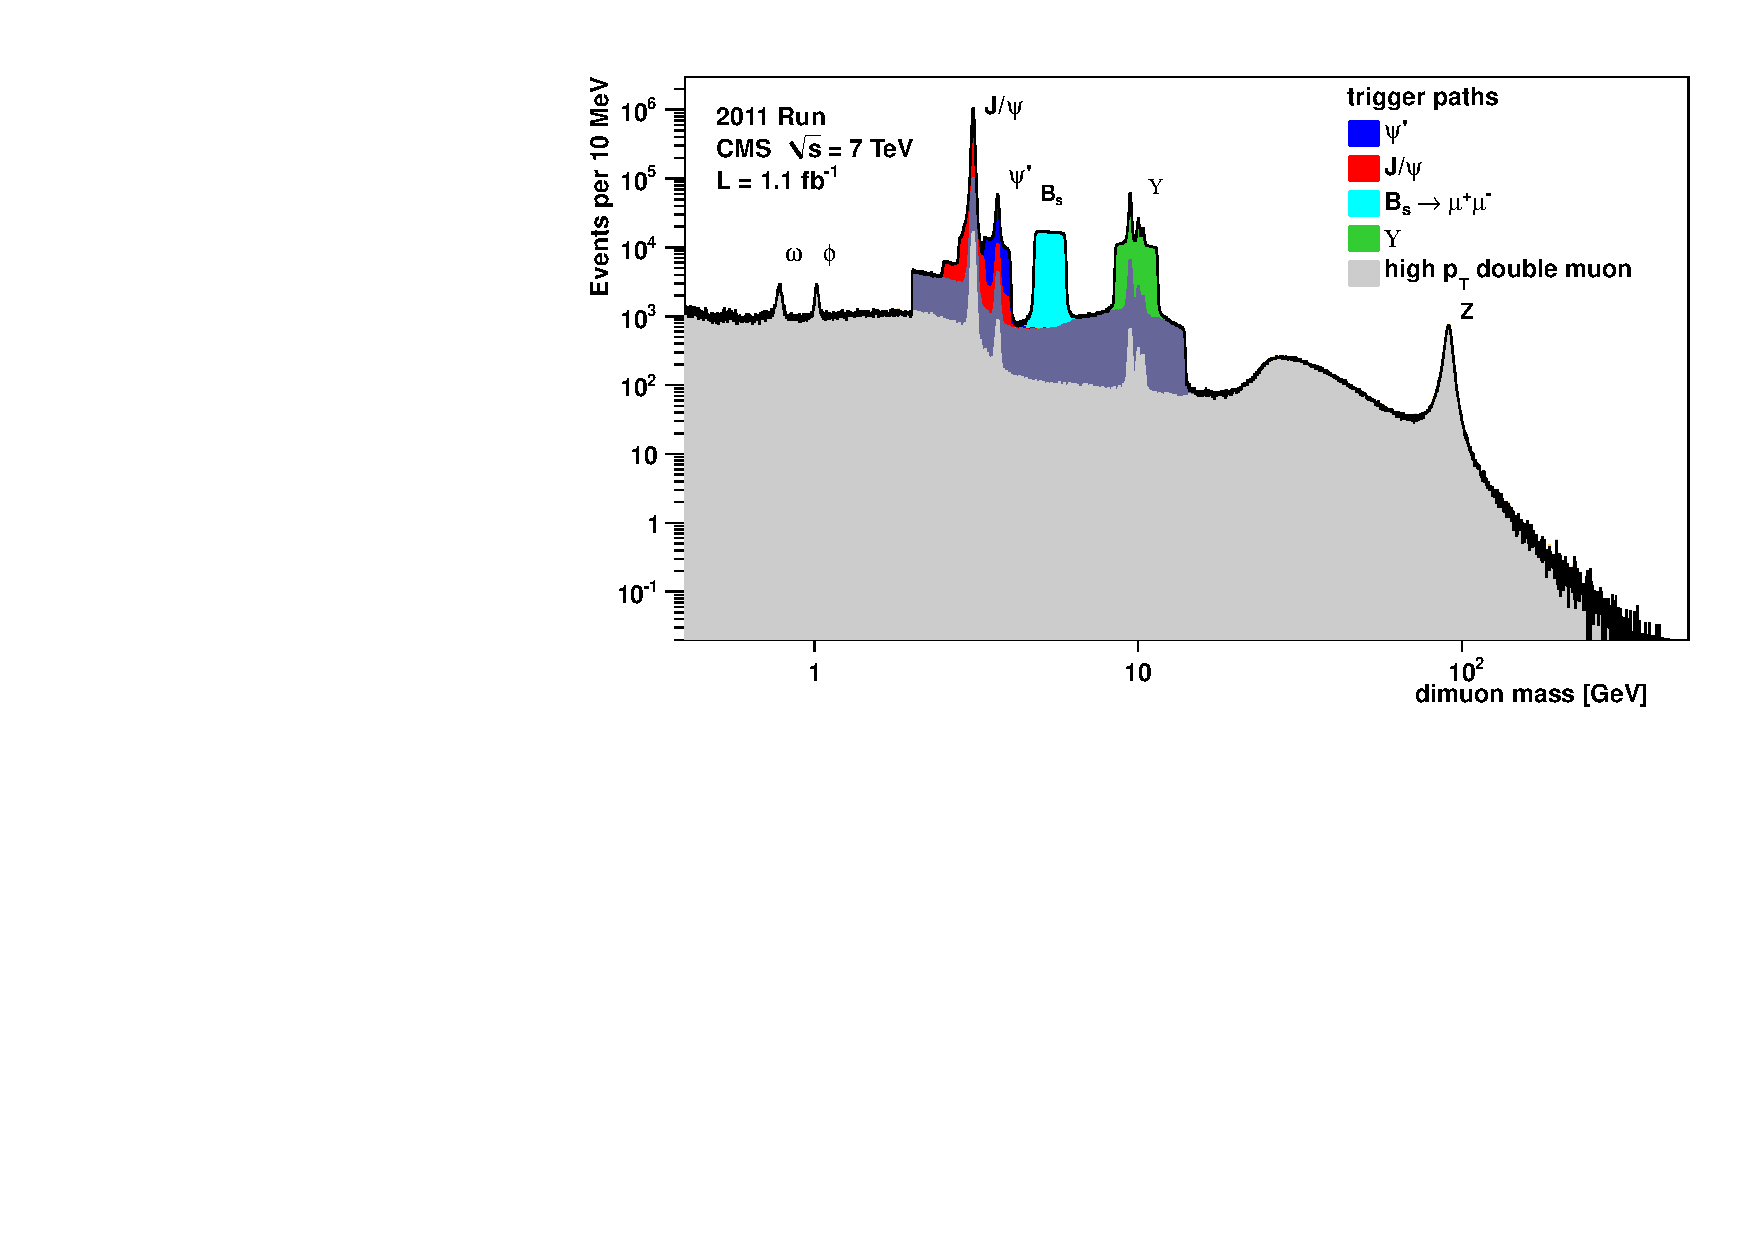
\includegraphics[width=0.8\textwidth]{Figures/dimuMass_2011Run_1fb.pdf}
\caption{Dimuon mass distributions, using the offline reconstructed
  variables, triggered by the trigger paths listed in the legend
  box. The figures reflect the trigger menu during the 5E32 (top),
  1E33 (middle) and 1.4E33 (bottom) data taking periods, up to the end
  of June 2011.}
% , as well as a time integrated representation, containing the
% previous 5E32 trigger menu, representing the first 1,1 fb$^{-1}$, as
% collected up to end of June 2011.}
\label{fig:MuOnia-trig}
\end{figure}

The two types of efficiency triggers exist in the following instances:
Mu5\_L2Mu2\_Jpsi, Mu5\_Track2\_Jpsi and Mu7\_Track7\_Jpsi. The latter
two are both aimed to study the same kind of efficiency, but with a
different \pt\ coverage of the probe muon, $p_{\rm T} \gtrsim 2$ and
7~GeV/$c$, respectively. The high \pt\ instance covers the region
where the efficiencies should reach their saturation values. Because
of the higher trigger rate, the low \pt\ version has a significantly
larger prescale than its ``high \pt'' counterpart.

The studies presented here were obtained by covering the run periods
 summarized in Table~\ref{tab:PDs}.
\begin{table}[htb]
  \centering \caption{Datasets used for the \tnp\ studies discussed in this note.}
\begin{tabular}{|c|c|c|}\hline
data set & trigger menu & run range \\ \hline
Run2011A-May10ReReco-v1 & 5E32 & $160432 - 163870$ \\
Run2011A-PromptReco-v4 & 1E33$+$1.4E33 & $165088 - 167675$ \\
Run2011A-PromptReco-v5 & 2E33 & $170723 - 172619$ \\
Run2011A-PromptReco-v6 & 2E33$+$3E33 & $172621 - 173693$ \\ \hline
Run2011B-PromptReco-v1 & 3E33$+$5E33 & $175832 - 180252$ \\ \hline
\end{tabular}
\label{tab:PDs}
\end{table}
The events collected during the 5E32 run period (May10ReReco) are
exclusively used for the study of the muon reconstruction efficiencies
and the efficiencies of the quality cuts, because the trigger
settings changed several times throughout this period. Starting from
the 1E33 trigger menu, only minor L1 changes were
performed~\cite{luigiTWiki}, which should have negligible impact on
the trigger efficiency. The only L1 trigger change worth mentioning is
the one effective from run 175971, when the global muon trigger (GMT)
changed the assignment of the confirmed candidates' \pt\ value.  In
case the RPC as well as the DT or CSC detector systems measured the
candidate muon at the same time, instead of returning the smaller \pt\
value to the global trigger, it was changed to return a \pt\ value
given through a preprogramed rank instead (\texttt{byMinPt} became
\texttt{byRank}). Furthermore, during the run period $165088 - 172868$
all dimuon triggers in the \texttt{MuOnia} PD used the "L1\_DoubleMu0"
seed, while afterwards the "L1\_DoubleMu0\_HighQ" was used. That
defines the following three distinct run periods concerning L1 trigger
efficiency studies:
\begin{itemize}
\item $165088 - 172868$: L1\_DoubleMu0 seed
\item $173236 - 175970$: L1\_DoubleMu0\_HighQ seed
\item $> 175971$: GMT changed \pt\ assignment
\end{itemize}

The L2 settings were not changed throughout the 1E33$-$5E33 data
taking period. The L3 reconstruction settings were only changed during
the 5E33 trigger menu (starting from run 178380), when the transverse
momentum was taken from the measurement in the tracker only, while it
used to be from the global fit.

The \tnp\ skims were produced using the following two data
certification files for the May10ReReco and PromptReco data,
respectively:
\begin{itemize}
\item
  Cert\_160404-163869\_7TeV\_May10ReReco\_Collisions11\_JSON\_MuonPhys\_v3.txt
\item
  Cert\_160404-180252\_7TeV\_PromptReco\_Collisions11\_JSON\_MuonPhys.txt  
\end{itemize}

%%%%%%%%%%%%%%%%%%%%%%%%%%%%%%%%%%%%%
\section{Selection of tag and probe muons}\label{sec:selection}

It is important that the matching criteria between the reconstructed
(RECO) and trigger (HLT) muons be identical for the physics data
analysis and for the corresponding \tnp\ studies. In the present study
this is ensured given that our PAT Tuplizer (Onia2MuMuPAT.cc)
simultaneously produces the muon pairs for the data analysis as well
as for the study of the \tnp\ efficiencies, commonly using the PAT
muon matching settings as defined in \\
\texttt{MuonAnalysis/MuonAssociators/python/patMuonsWithTrigger\_cff.py}. In
particular, the matching cones in $\Delta R$ between the RECO and
trigger muons are 0.3 (L1), 0.3 (L2) and 0.1 (L3), respectively for
the trigger muons at different levels of HLT. The larger cone size for
L1 and L2 muons allows for the larger measurement uncertainties, given their
limited resolution. The corresponding matching cone size for the CtfTrack
in the MuX\_TrackY\_Jpsi trigger paths is 0.1, in tune with the one of
L3 muons. No matching requirement is performed concerning the RECO and
HLT muon's transverse momenta.

In order to use the single muon efficiencies for physics data
analyses, we apply fiducial cuts to the tags, as well as probes, in
order to define an event sample faithfully representing the
distribution of the corresponding physics data analysis sample. These
single muon kinematical cuts have been obtained on the basis of MC
simulations, requesting that the single muon reconstruction efficiency
be higher than 50\%, see Fig. ~\ref{fig:glbMu-envelope}. In the
present document we consider two sets of fiducial cuts: Set a)
dedicated to all studies using (inclusive) tracker muons; and Set b)
setting a tighter cut on the muon's \pt. In the following, we will
refer to the two sets as ``tracker50'' and ``global50'' cuts, respectively.
\begin{figure}[htb]
\centering
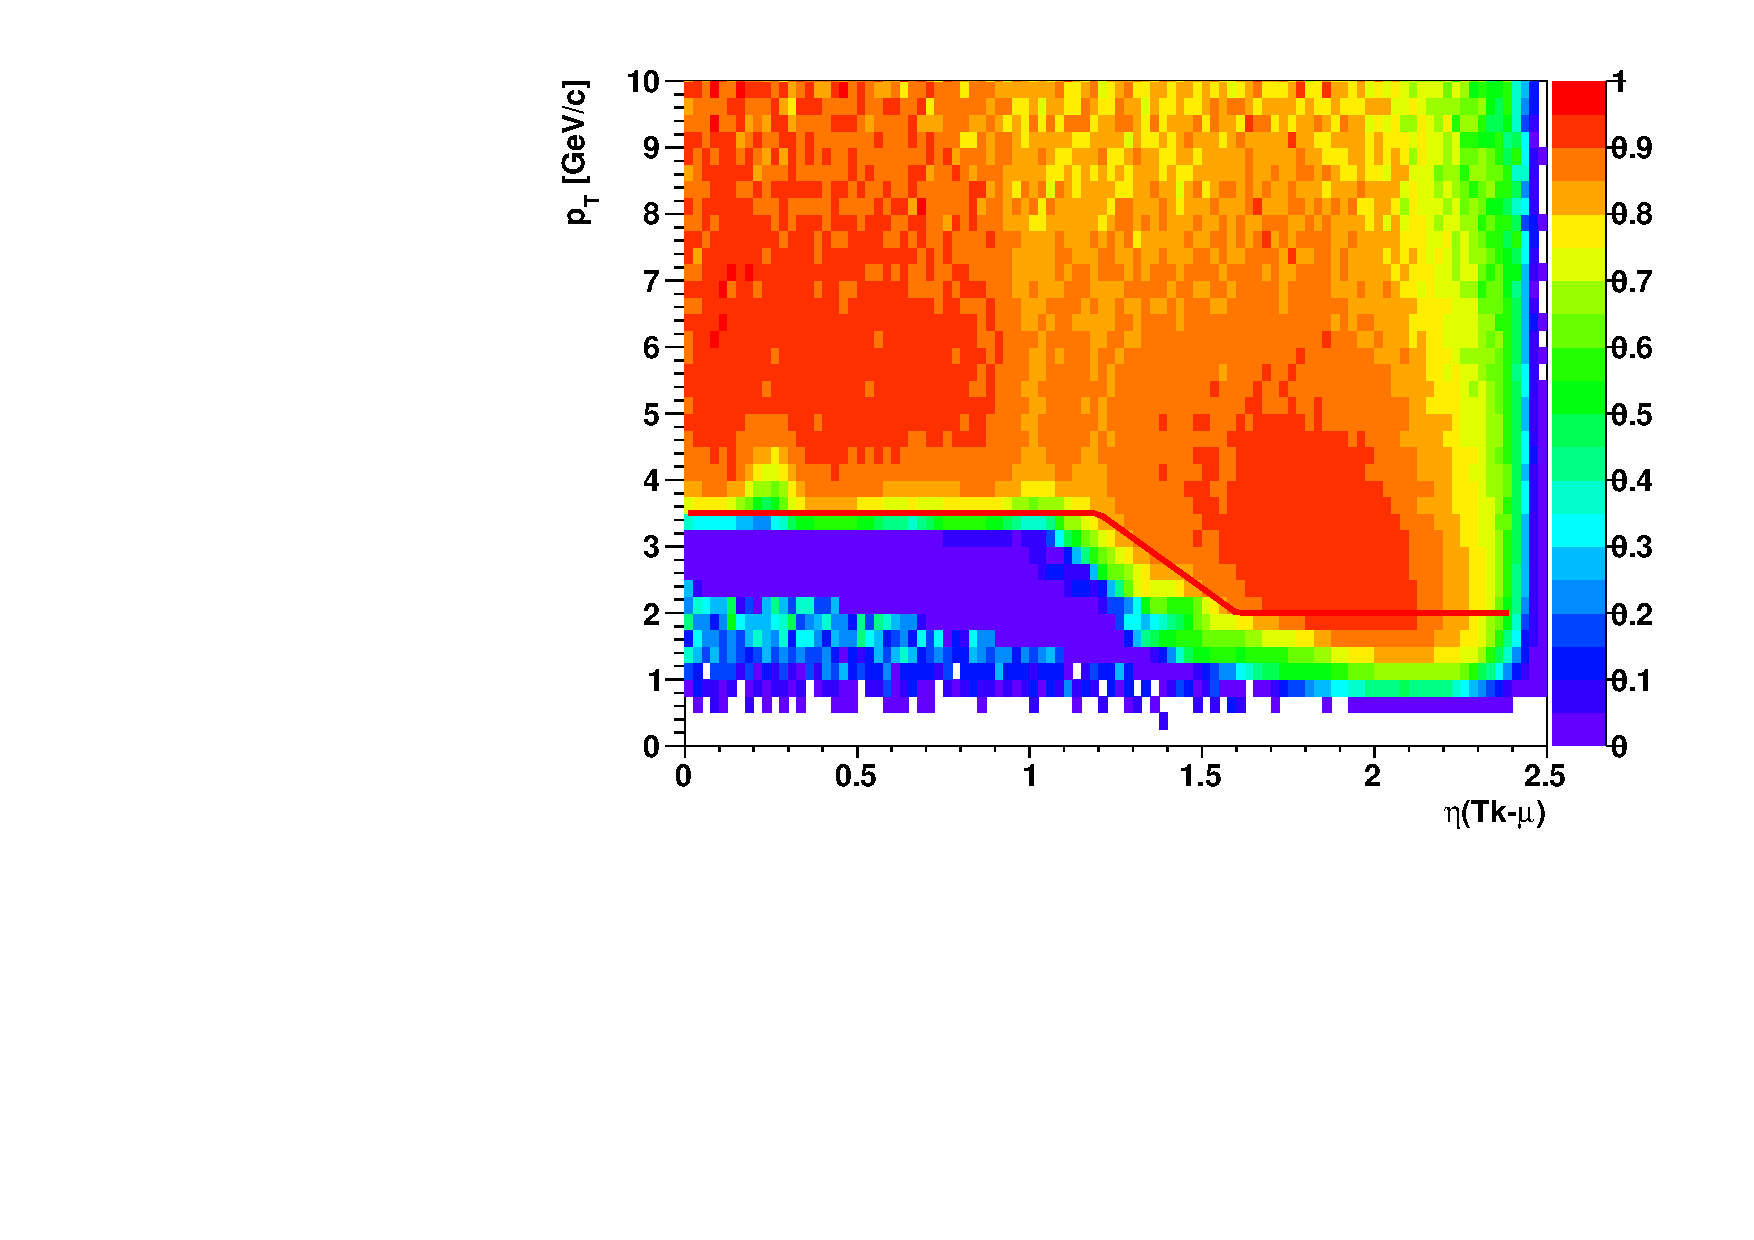
\includegraphics[width=0.49\textwidth]{Figures/recoEff_pT_vs_eta_Tkmu.pdf}
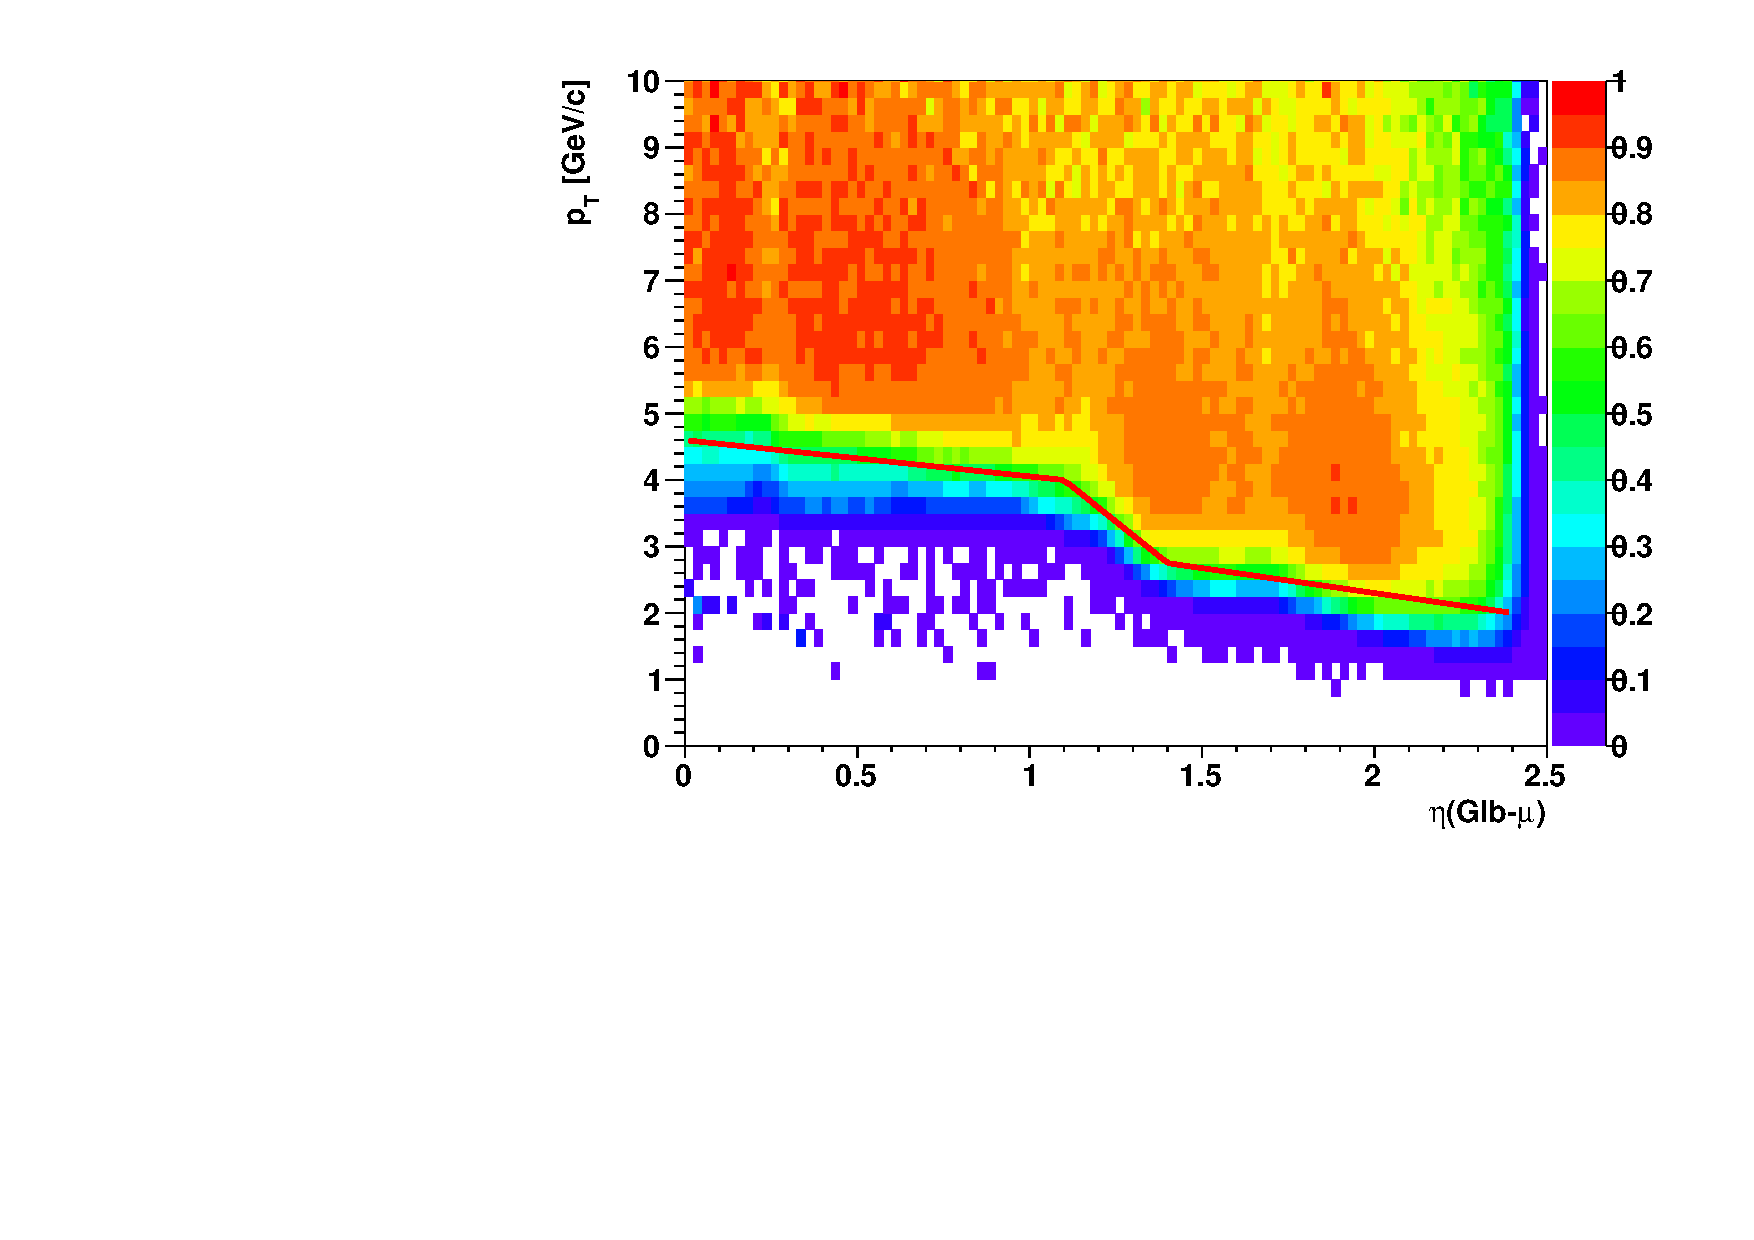
\includegraphics[width=0.49\textwidth]{Figures/recoEff_pT_vs_eta_Glbmu.pdf}
\caption{MC based reconstruction efficiencies as a function of \pt\
  and $|\eta|$, for tracker muons without (left) and with (right)
  requesting that they are also reconstructed as global muons. The red
  line indicates the kinematic fiducial cut applied to the tag and
  probe muons, in the loose case (left) and tight case (right).}
\label{fig:glbMu-envelope}
\end{figure}

For global muons the red line indicates the 50\% border line, which can
be described by linear cuts (the ``global50'' cuts) in the following way:
\begin{eqnarray}\nonumber
|\eta| < 1.1:& & \,\, p_{\rm T, min} = 4.6 \to 4.0~{\rm GeV/}c \\ \nonumber
1.1 < |\eta| < 1.4:& &\,\, p_{\rm T, min} = 4.0 \to 2.75~{\rm GeV/}c \\ \nonumber
1.4 < |\eta| < 2.4:& &\,\, p_{\rm T, min} = 2.75 \to 2~{\rm GeV/}c
\end{eqnarray}
The corresponding efficiencies were studied in 2D using the following
bins, which reflect the above \pt\ and $|\eta|$ borders:
\begin{itemize}
\item $p_{\rm T}$ = {2, 2.75, 4, 4.6, 6, 8, 10, 15, 50}~GeV/$c$
\item $|\eta|$ = {0, 0.2, 0.3, 0.8, 1.2, 1.4, 2.1}
\end{itemize}

The corresponding cuts for tracker muons (the ``tracker50'' cuts) are also
based on the 50\% reconstruction efficiency line, but need to be
modified for $|\eta| > 1.6$ due to the fact that the \tnp\ studies are
limited to the range $p_{\rm T} > 2$~GeV/$c$. The corresponding cuts
can be summarized as:
\begin{eqnarray}\nonumber
|\eta| < 1.2:& & \,\, p_{\rm T, min} = 3.5~{\rm GeV/}c \\ \nonumber
1.2 < |\eta| < 1.6:& &\,\, p_{\rm T, min} = 3.5 \to 2.0~{\rm GeV/}c \\ \nonumber
1.6 < |\eta| < 2.4:& &\,\, p_{\rm T, min} = 2~{\rm GeV/}c
\end{eqnarray}
Similarly, the corresponding 2D efficiency calculations use bins that
reflect the given \pt\ and $|\eta|$ borders:
\begin{itemize}
%\item $p_{\rm T}$ = {2.0, 2.75, 3.5, 4.5, 5.5, 7.0, 10, 15,
%50}~GeV/$c$
\item $p_{\rm T}$ = {2.0, 2.5, 3.0, 3.5, 4.0, 4.5, 5.0, 5.5, 6, 7, 8, 10, 15, 20, 100}~GeV/$c$
\item $|\eta|$ = {0, 0.2, 0.3, 0.6, 0.8, 1.2, 1.6, 2.1, 2.4}
\end{itemize}

Throughout the whole document we will show figures prepared with the
``tracker50'' cuts; the corresponding efficiencies for ``global50'' cuts are
summarized in Table~\ref{tab:eff-glb}. The graphical representation can be
found in Ref.~\cite{tnp-bph}.

%%%%%%%%%%%%%%%%%%%%%%%%%%%%%%%%%%%%%
\section{Setup of the \tnp\ fitter scripts}\label{sec:setup}

The \tnp\ producer script is defined not only to prepare all the
needed variables for the corresponding fitter scripts, but also to
filter on events triggered by either the HLT\_MuX\_TrackY\_Jpsi or
the HLT\_MuX\_L2MuY\_Jpsi efficiency trigger paths.

The way the fitter scripts are set up is done in a similar fashion for
all the 4 single muon efficiencies: the tag muon is matched to the L3
leg (``HLT\_MuX") of the efficiency trigger paths. The probe is then
matched to the second leg in the efficiency path, i.e. the ``TrackY"
in the case of the muon related efficiency studies, or the ``L2MuY" object
in the case of the tracker related efficiencies. The passing probes
are the fraction of all probes that pass a given, well defined
criterion, to be discussed in the individual sections below.

In the case of the efficiency of the trigger dimuon vertexing module,
which is used in all the quarkonium physics triggers of the
\texttt{MuOnia} PD, a slightly different procedure needs to be
adopted, given that it is not a single muon but rather a dimuon whose
efficiency is probed: the \tnp\ skim needs to be prepared with the
option
\begin{verbatim}
arbitration   = cms.string("OnePair")
\end{verbatim}
In this way the pair becomes the probe. The efficiency of any of the
vertexing modules (last L3 filter in any of the quarkonia trigger
paths) can be studied with respect to the specially designed trigger
path HLT\_Dimuon0\_Jpsi\_NoVertexing, which is available from the 2E33
trigger menu onwards (run 170249) and does not contain the vertexing
module in its trigger path. In the current study, we use the vertexing
module of the HLT\_Dimuon0\_Jpsi trigger path, given that its
configuration is identical to the ones of the inclusive \jpsi, \psip\
and $\Upsilon$ trigger paths: it simply requests that the dimuon
secondary vertex has a fit $\chi^2$ probability larger than
0.5\,\%. Given that the HLT\_Dimuon0\_Jpsi trigger path had a prescale
factor different from the one of the HLT\_Dimuon0\_Jpsi\_NoVertexing,
its prescale factor needs to be accounted for in the efficiency
measurement.

%%%%%%%%%%%%%%%%%%%%%%%%%%%%%%%%%%%%%
\section{Number of events}

Efficiency triggers usually have prescale factors adapted to the
increase in instanteous luminosity such that their rate stays overall
constant. In the following we discuss the number of events collected
in the efficiency triggers throughout the individual trigger menus in
2011, as well as how they are distributed across the single muon \pt\
and $\eta$ plane. We discuss the number of events surviving the
fiducial cuts, using the ``tracker50'' set of cuts, that enter the
efficiency calculation. The quoted numbers refer to the number of
fitted \jpsi's considered in the given efficiency evaluation.
\begin{figure}[htb]
\centering
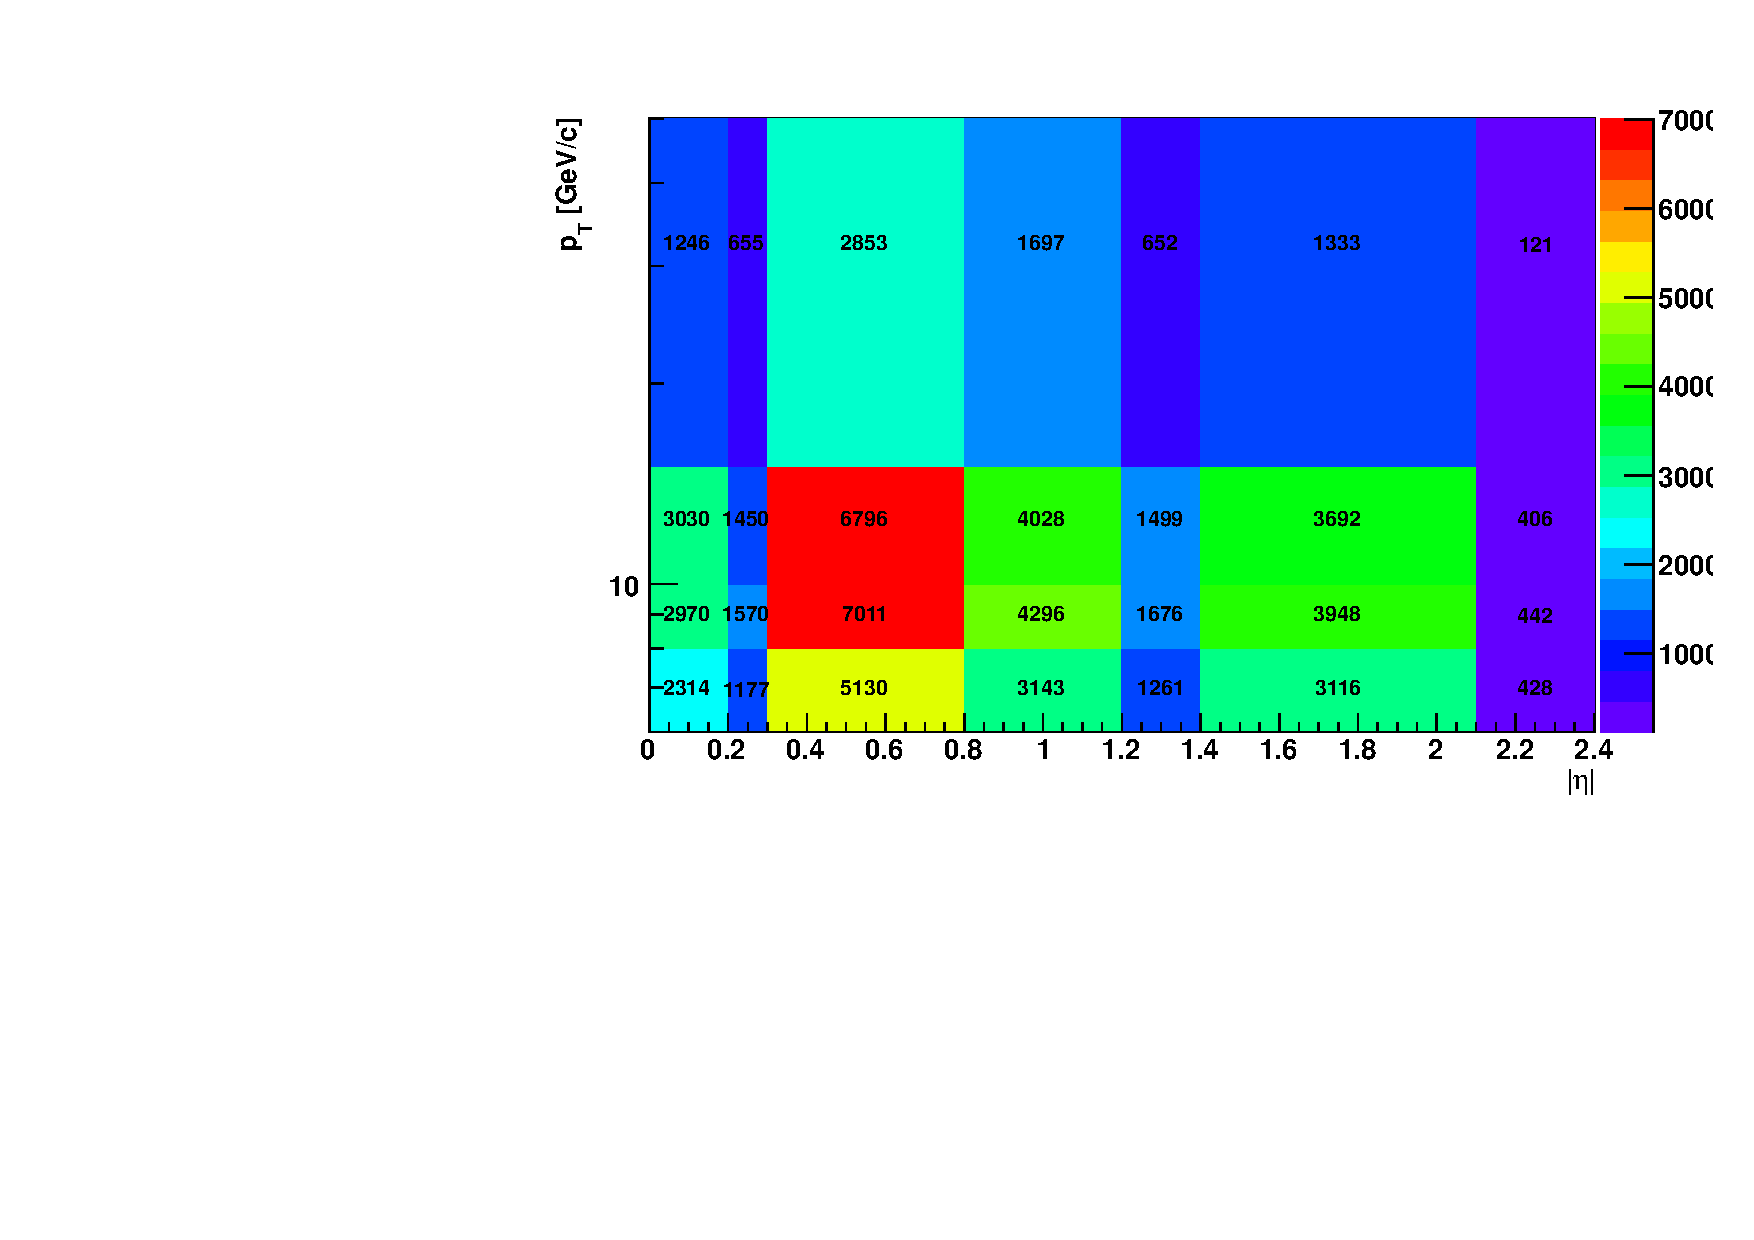
\includegraphics[width=0.52\textwidth]{Figures/nbEvents_L1L2-Mu7Track7-run1-globalCuts50-17Oct2011.pdf}
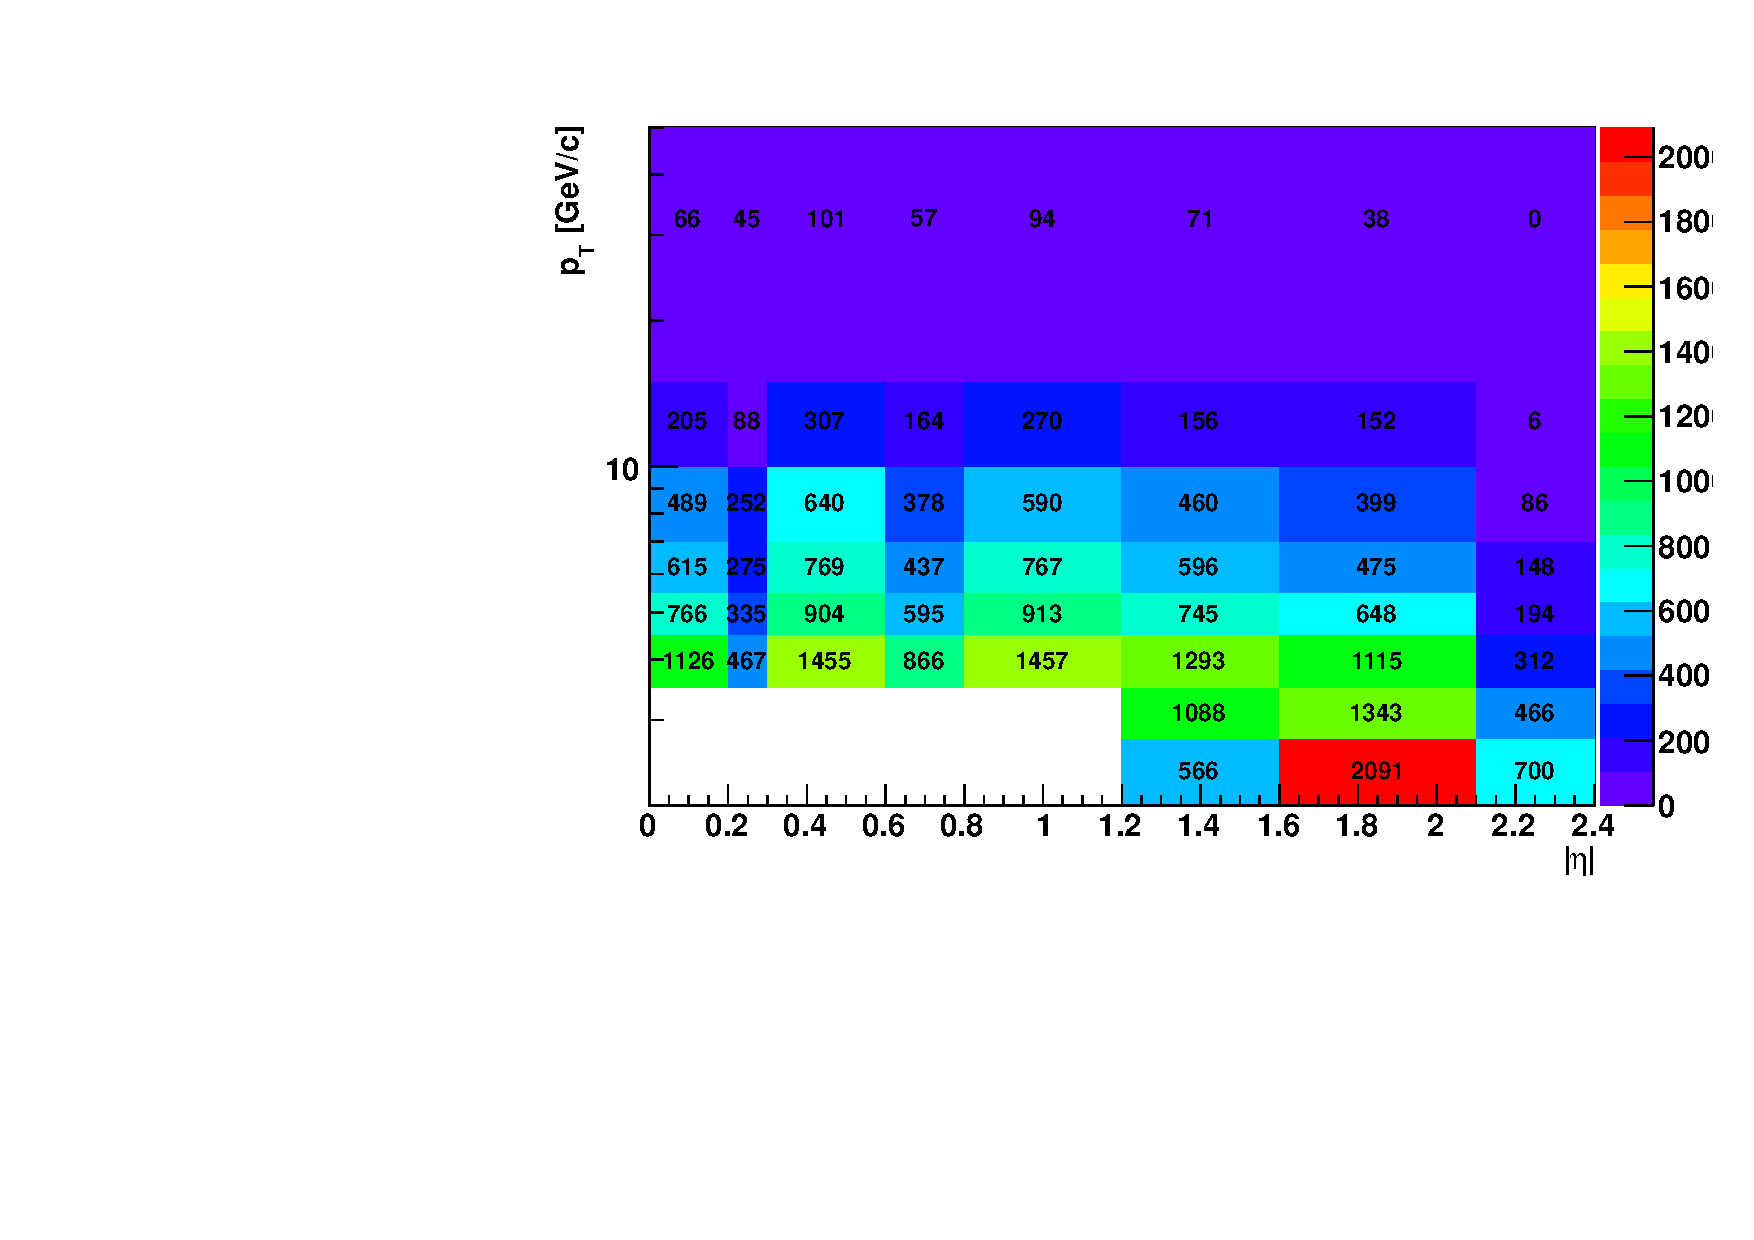
\includegraphics[width=0.47\textwidth]{Figures/nbEvents_L1L2-Mu5Track2-run1-TrkCuts50-20Oct2011.pdf}
\caption{Number of events as a function of the probe muon's \pt\ and
  $|\eta|$, collected with the HLT\_Mu7\_Track7\_Jpsi (left) and
  HLT\_Mu5\_Track2\_Jpsi (right) trigger paths during the period
  $165088 - 172868$, after the ``BMuQual'' cuts, as used in the
  studies of the L1$\cdot$L2 trigger efficiencies.}
\label{fig:singleMuStat}
\end{figure}

Figure~\ref{fig:singleMuStat} shows how the collected statistics is
distributed across the single muon's \pt\ and $|\eta|$ after applying
the ``BMuQual'' cuts, as is used for the studies of the L1$\cdot$L2
trigger efficiencies. All the events collected with the
"L1\_DoubleMu0" trigger seed ($165088 - 172868$) have been integrated.

%Integrating over \pt\ and $|\eta|$, the collected yield used for the
%efficiency studies is distributed over the run period as summarized in
%Table~\ref{tab:timeEv-statistics}.
%\begin{table}[htb]
%  \centering \caption{Statistics used in the fits for the individual
%    trigger efficiencies, separating the 5 different run
%    periods. Numbers are in units of 1000.}
%\begin{tabular}{|c||c|c|c|c|}\hline
%HLT menu & $\epsilon_{\rm muonID}$ & $\epsilon_{\rm muQual}$ & $\epsilon_{\rm
%  L1\cdot L2}$ & $\epsilon_{\rm L3}$ \\ \hline
%1E33 & 234 & 423 & 41 & \\ \hline
%1.4E33 & 28 & 23 & 4.9 & \\ \hline
%2E33 & 103 & 84 & 18 & \\ \hline
%3E33 & 135 & 102 & 18 & \\ \hline
%5E33 & 83 & 75 & 14 & \\ \hline
%\end{tabular}
%\label{tab:timeEv-statistics}
%\end{table}

Integrating over \pt\ and $|\eta|$, the collected yield used for the
efficiency studies is distributed over the individual run periods in
the following way:
\begin{description}
\item[MuonID:] $160404 - 173692$ (RunA): 80k; $175832 - 180252$ (RunB): 30k
\item[MuonQual:] $160404 - 173692$ (RunA): 500k; $175832 - 180252$
  (RunB): 120k
\item[L1$\cdot$L2:] $165088 - 172868$: 26k; $173236 - 175970$: 2.2k;
  $175971 - 180252$ (RunB): 13k
\item[L3:] $165088 - 173692$: 240k; $178380 - 180252$: 28k
\end{description}

The events triggered with the HLT\_MuX\_TrackY\_Jpsi trigger paths are
very impure, usually not containing a real \jpsi\ in the event. The
requirement on the second ``leg'' to be a track reconstructed in the
Silicon tracker only is not a guarantee to become the second muon of a
possible \jpsi. However, only in this way one assures that the
measurement of the reconstruction efficiencies are not biased. The
fraction of events containing a true \jpsi\ in the
HLT\_Mu5\_Track2\_Jpsi and HLT\_Mu7\_Track7\_Jpsi trigger paths is
only 20 (30)\,\% (the above quoted numbers refer to the available
number of \jpsi's, not counting the background). As will be shown in
Section~\ref{sec:muonID}, the ``Failing Probes'', hence, are affected
by a large continuum background.

On the other hand, the events collected with the HLT\_MuX\_L2Mu2\_Jpsi
are rather pure and most events contain a real \jpsi, i.e. the
corresponding background is very small.

%%%%%%%%%%%%%%%%%%%%%%%%%%%%%%%%%%%%%
\section{MC sample}

The \tnp\ studies are performed in an analogous way on a \jpsi\ MC
sample. For this purpose, a private MC simulation was set up that
contains realistic L1 and HLT trigger menu settings, as were used
during the 1E33, 1.4E33, 2E33 and 3E33 ``RunA" data taking period in
2011. The simulation, using a flat \jpsi\ gun with flat \pt\ (in the
range $3 < p_{\rm T} < 50$~GeV/$c$) and rapidity ($|y| < 1.3$)
distributions, was set up in CMSSW\_4\_2\_9\_HLT1\_hltpatch1 and
global tag START42\_V14A::All. The following packages were
additionally checked out:
\begin{itemize}
\item V00-00-00-00   Configuration/AlCa                              
\item V04-01-12      Configuration/EventContent                      
\item V01-02-00      Configuration/HLT                               
\item V02-24-02      FastSimulation/Configuration                    
\item V00-04-01      FastSimulation/Muons                            
\item V12-02-00      HLTrigger/Configuration                         
\item V00-10-01      HLTrigger/Egamma                                
\item V03-08-07      HLTrigger/HLTanalyzers                          
\item V00-04-01      HLTrigger/JetMET                                
\item V02-11-11      HLTrigger/Muon 
\end{itemize}
In order to use the L1 trigger settings of the above data taking
period, summarized in Ref.~\cite{luigiTWiki}, an additional piece of
code was added to the simulation config file, summarized in Appendix
A. An HLT menu was prepared that contained all the \jpsi\ trigger
paths that were run during the four different running periods,
including the different L1 trigger seeds mentioned in
Section~\ref{sec:dataSets}.

The simulation was limited to the \jpsi\ rapidity range $|y| <
1.3$. Since the single muons are highly correlated with the dimuon's
kinematics, this simulation does not contain muons beyond $|\eta| >
1.4$, especially for high \pt.

%%%%%%%%%%%%%%%%%%%%%%%%%%%%%%%%%%%%%
\section{Offline muon reconstruction efficiency}\label{sec:muonID}

The probes for the muon reconstruction efficiencies are offline tracks
of the collection \texttt{generalTracks} with two additional requests:
\pt\ above a certain threshold, lower than what can be reasonably
reconstructed as a muon; matched to the \texttt{TrackY} leg of the
efficiency trigger path. As passing probes we consider
\begin{itemize}
\item arbitrated tracker muons or
\item global muons which are also arbitrated tracker muons, have a
  reduced global fit-$\chi^2$ smaller than 20 and have
  \texttt{numberOfValidMuonHits} $>0$,
\end{itemize}
shortly referred to as ``BMuons".

\begin{figure}[htb]
\centering
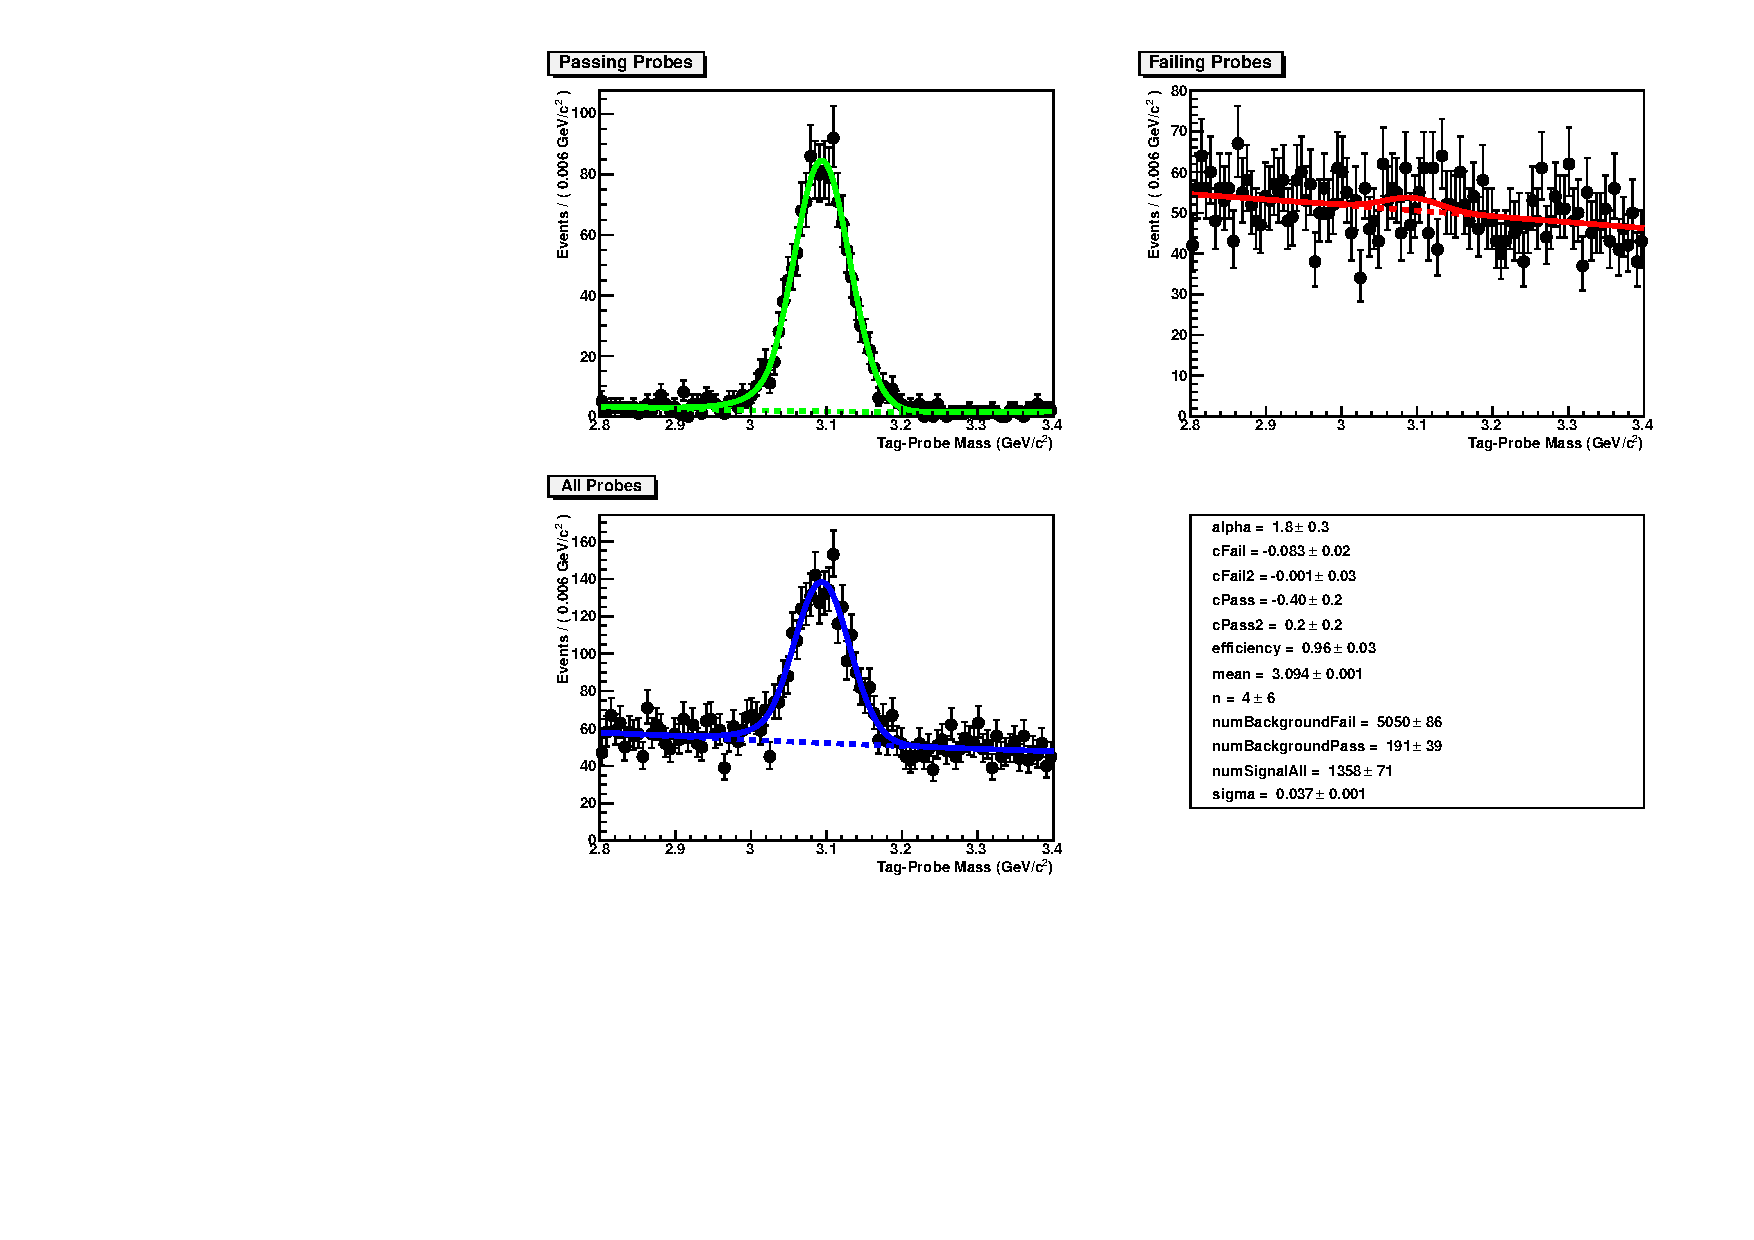
\includegraphics[width=\textwidth]{Figures/MuonID_abseta4_pt1.pdf}
\caption{Example of the fitted mass distributions of ``Passing",
  ``Failing" and ``All Probes" in case of the muon reconstruction
  efficiencies for one particular bin ($1.2 < |\eta| < 1.4$ and $2.75
  < p_{\rm T} < 4$~GeV/$c$).}
\label{fig:muonID-abseta4_pt1}
\end{figure}

\begin{figure}[p]
\centering
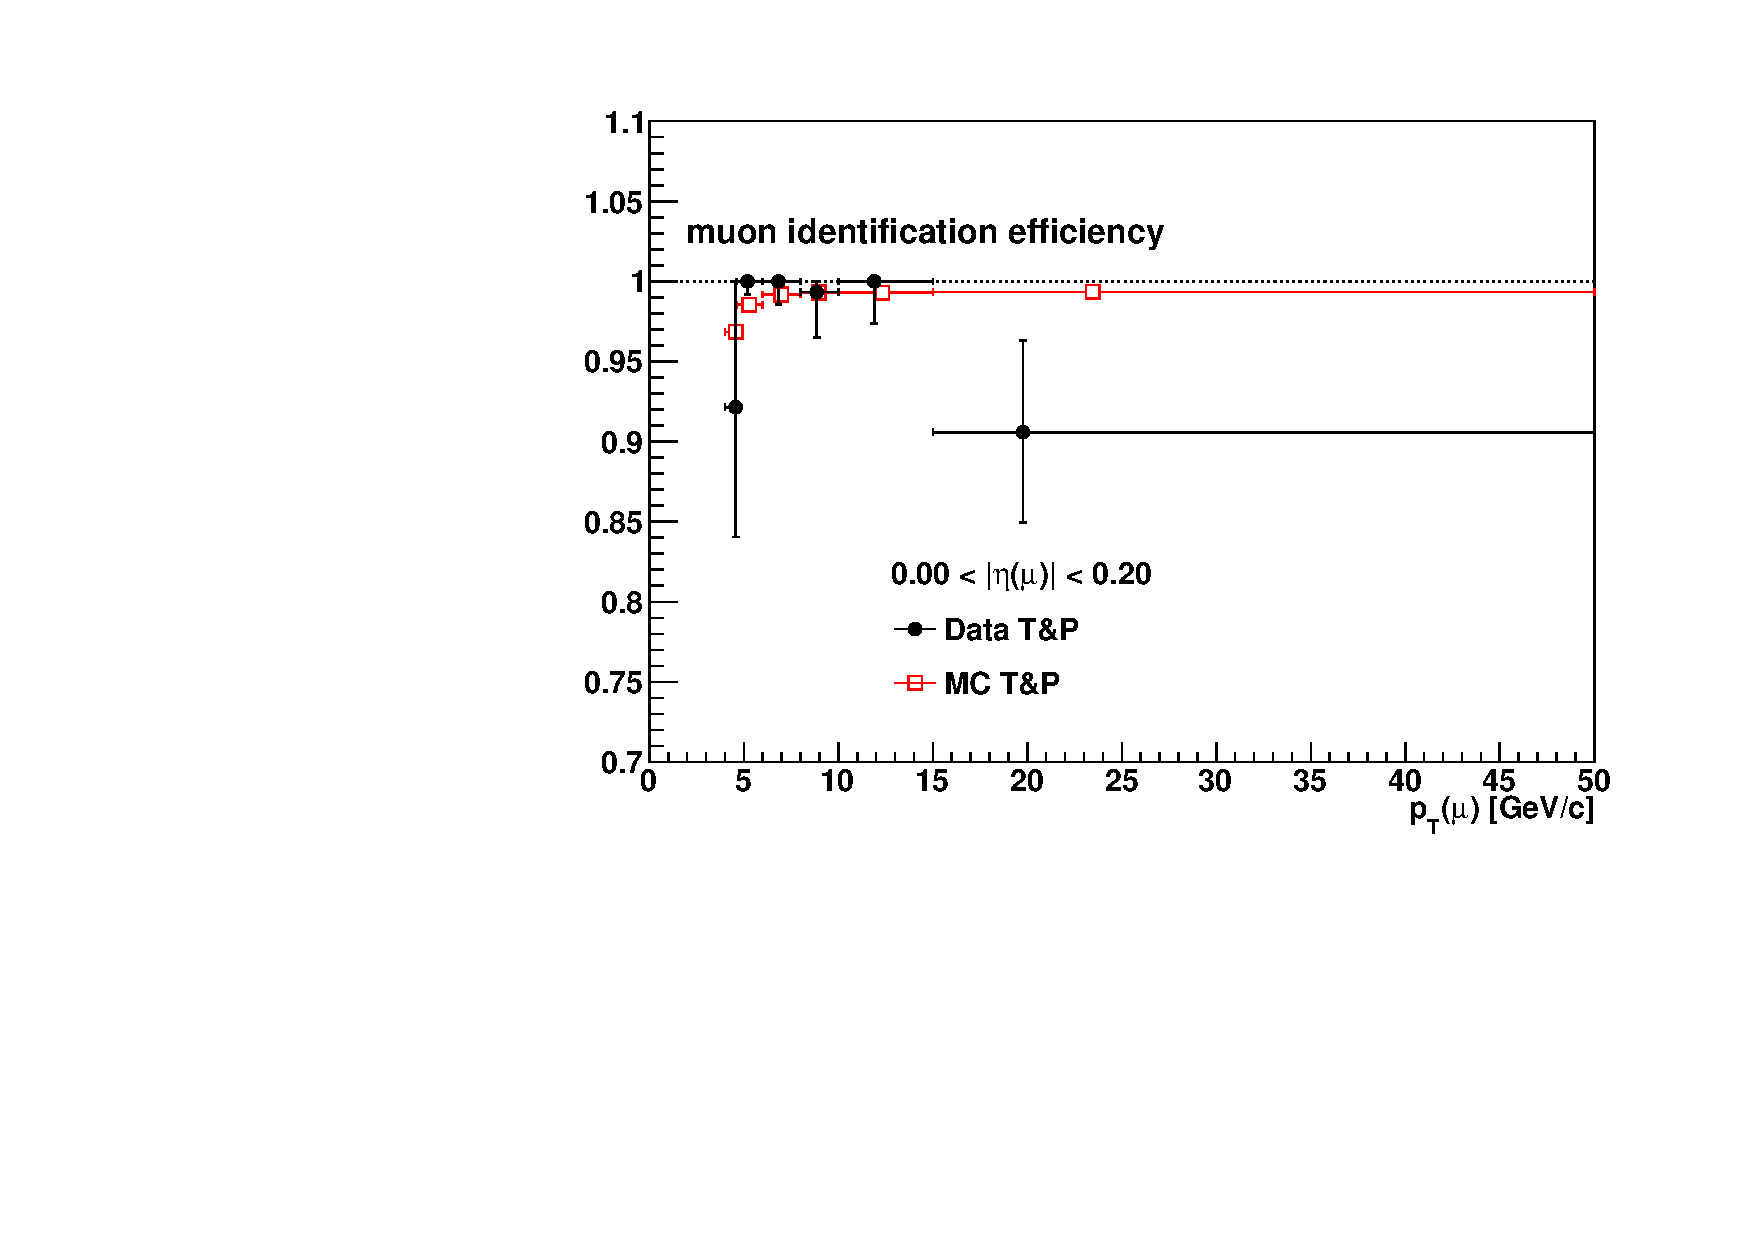
\includegraphics[width=0.49\textwidth]{Figures/\subDirName/MuIDEff_pT_DataVsMC_etaBin0.pdf}
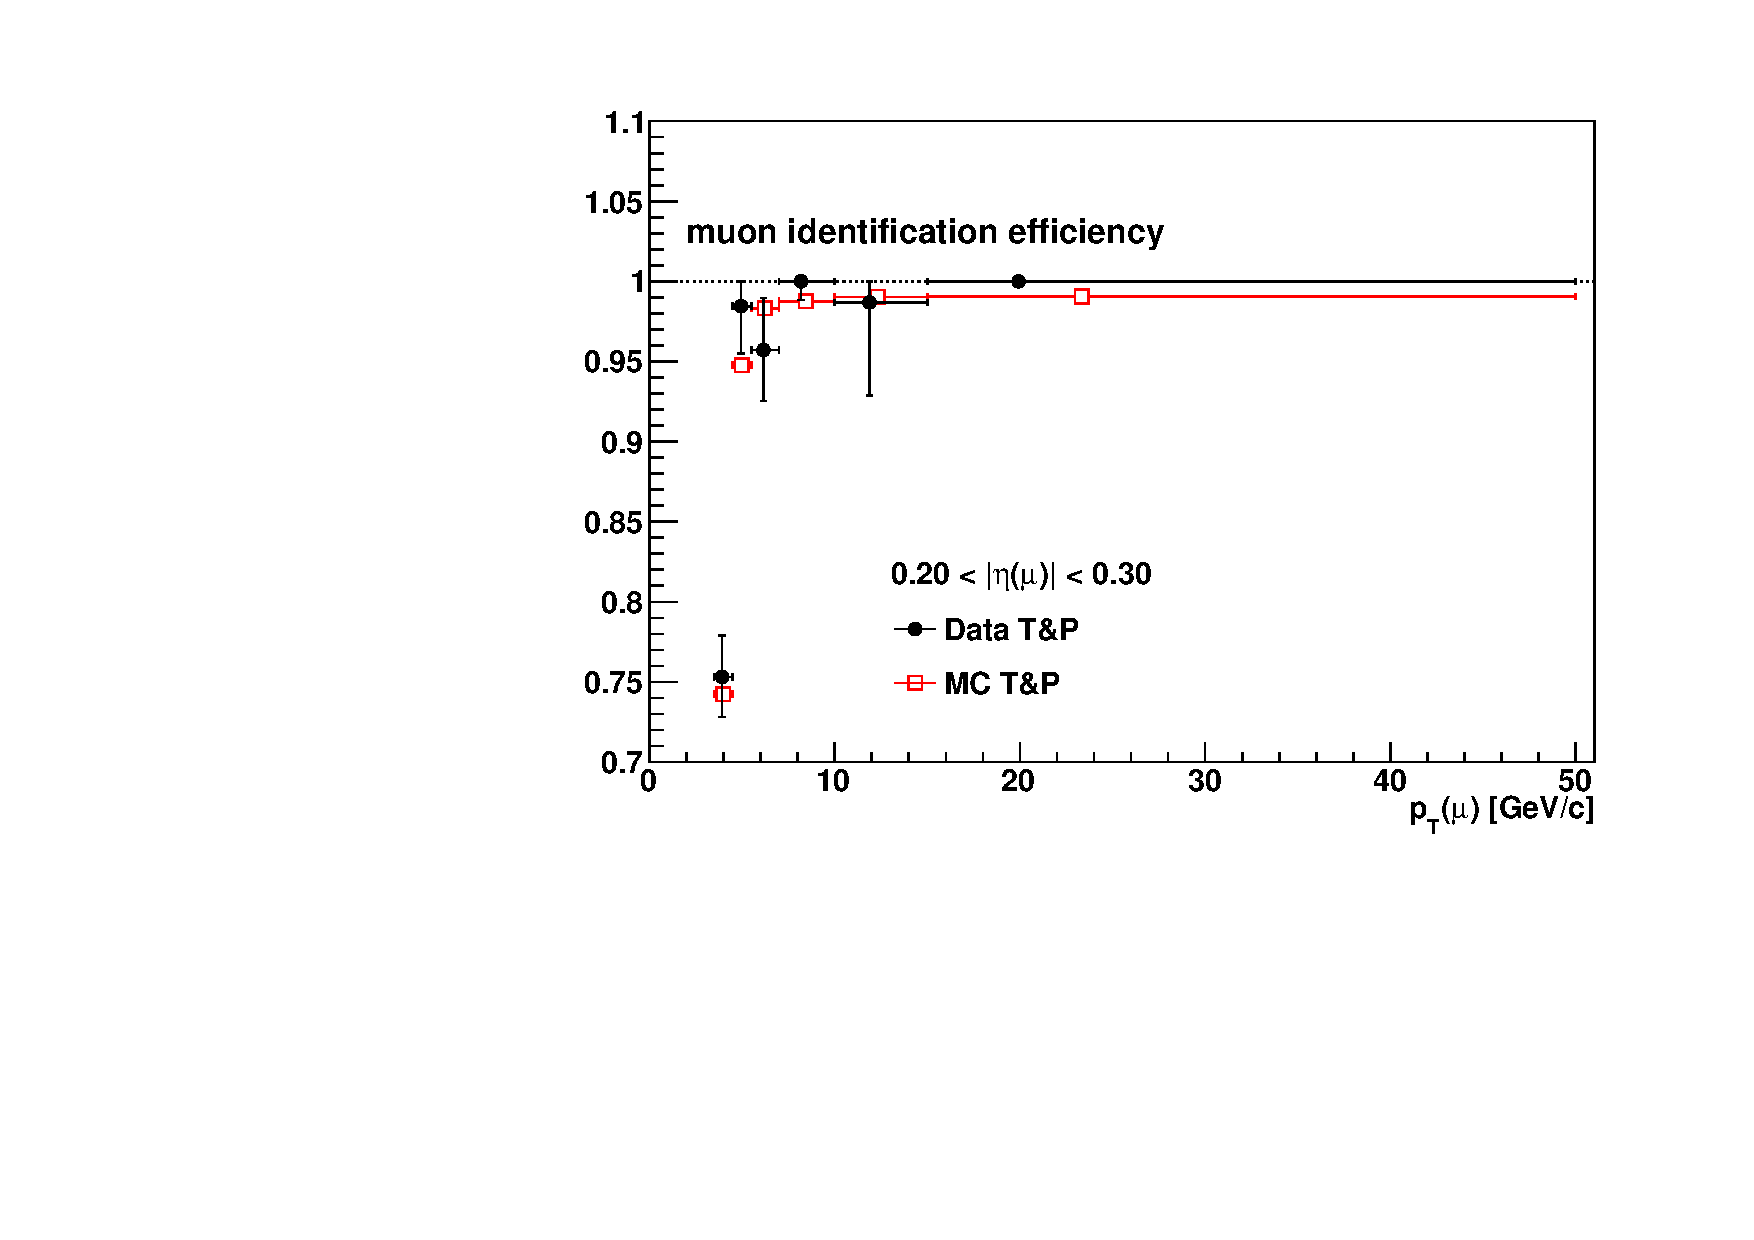
\includegraphics[width=0.49\textwidth]{Figures/\subDirName/MuIDEff_pT_DataVsMC_etaBin1.pdf}
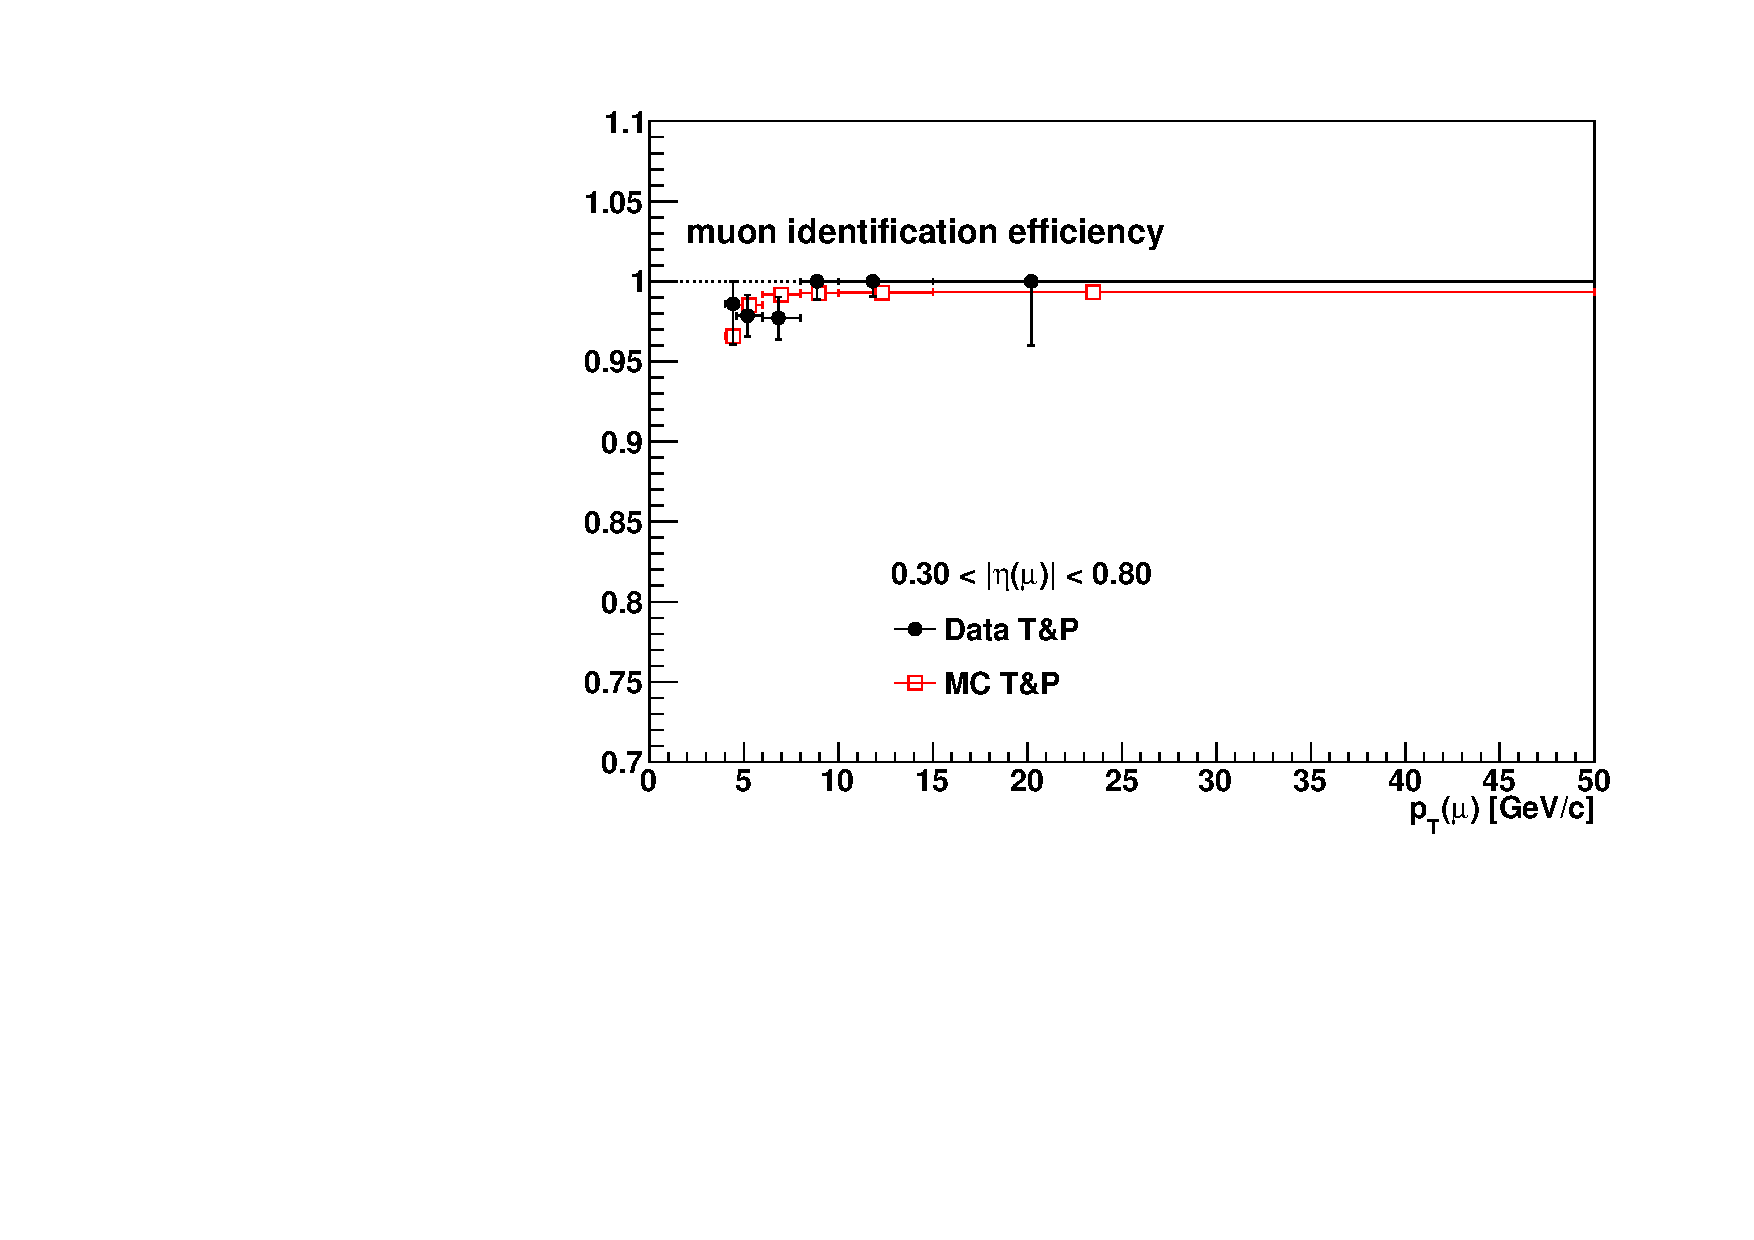
\includegraphics[width=0.49\textwidth]{Figures/\subDirName/MuIDEff_pT_DataVsMC_etaBin2.pdf}
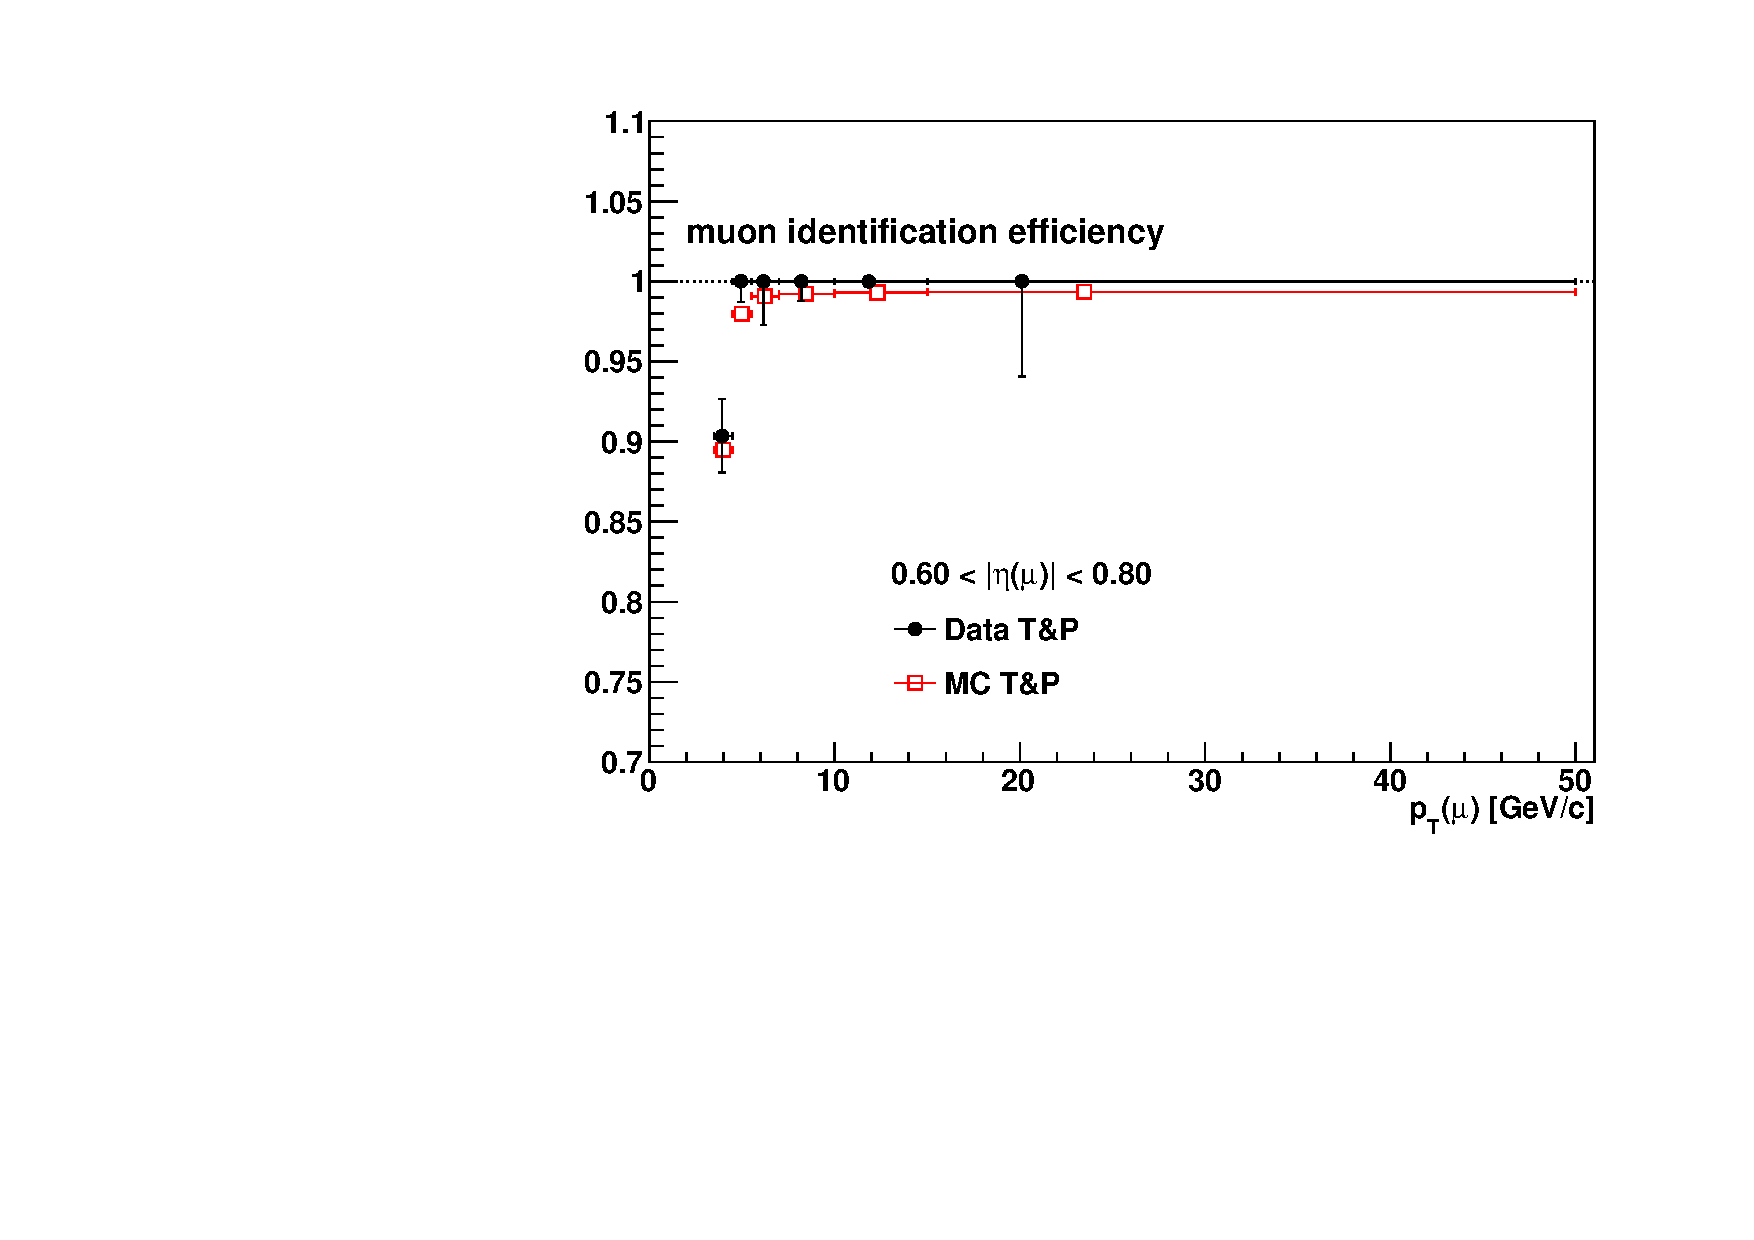
\includegraphics[width=0.49\textwidth]{Figures/\subDirName/MuIDEff_pT_DataVsMC_etaBin3.pdf}
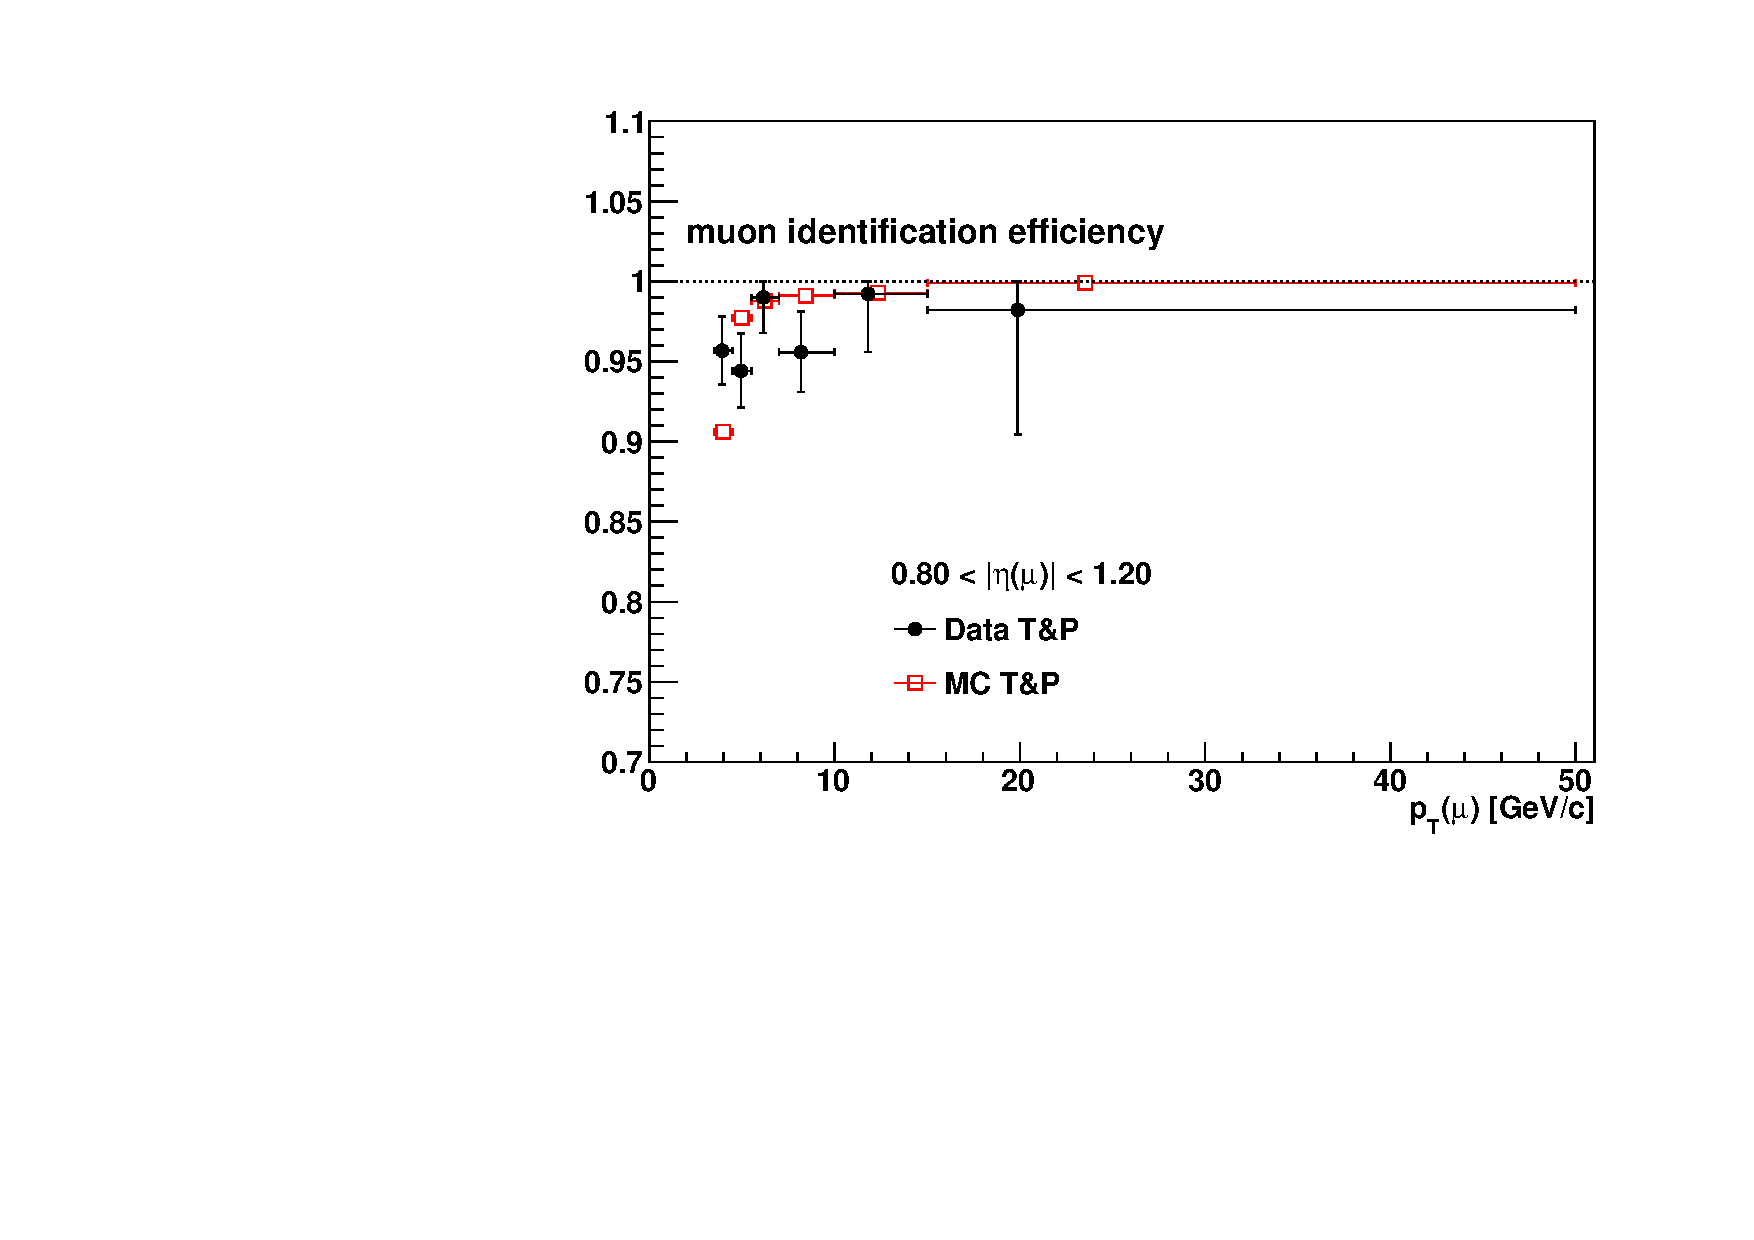
\includegraphics[width=0.49\textwidth]{Figures/\subDirName/MuIDEff_pT_DataVsMC_etaBin4.pdf}
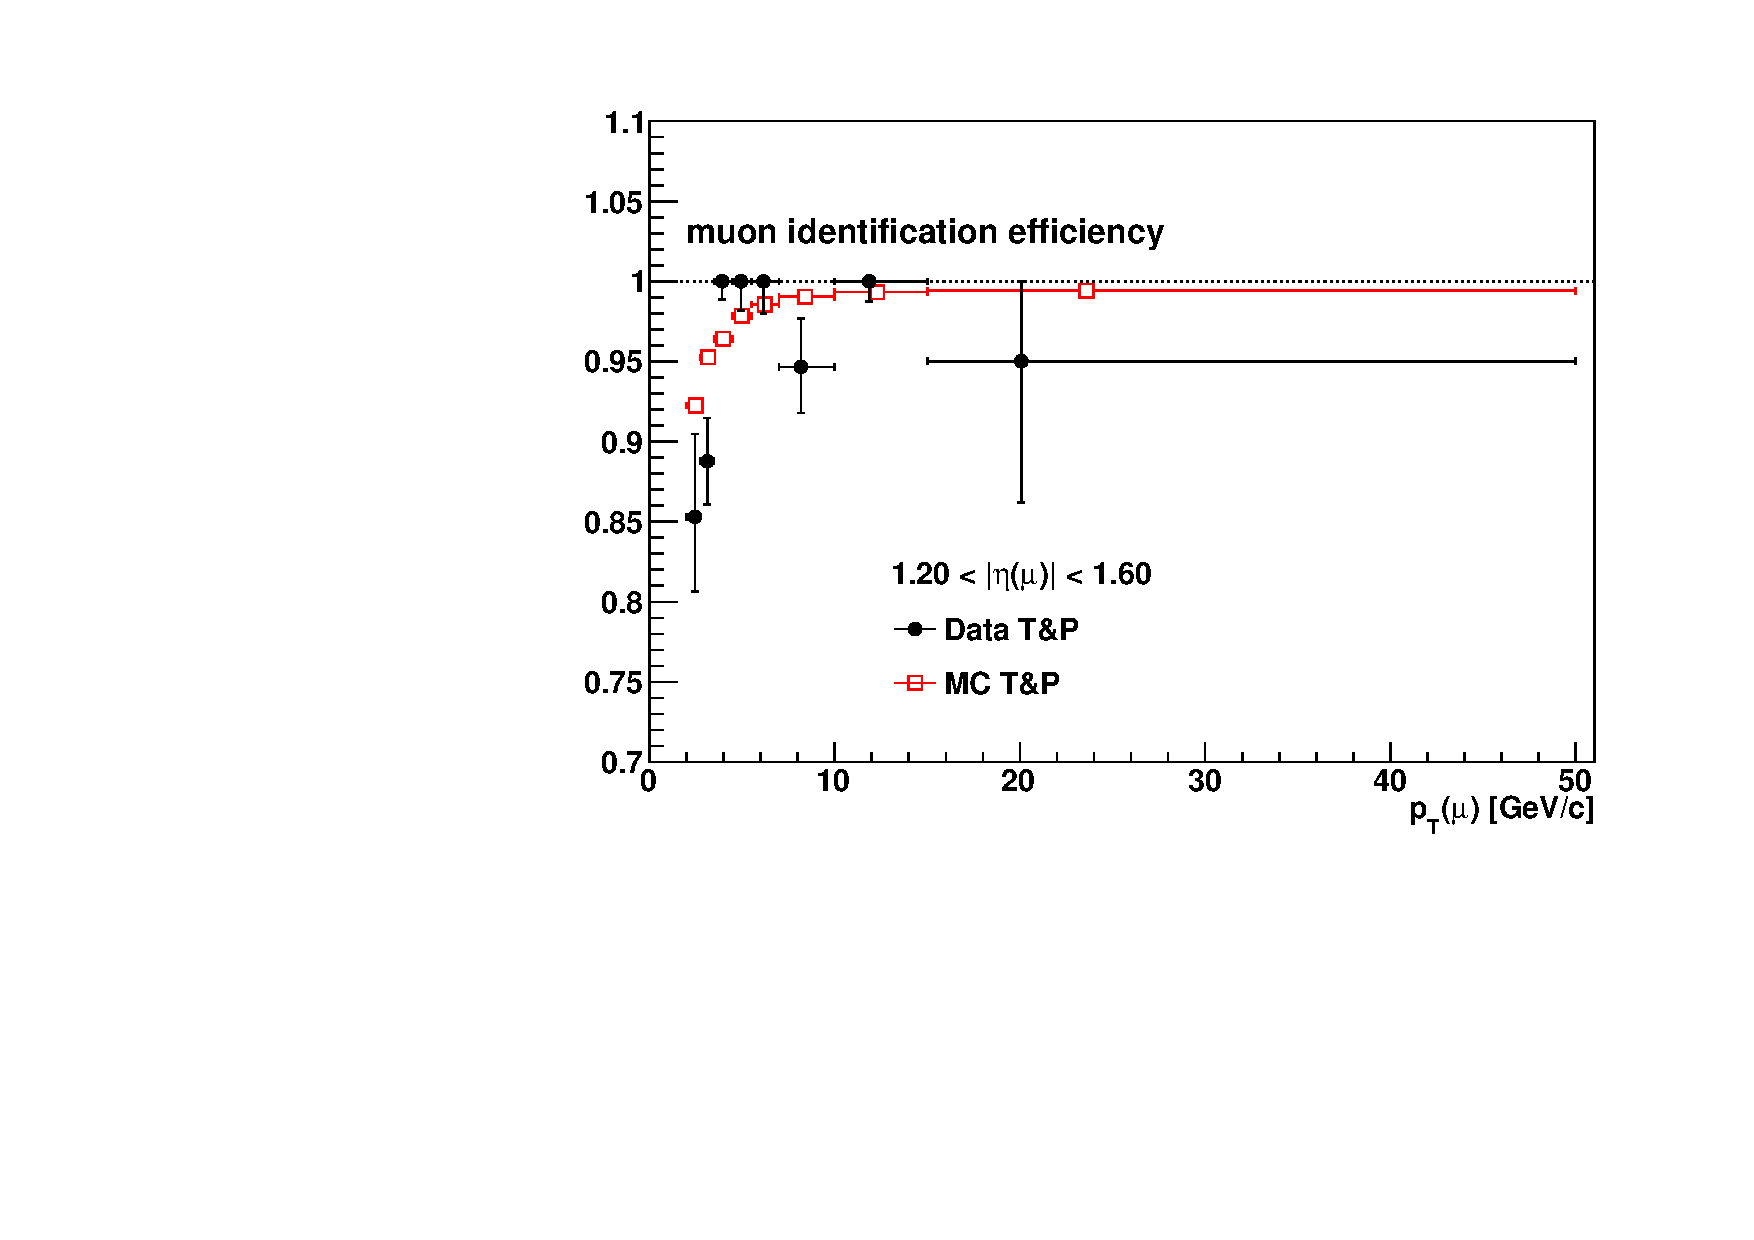
\includegraphics[width=0.49\textwidth]{Figures/\subDirName/MuIDEff_pT_DataVsMC_etaBin5.pdf}
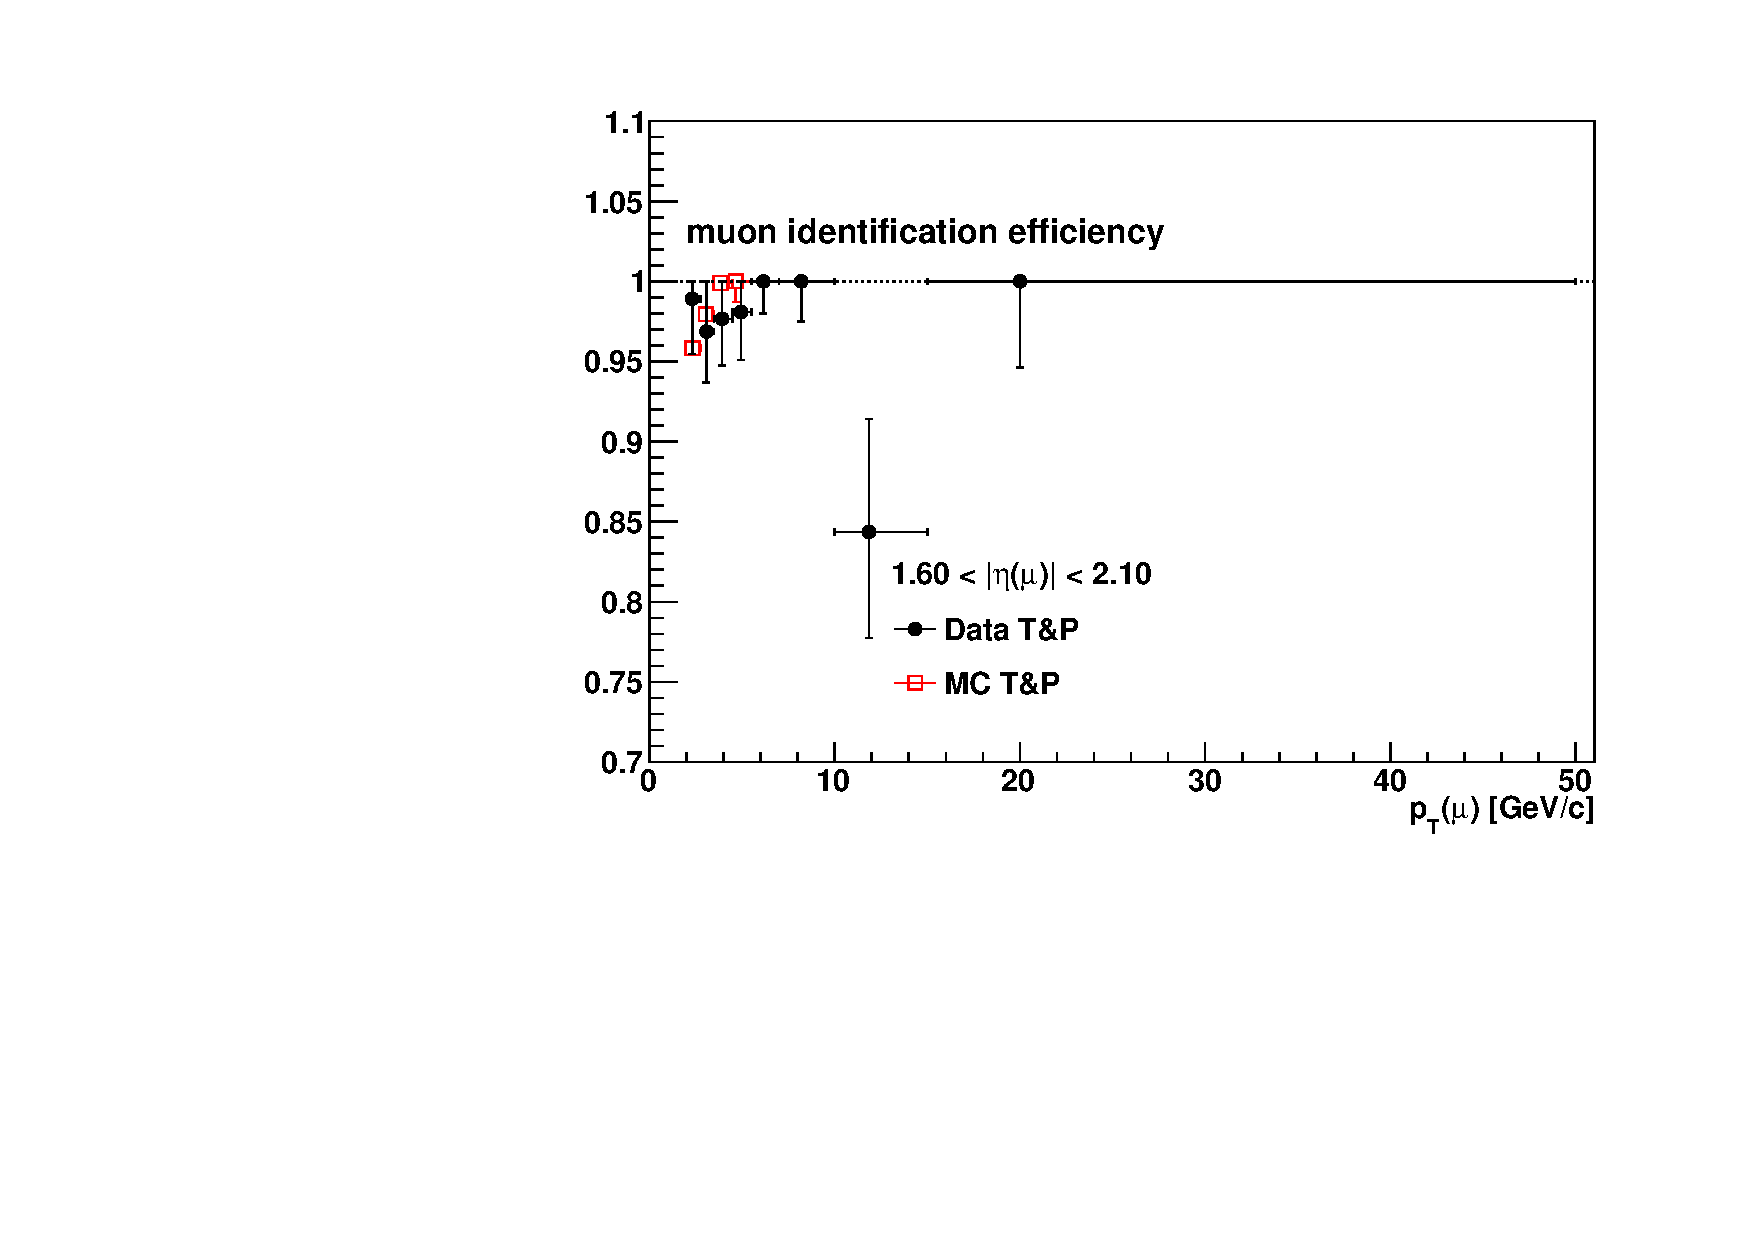
\includegraphics[width=0.49\textwidth]{Figures/\subDirName/MuIDEff_pT_DataVsMC_etaBin6.pdf}
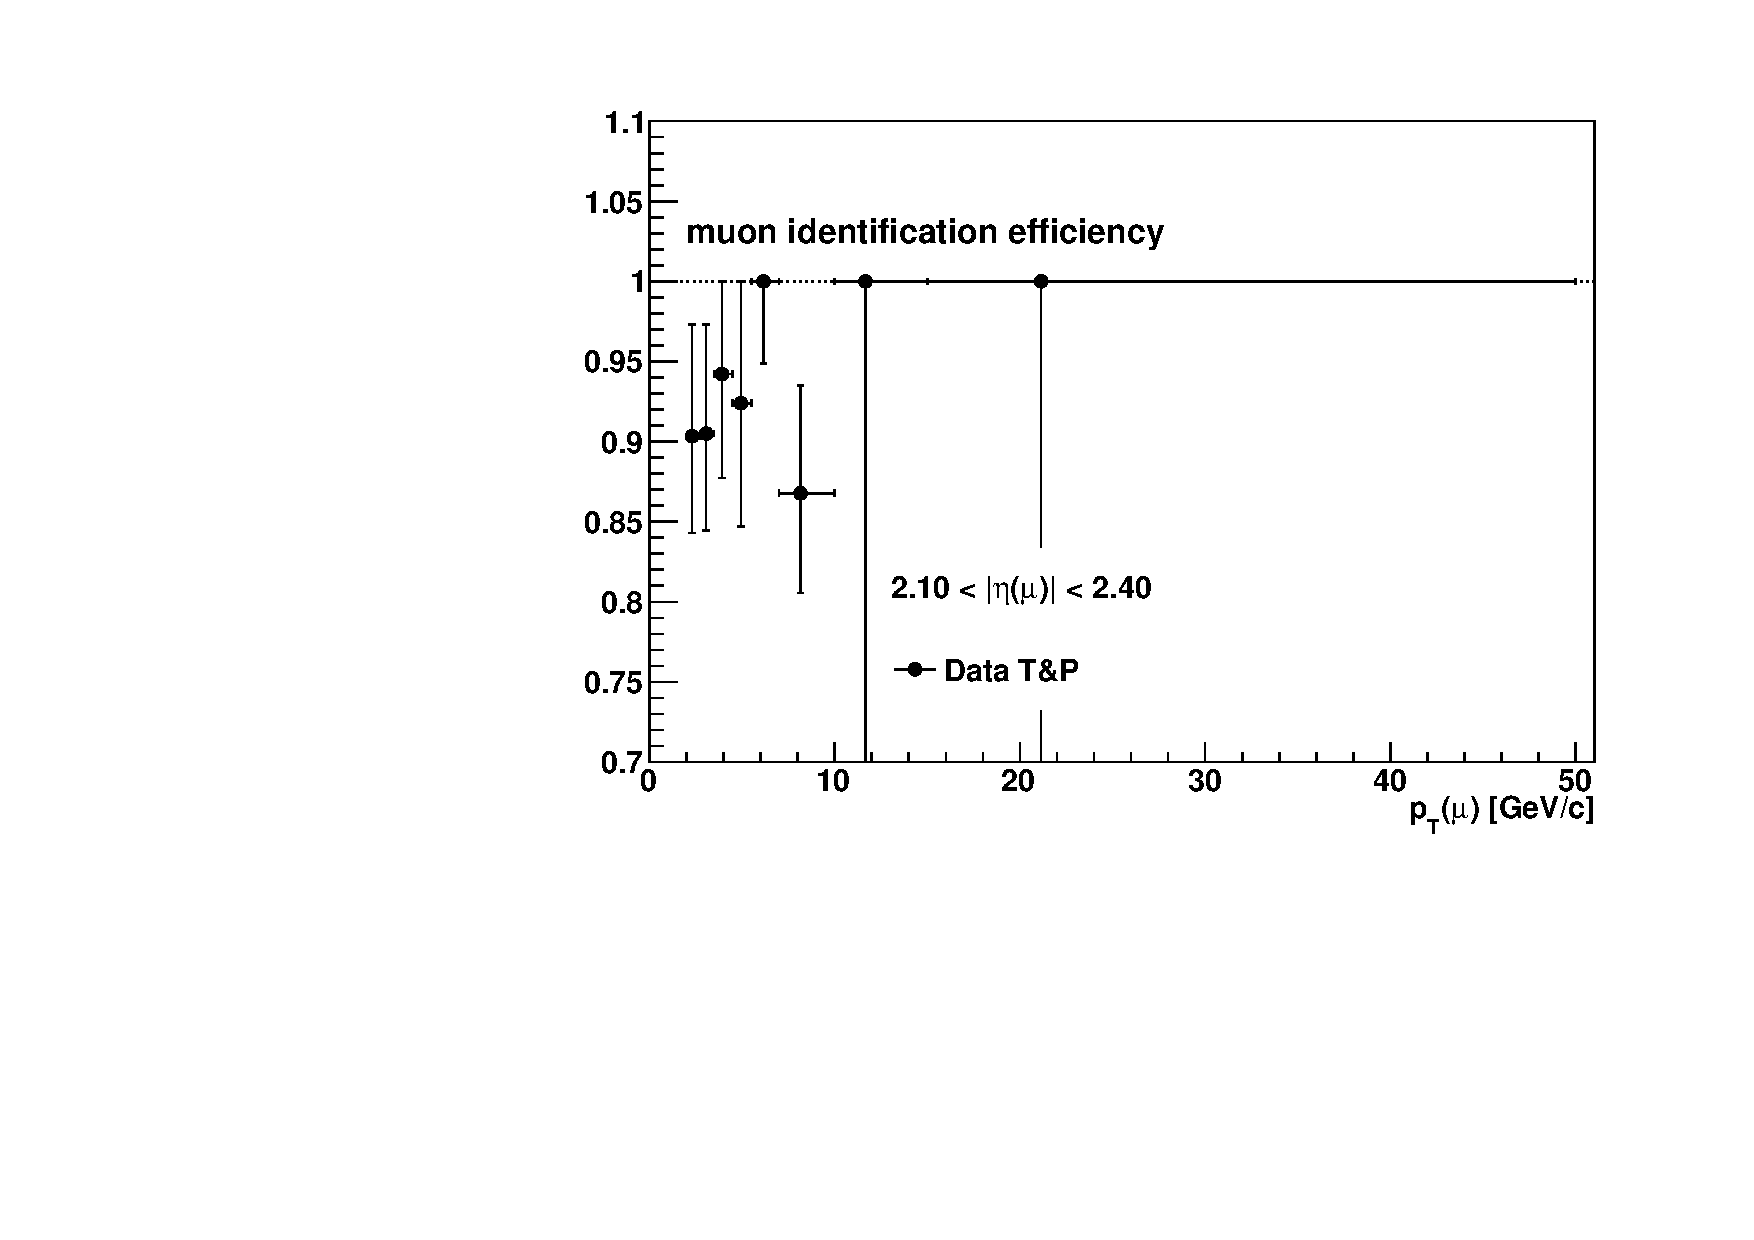
\includegraphics[width=0.49\textwidth]{Figures/\subDirName/MuIDEff_pT_DataVsMC_etaBin7.pdf}
\caption{Muon reconstruction efficiency versus \pt\ for small slices
  in $|\eta|$, using the ``tracker50'' muon cuts.}
\label{fig:muonIDEff-pt}
\end{figure}
\begin{figure}[p]
\centering
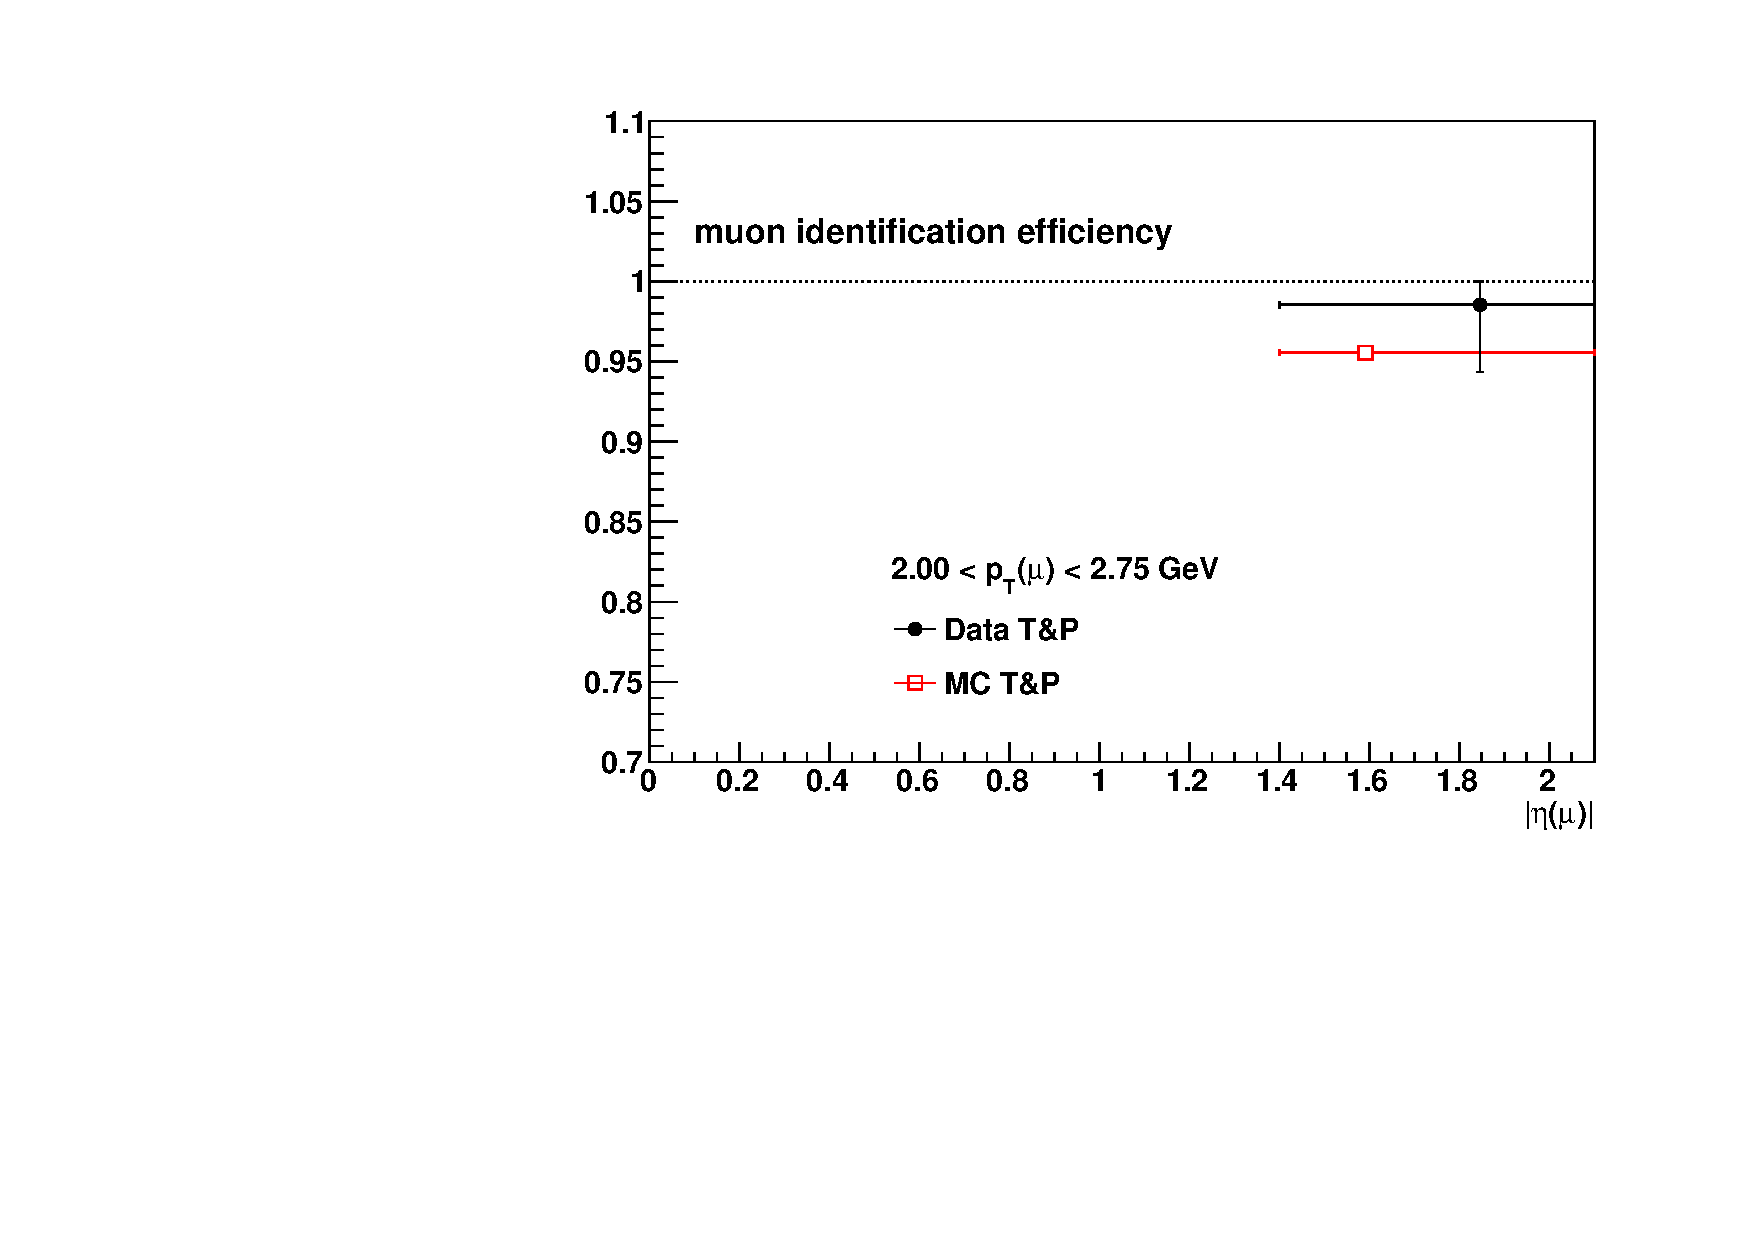
\includegraphics[width=0.49\textwidth]{Figures/\subDirName/MuIDEff_eta_DataVsMC_pTBin0.pdf}
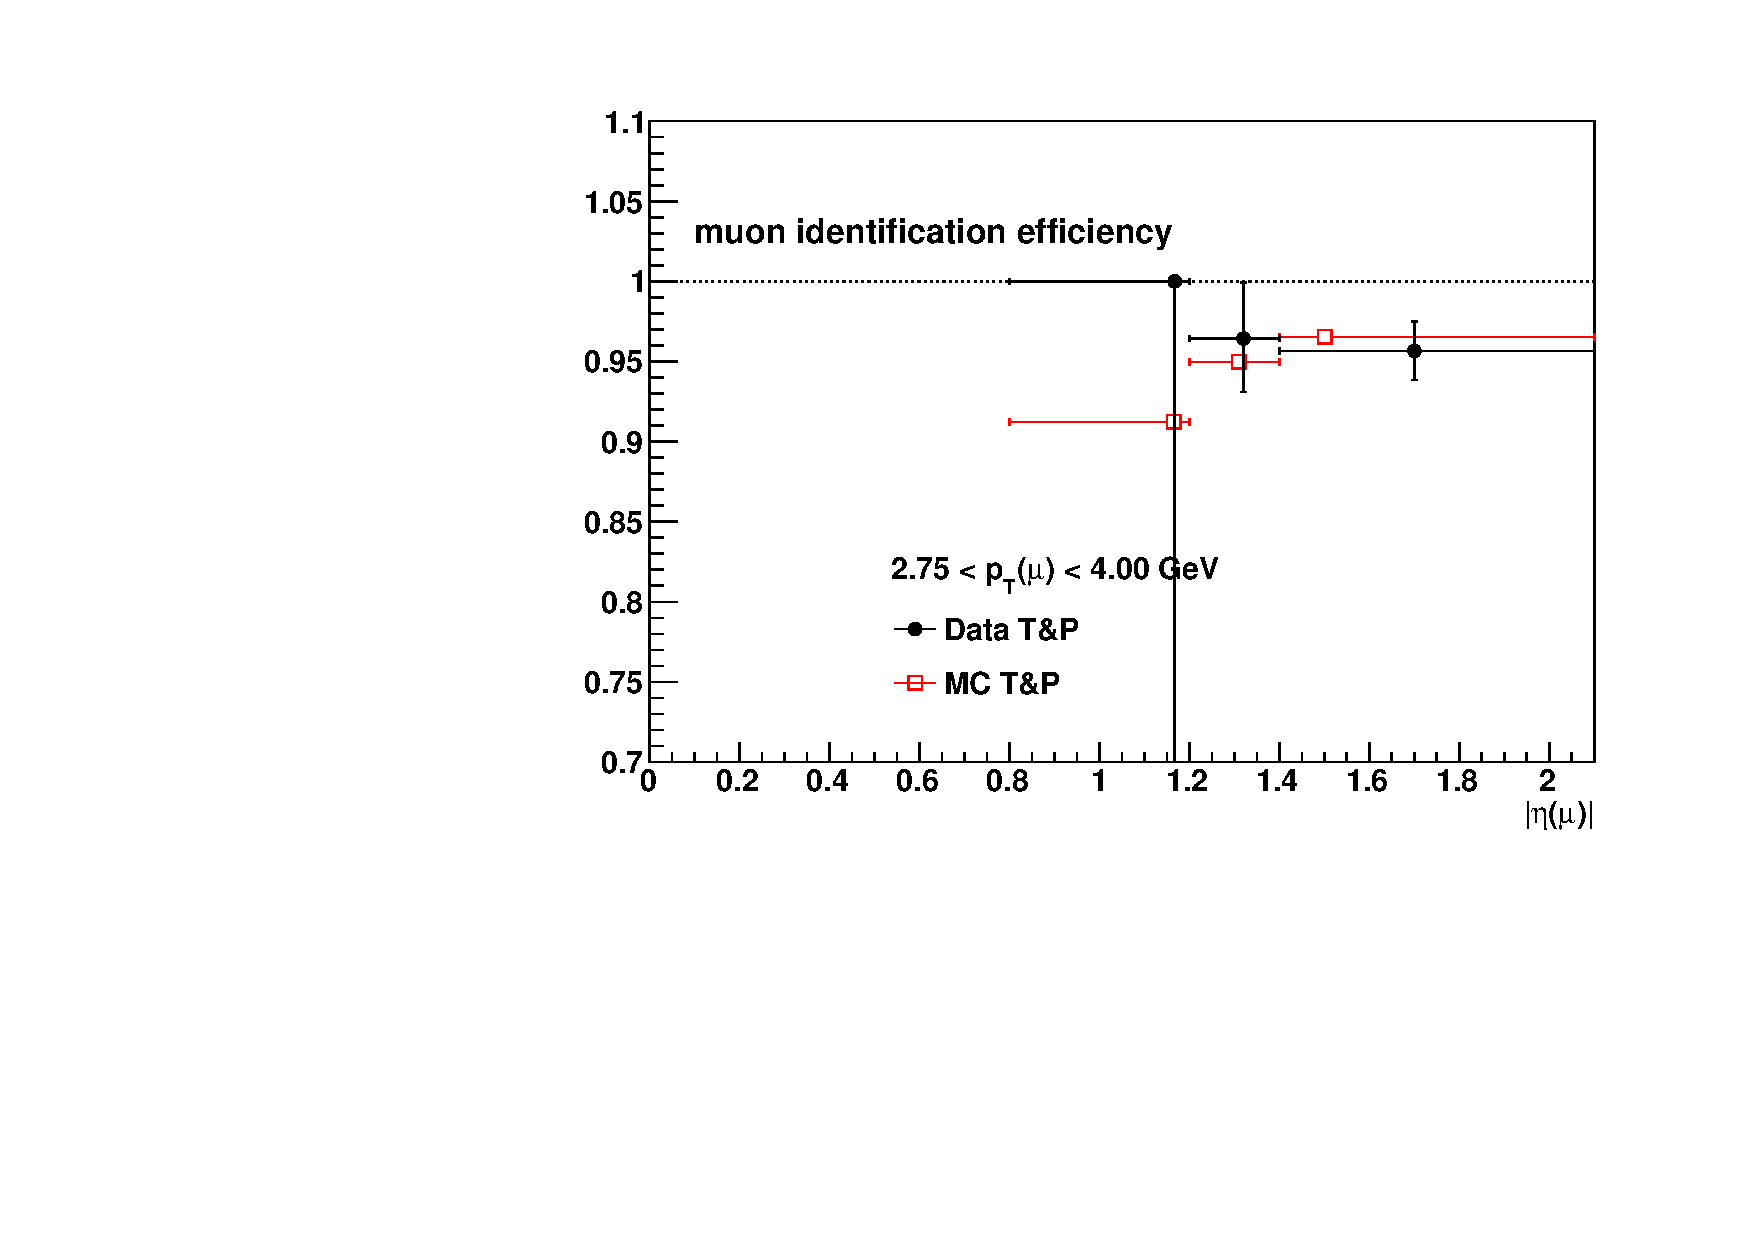
\includegraphics[width=0.49\textwidth]{Figures/\subDirName/MuIDEff_eta_DataVsMC_pTBin1.pdf}
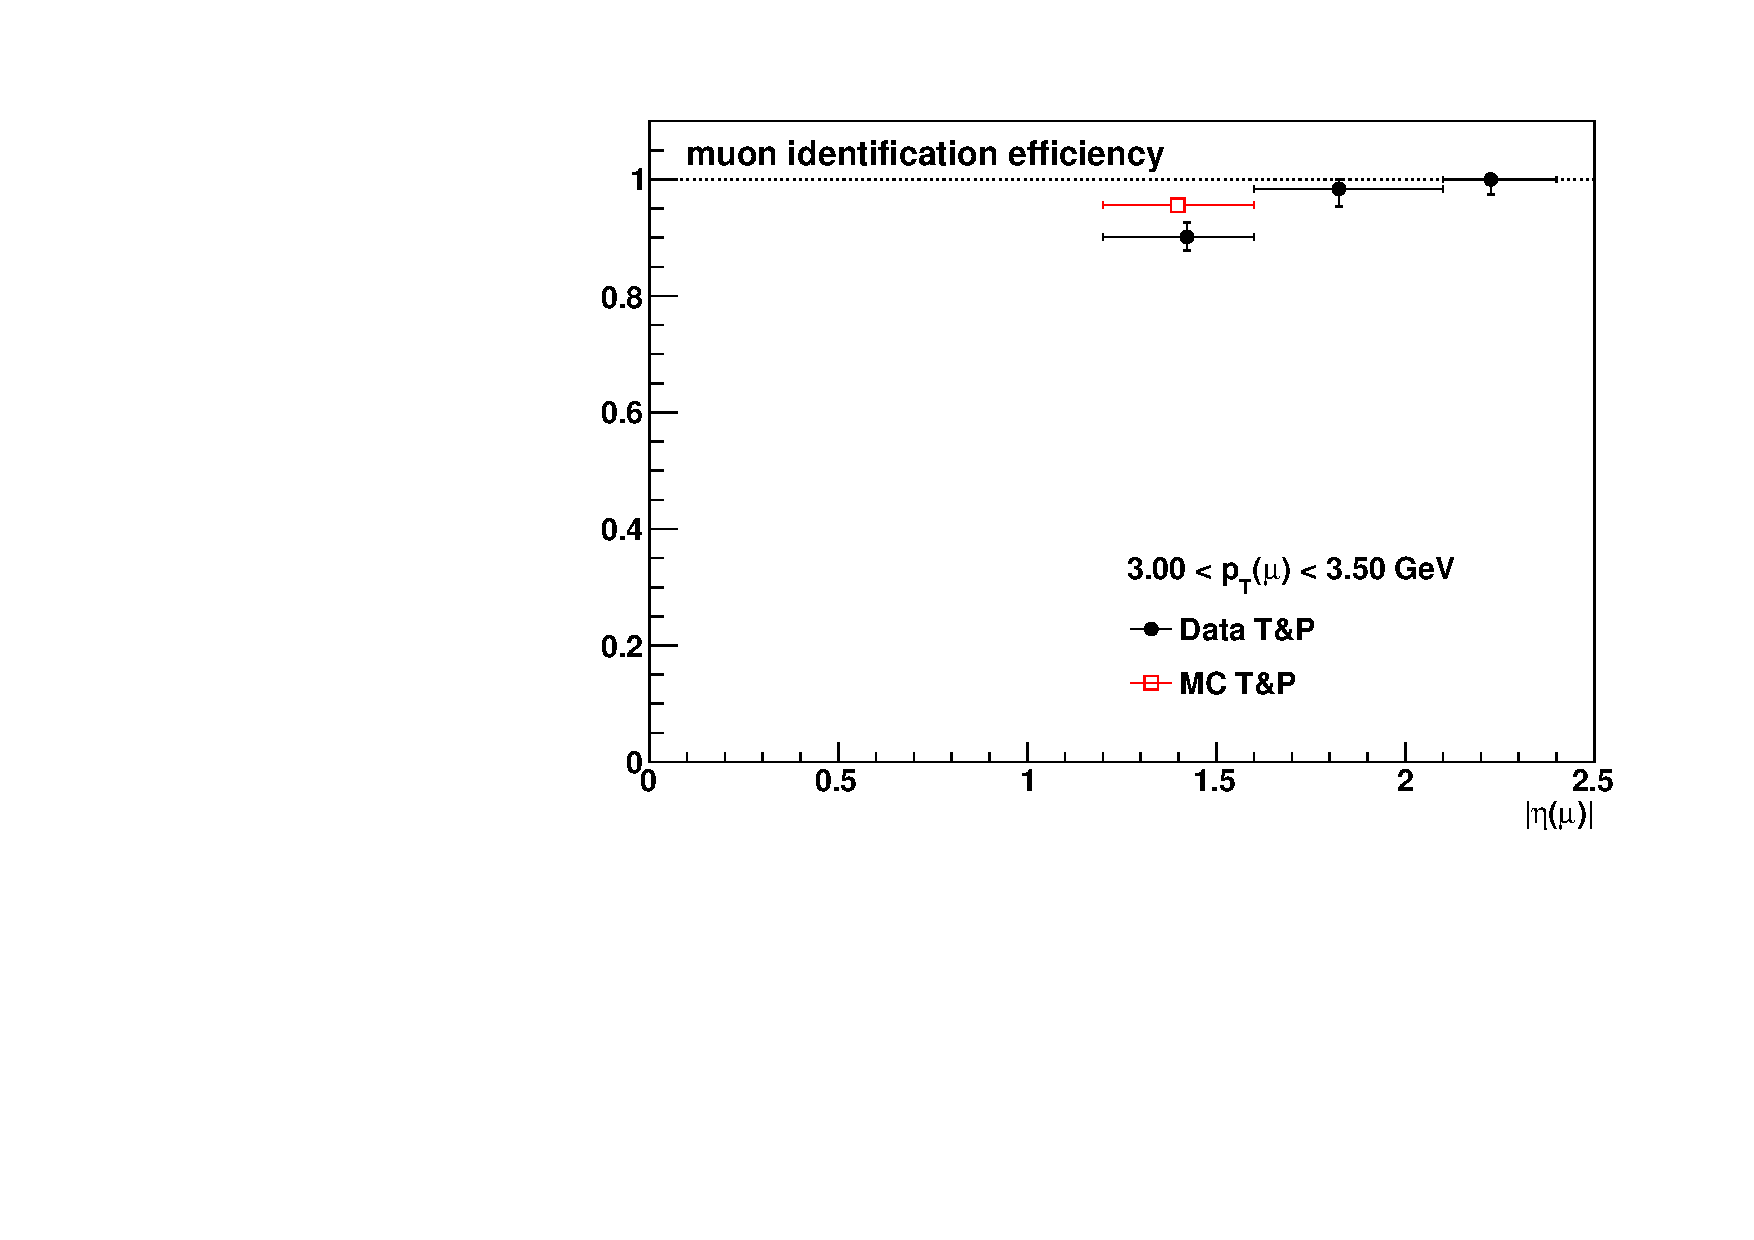
\includegraphics[width=0.49\textwidth]{Figures/\subDirName/MuIDEff_eta_DataVsMC_pTBin2.pdf}
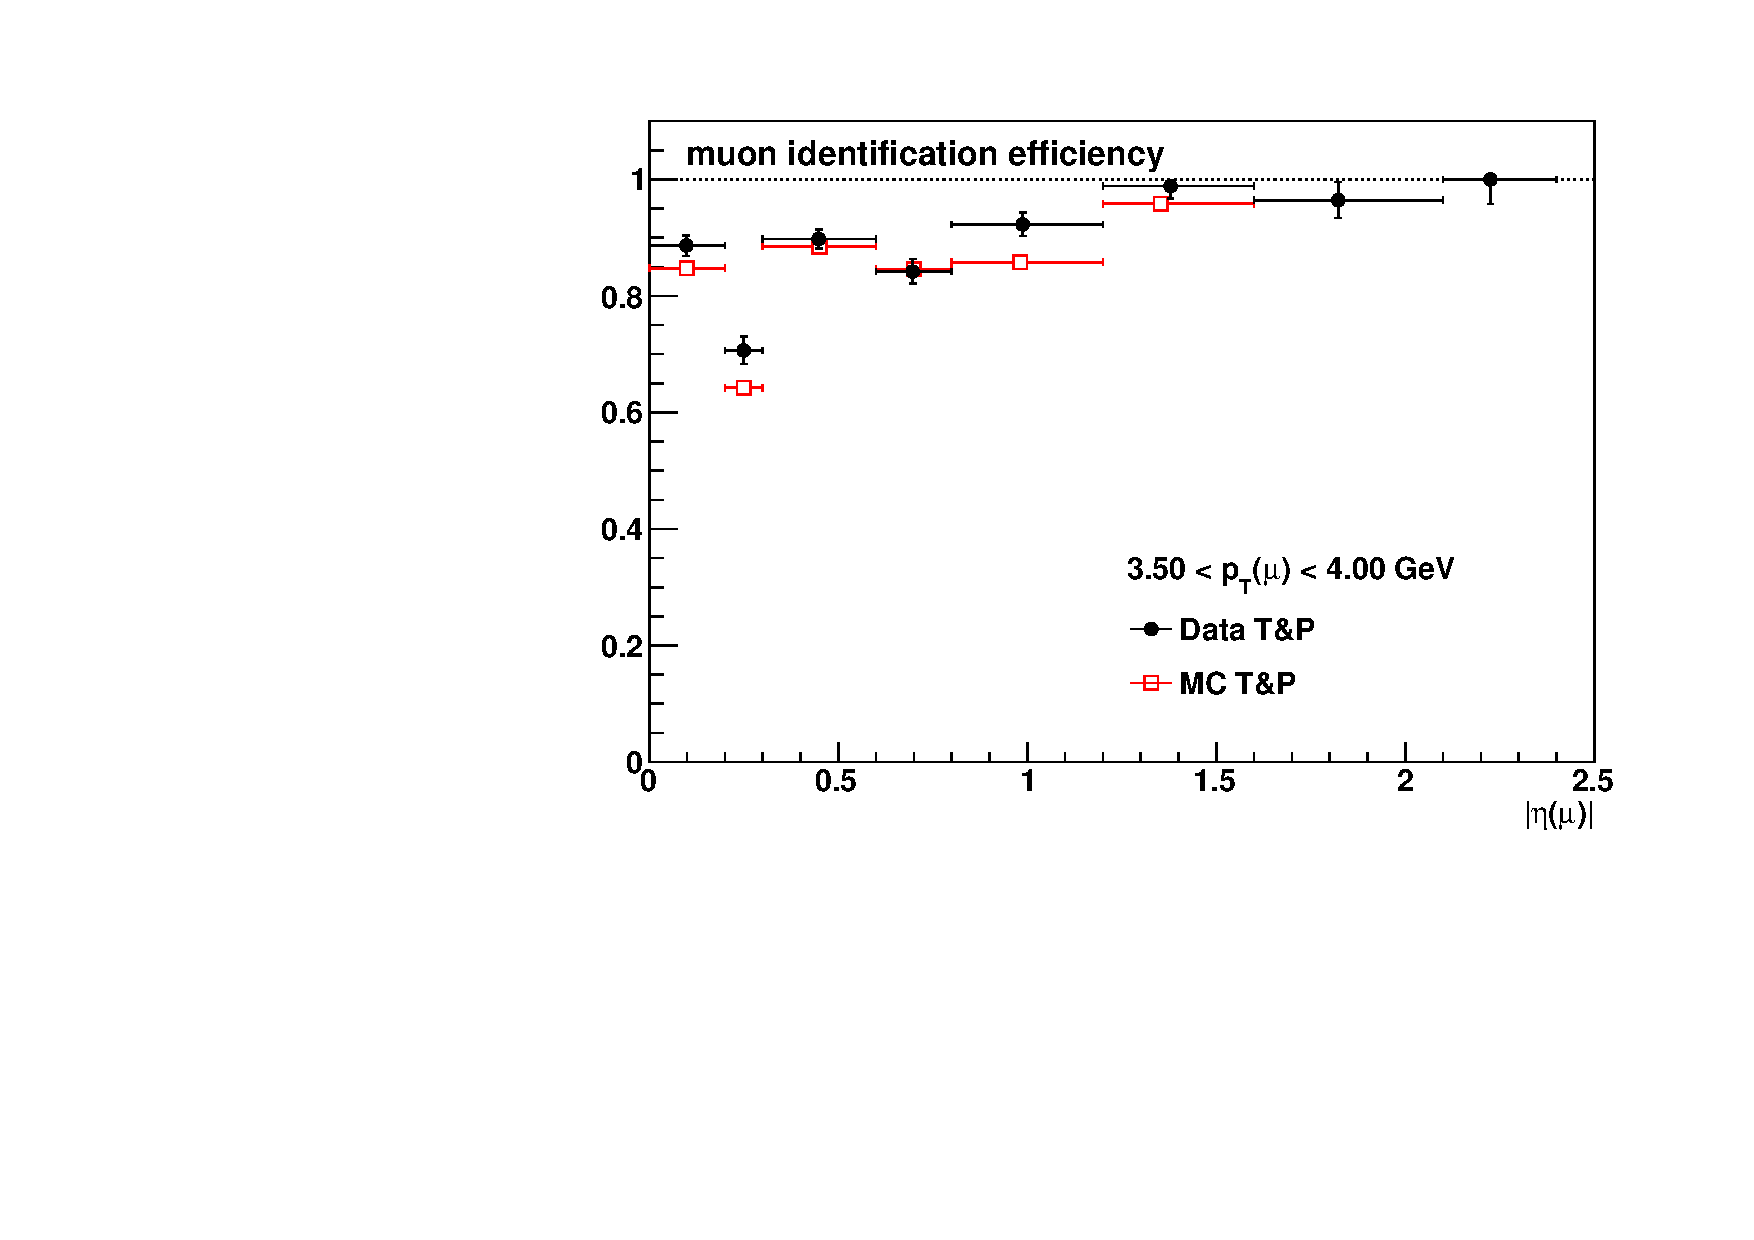
\includegraphics[width=0.49\textwidth]{Figures/\subDirName/MuIDEff_eta_DataVsMC_pTBin3.pdf}
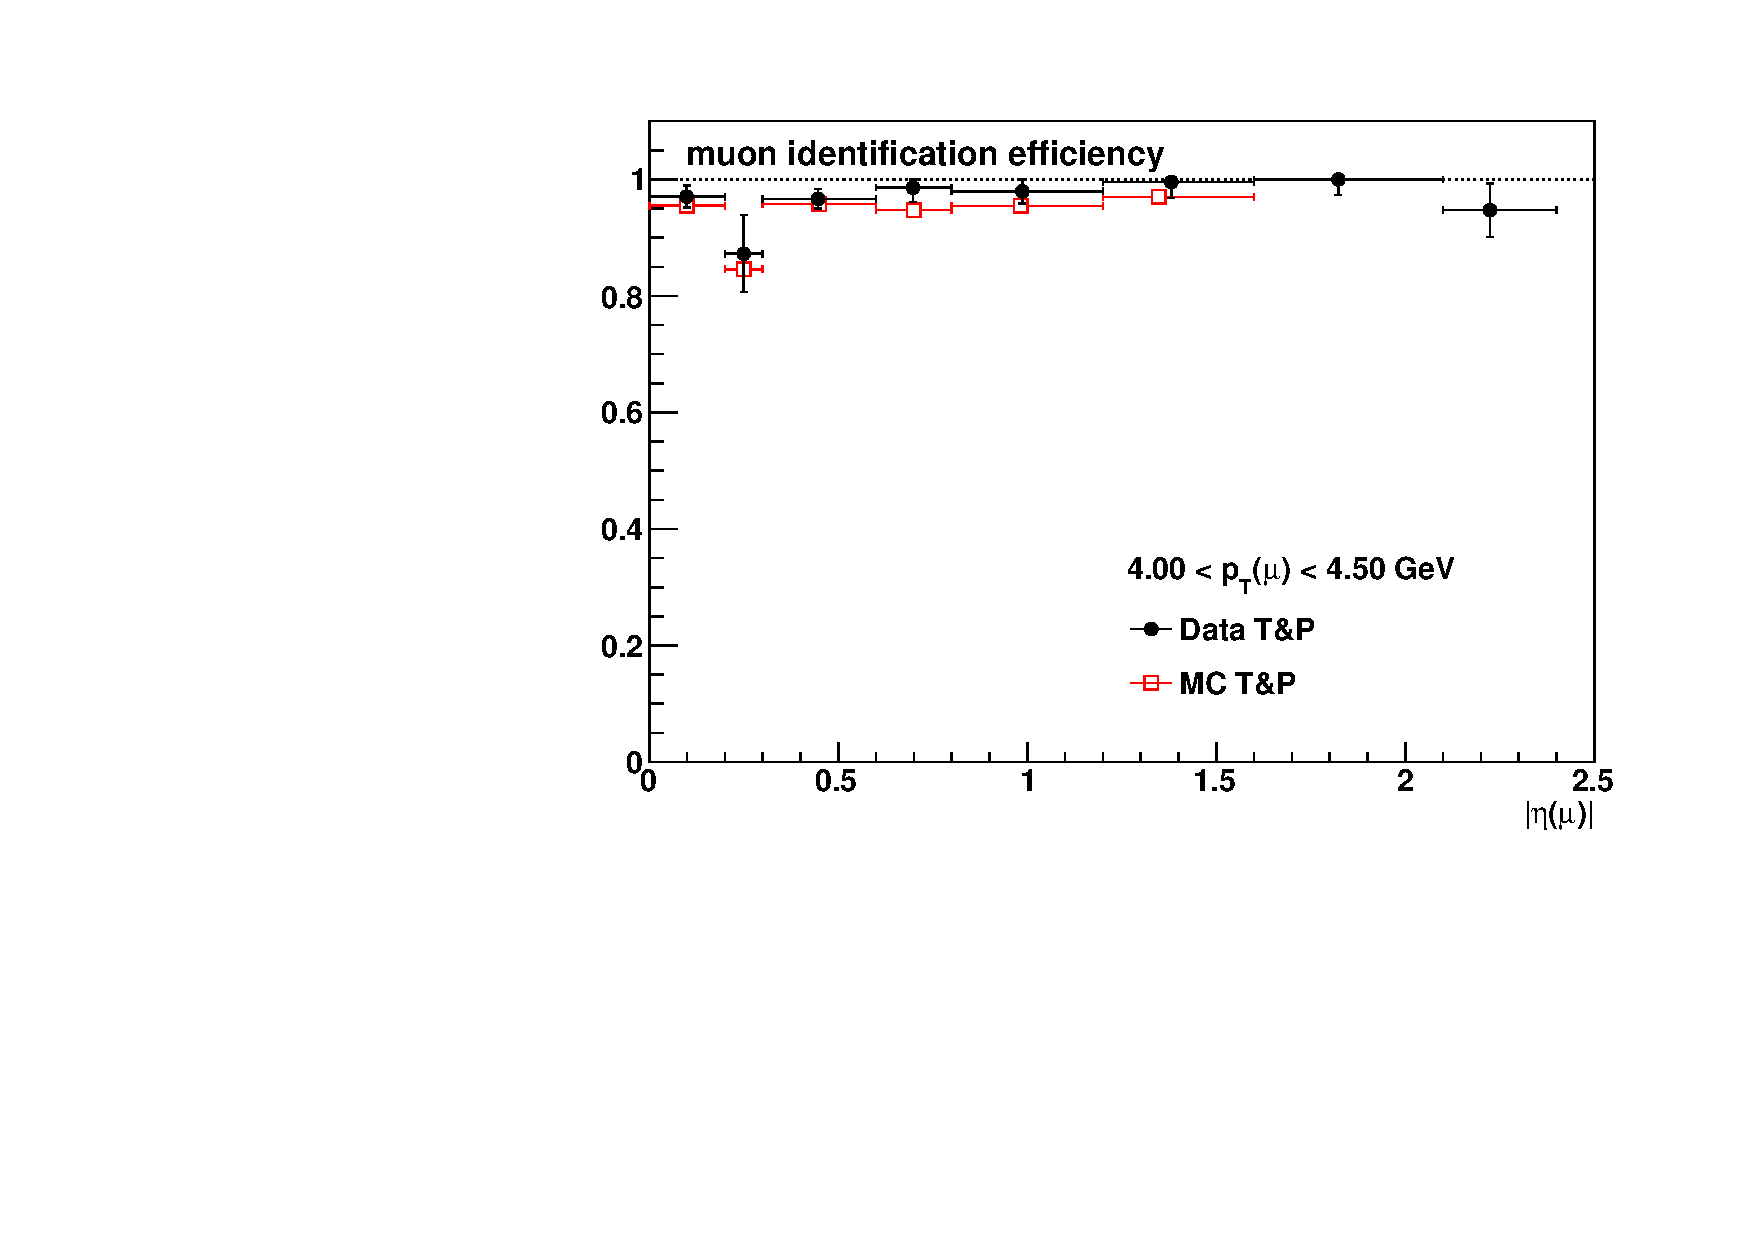
\includegraphics[width=0.49\textwidth]{Figures/\subDirName/MuIDEff_eta_DataVsMC_pTBin4.pdf}
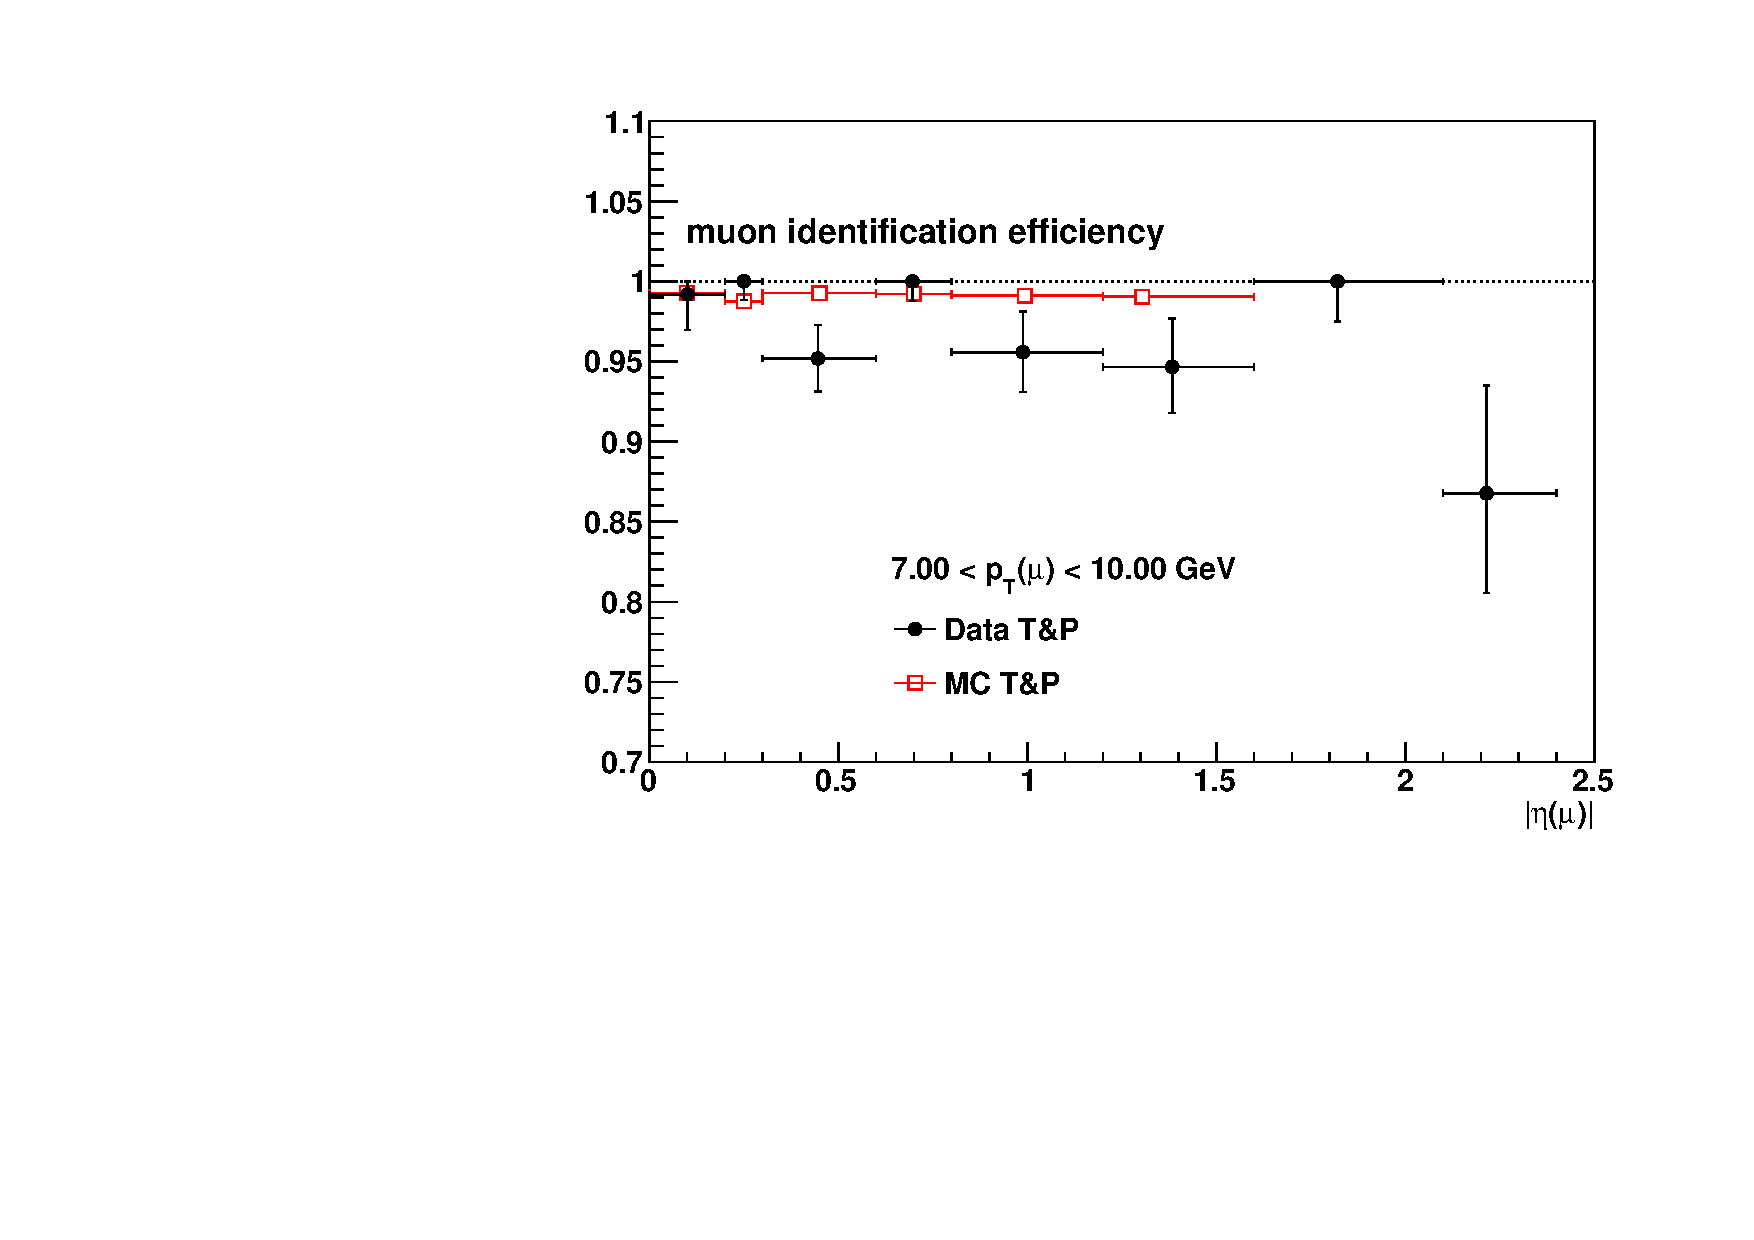
\includegraphics[width=0.49\textwidth]{Figures/\subDirName/MuIDEff_eta_DataVsMC_pTBin5.pdf}
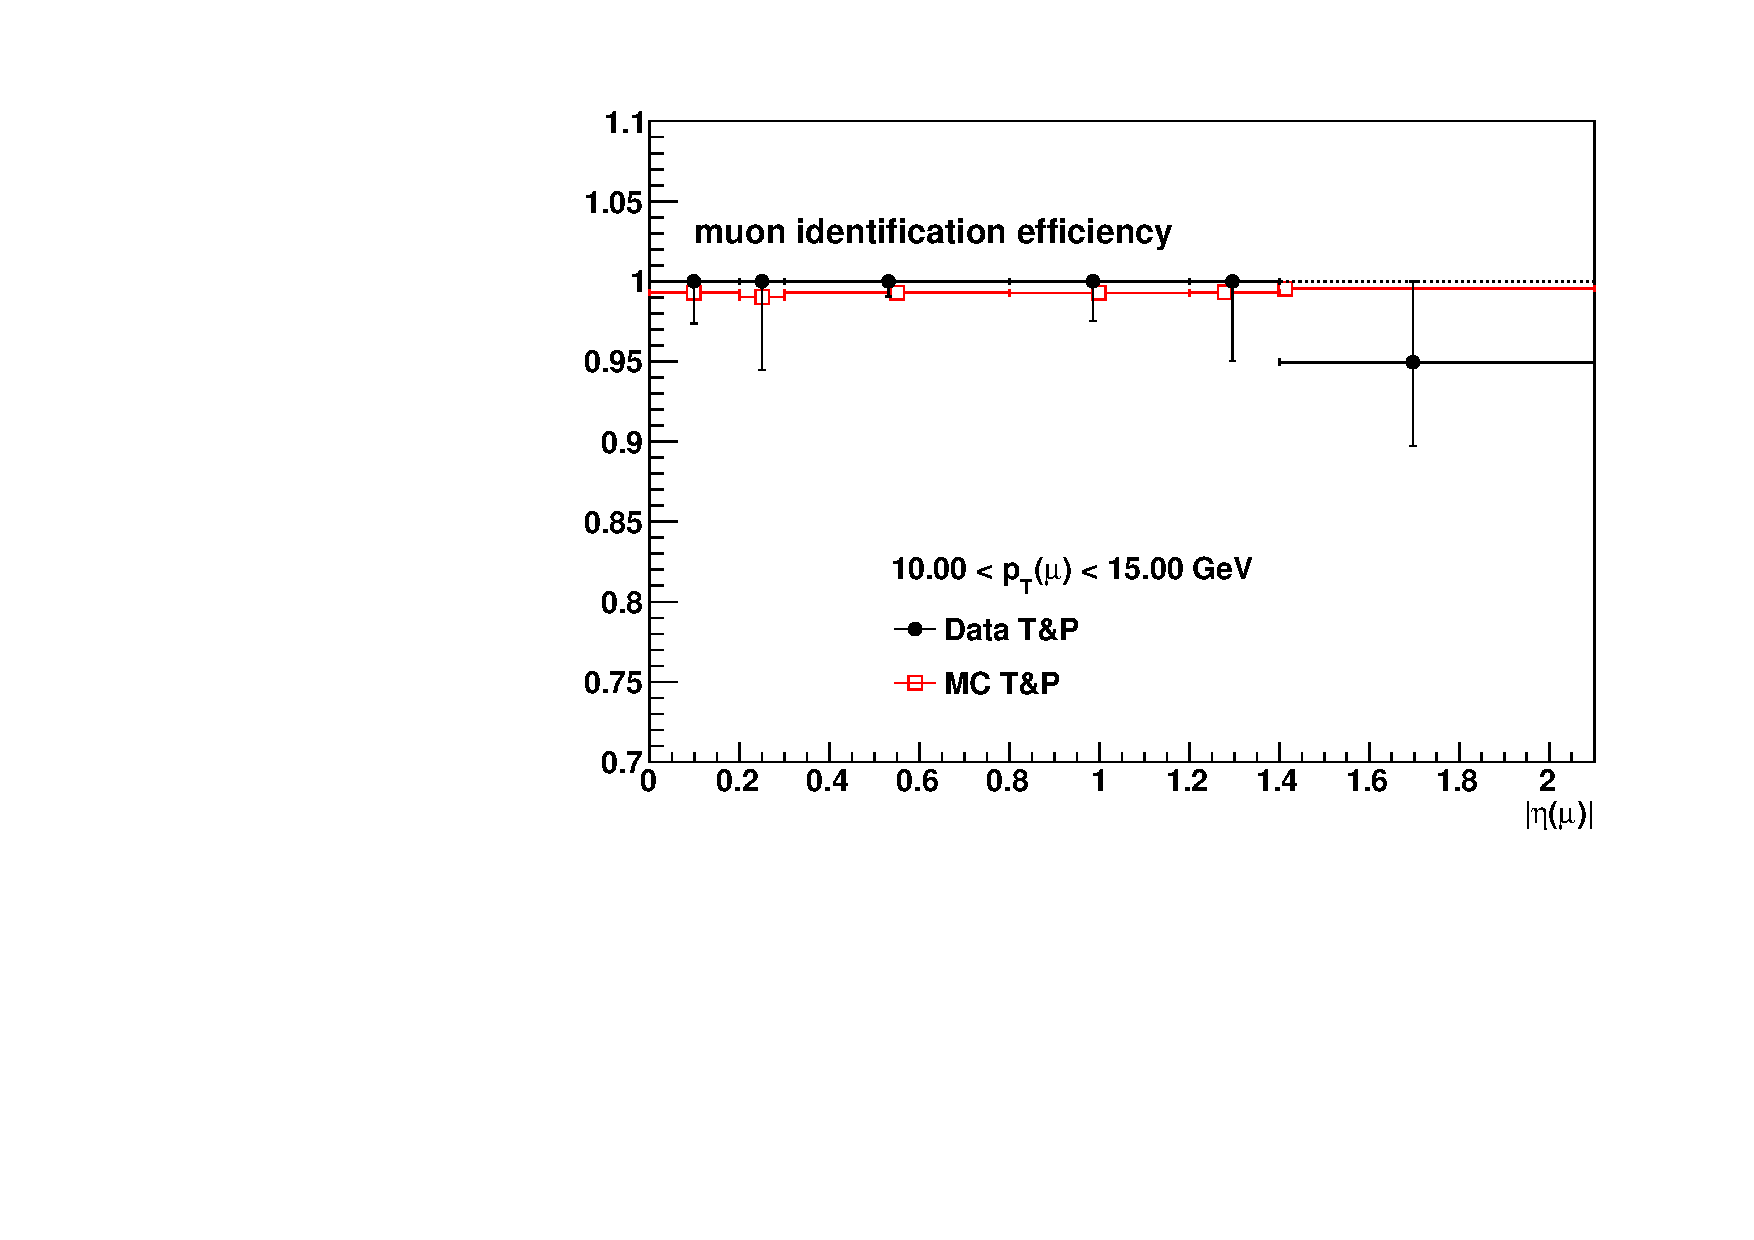
\includegraphics[width=0.49\textwidth]{Figures/\subDirName/MuIDEff_eta_DataVsMC_pTBin6.pdf}
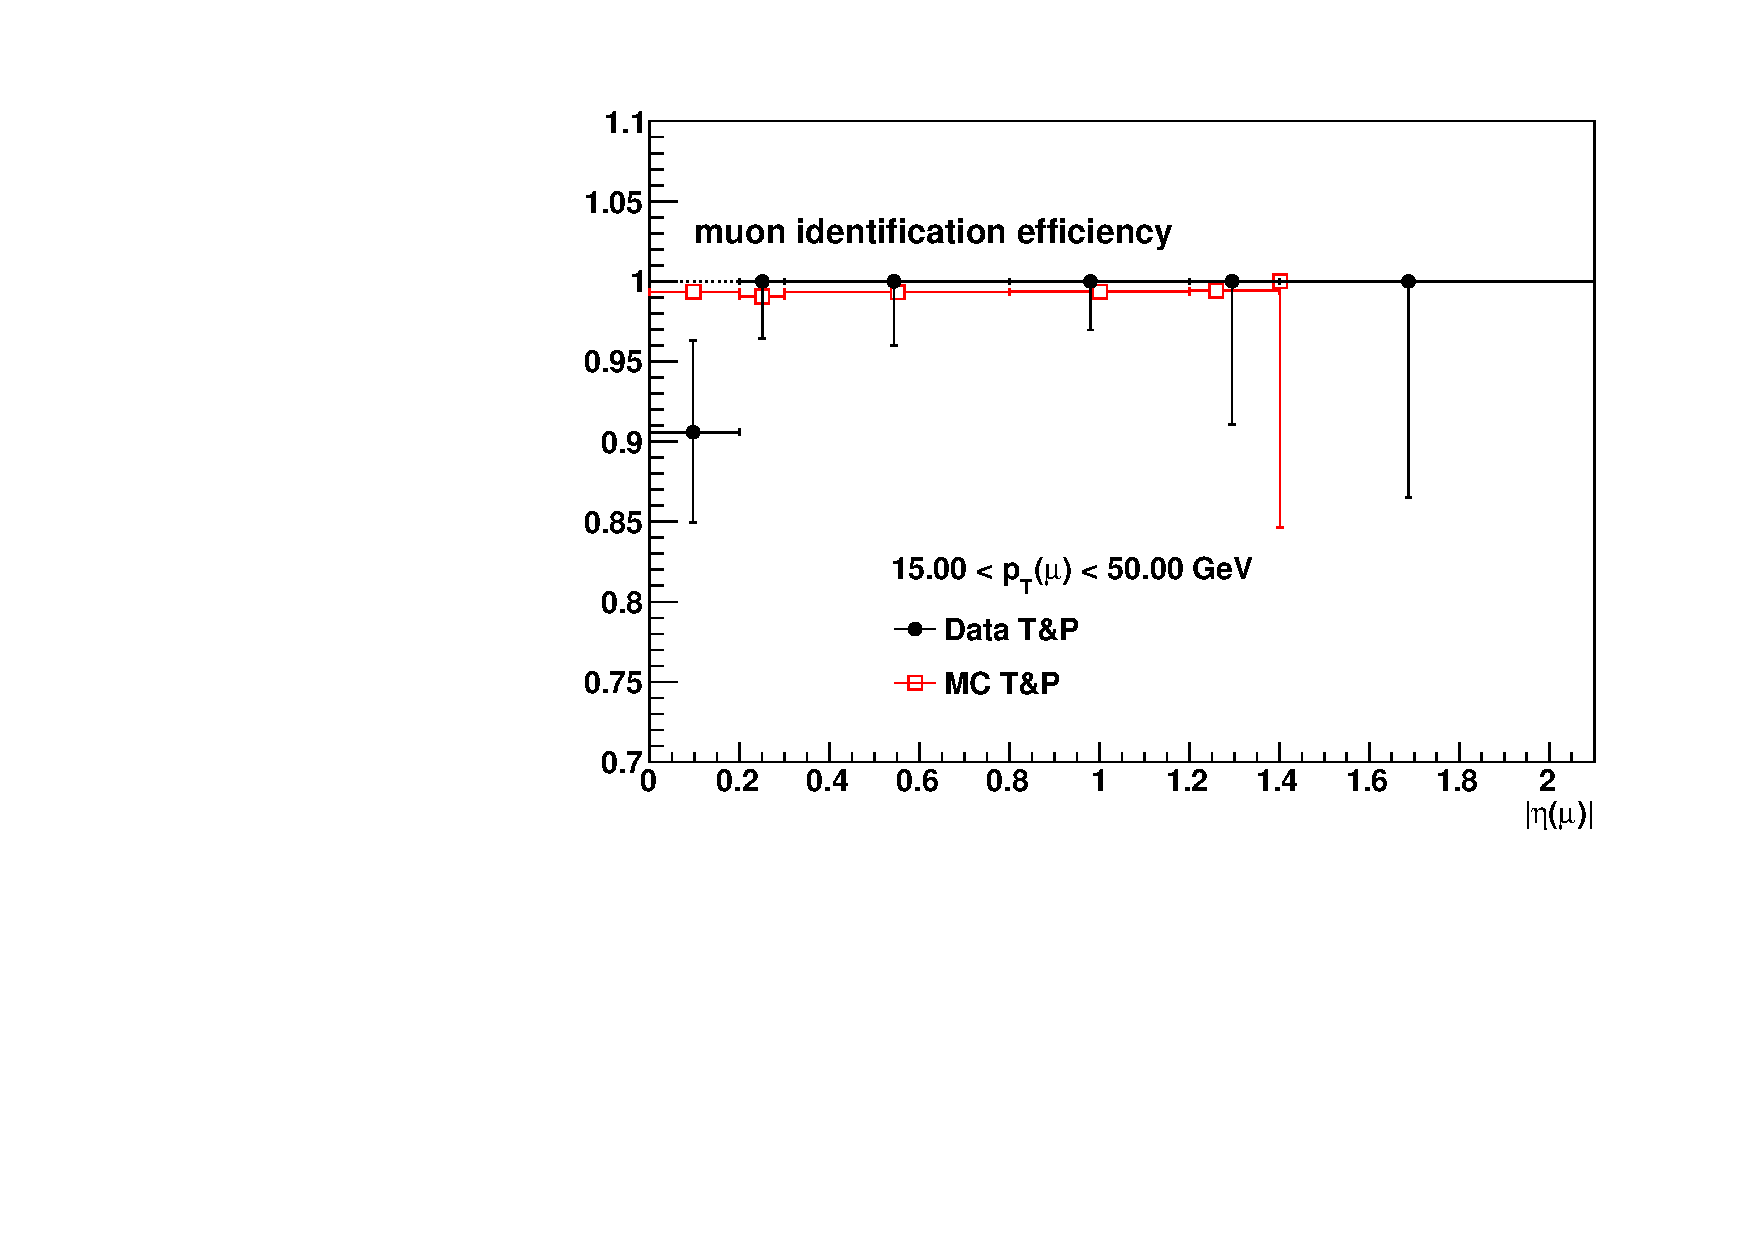
\includegraphics[width=0.49\textwidth]{Figures/\subDirName/MuIDEff_eta_DataVsMC_pTBin7.pdf}
\caption{Muon reconstruction efficiency versus $|\eta|$ for small
  slices in \pt, using the ``tracker50'' muon cuts.}
\label{fig:muonIDEff-eta-1}
\end{figure}
\begin{figure}[p]
\centering
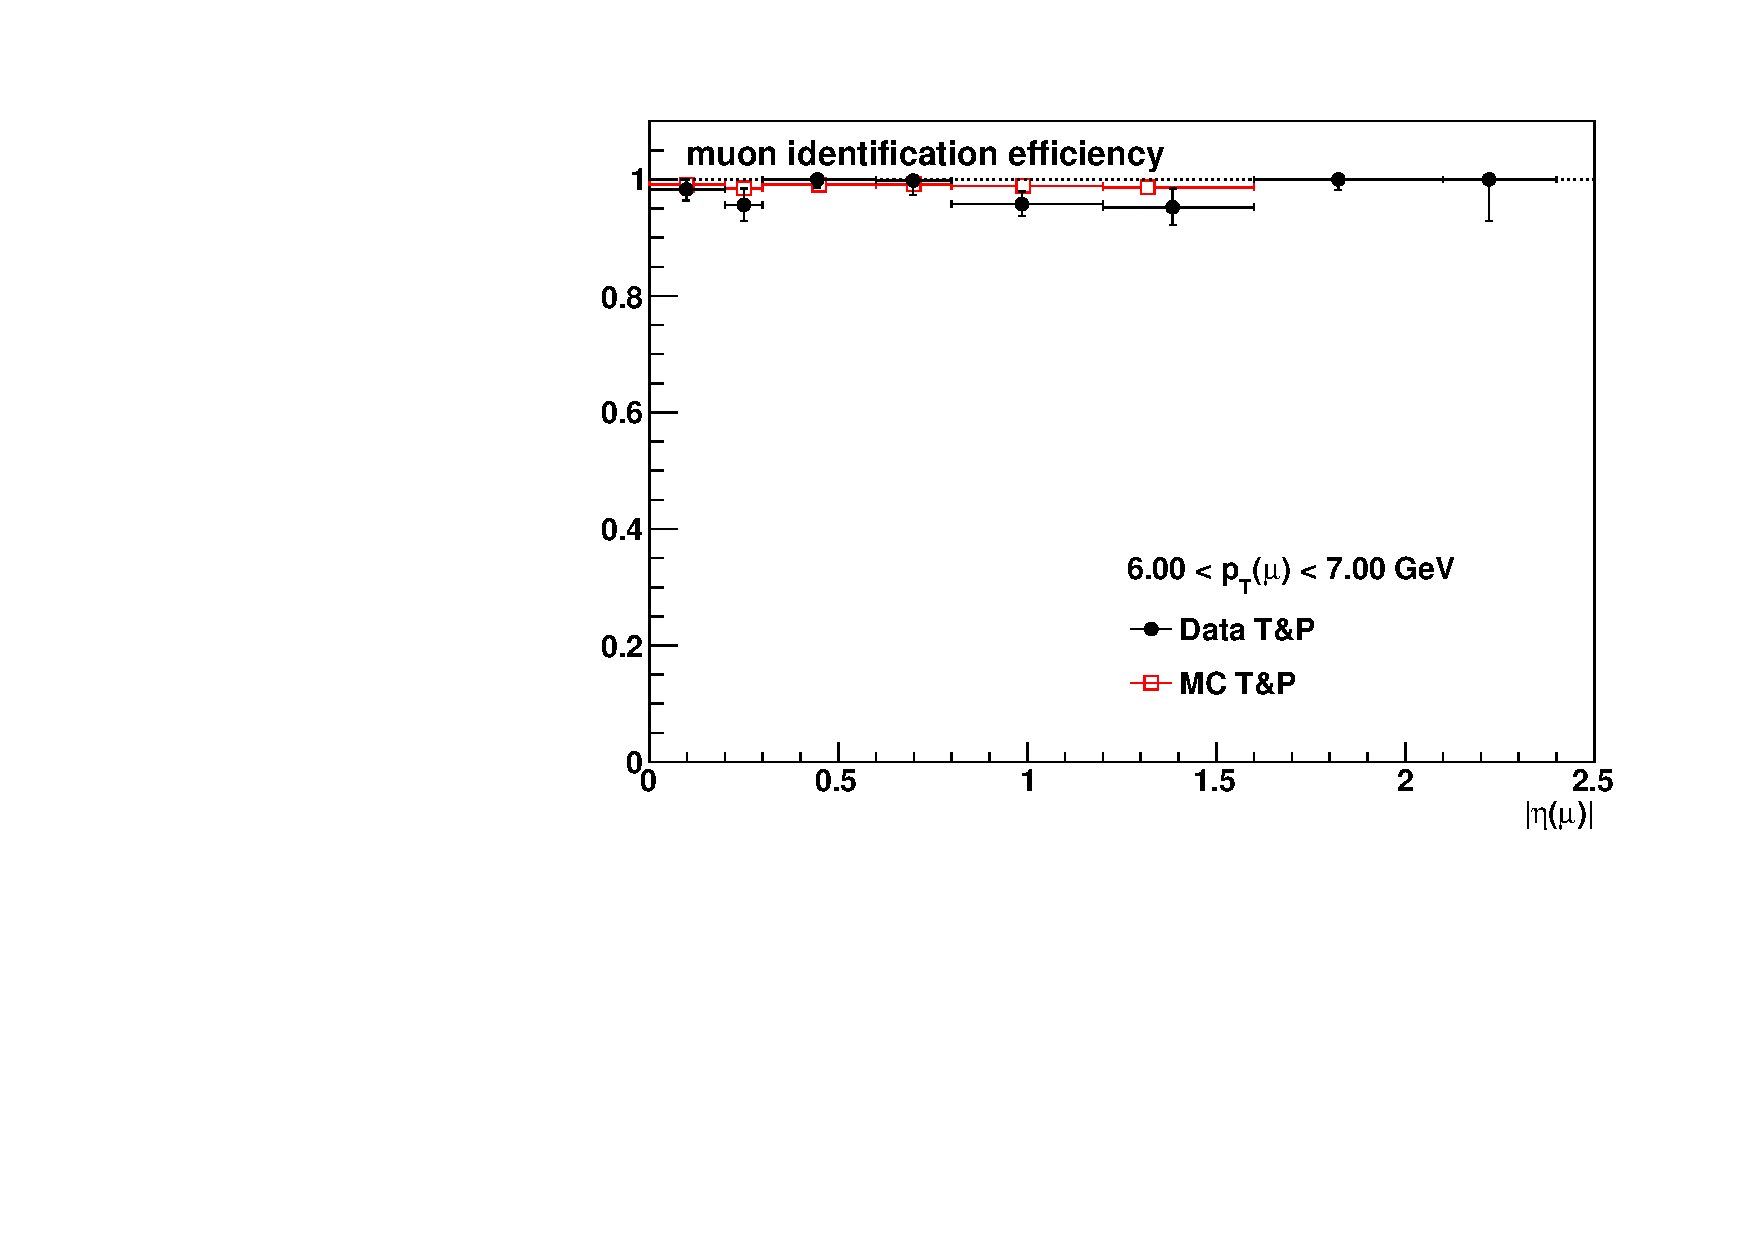
\includegraphics[width=0.49\textwidth]{Figures/\subDirName/MuIDEff_eta_DataVsMC_pTBin8.pdf}
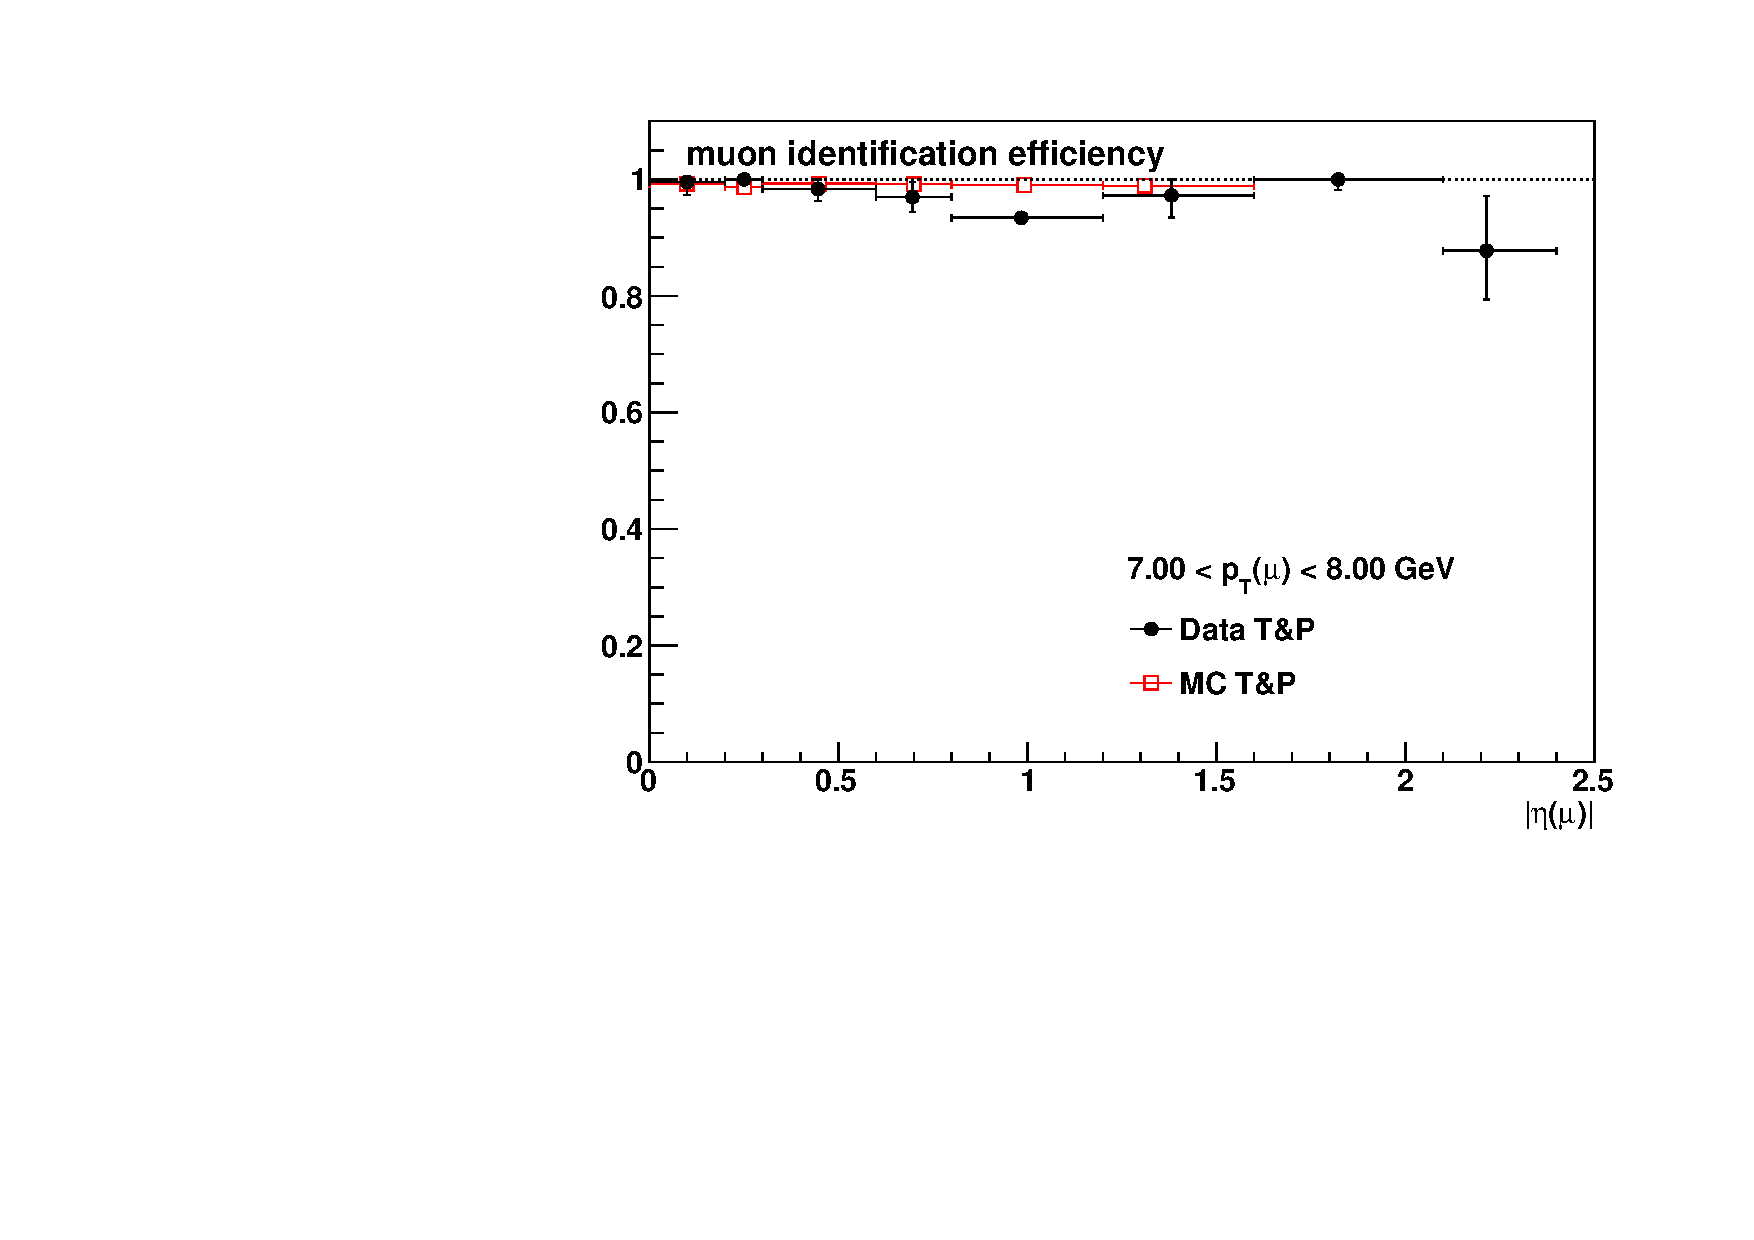
\includegraphics[width=0.49\textwidth]{Figures/\subDirName/MuIDEff_eta_DataVsMC_pTBin9.pdf}
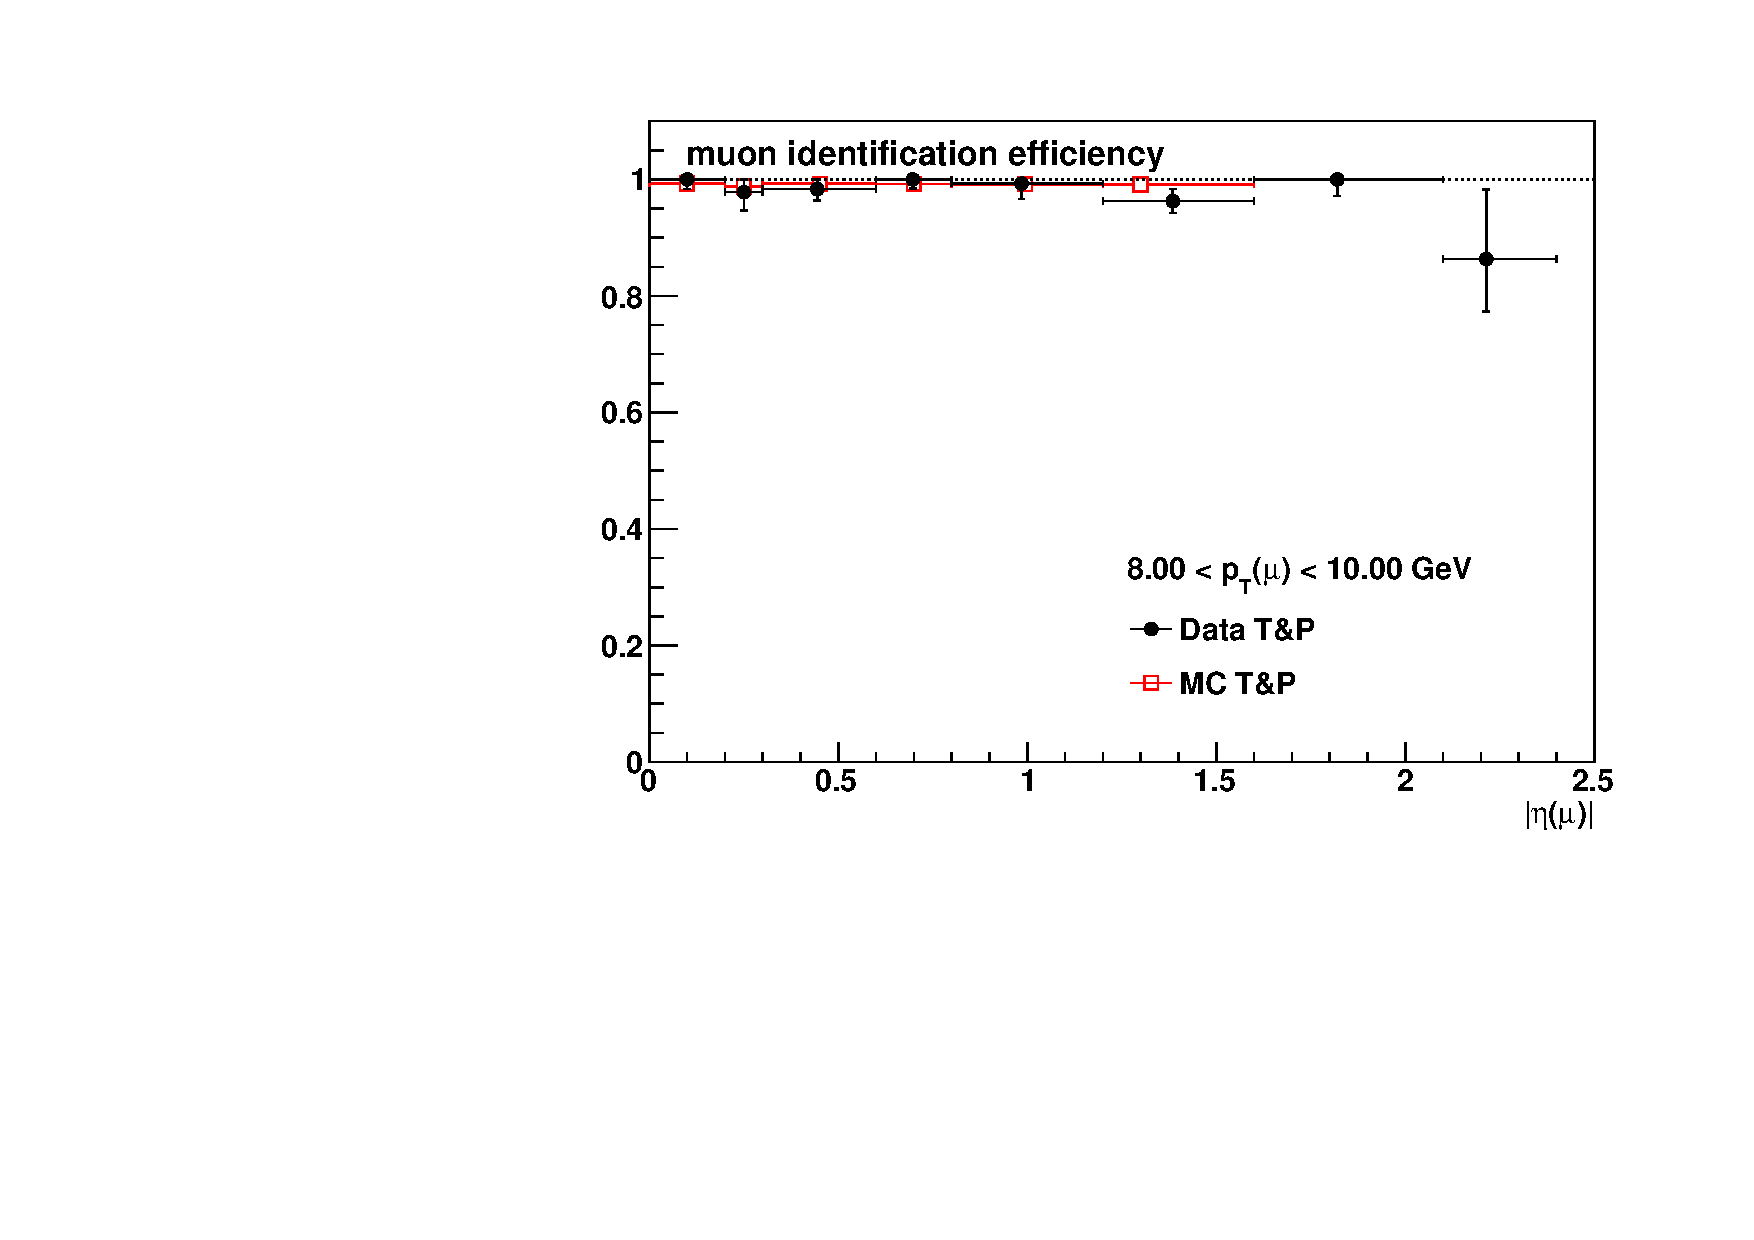
\includegraphics[width=0.49\textwidth]{Figures/\subDirName/MuIDEff_eta_DataVsMC_pTBin10.pdf}
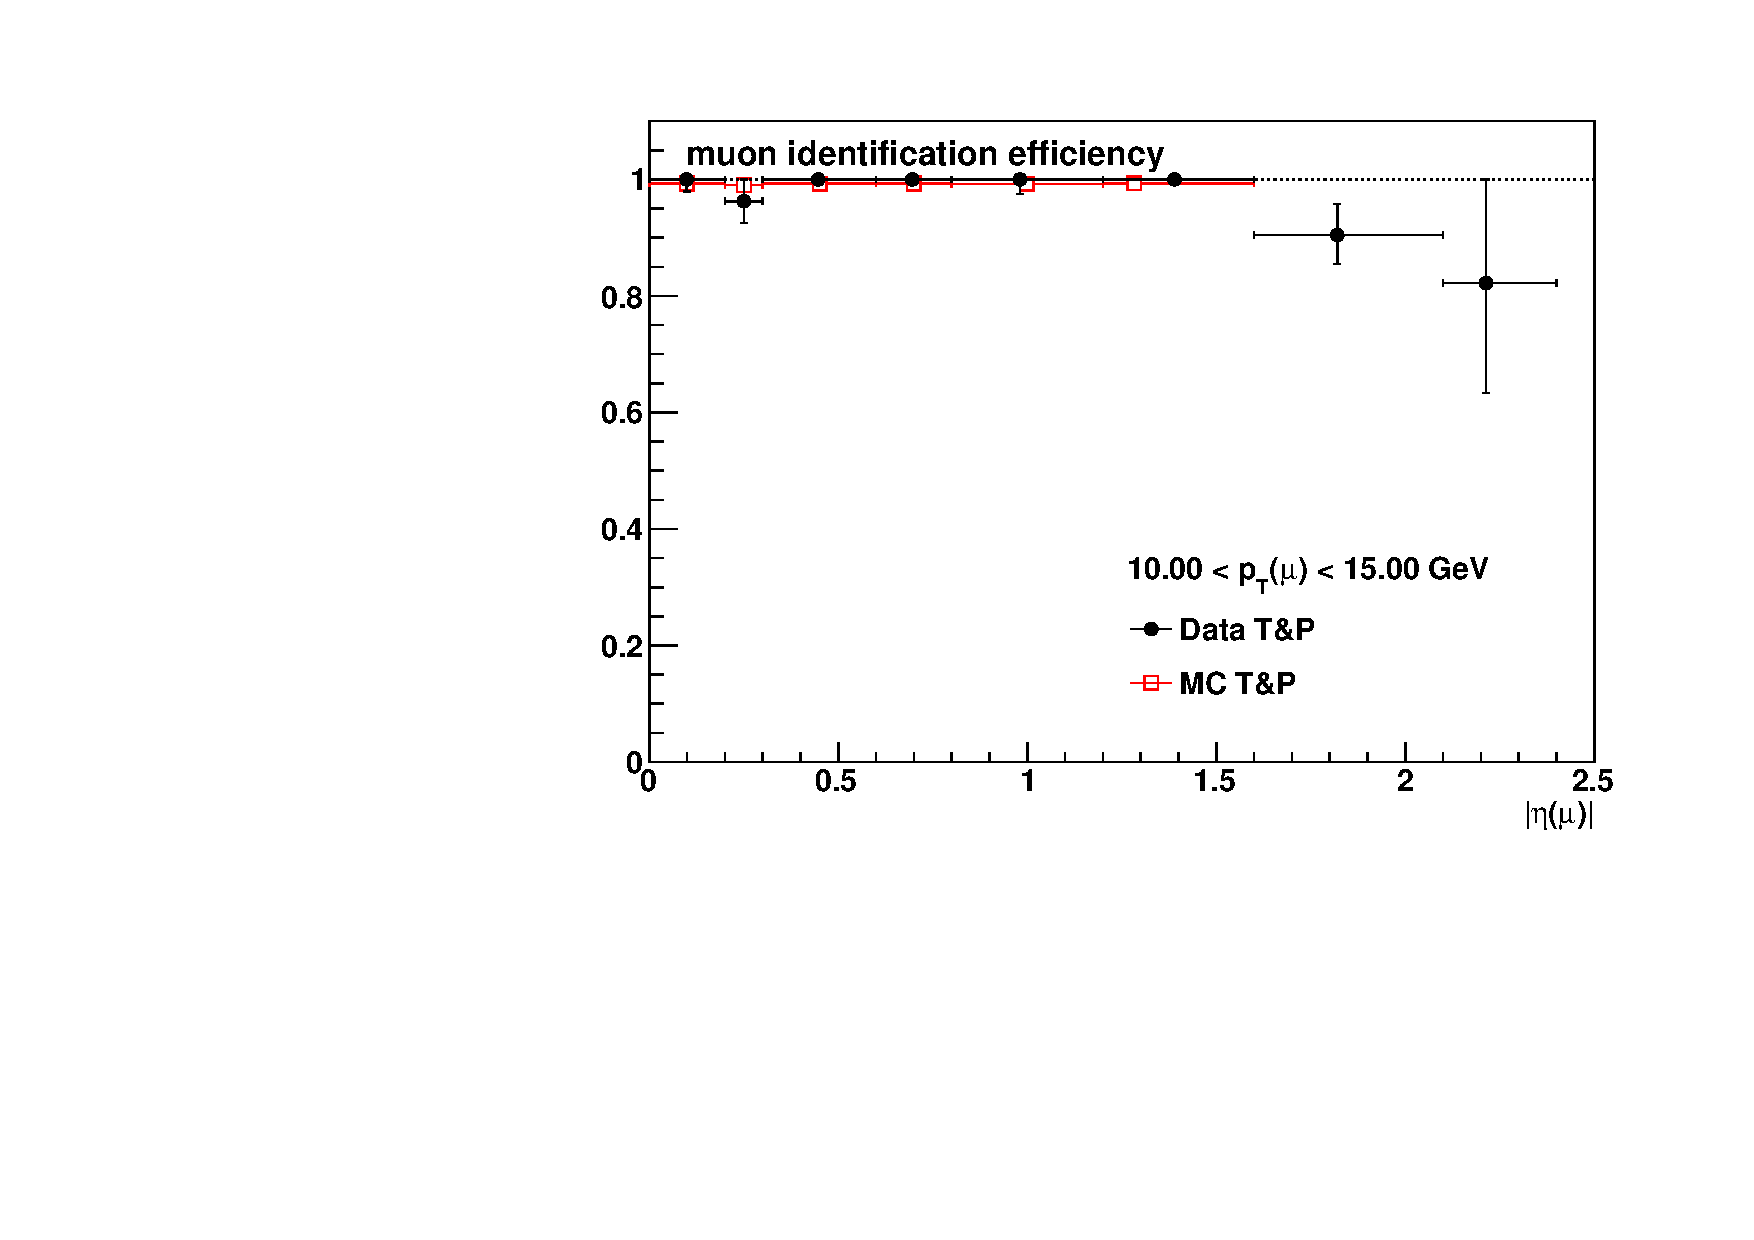
\includegraphics[width=0.49\textwidth]{Figures/\subDirName/MuIDEff_eta_DataVsMC_pTBin11.pdf}
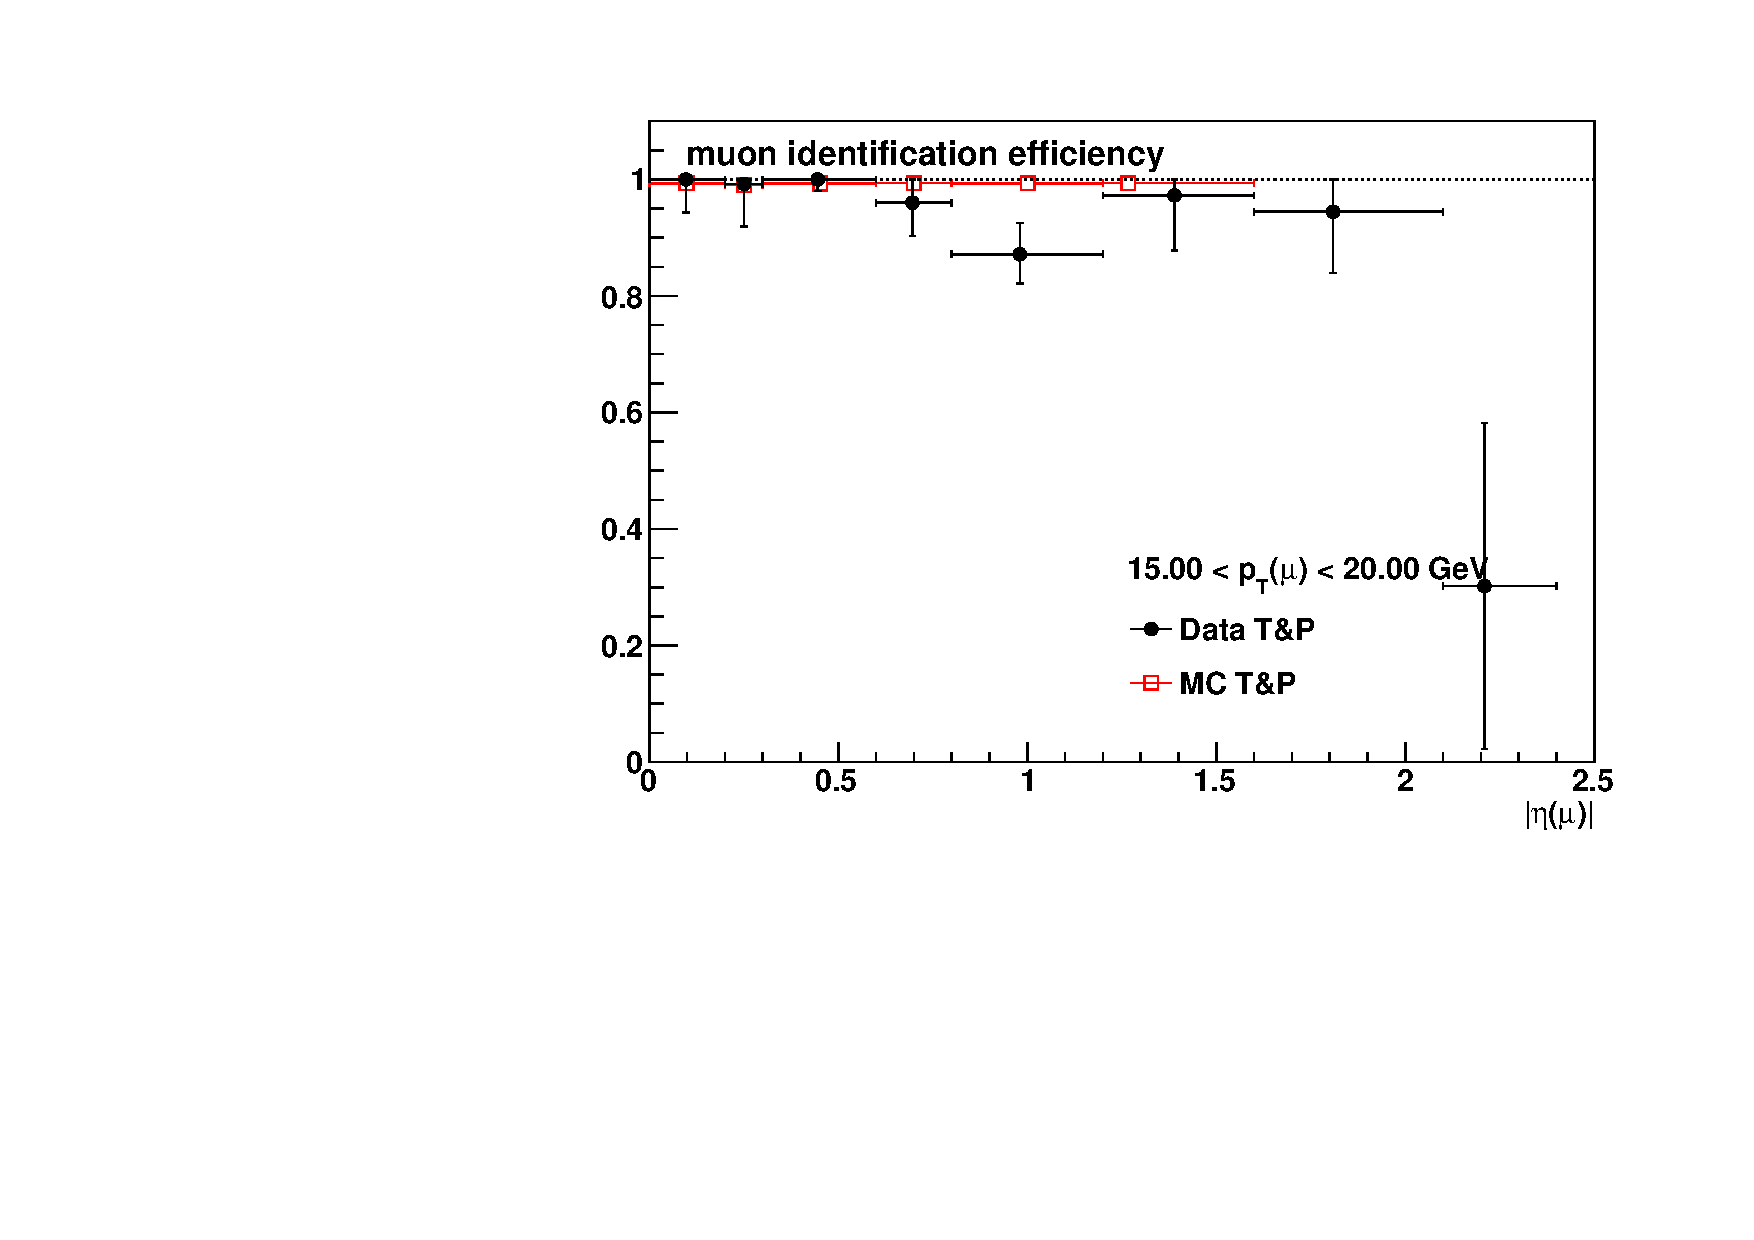
\includegraphics[width=0.49\textwidth]{Figures/\subDirName/MuIDEff_eta_DataVsMC_pTBin12.pdf}
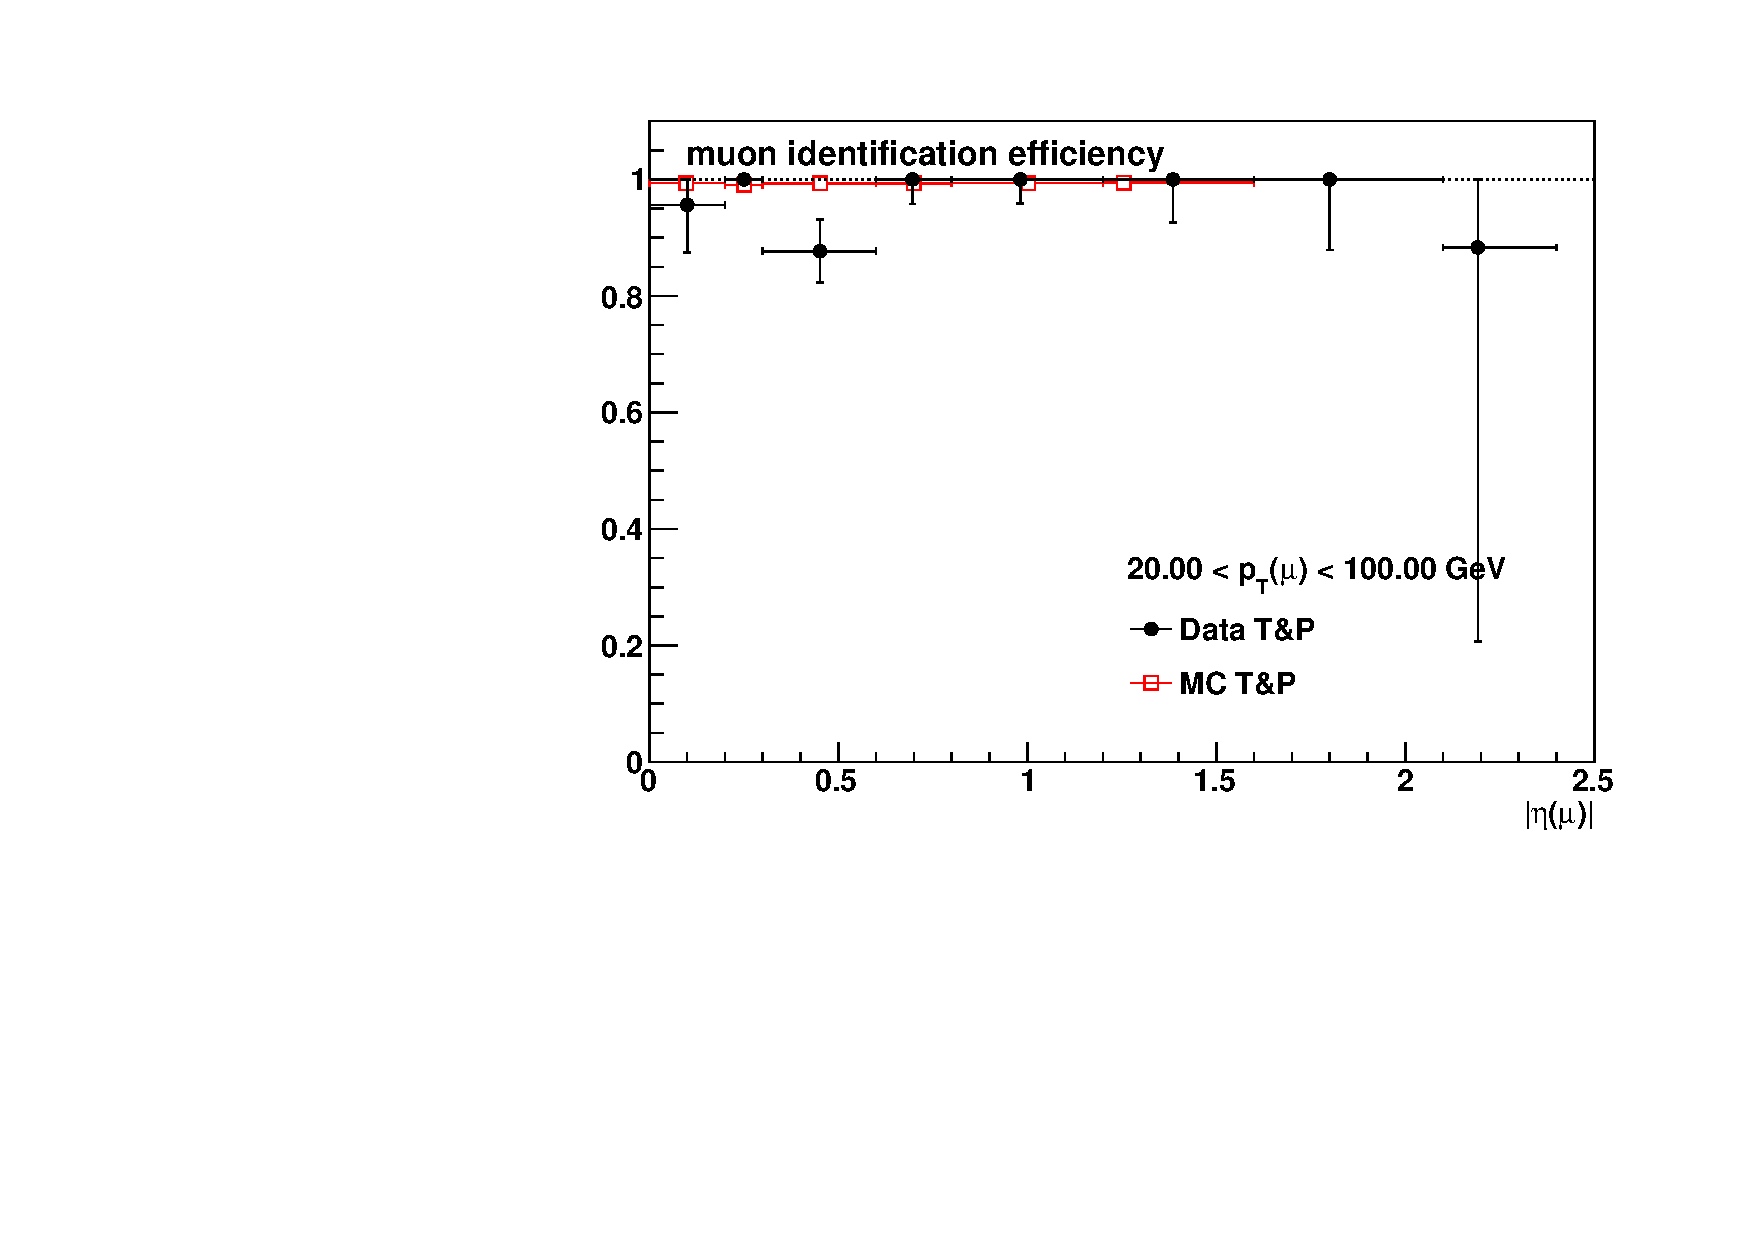
\includegraphics[width=0.49\textwidth]{Figures/\subDirName/MuIDEff_eta_DataVsMC_pTBin13.pdf}
\caption{Continuation of Fig~\ref{fig:muonIDEff-eta-1}.}
\label{fig:muonIDEff-eta-2}
\end{figure}

Given that the probes are all tracks, with no quality requirements
applied, the background in the ``All Probe" and ``Failing Probe"
samples is not negligible, as can be seen in
Fig.~\ref{fig:muonID-abseta4_pt1}. The muon reconstruction
efficiencies are close to 100\,\%. Given the large background and
small signal in the ``Failing probes'' it is difficult to reliably
estimate the efficiency, obtained by the \tnp\ algorithm as a combined
fit to the mass distributions of ``Passing'', ``Failing'' and ``All
Probes''.  The corresponding efficiencies, studied in 2D, are depicted
\pt\ differentially in small slices of $|\eta|$ in
Fig.~\ref{fig:muonIDEff-pt} and $|\eta|$ differentially in small
slices of \pt\ in Fig.~\ref{fig:muonIDEff-eta-1} and \ref{fig:muonIDEff-eta-2}.

Given the difficulties during the fit process, it is understandable
that the trends of the \pt\ differential efficiency curves are not
well established from the \tnp\ studies on real data. The MC consists
of the signal only, and is not affected by this limitation and shows a
rather clear trend, indicating efficiencies larger than 95\,\%,
flattening out at around 8~GeV/$c$. It should be noted that the MC can
describe the data rather accurately, given the large uncertainties. It
could, hence, be favourable in the data analyses to use the MC based
\tnp\ efficiencies instead of the data driven ones. 

The MC based results show somewhat lower efficiencies for the bin $0.2
< |\eta| < 0.3$. This is likely due to the fact that this
pseudo-rapidity interval matches the partly non-instrumented region
between the central and the $\pm 1$ wheels of the muon barrel
detectors, which makes the muon reconstruction exceptionally
inefficient. This is especially true for the low \pt\ bins, where the
``tracker muons'' typically only reach one muon station and are more
easily lost in the gap between the central and $\pm 1$ wheels.


Anticipating the discussion in Section~\ref{sec:cowboy}, we want to
underline that we studied the muon reconstruction efficiency
separately for ``cowboy'' and ``seagull'' dimuons, boh in data as well
as MC, and do not find any differences. This is due to the fact that
we only consider tracker muons (or global muons which also qualify as
arbitrated tracker muons) which are subject to different
reconstruction algorithms, not being affected by the inefficiencies
seen for L1, L2 and standalone muons in CMS. For this reason, the muon
reconstruction efficiency, as well as the efficiency of the muon
quality cuts were studied on the basis of all pairs.

%%%%%%%%%%%%%%%%%%%%%%%%%%%%%%%%%%%%%%
\section{Efficiencies of the muon tracking quality cuts}\label{sec:muQual}

The probes for the efficiency study of the muon tracking quality cuts
are the passing probes of the previous step, the ``BMuons", and are
matched to the \texttt{L2Mu2} leg of the efficiency trigger
path. Passing probes are those that satisfy the series of
tracking related quality cuts (``BMuQual"):
\begin{itemize}
\item \texttt{numberOfValidHits} $>10$
\item $\chi^2$ / ndf $<1.8$
\item \texttt{TMOneStationTight}
\item \texttt{pixelLayersWithMeasurement} $>1$
\item $|dB| < 3.0$~cm and $|dz|  < 30$~cm.
\end{itemize}

These are cuts widely used in the quarkonium related
analyses. According to the efficiency studies shown in
Fig.~\ref{fig:muQualEff-pt}, Fig.~\ref{fig:muQualEff-eta-1} and
\ref{fig:muQualEff-eta-2} the efficiencies of these cuts are slightly
$|\eta|$ dependent, with only a mild \pt\ turn-on behaviour, being
between 96\,\% and 98\,\% for $p_{\rm T} > 10$~GeV/$c$. The background
under the \jpsi\ peak in the three probe samples (``Passing'',
``Failing'' and ``All'' probes) is rather small and the analysed
sample is also large enough such that the data driven efficiencies are
obtained with a good statistical accuracy, showing a clear trend,
faithfully reproduced by the MC \tnp\ efficiencies.
%, except for the
%most forward bin, $1.4 < |\eta| < 2.1$. The data seem to show an
%efficiency higher by $\sim 1-2$\,\%.

\begin{figure}[p]
\centering
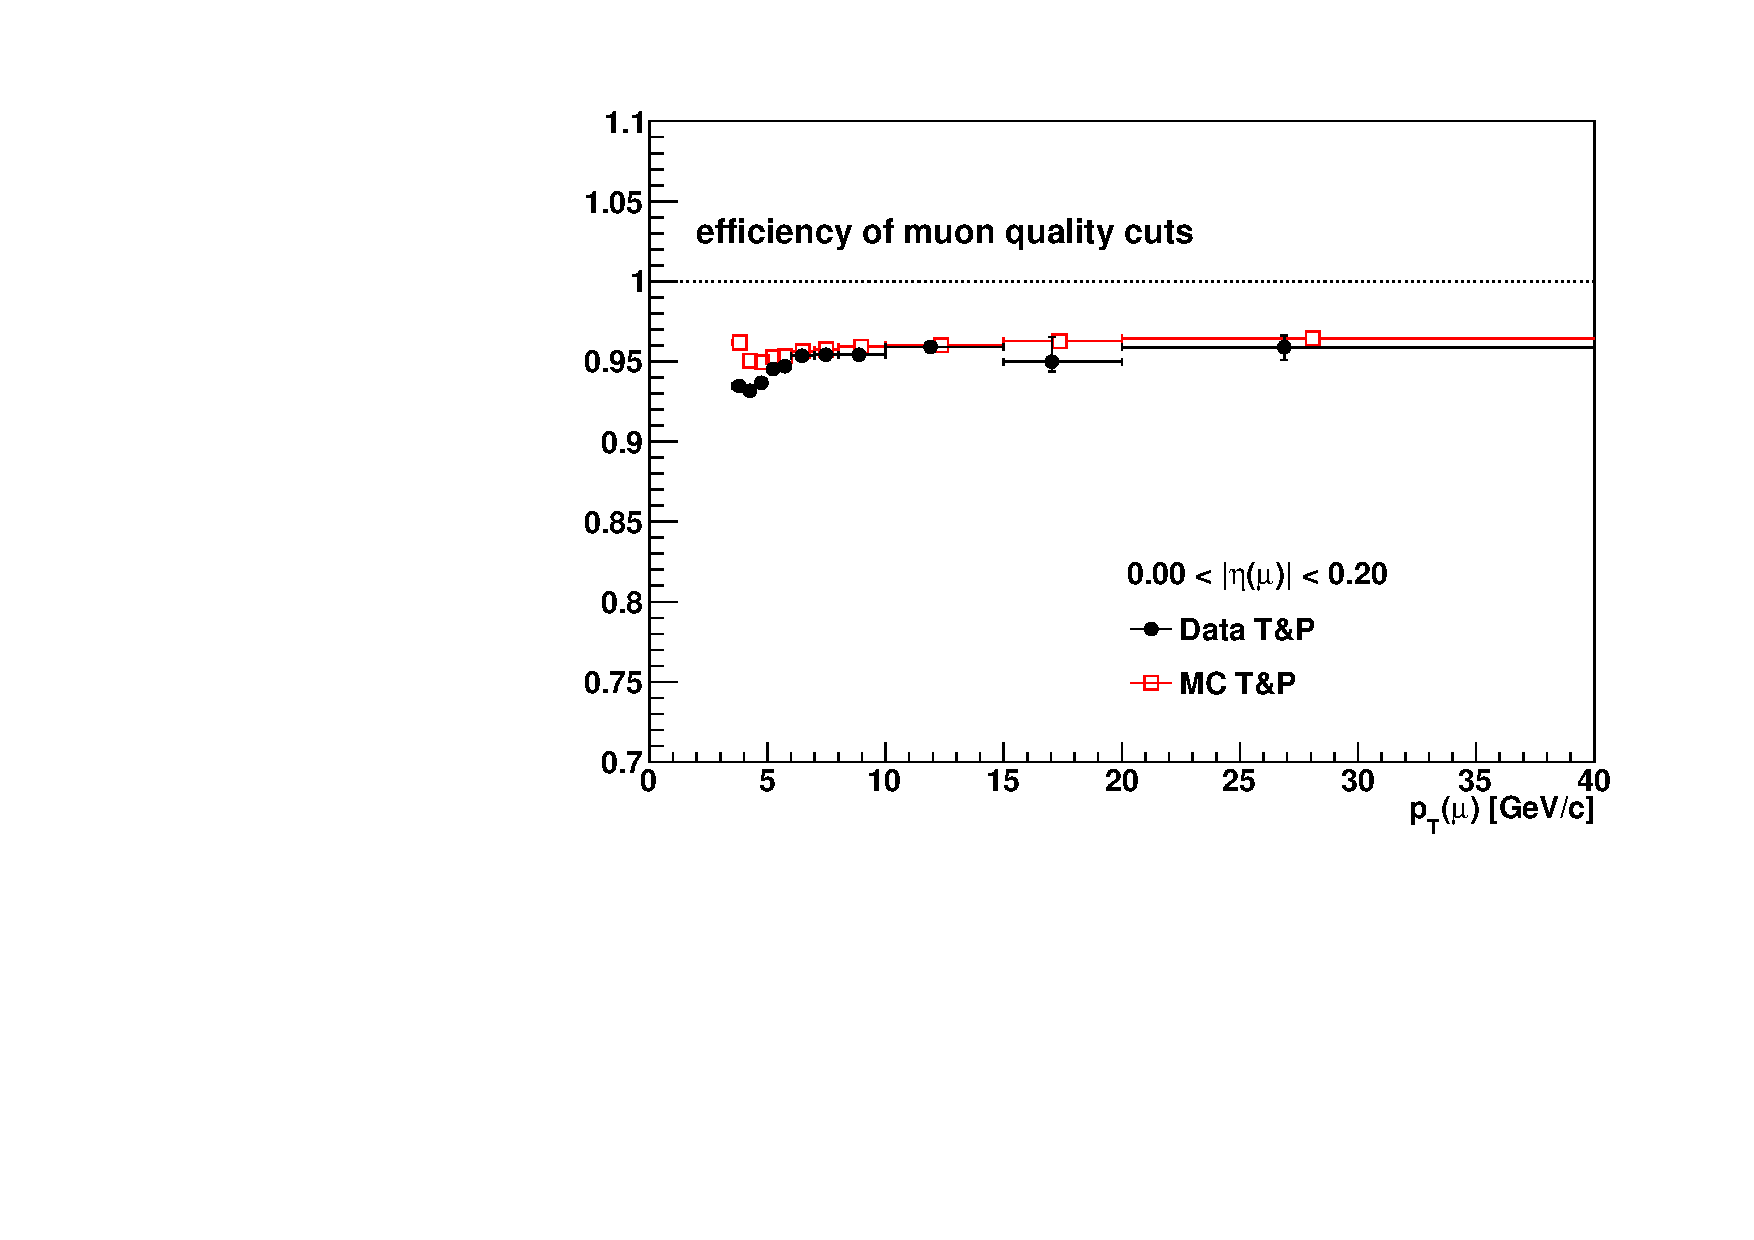
\includegraphics[width=0.49\textwidth]{Figures/\subDirName/MuQualEff_pT_DataVsMC_etaBin0.pdf}
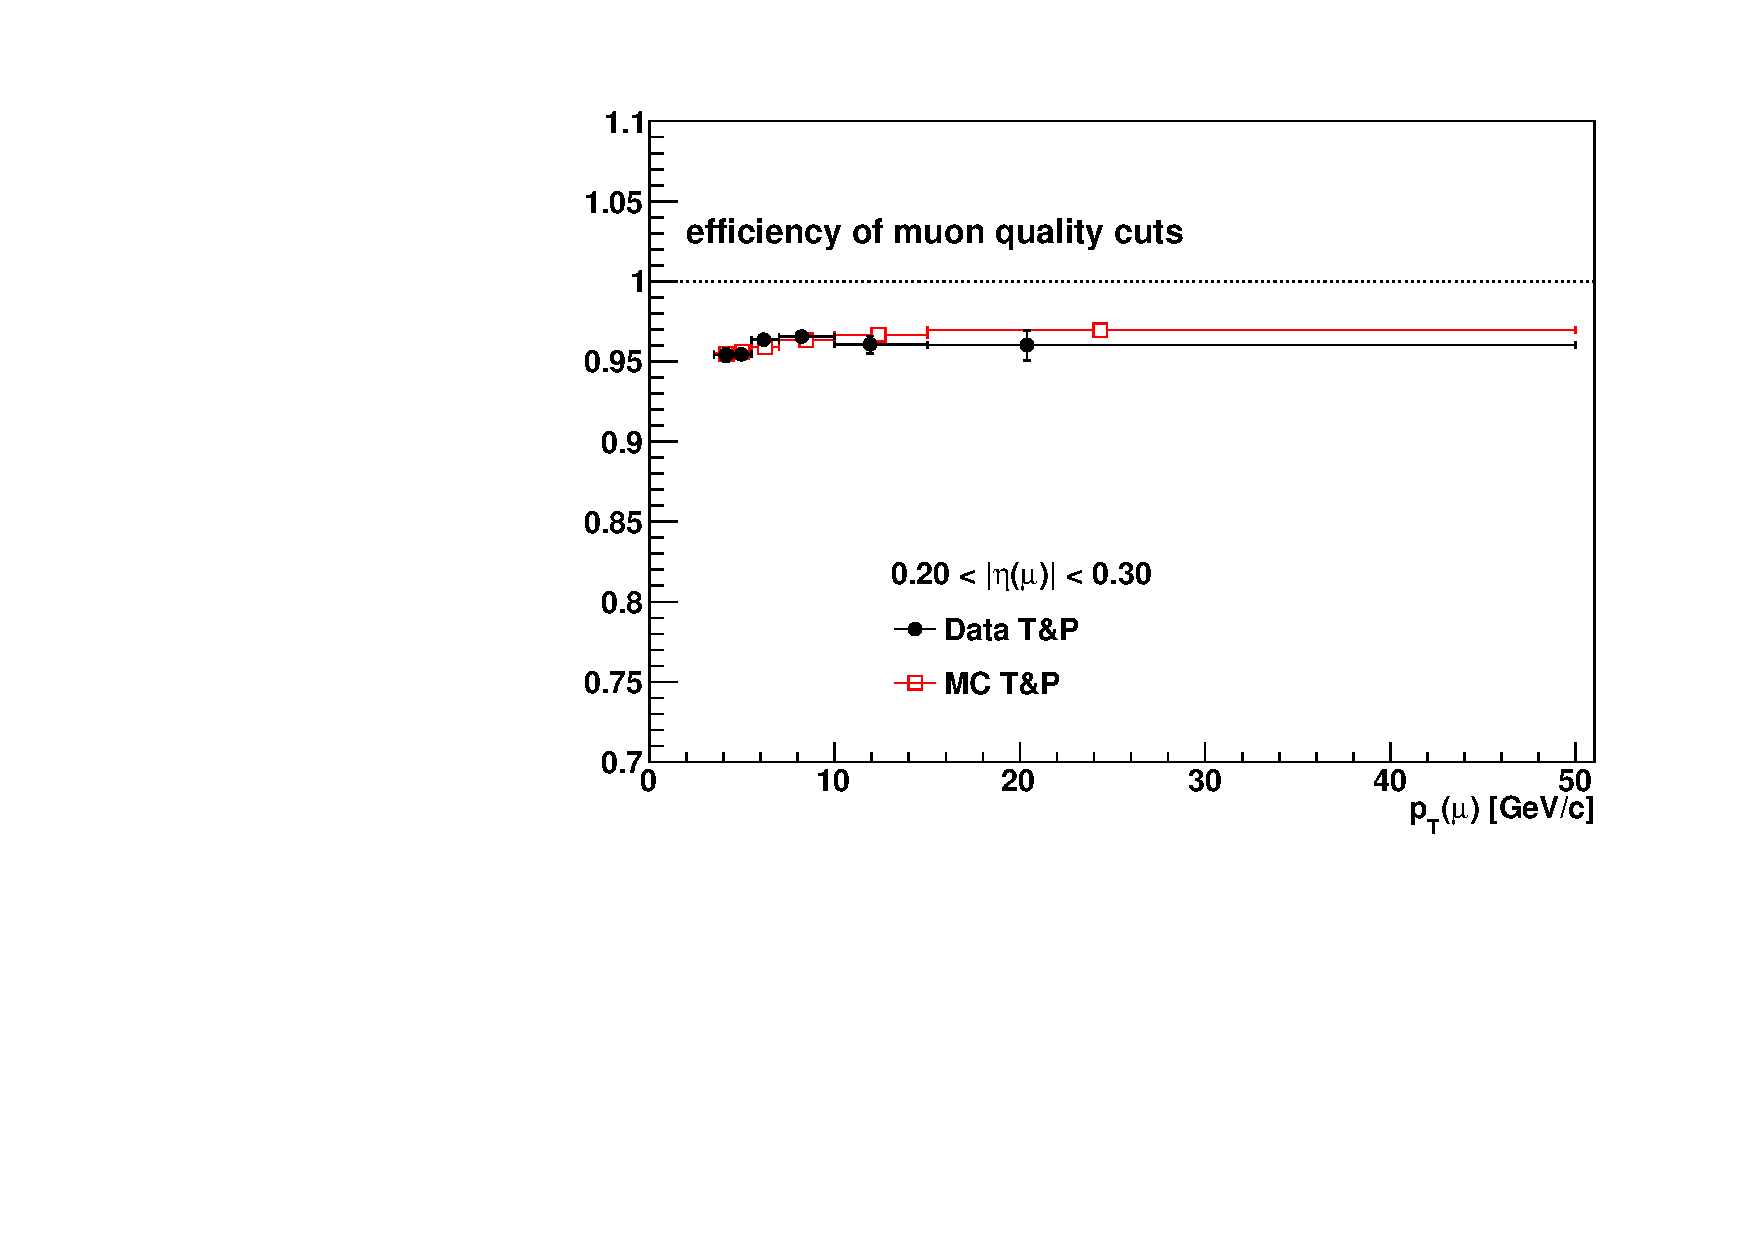
\includegraphics[width=0.49\textwidth]{Figures/\subDirName/MuQualEff_pT_DataVsMC_etaBin1.pdf}
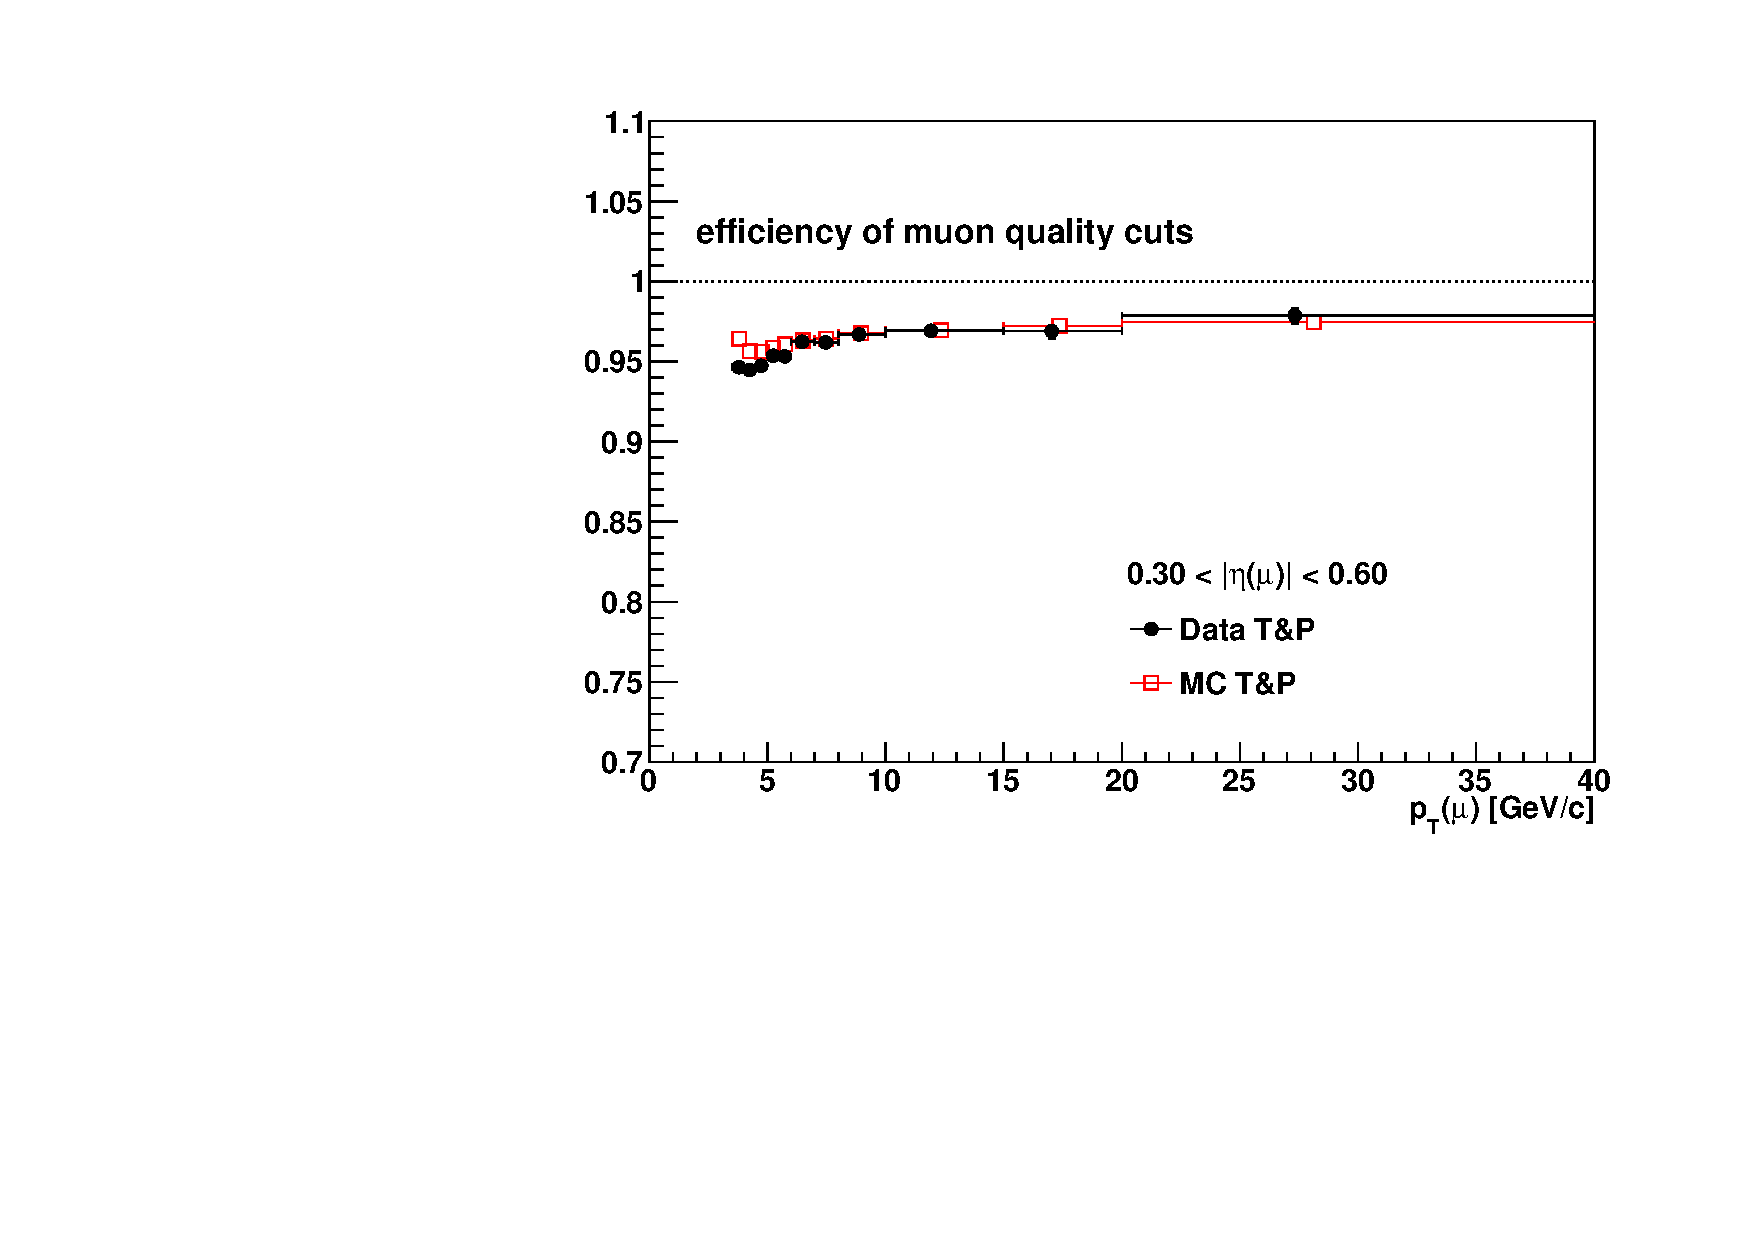
\includegraphics[width=0.49\textwidth]{Figures/\subDirName/MuQualEff_pT_DataVsMC_etaBin2.pdf}
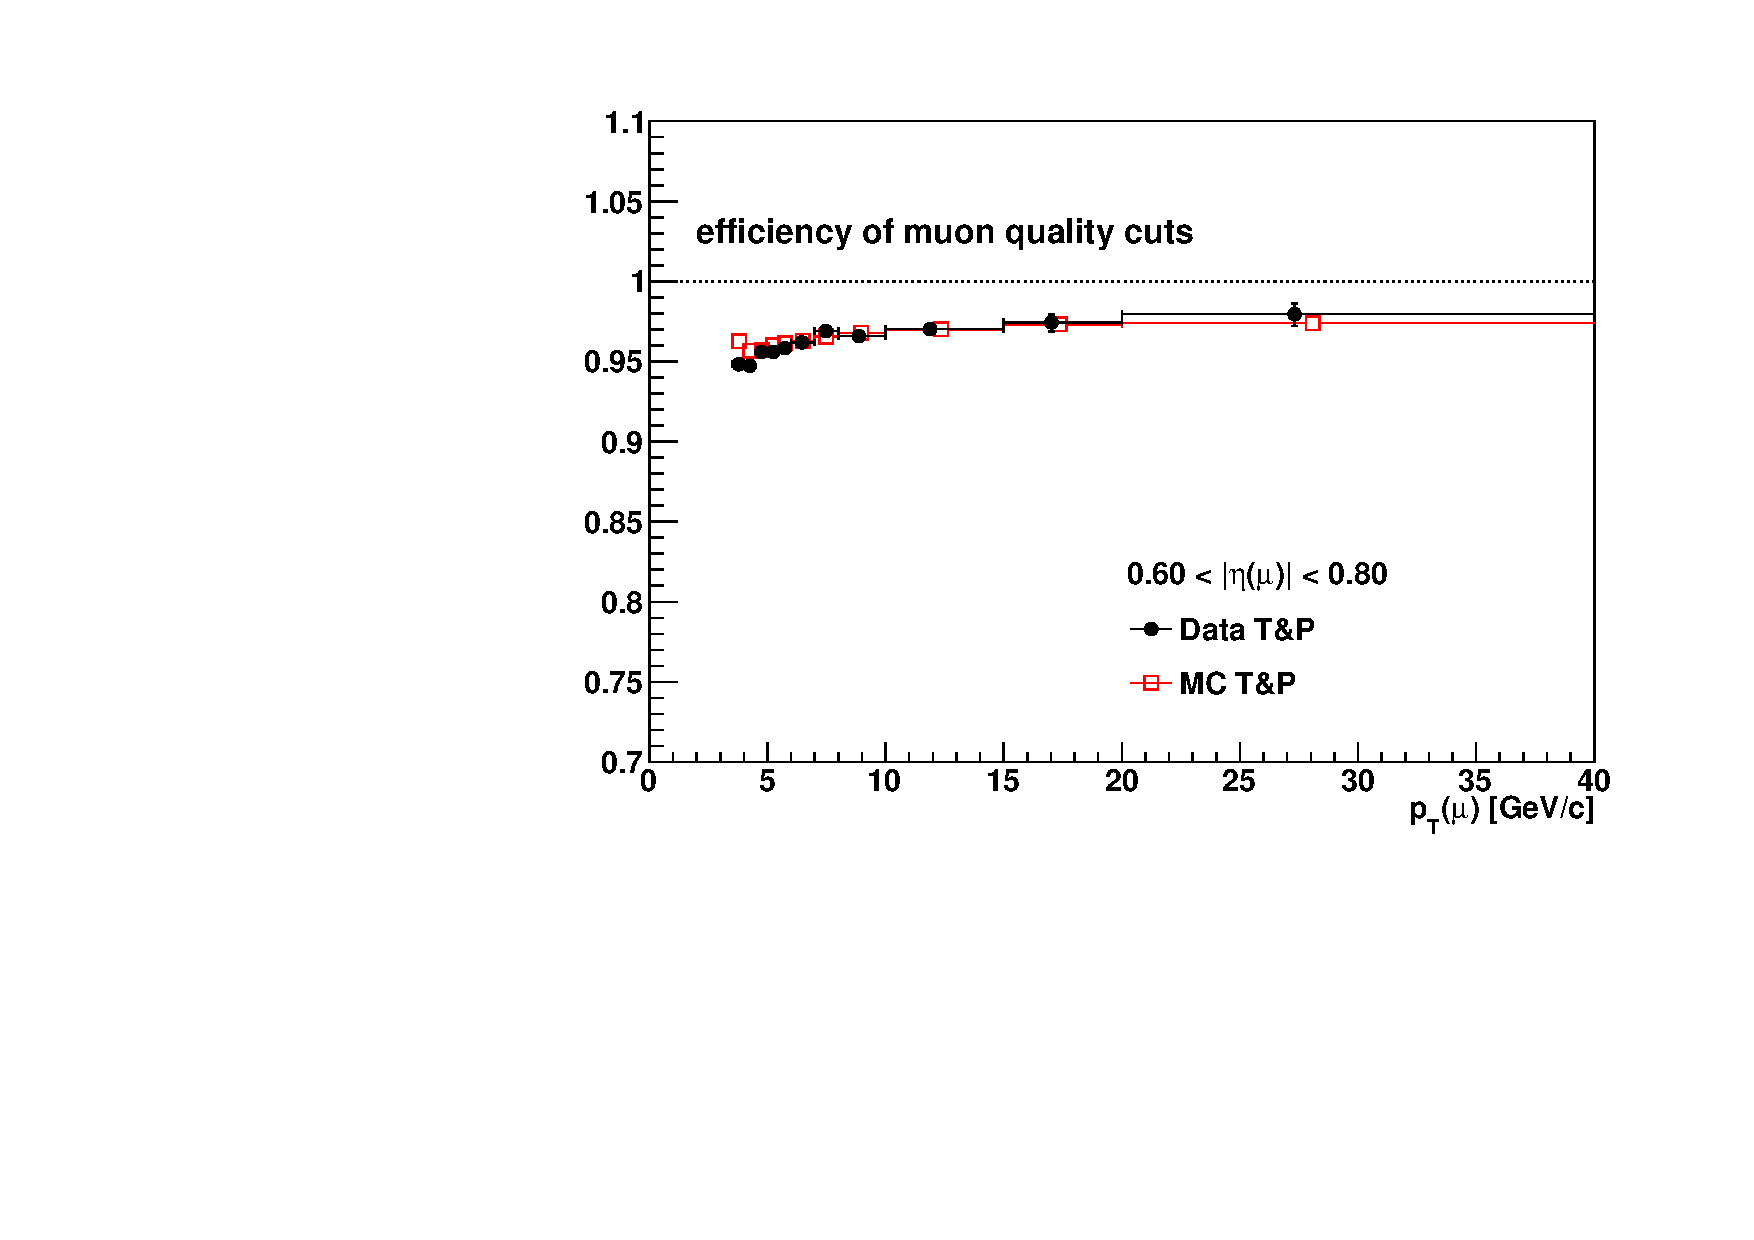
\includegraphics[width=0.49\textwidth]{Figures/\subDirName/MuQualEff_pT_DataVsMC_etaBin3.pdf}
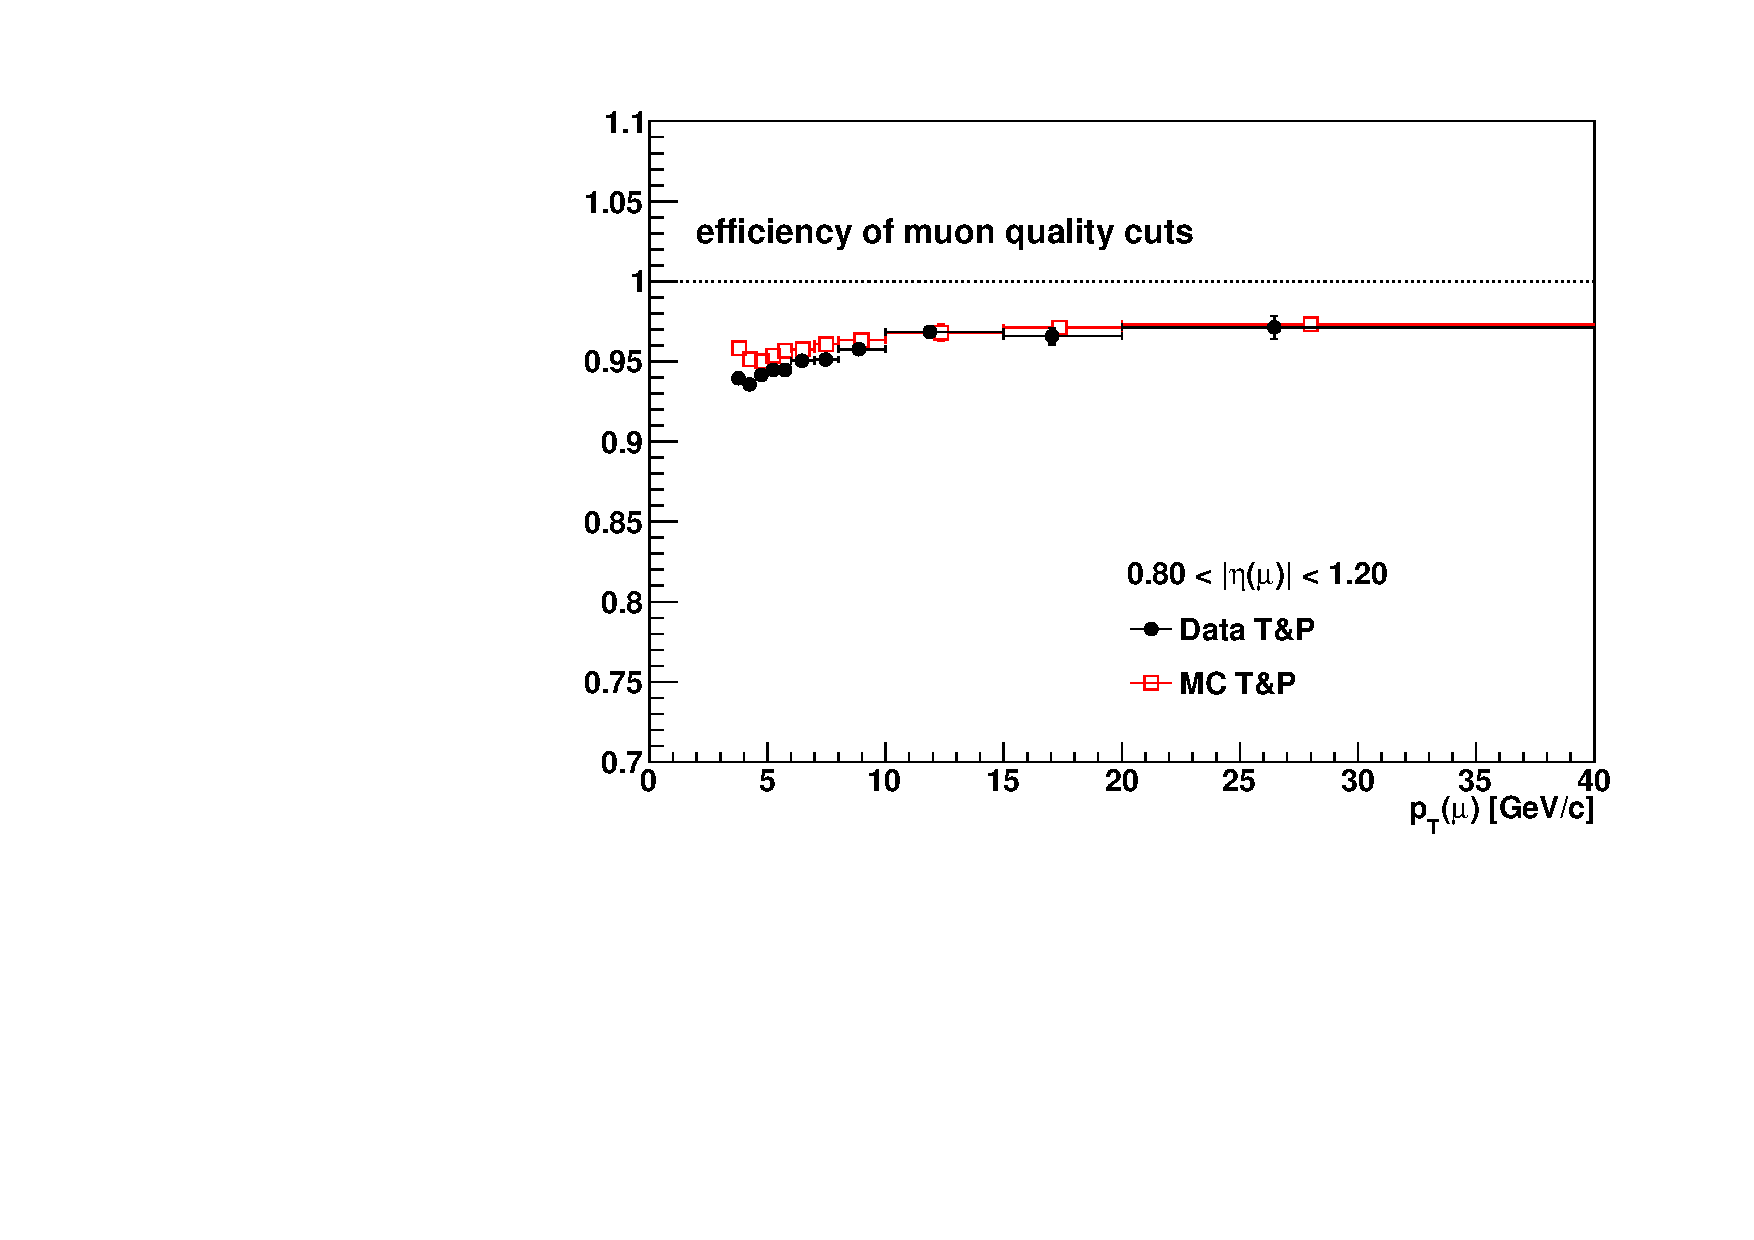
\includegraphics[width=0.49\textwidth]{Figures/\subDirName/MuQualEff_pT_DataVsMC_etaBin4.pdf}
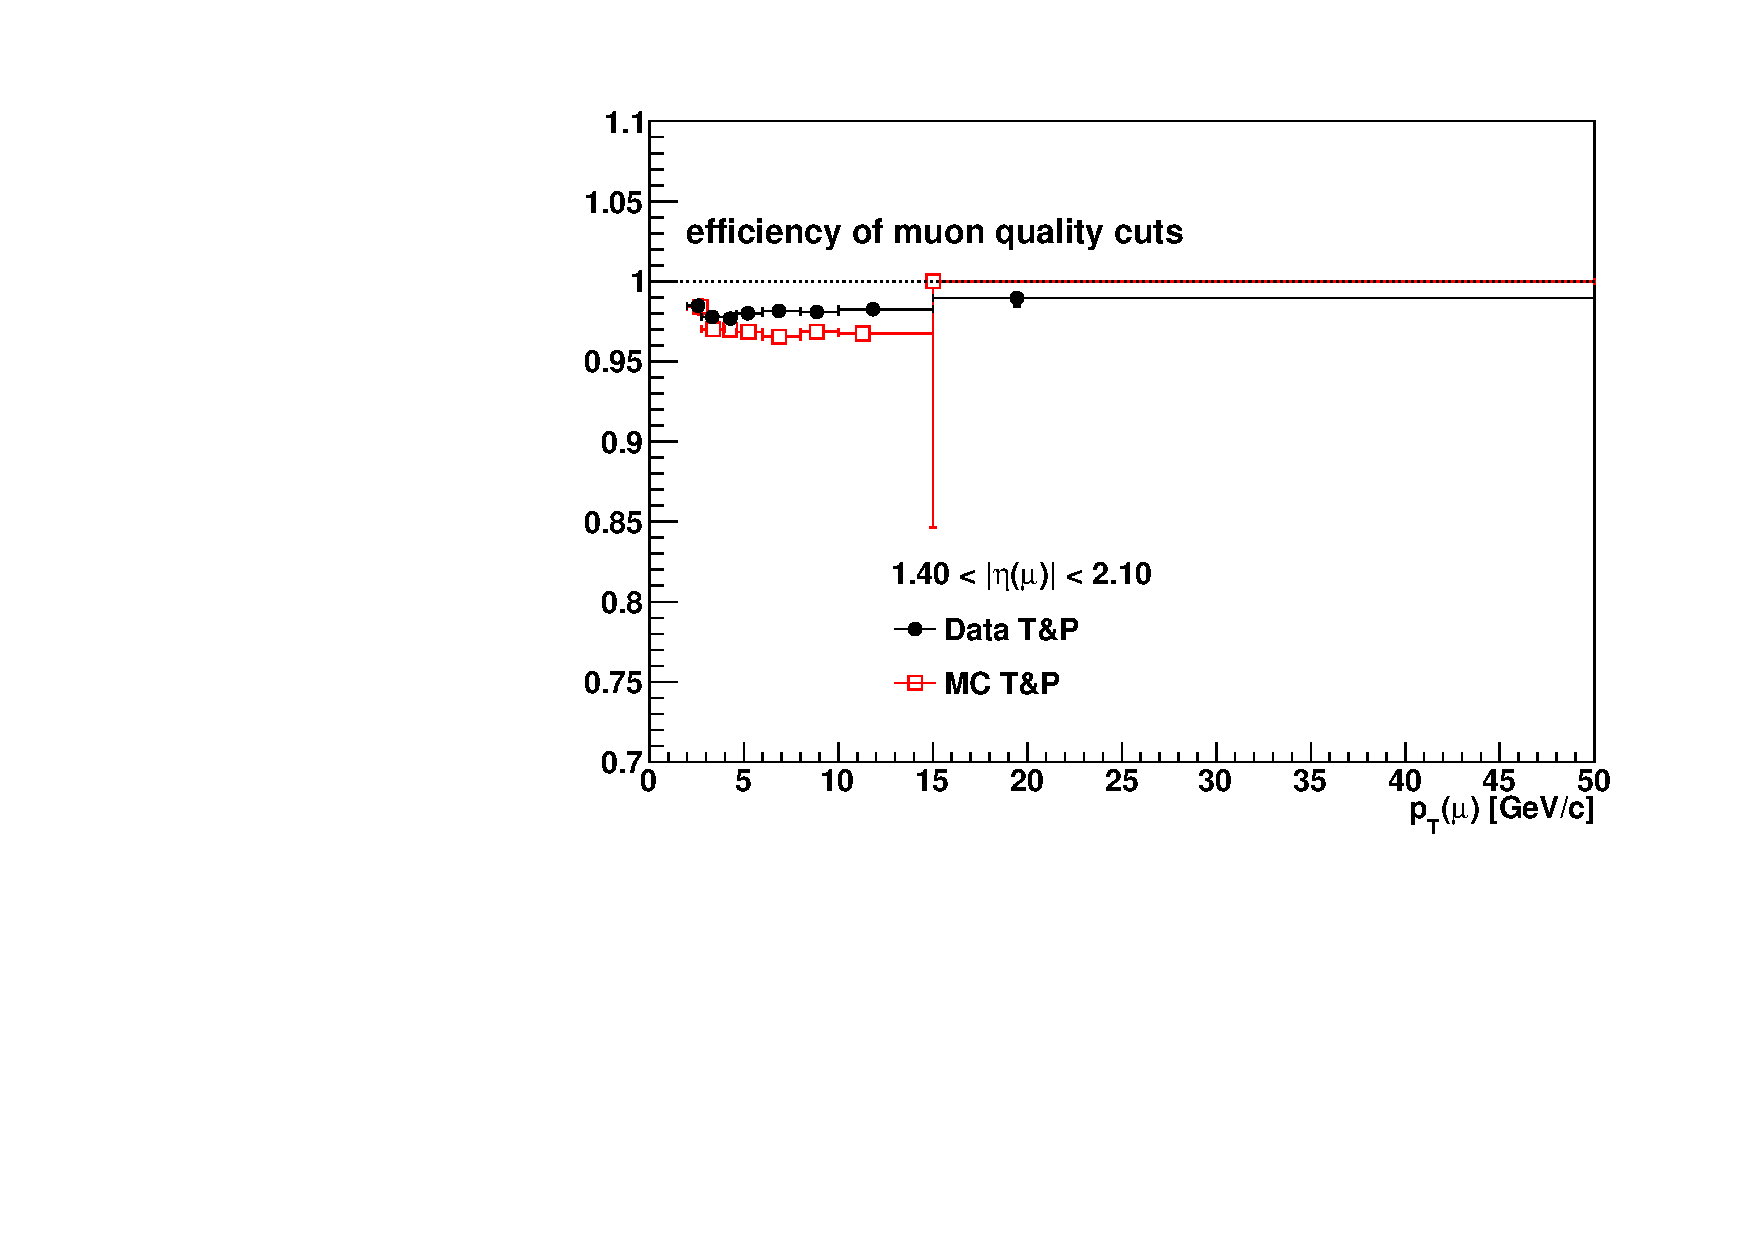
\includegraphics[width=0.49\textwidth]{Figures/\subDirName/MuQualEff_pT_DataVsMC_etaBin5.pdf}
%only for Tracker muon cuts
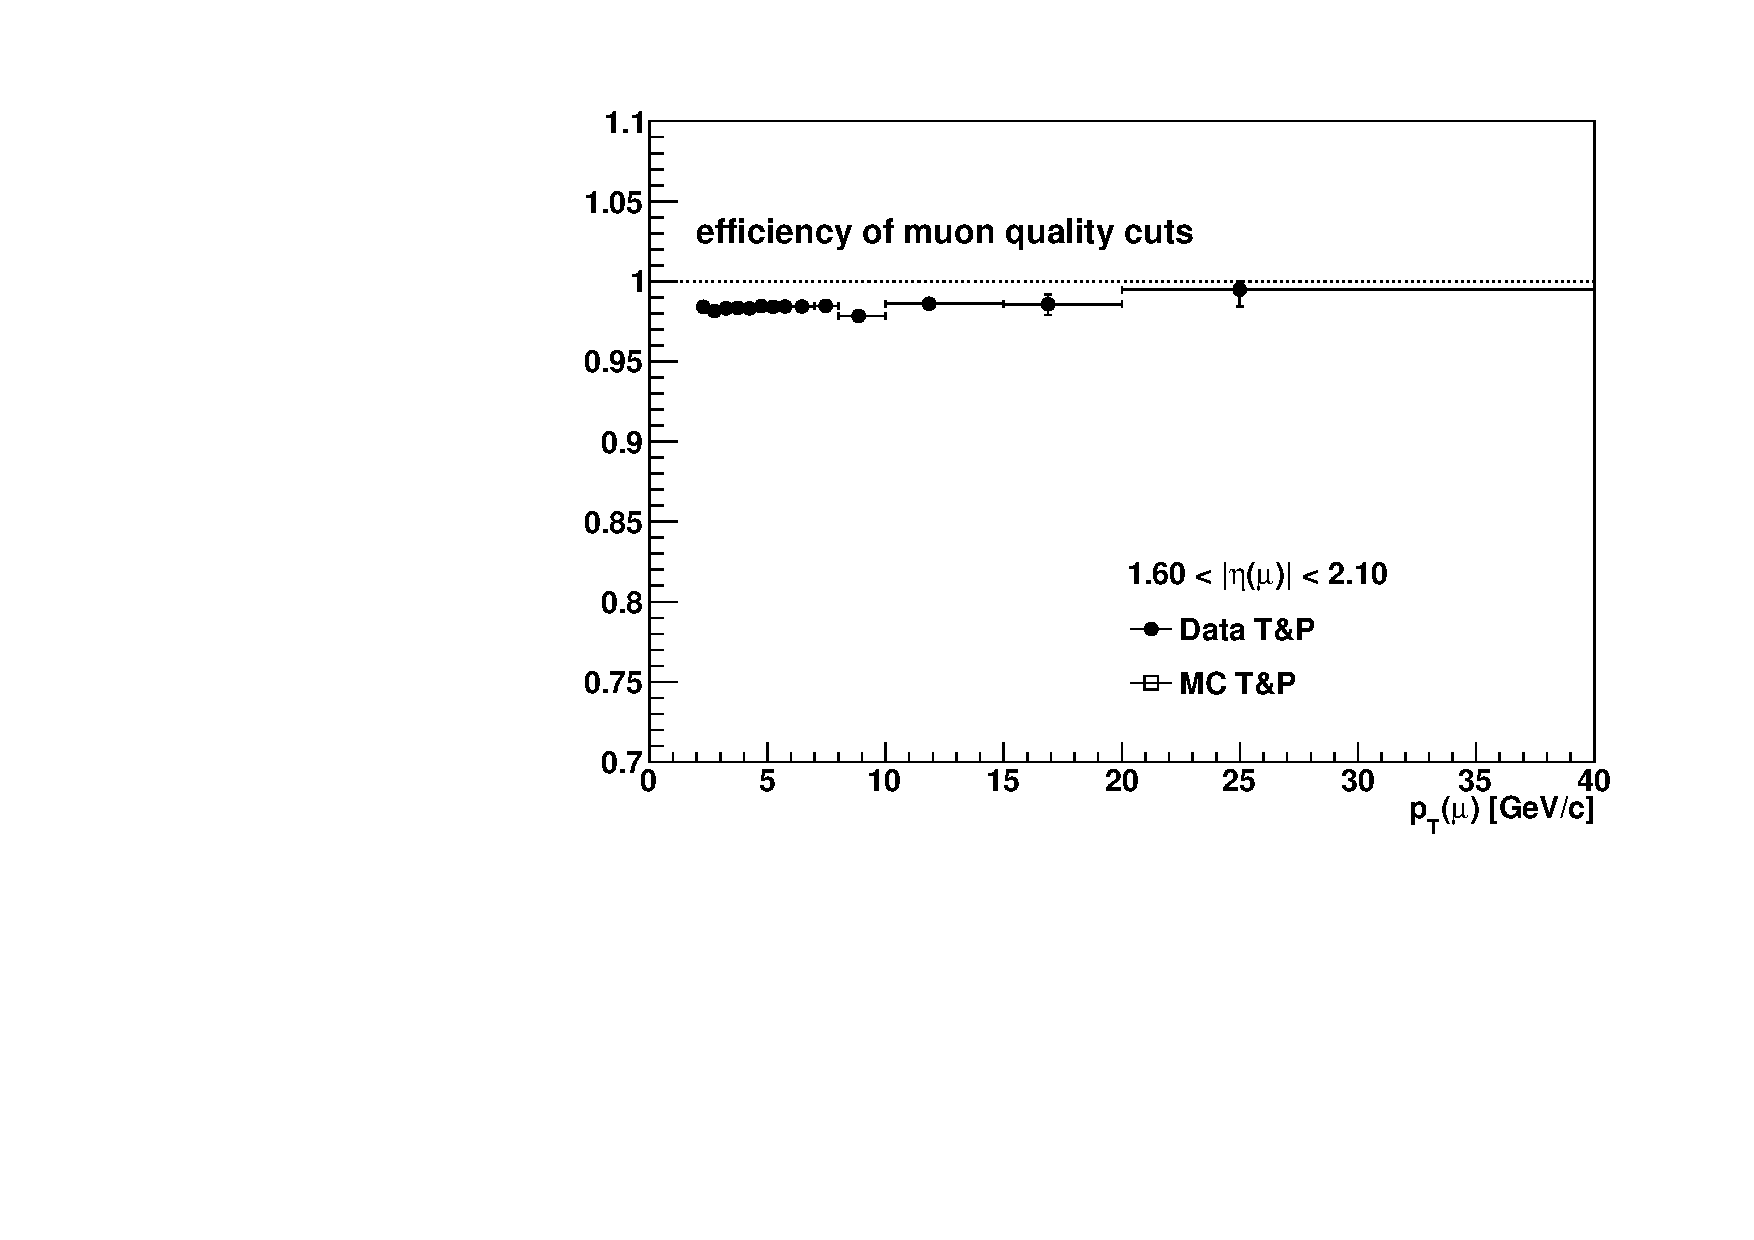
\includegraphics[width=0.49\textwidth]{Figures/\subDirName/MuQualEff_pT_DataVsMC_etaBin6.pdf}
%only for Tracker muon cuts
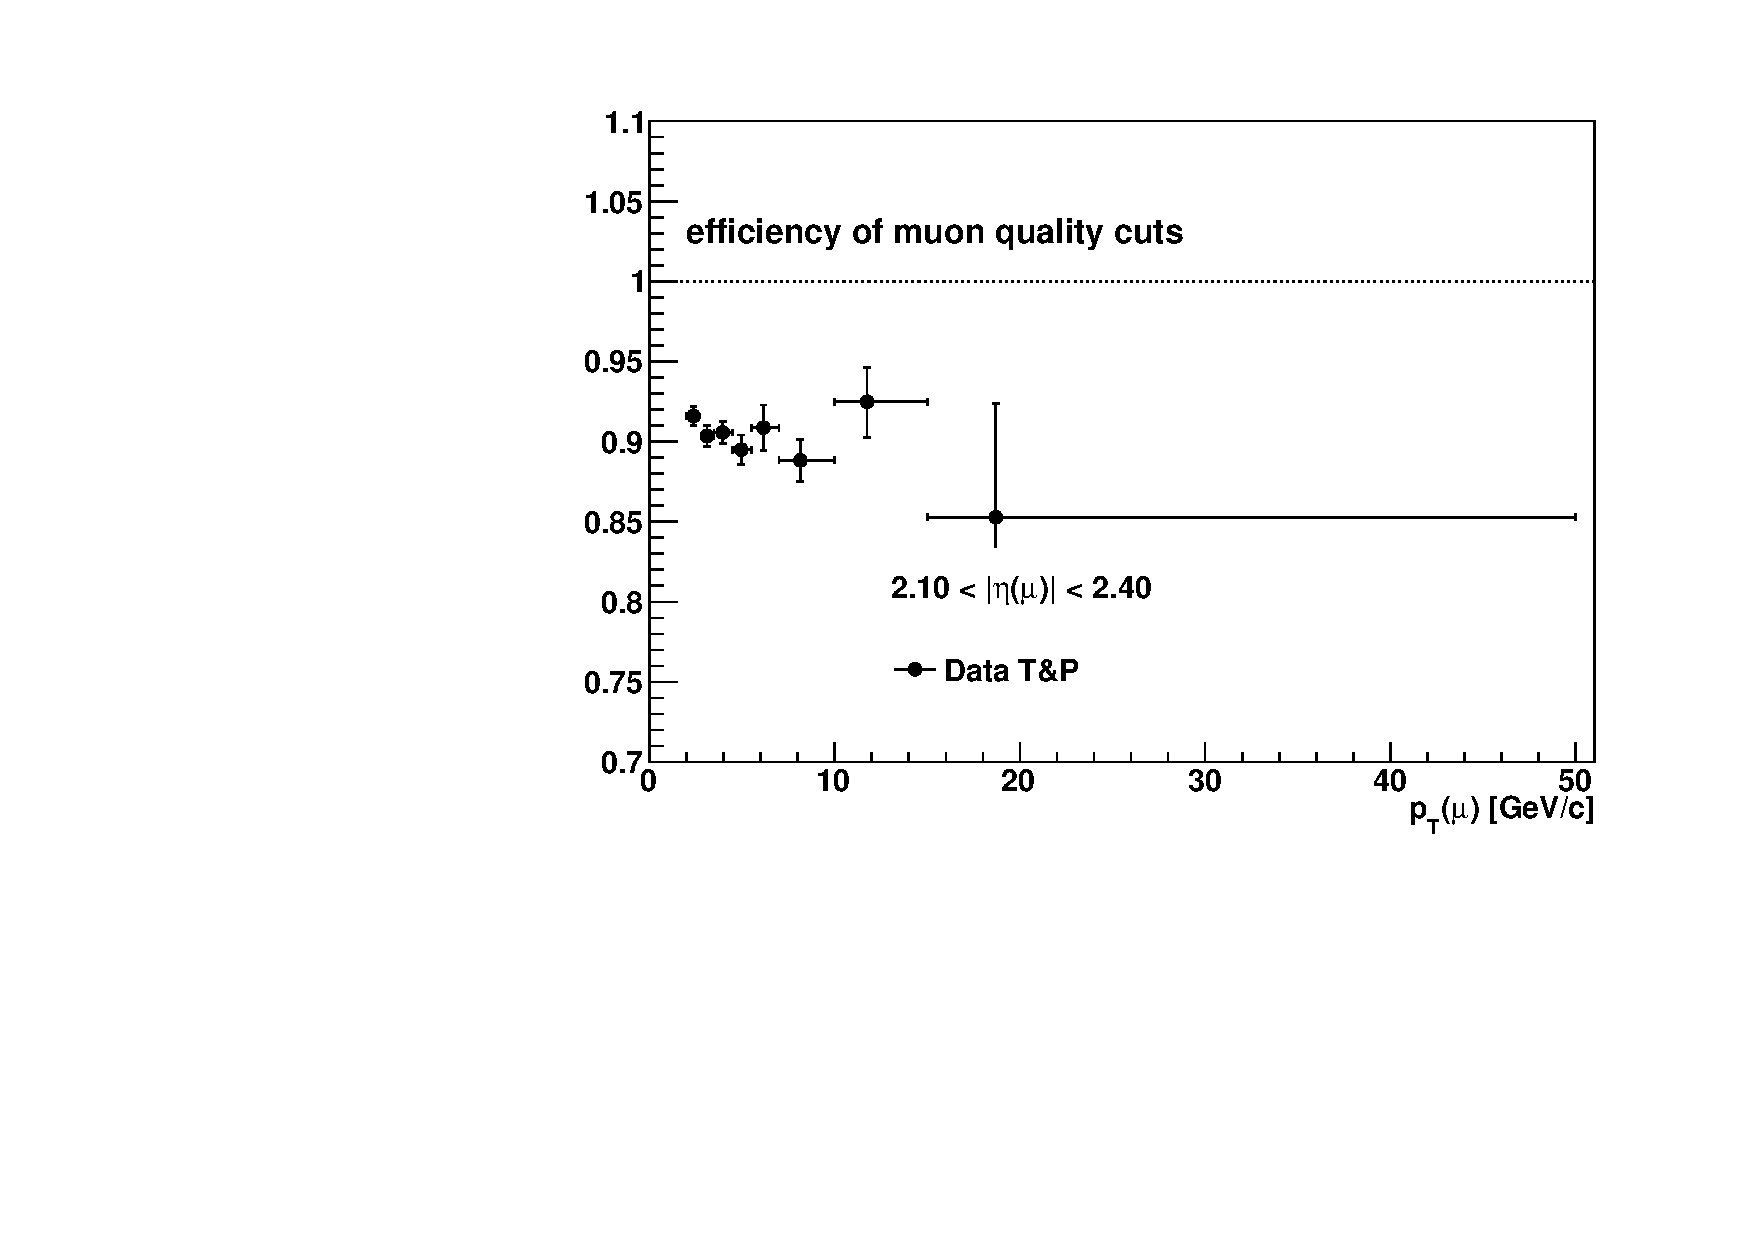
\includegraphics[width=0.49\textwidth]{Figures/\subDirName/MuQualEff_pT_DataVsMC_etaBin7.pdf}
\caption{Efficiency of the muon quality cuts versus \pt\ for small
  slices in $|\eta|$, using the ``tracker50'' muon cuts.}
\label{fig:muQualEff-pt}
\end{figure}
\begin{figure}[p]
\centering
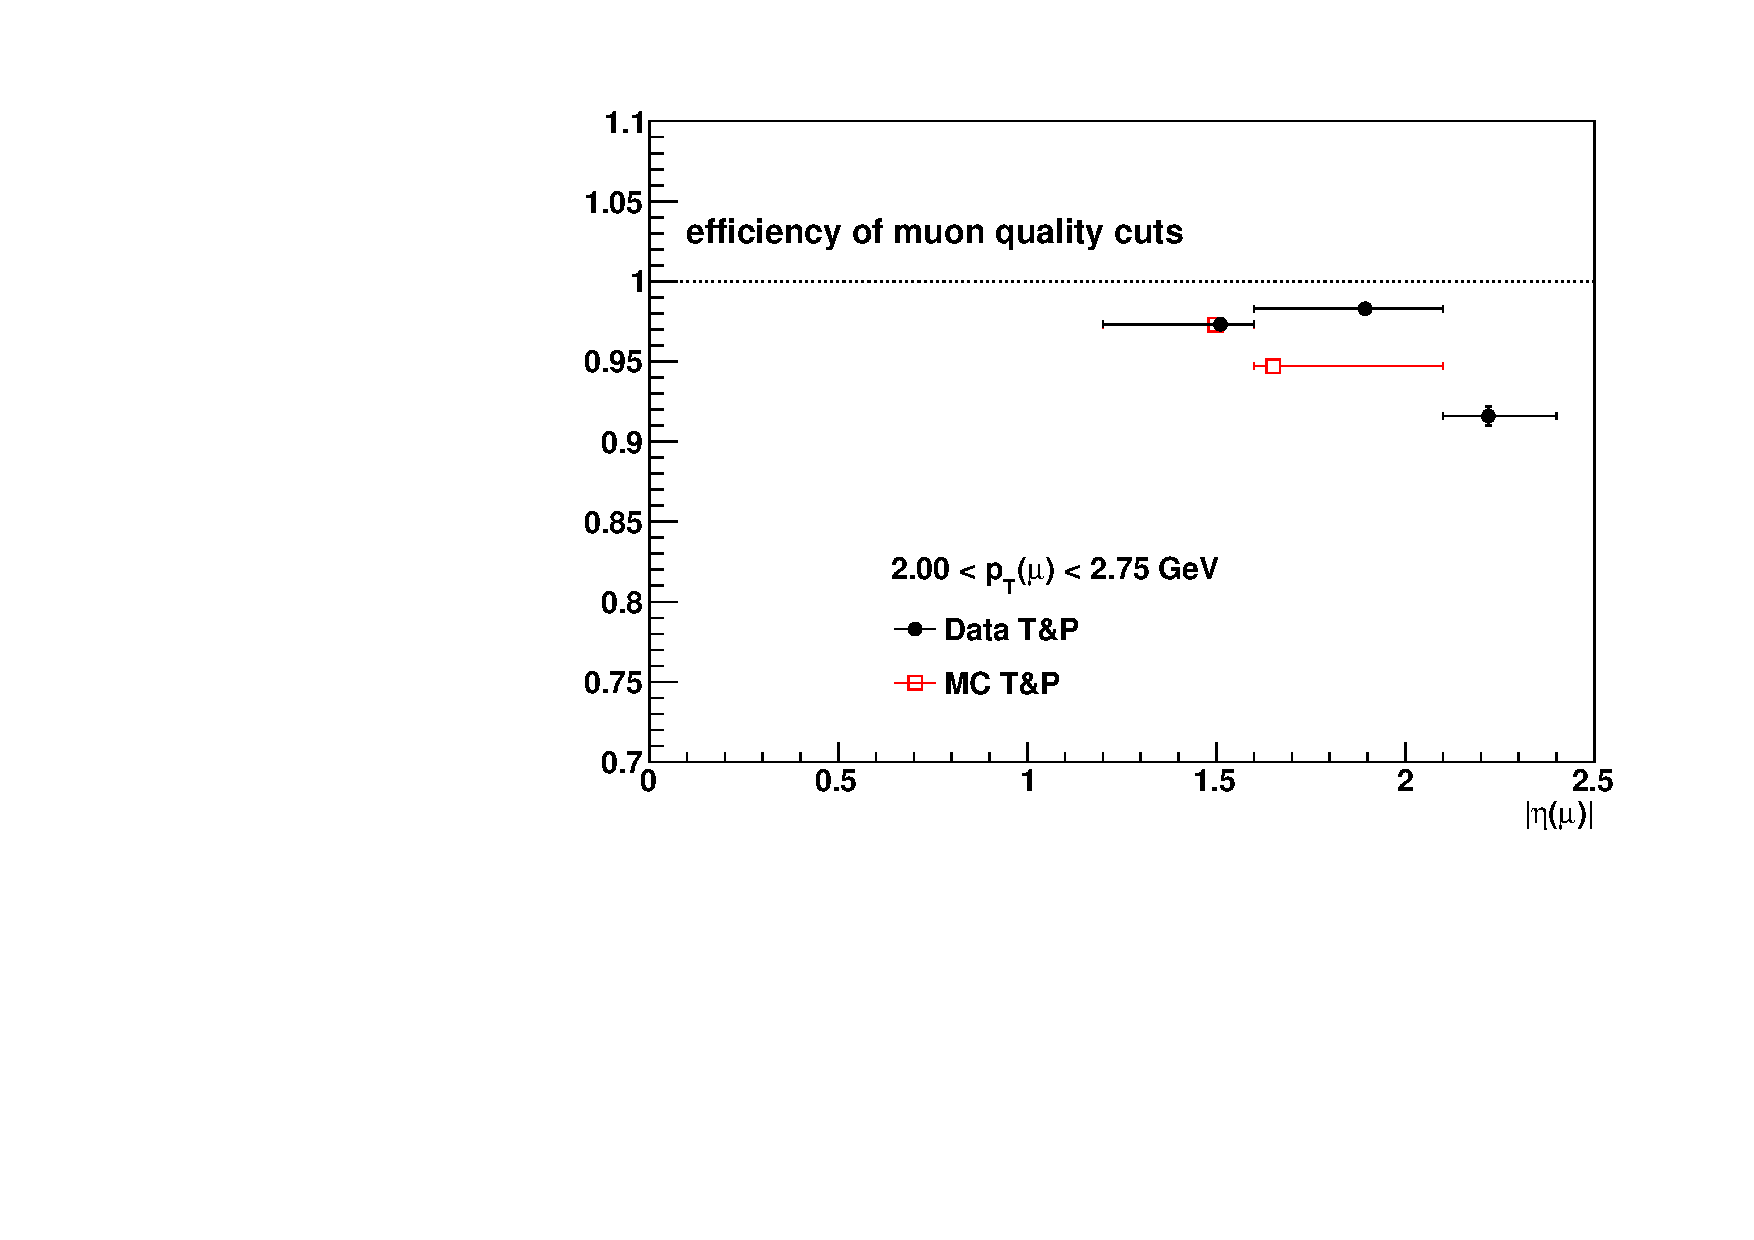
\includegraphics[width=0.49\textwidth]{Figures/\subDirName/MuQualEff_eta_DataVsMC_pTBin0.pdf}
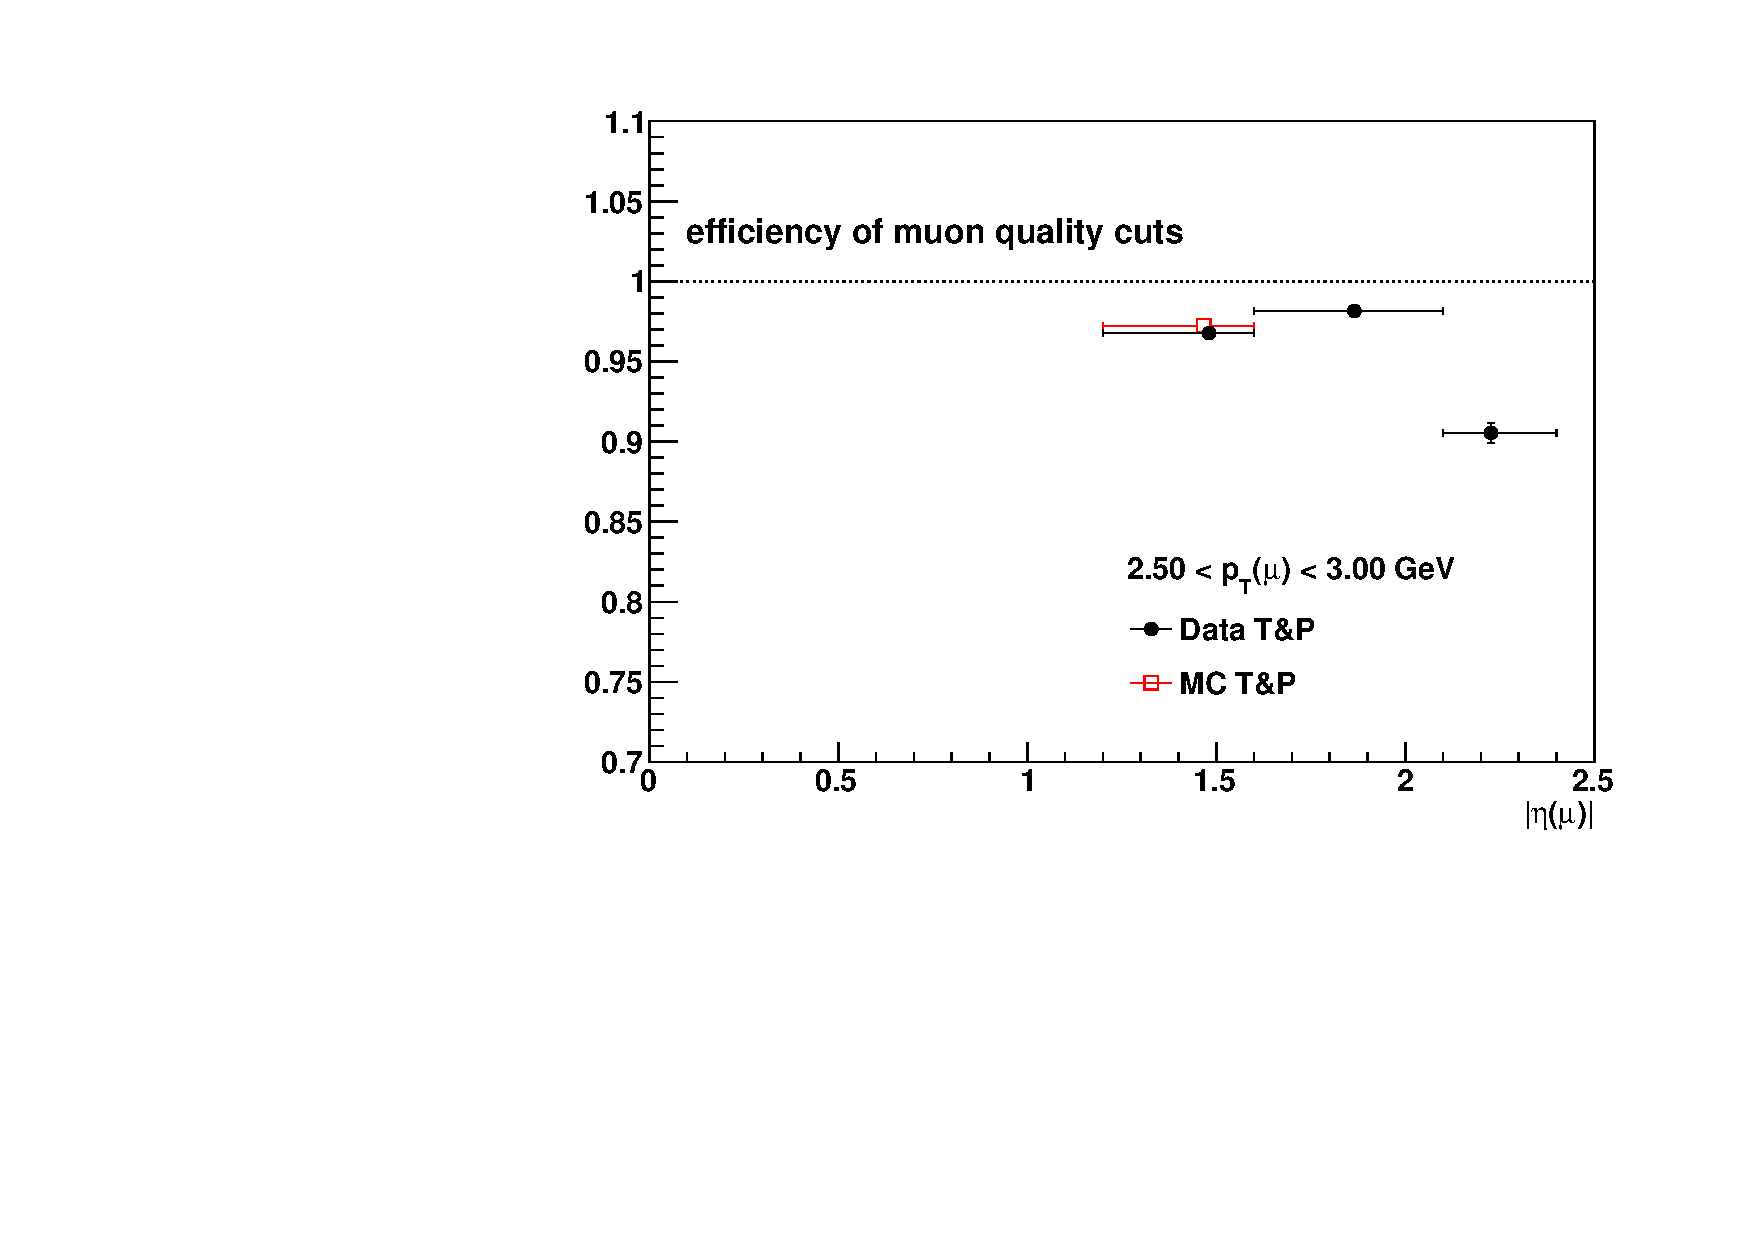
\includegraphics[width=0.49\textwidth]{Figures/\subDirName/MuQualEff_eta_DataVsMC_pTBin1.pdf}
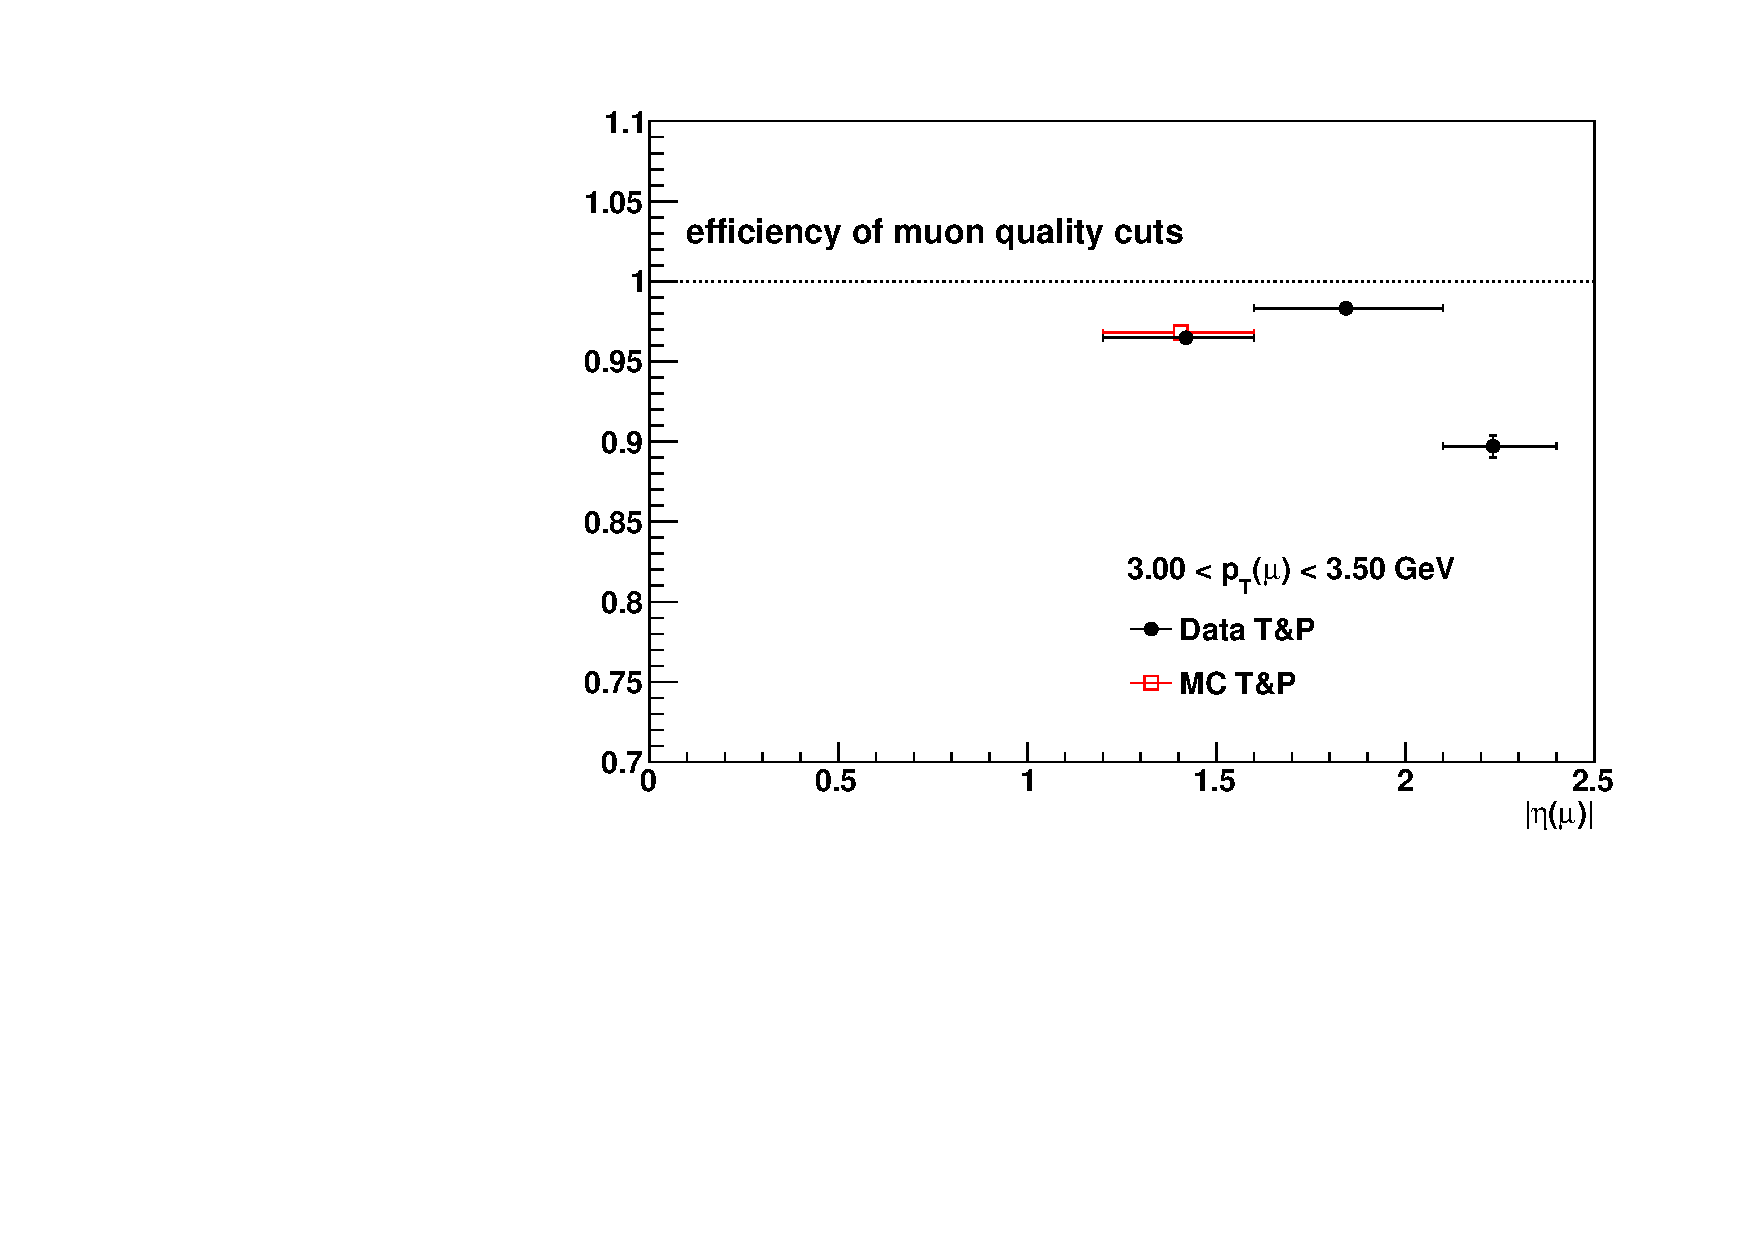
\includegraphics[width=0.49\textwidth]{Figures/\subDirName/MuQualEff_eta_DataVsMC_pTBin2.pdf}
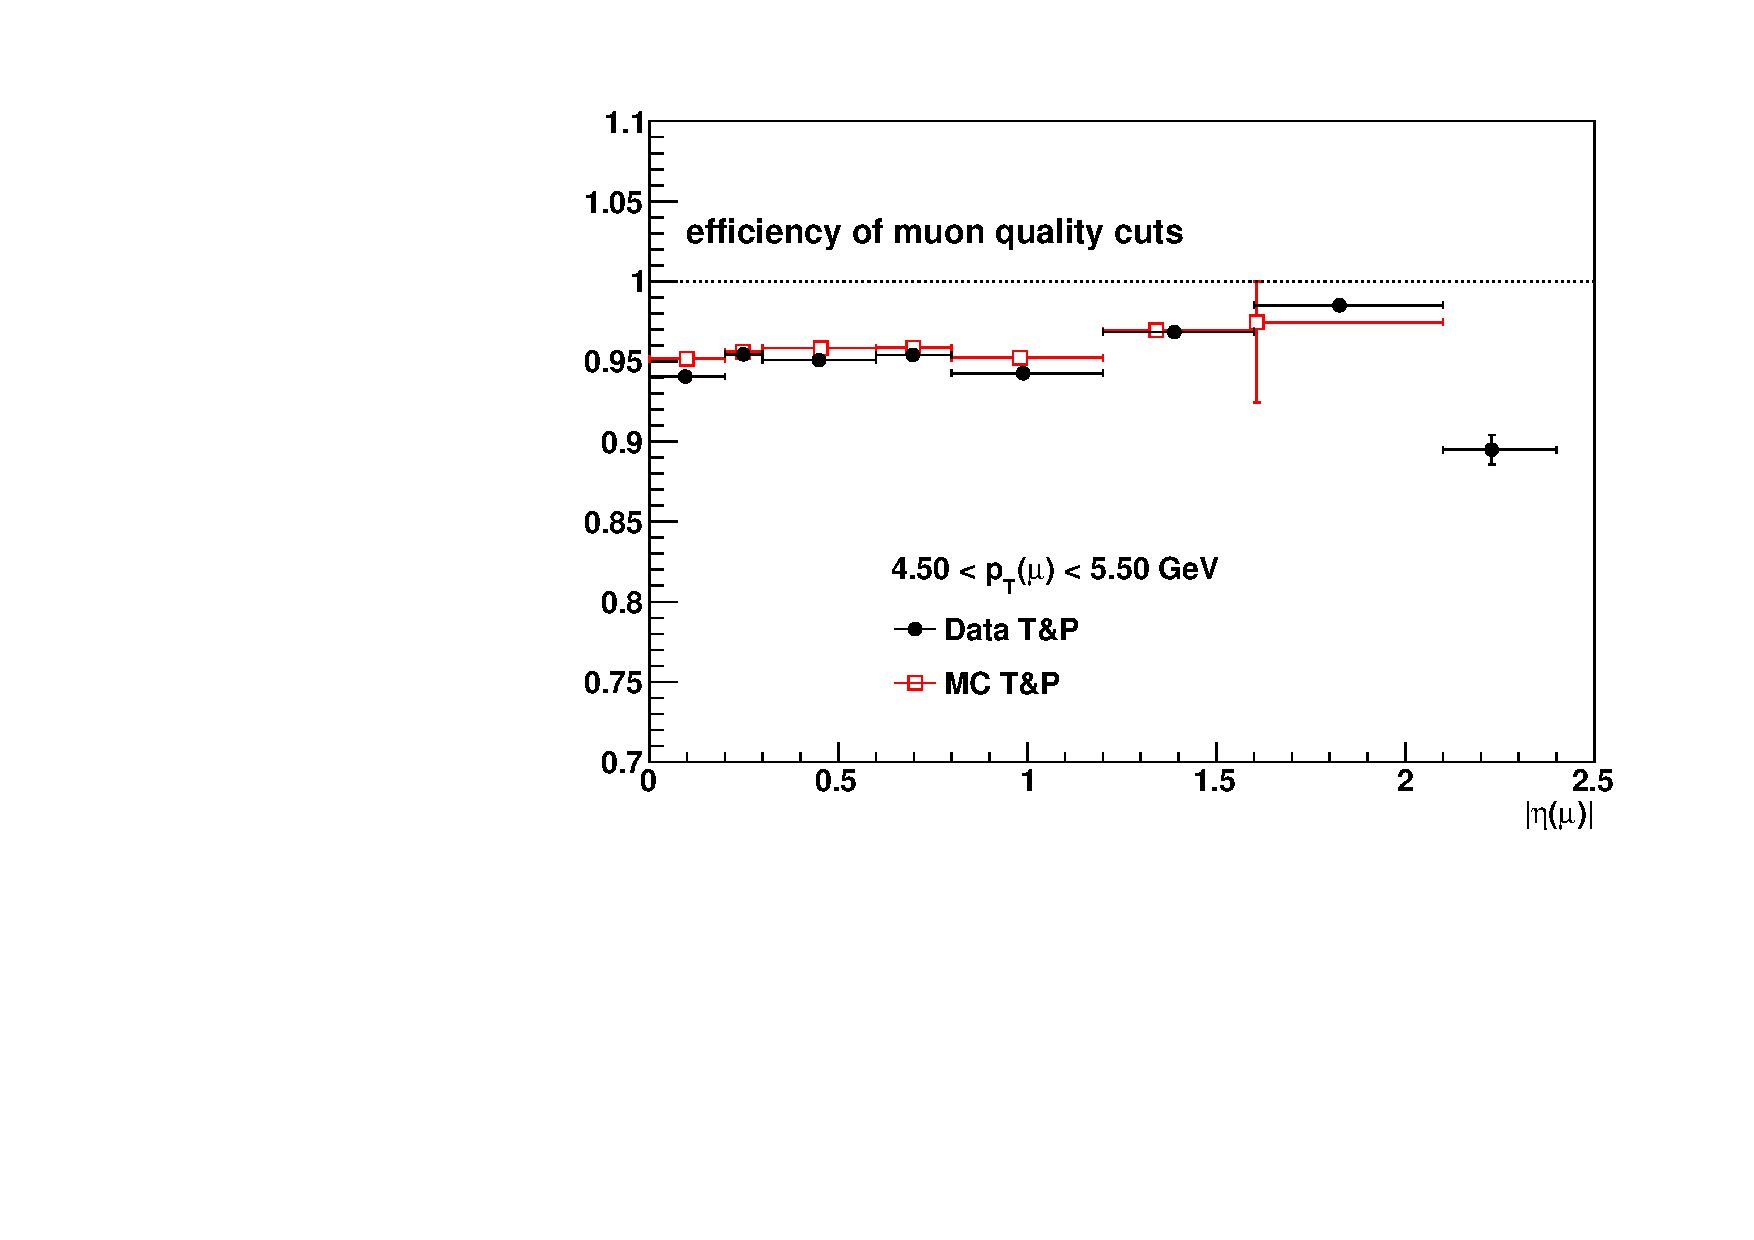
\includegraphics[width=0.49\textwidth]{Figures/\subDirName/MuQualEff_eta_DataVsMC_pTBin3.pdf}
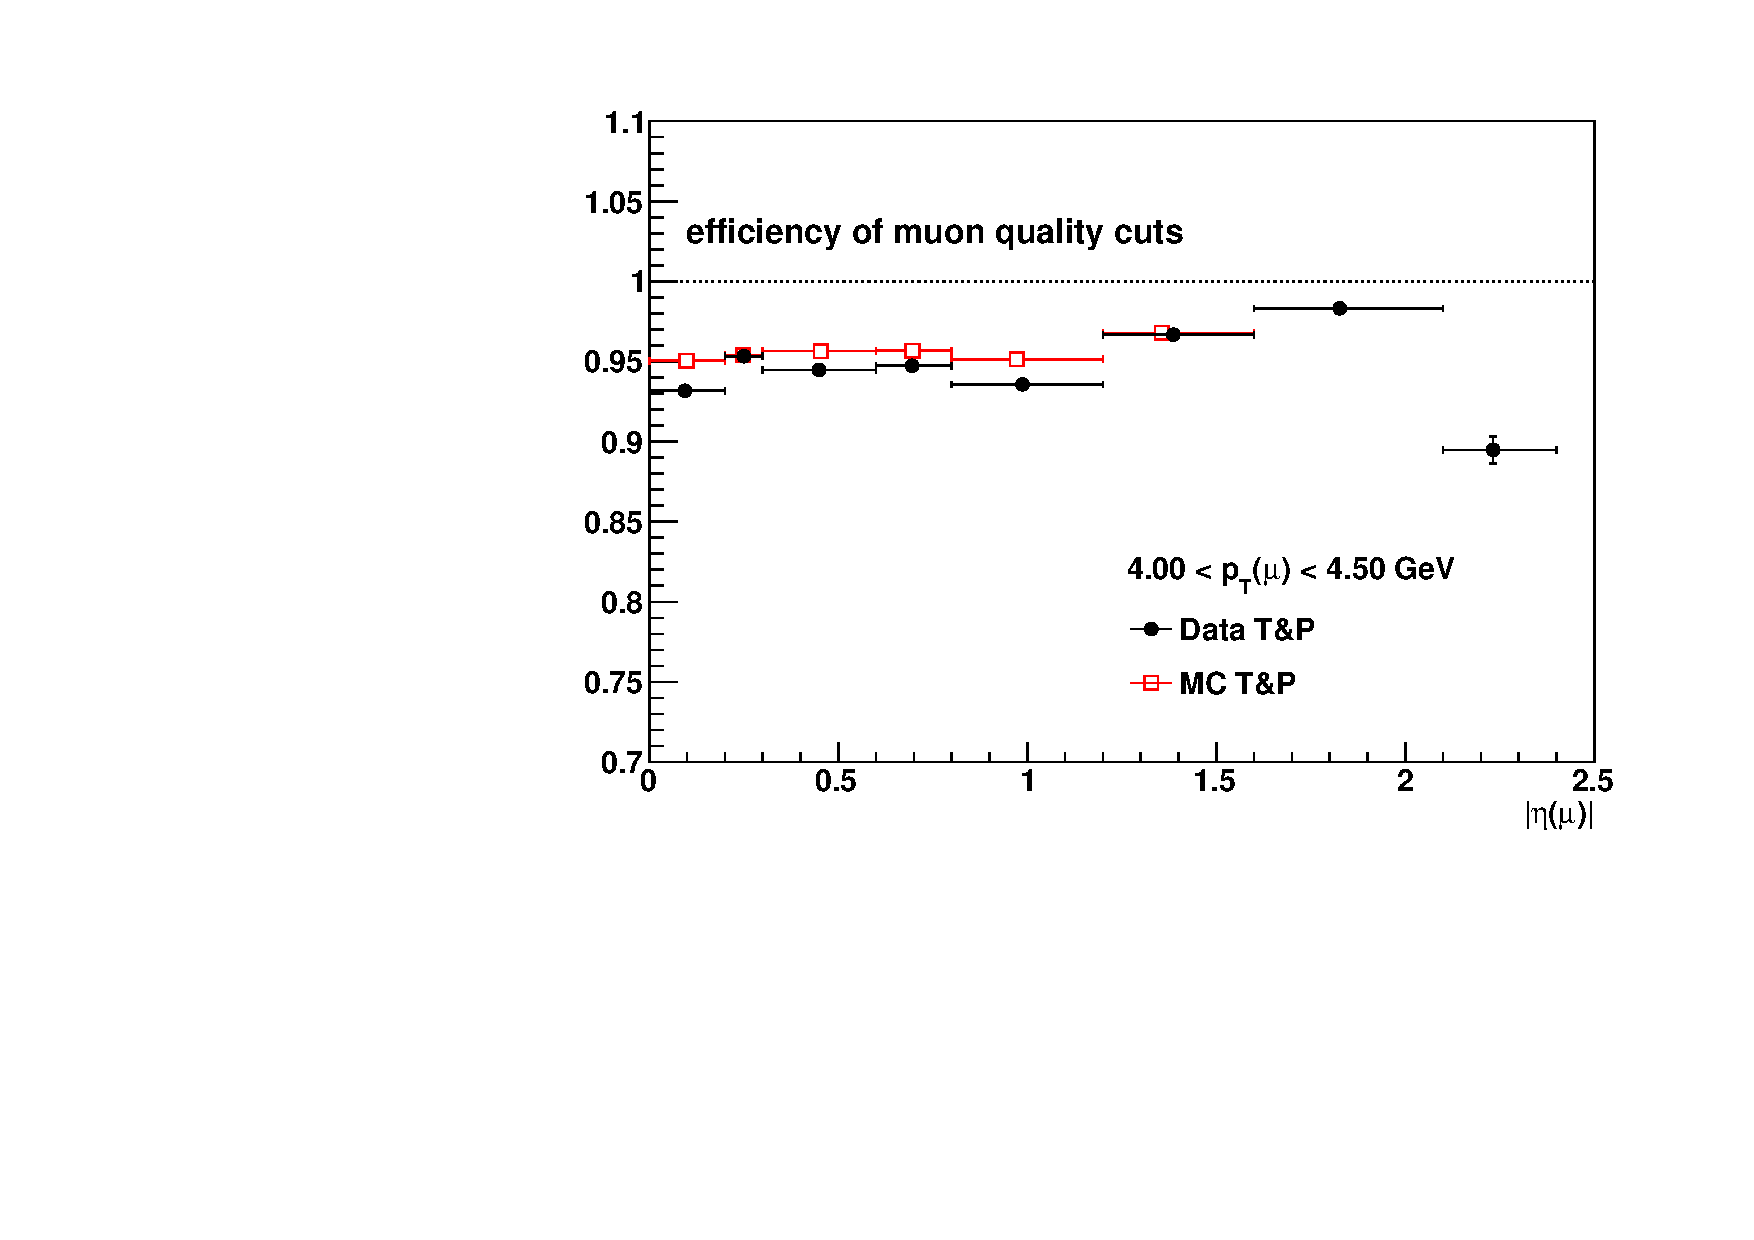
\includegraphics[width=0.49\textwidth]{Figures/\subDirName/MuQualEff_eta_DataVsMC_pTBin4.pdf}
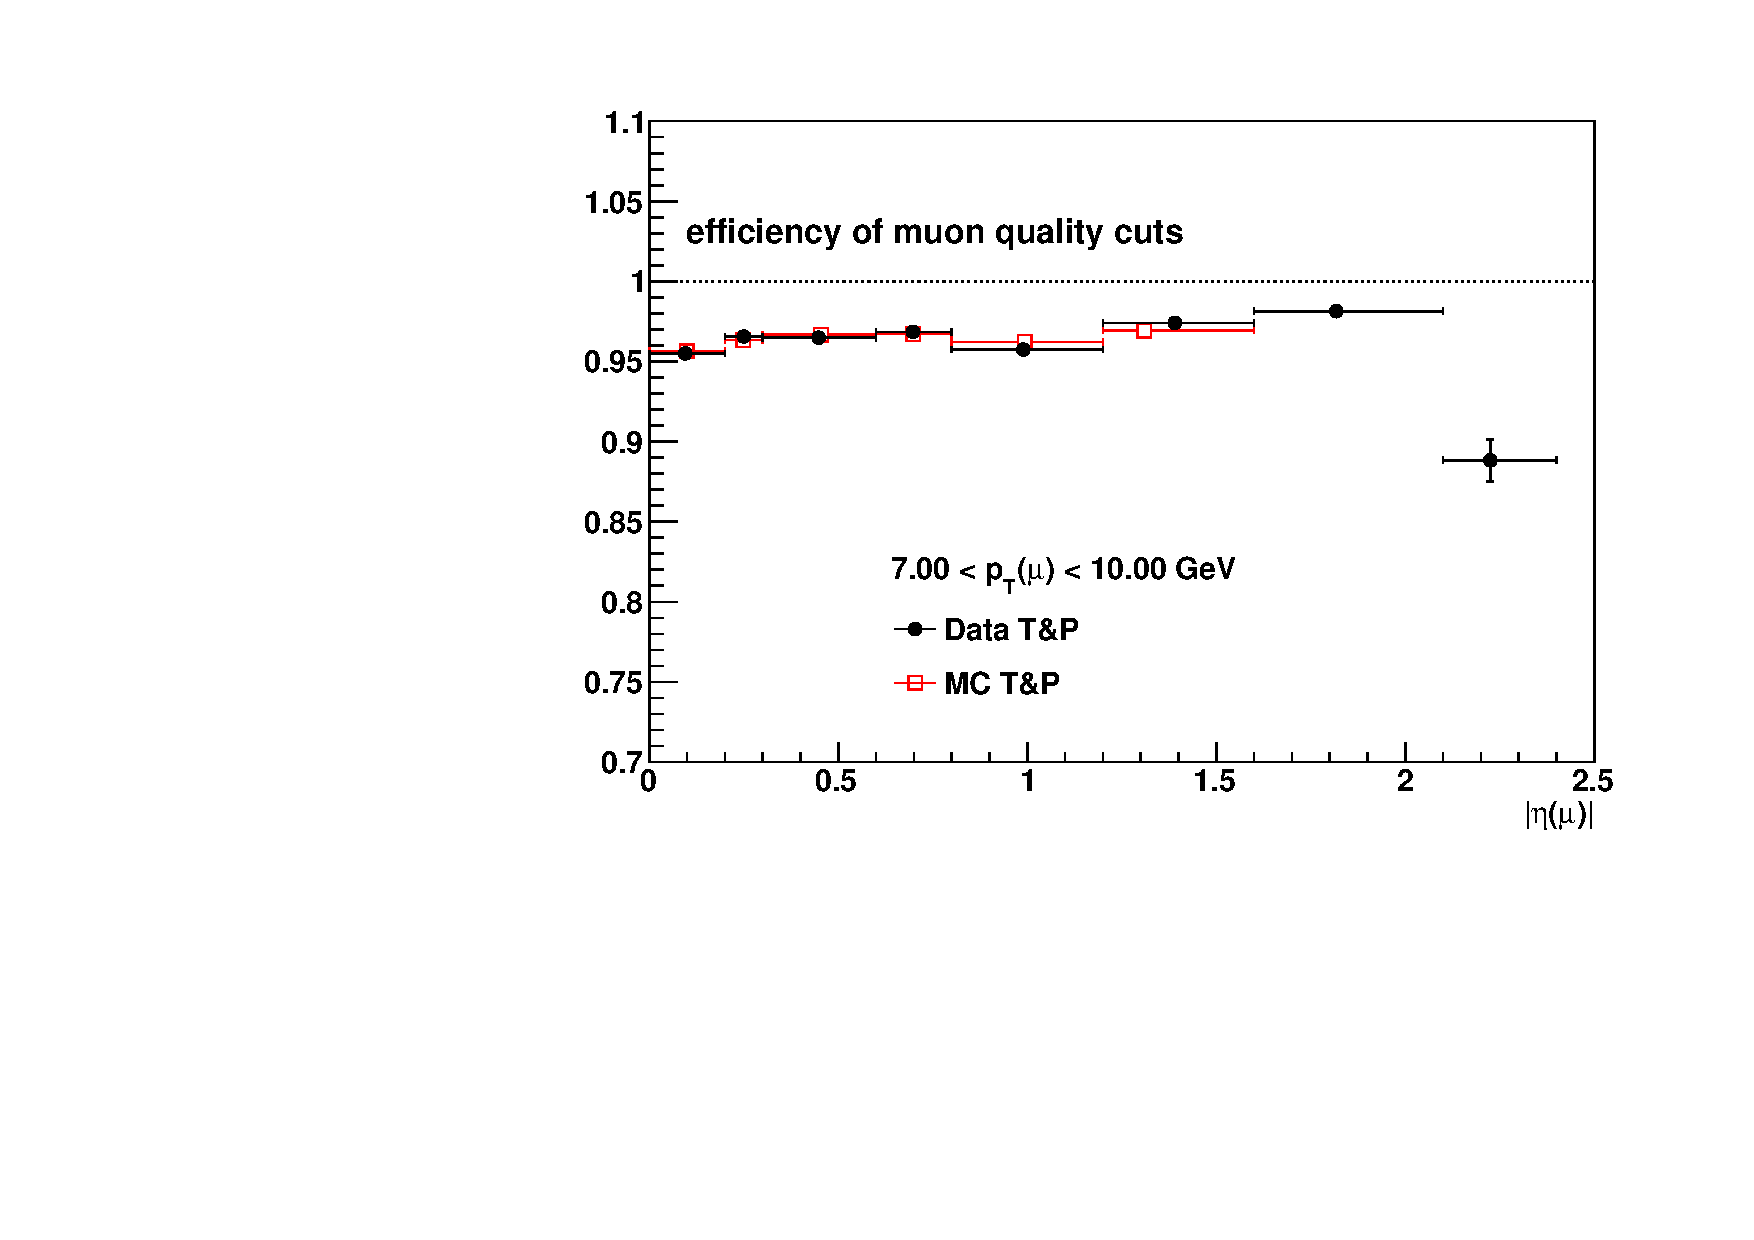
\includegraphics[width=0.49\textwidth]{Figures/\subDirName/MuQualEff_eta_DataVsMC_pTBin5.pdf}
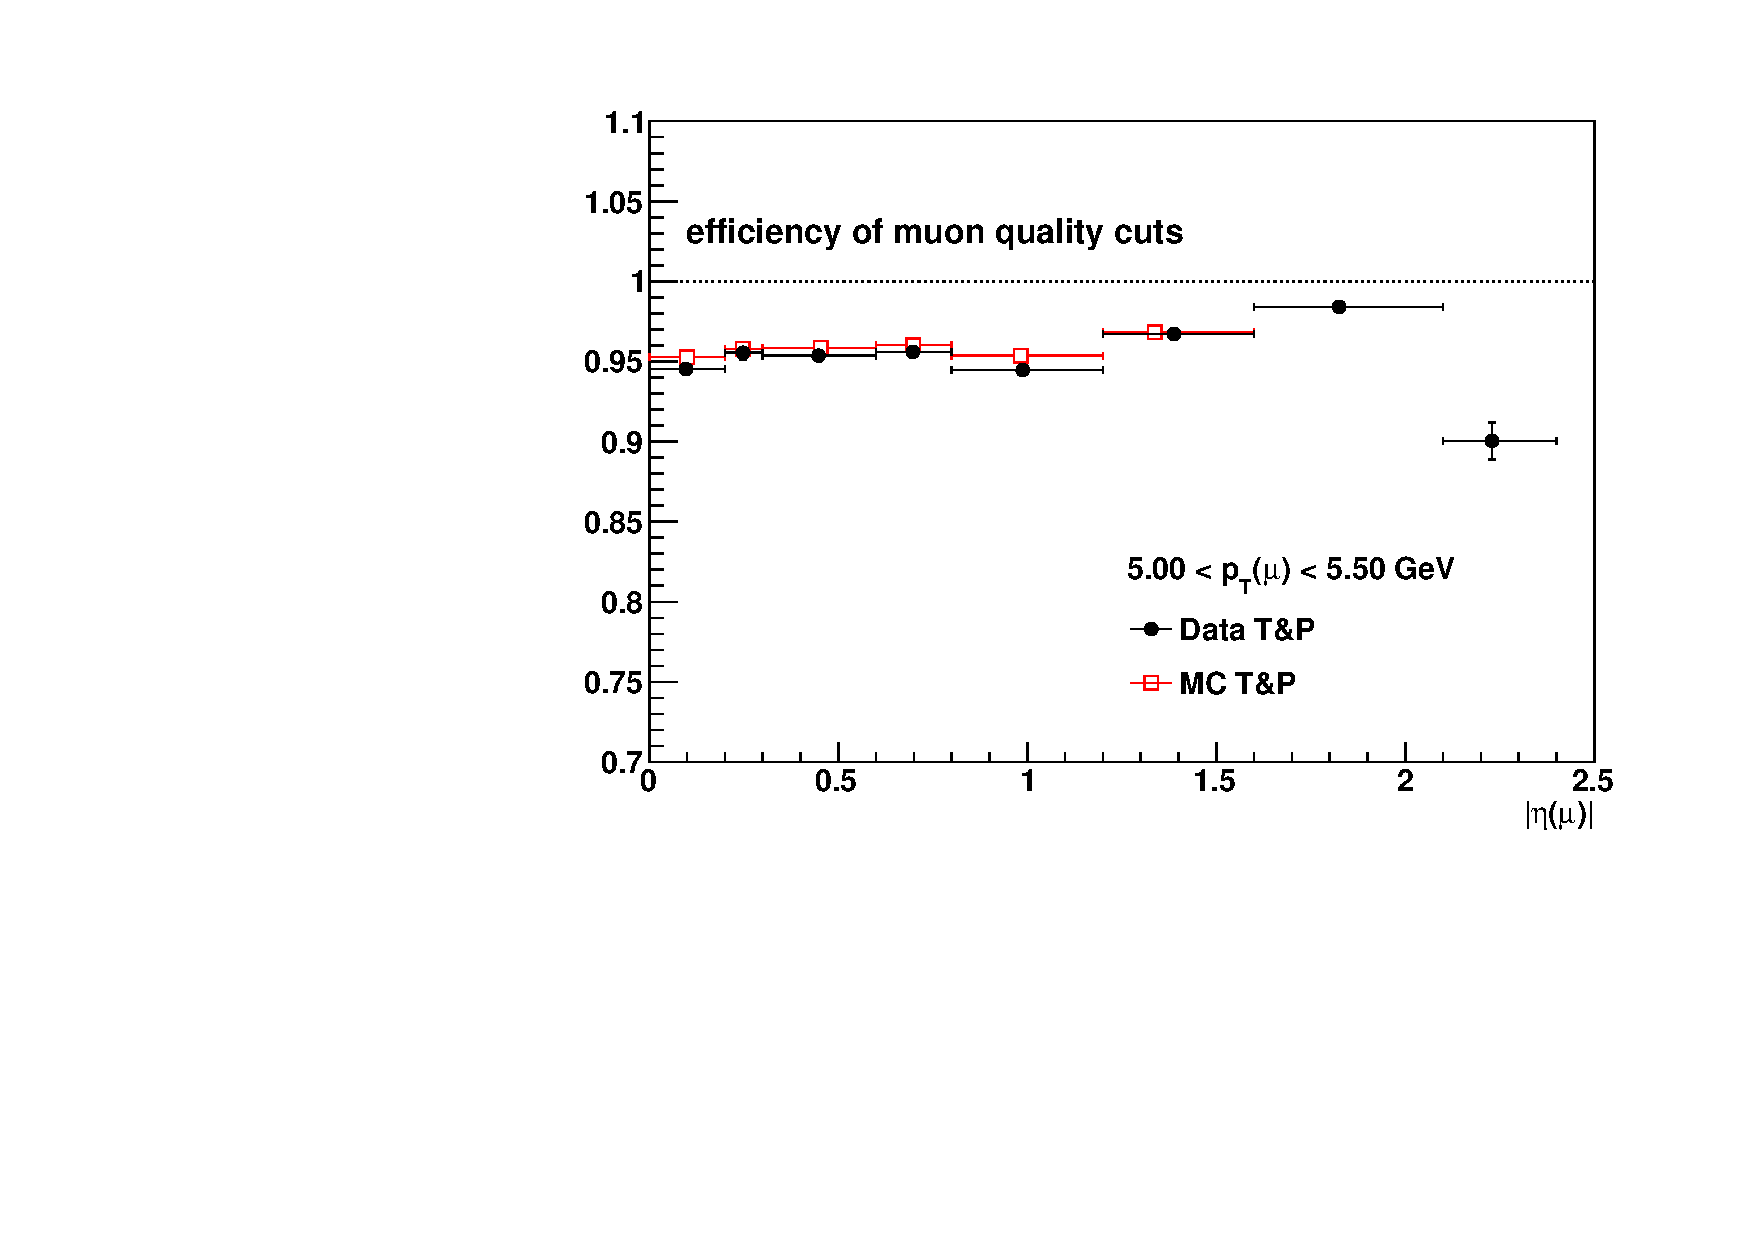
\includegraphics[width=0.49\textwidth]{Figures/\subDirName/MuQualEff_eta_DataVsMC_pTBin6.pdf}
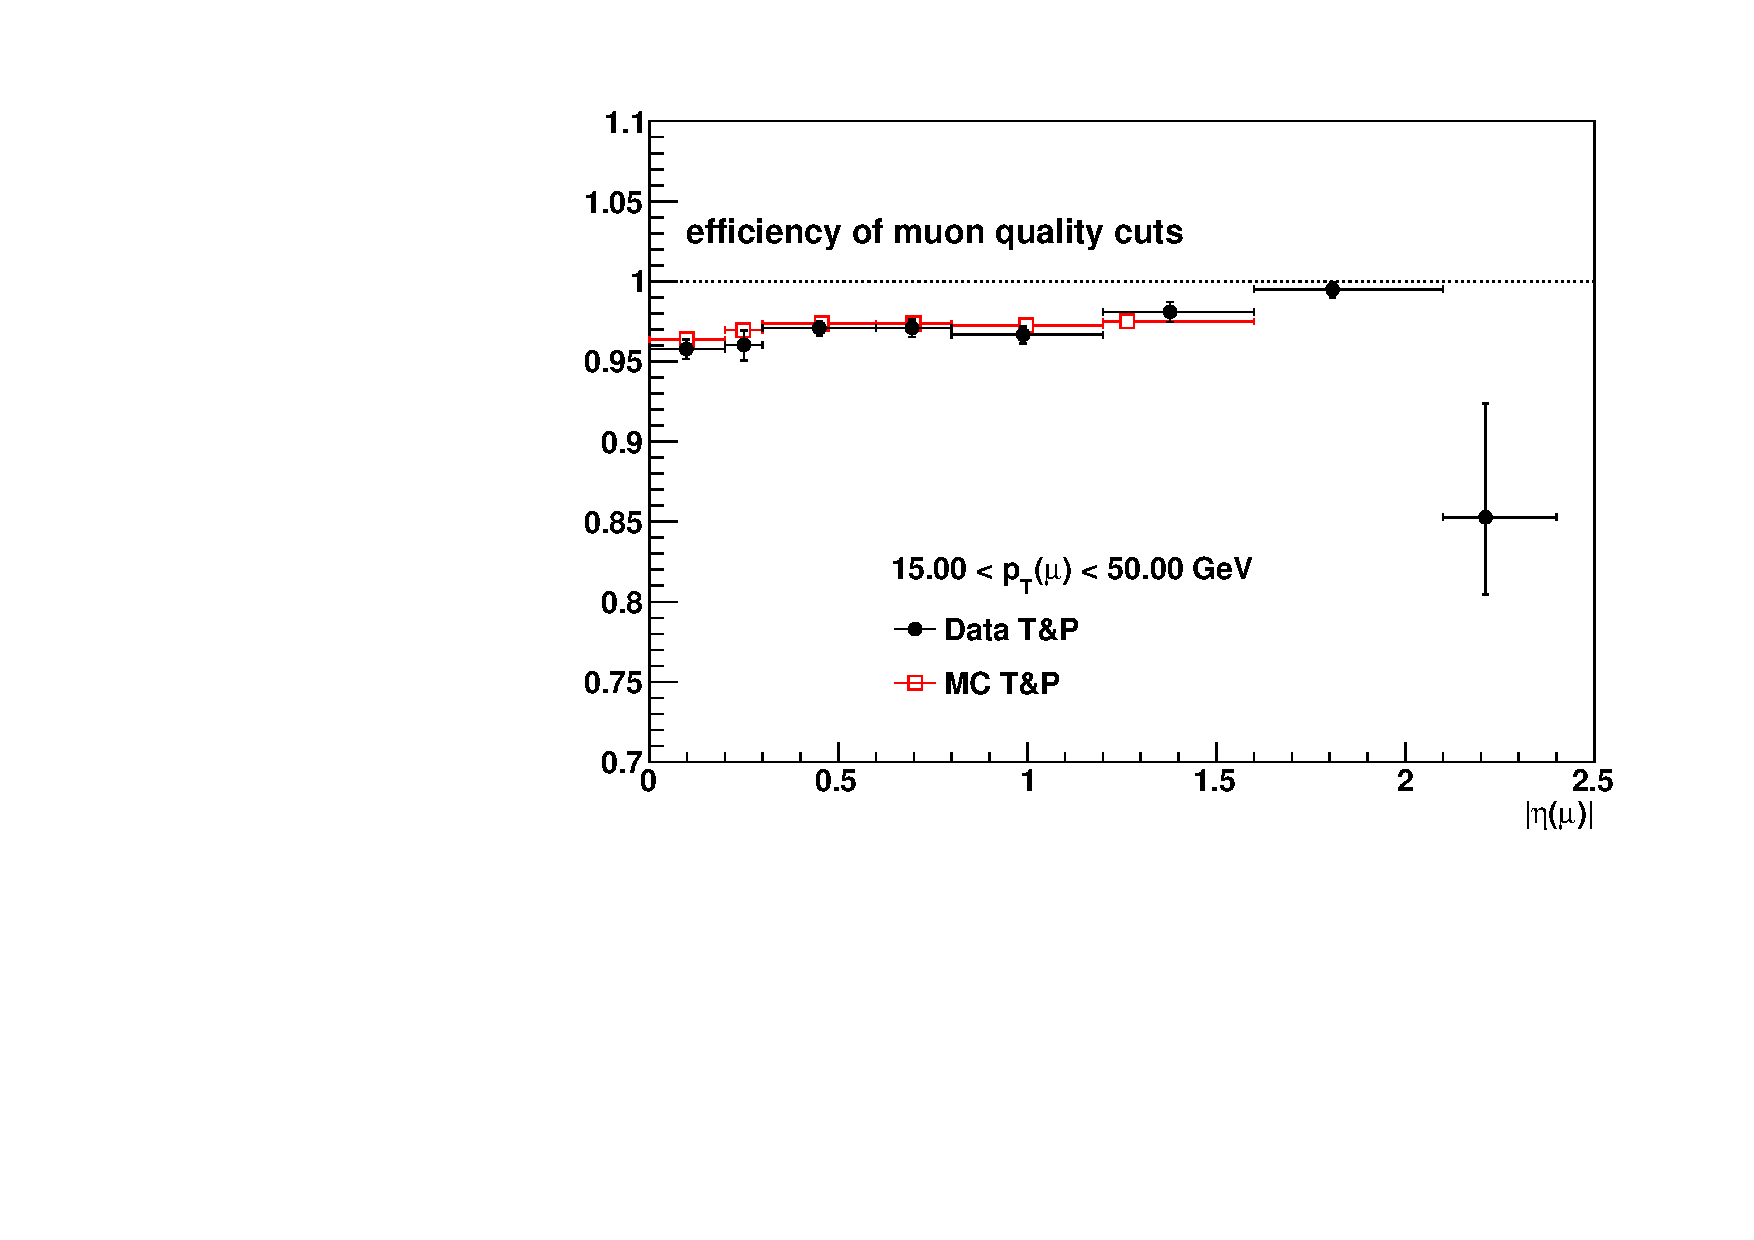
\includegraphics[width=0.49\textwidth]{Figures/\subDirName/MuQualEff_eta_DataVsMC_pTBin7.pdf}
\caption{Efficiency of the muon quality cuts, versus $|\eta|$ for
  small slices in \pt, using the ``tracker50'' muon cuts.}
\label{fig:muQualEff-eta-1}
\end{figure}
\begin{figure}[p]
\centering
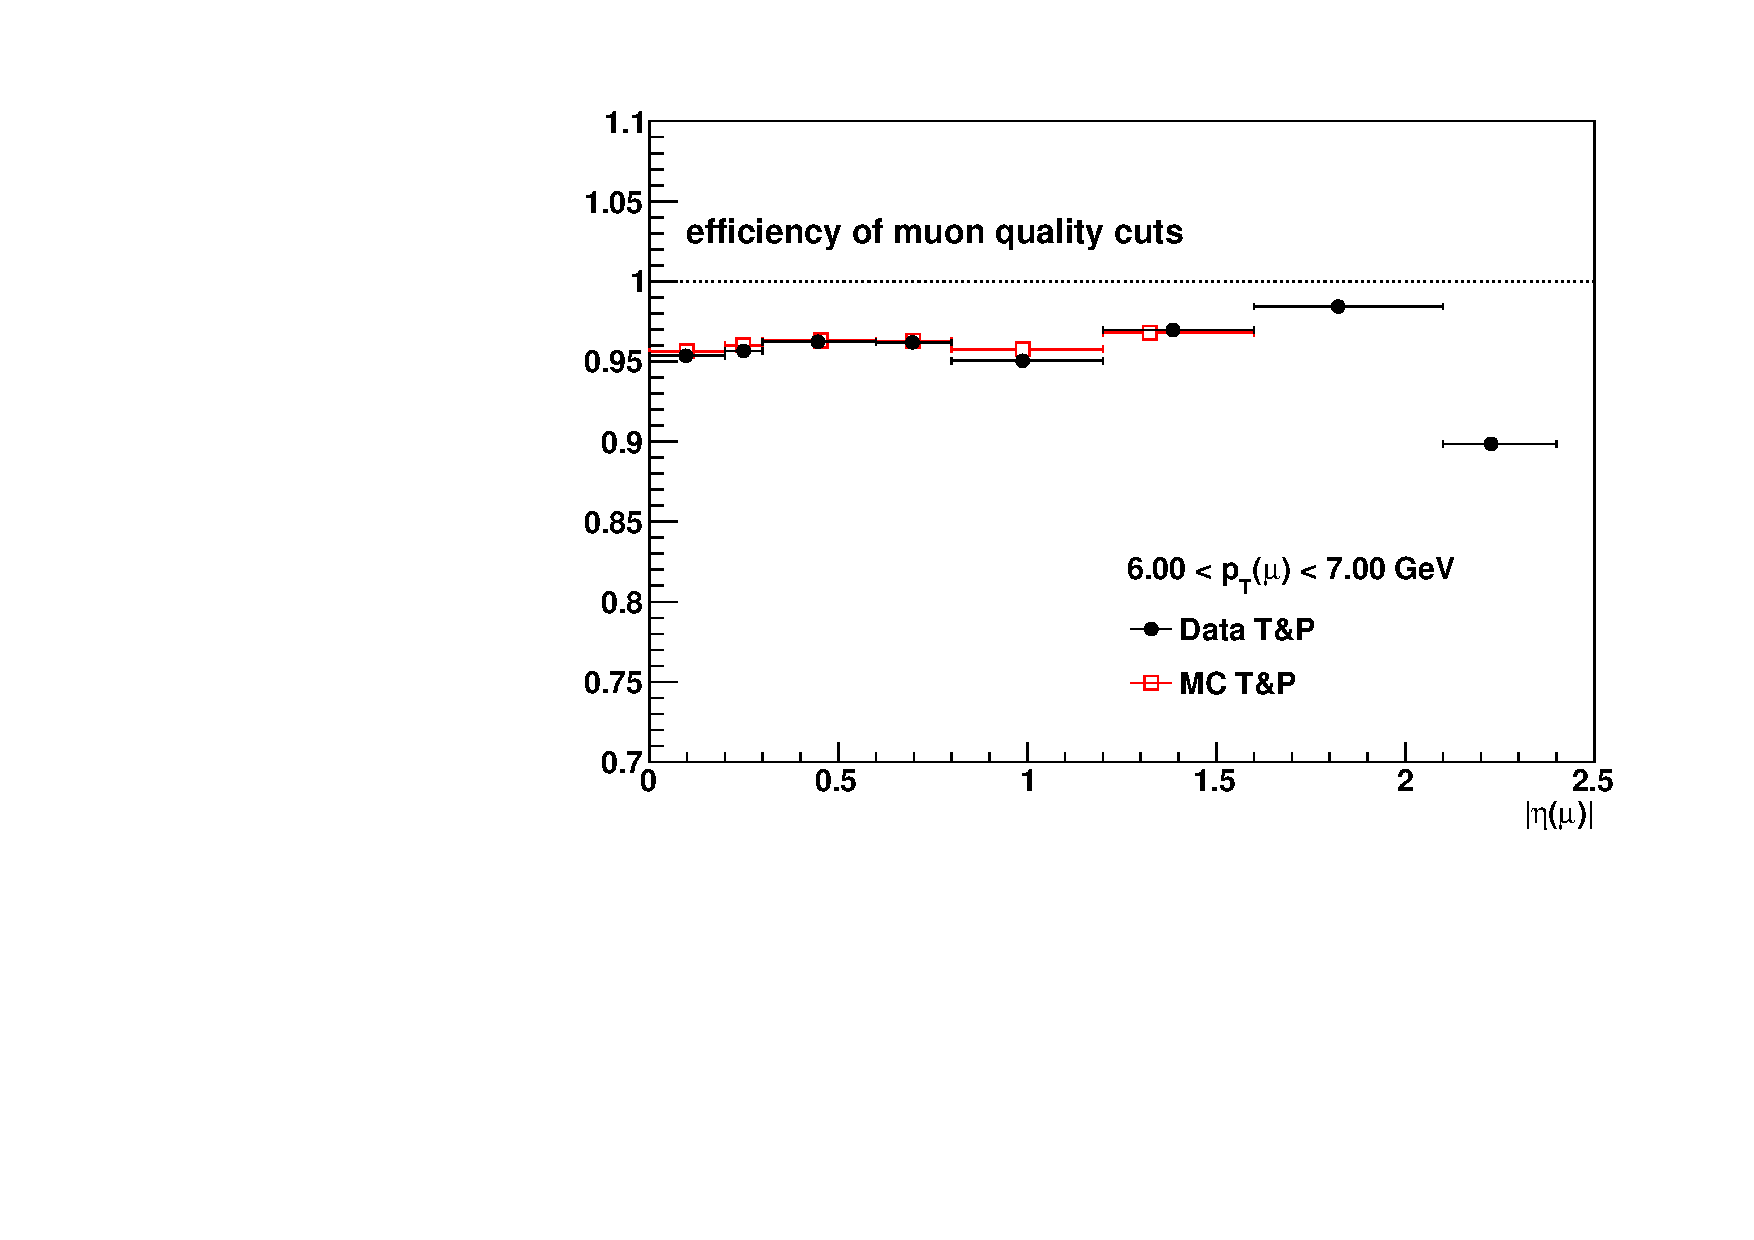
\includegraphics[width=0.49\textwidth]{Figures/\subDirName/MuQualEff_eta_DataVsMC_pTBin8.pdf}
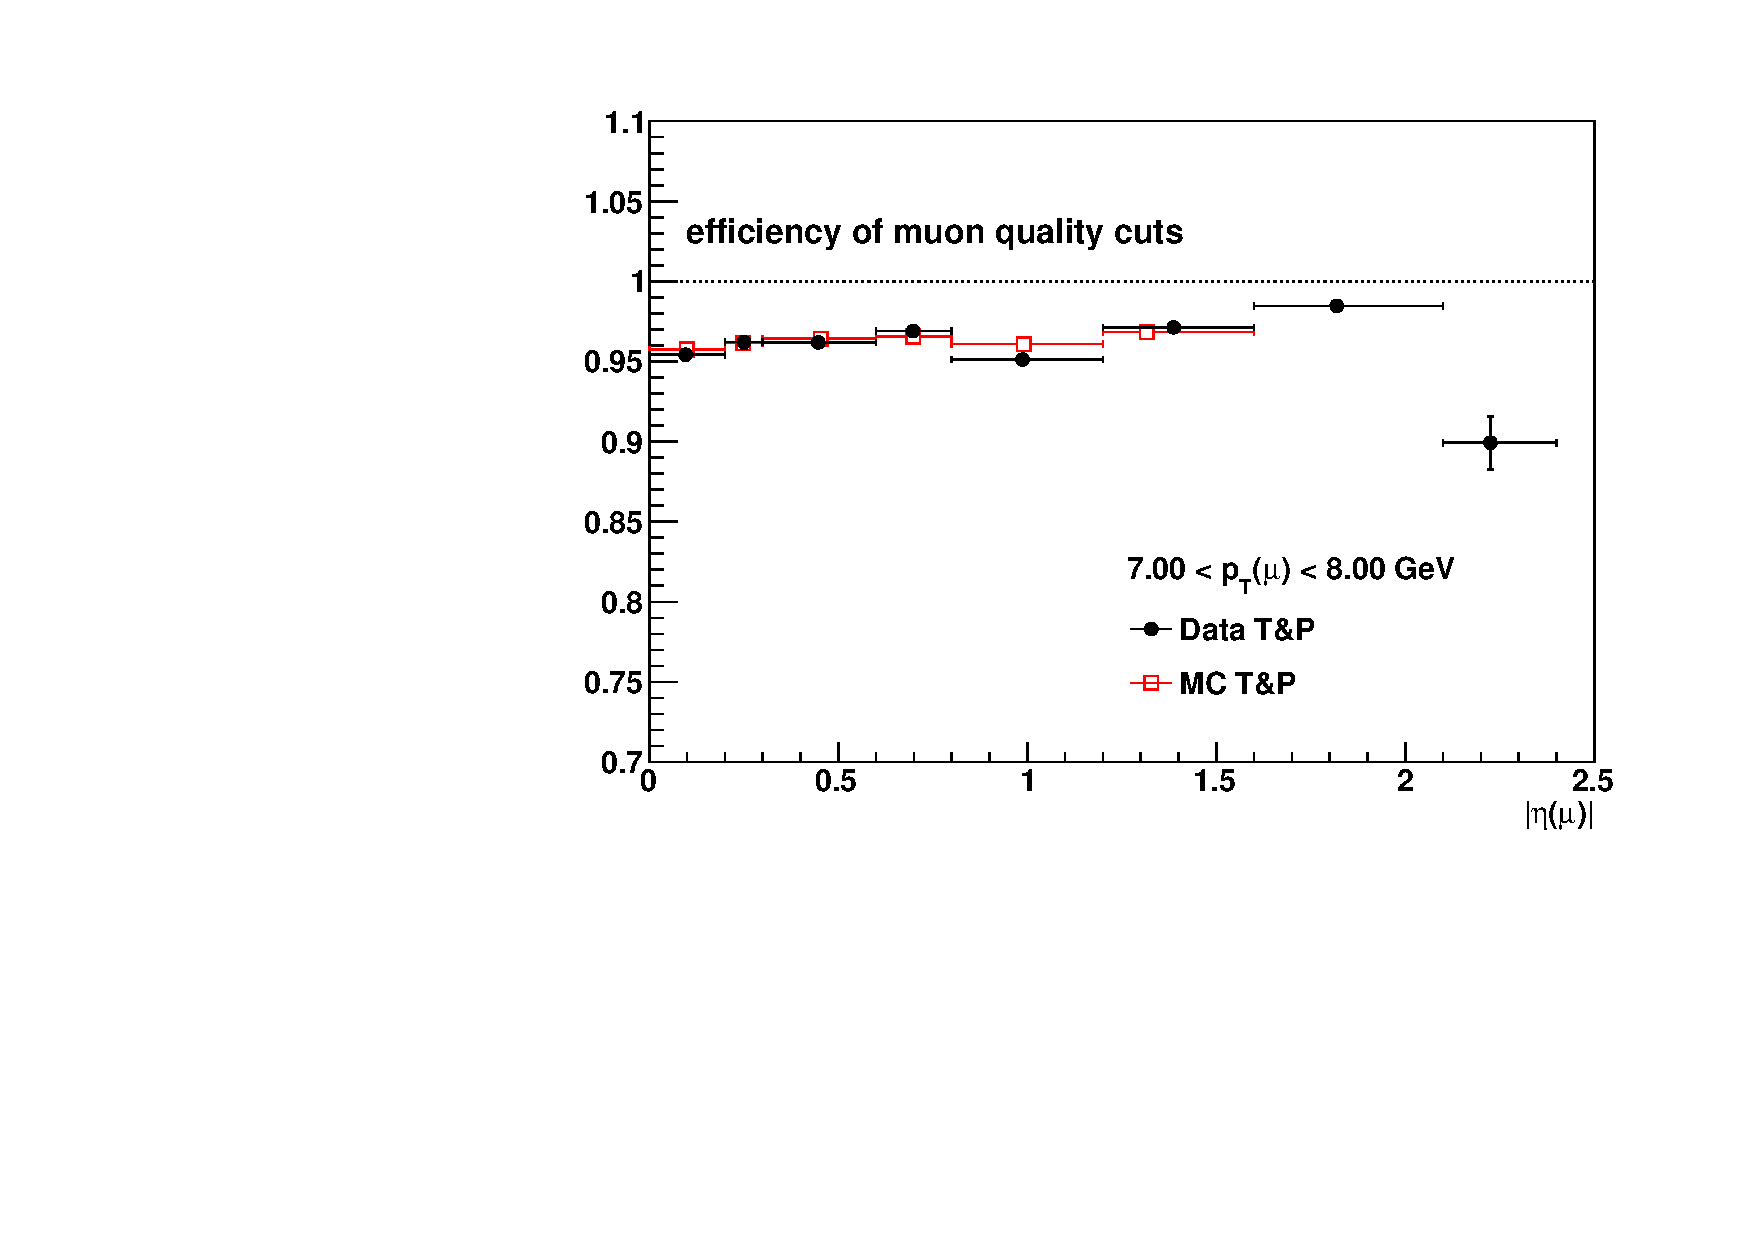
\includegraphics[width=0.49\textwidth]{Figures/\subDirName/MuQualEff_eta_DataVsMC_pTBin9.pdf}
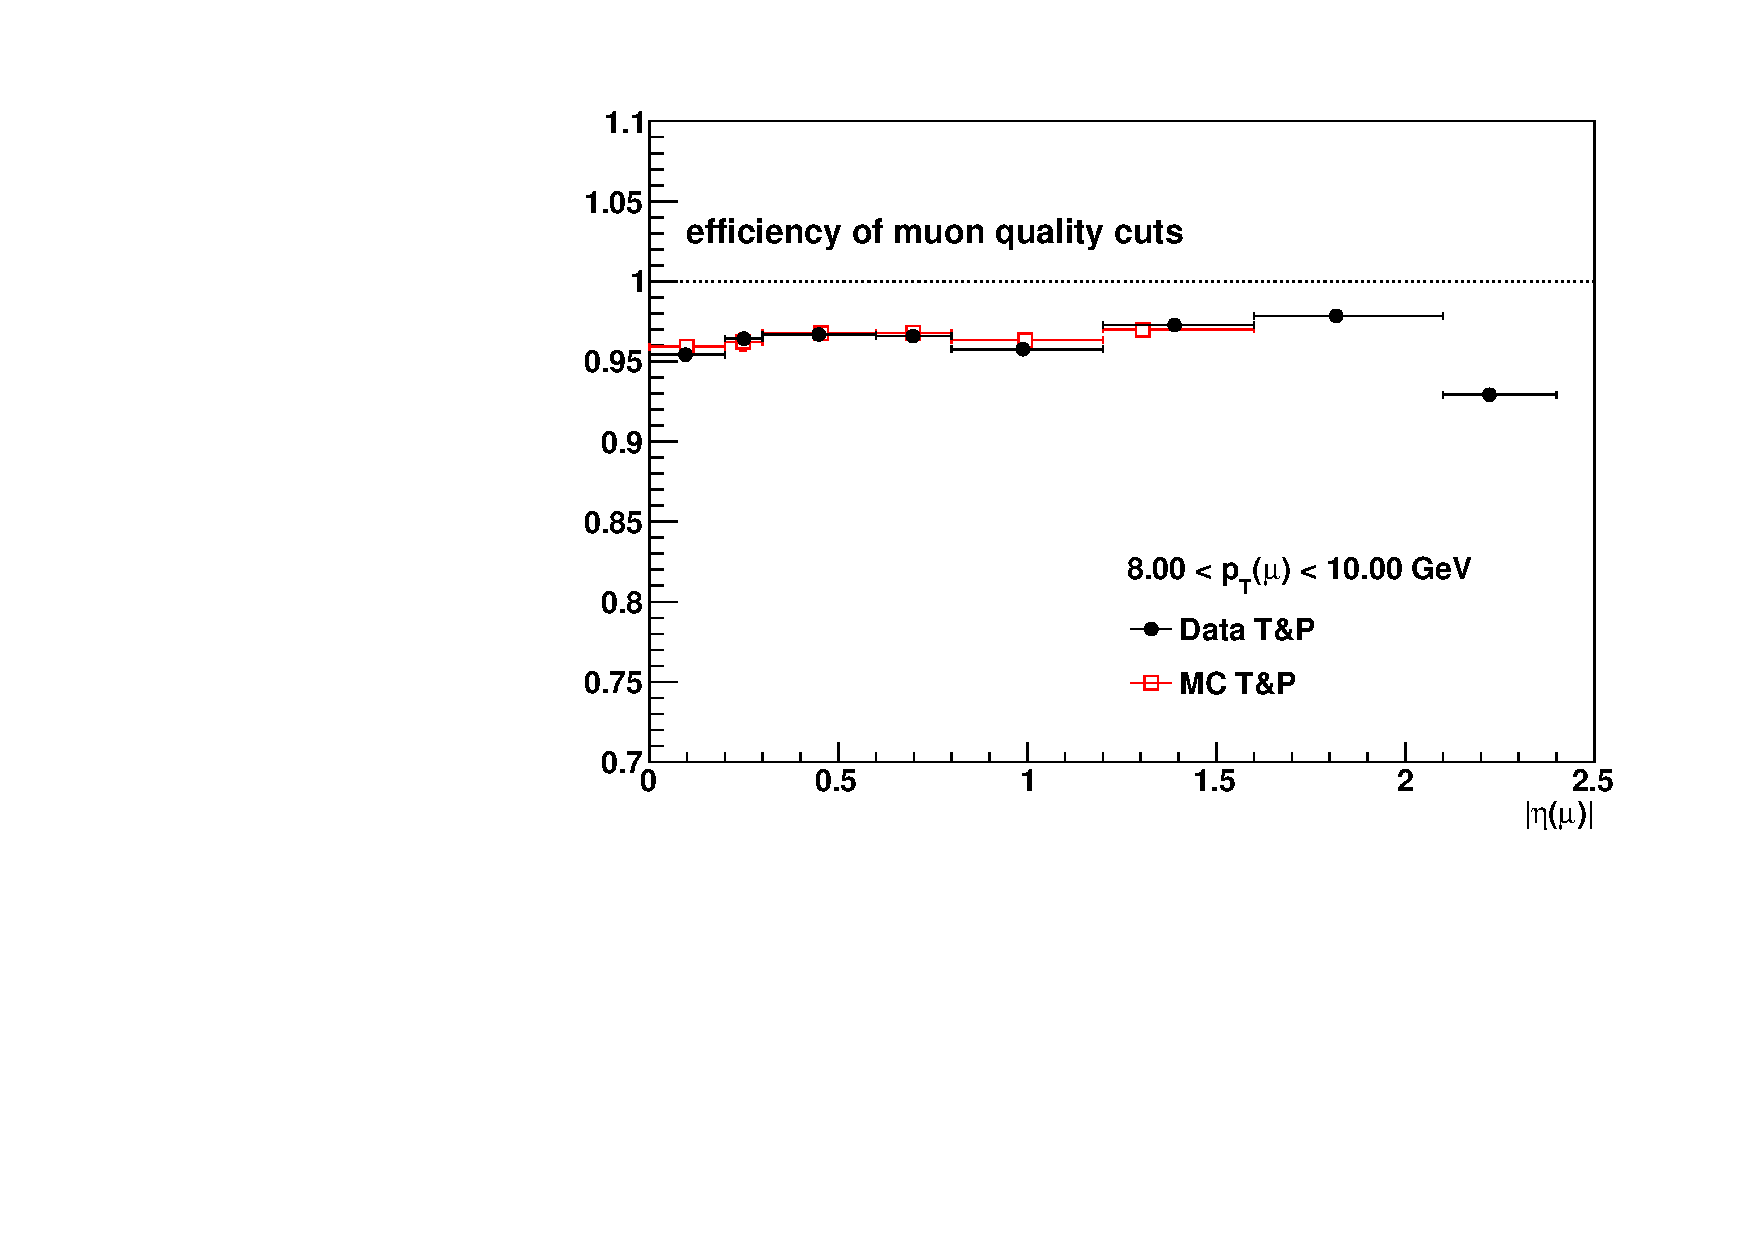
\includegraphics[width=0.49\textwidth]{Figures/\subDirName/MuQualEff_eta_DataVsMC_pTBin10.pdf}
\includegraphics[width=0.49\textwidth]{Figures/\subDirName/MuQualEff_eta_DataVsMC_pTBin11.pdf}
\includegraphics[width=0.49\textwidth]{Figures/\subDirName/MuQualEff_eta_DataVsMC_pTBin12.pdf}
\includegraphics[width=0.49\textwidth]{Figures/\subDirName/MuQualEff_eta_DataVsMC_pTBin13.pdf}
\caption{Continuation of Fig.~\ref{fig:muQualEff-eta-1}.}
\label{fig:muQualEff-eta-2}
\end{figure}

%%%%%%%%%%%%%%%%%%%%%%%%%%%%%%%%%%%%%%
\section{Dimuon trigger inefficiencies for ``close-by'' muons}\label{sec:cowboy}

Given that, at L1, the dimuon triggered samples originally included a
large fraction of ``fake" triggers, caused by coincidental response to
single muons, the CSC L1 trigger group had to implement a ``ghost
busting veto" algorithm which discards dimuon signals, if the two
muons are too close in space. Unfortunately, this cut also rejects
high \pt\ \jpsi's, which can give rise to almost collinear
muons. Furthermore, ``cowboy" dimuons from a \jpsi\ have a high
probability to cross each other at a radius from the interaction point
($R = M / (0.3\cdot B)$) where the muon trigger logic is situated and
are prone to become victims of the ``ghost busting veto" algorithm. The
term ``cowboy" dimuons refers to those pairs that are emitted such
that the magnetic field bends them towards each other, such that their
trajectory can cross (within the muon
detectors), contrary to the so-called ``seagull" dimuons, which are
bent away from each other. The L2 trigger algorithms apply similar
rejection criteria, arbitrating two potential trigger muons that
eventually have survived the L1 trigger veto cut if they share one (or
more) \emph{hits} in common; this currently includes even
\emph{invalid} hits.

In the following we study the inefficiencies induced at L1 and L2
separately, when the two muons are close in space. The L1
trigger efficiency is studied with respect to reconstructed muons,
satisfying the ``BMuQual" criteria and matched to the
\texttt{TrackY} part of the efficiency trigger. Passing probes are
those that have a match to the L1 filter used by all the quarkonium
triggers, ``hltDimuonL1Filtered0". Those reconstructed muons (i.e.\
matched to the L1 filter) become the probes for the ``exclusive" L2
trigger efficiency study, i.e.\ the L2 trigger efficiency with respect
to L1, (L2 $|$ L1). Passing probes for that second step are all those
passing also the L2 filter of the quarkonium triggers,
"hltDimuonL2PreFiltered0".

In Fig.~\ref{fig:CS-comparisonI} we present the L1 and
exclusive L2 trigger efficiencies, separately for cowboy and seagull dimuons.
\begin{figure}[p]
\centering
\includegraphics[width=0.49\textwidth]{Figures/GlobalMuonCuts50/L1L2Eff_SeagullCowboy/L1Eff_abseta_PLOT_pt3_CScomp.pdf}
\includegraphics[width=0.49\textwidth]{Figures/GlobalMuonCuts50/L1L2Eff_SeagullCowboy/L1Eff_pt_PLOT_abseta5_CScomp.pdf}
\includegraphics[width=0.49\textwidth]{Figures/GlobalMuonCuts50/L1L2Eff_SeagullCowboy/L2Eff_abseta_PLOT_pt3_CScomp.pdf}
\includegraphics[width=0.49\textwidth]{Figures/GlobalMuonCuts50/L1L2Eff_SeagullCowboy/L2Eff_pt_PLOT_abseta5_CScomp.pdf}
\includegraphics[width=0.49\textwidth]{Figures/GlobalMuonCuts50/L1L2Eff_SeagullCowboy/L1L2Eff_abseta_PLOT_pt3_CScomp.pdf}
\includegraphics[width=0.49\textwidth]{Figures/GlobalMuonCuts50/L1L2Eff_SeagullCowboy/L1L2Eff_pt_PLOT_abseta5_CScomp.pdf}
\caption{L1 (top) and (L2 $|$ L1) (middle) and L1$\cdot$L2 (bottom)
  trigger efficiencies for ``seagull" and ``cowboy" dimuons, as a
  function of the probe muon's $|\eta|$ (left) and \pt\ (right), for
  the ``global50'' kinematical cuts. }
\label{fig:CS-comparisonI}
\end{figure}

While at mid-rapidity the efficiencies are very similar for
seagull and cowboy dimuons, they become rather different for more
forward rapidities. This can be seen in the left panels, comparing the
red and black points in the two most forward $|\eta|$ bins, as well
as in the right panels, which show the \pt\ dependence for the
forward pseudo-rapidity bin $1.4 < |\eta| < 2.1$.

In Fig.~\ref{fig:CS-comparisonI|} we show the L1 (left) and the
exclusive L2 (right) trigger efficiencies for seagulls and cowboys, in
the pseudo-rapidity range $0.2 < |\eta| < 0.3$.
\begin{figure}[htb]
\centering
\includegraphics[width=0.49\textwidth]{Figures/GlobalMuonCuts50/L1L2Eff_SeagullCowboy/L1Eff_pt_PLOT_abseta1_CScomp.pdf}
\includegraphics[width=0.49\textwidth]{Figures/GlobalMuonCuts50/L1L2Eff_SeagullCowboy/L2Eff_pt_PLOT_abseta1_CScomp.pdf}
\caption{L1 (left) and (L2 $|$ L1) (right) trigger efficiencies for
  ``seagull" and ``cowboy" dimuons, as a function of the probe muon's
  \pt\ for the pseudo-rapidity interval $0.2 < |\eta| < 0.3$, using
  the ``global50'' kinematical cuts.}
\label{fig:CS-comparisonI|}
\end{figure}

This is a problematic region, with a turn-on of the L1 trigger
efficiency less steep than in other $|\Delta\eta|$ regions, given
that the muons cross the uninstrumented gap between the central and
$\pm 1$ muon wheels. On top of that, it seems that there is a rather
significant L1 trigger inefficiency for cowboy dimuons, which is not
seen in the case of the exclusive L2 trigger efficiency.

In the following, we will investigate how these inefficiencies can be
best characterized. For this we consider the single muon \tnp\ trigger
efficiencies as a function of the separation between the tag and the
probe muons, extrapolated to the 2nd muon station. We start by
considering the separation expressed as $\Delta R = \sqrt{\Delta \eta
  ^2 + \Delta \phi ^2}$. The corresponding efficiencies, shown for
cowboy and seagull dimuons, are studied separately when the probe
 \pt\ is smaller or larger than 6~GeV/$c$ and depending on whether
the probe muon is measured at mid- or forward rapidities. The
corresponding study is depicted in Fig.~\ref{fig:deltaR-L1} in the
case of the L1 trigger efficiencies and in Fig.~\ref{fig:deltaR-L2}
for the exclusive L2 trigger efficiencies. In both cases we show the
data driven efficiencies as well as those from our MC simulations.

\begin{figure}[p]
\centering
\includegraphics[width=0.49\textwidth]{Figures/TrackerMuonCuts50/L1L2Eff_SeagullCowboy/L1_deltaRM2_PLOT_abseta0_pt0_CS.pdf}
\includegraphics[width=0.49\textwidth]{Figures/TrackerMuonCuts50/L1L2Eff_SeagullCowboy/L1_deltaRM2_PLOT_abseta0_pt1_CS.pdf}
\includegraphics[width=0.49\textwidth]{Figures/TrackerMuonCuts50/L1L2Eff_SeagullCowboy/L1_deltaRM2_PLOT_abseta1_pt0_CS.pdf}
\includegraphics[width=0.49\textwidth]{Figures/TrackerMuonCuts50/L1L2Eff_SeagullCowboy/L1_deltaRM2_PLOT_abseta1_pt1_CS.pdf}
\includegraphics[width=0.49\textwidth]{Figures/TrackerMuonCuts50/L1L2Eff_SeagullCowboy/L1_deltaRM2_PLOT_abseta2_pt0_CS.pdf}
\includegraphics[width=0.49\textwidth]{Figures/TrackerMuonCuts50/L1L2Eff_SeagullCowboy/L1_deltaRM2_PLOT_abseta2_pt1_CS.pdf}
\includegraphics[width=0.49\textwidth]{Figures/TrackerMuonCuts50/L1L2Eff_SeagullCowboy/L1_deltaRM2_PLOT_abseta3_pt0_CS.pdf}
\includegraphics[width=0.49\textwidth]{Figures/TrackerMuonCuts50/L1L2Eff_SeagullCowboy/L1_deltaRM2_PLOT_abseta3_pt1_CS.pdf}
\caption{L1 trigger efficiency as a function of $\Delta R$,
  extrapolated to the 2nd muon station. Left: for $p_{\rm T} <
  6$~GeV/$c$, Right: for $p_{\rm T} > 6$~GeV/$c$. The rows from top to
  bottom depict calculations in different muon pseudo-rapidity ranges,
  from mid-rapidity (top) to forward rapidity (bottom), using the
  ``tracker50'' muon selection cuts.}
\label{fig:deltaR-L1}
\end{figure}

\begin{figure}[p]
\centering
%\includegraphics[width=0.49\textwidth]{Figures/GlobalMuonCuts50/L1L2Eff_SeagullCowboy/L2_deltaRM2_PLOT_abseta0_pt0_CS.pdf}
%\includegraphics[width=0.49\textwidth]{Figures/GlobalMuonCuts50/L1L2Eff_SeagullCowboy/L2_deltaRM2_PLOT_abseta0_pt1_CS.pdf}
%\includegraphics[width=0.49\textwidth]{Figures/GlobalMuonCuts50/L1L2Eff_SeagullCowboy/L2_deltaRM2_PLOT_abseta1_pt0_CS.pdf}
%\includegraphics[width=0.49\textwidth]{Figures/GlobalMuonCuts50/L1L2Eff_SeagullCowboy/L2_deltaRM2_PLOT_abseta1_pt1_CS.pdf}
%\includegraphics[width=0.49\textwidth]{Figures/GlobalMuonCuts50/L1L2Eff_SeagullCowboy/L2_deltaRM2_PLOT_abseta2_pt0_CS.pdf}
%\includegraphics[width=0.49\textwidth]{Figures/GlobalMuonCuts50/L1L2Eff_SeagullCowboy/L2_deltaRM2_PLOT_abseta2_pt1_CS.pdf}
%\includegraphics[width=0.49\textwidth]{Figures/GlobalMuonCuts50/L1L2Eff_SeagullCowboy/L2_deltaRM2_PLOT_abseta3_pt0_CS.pdf}
%\includegraphics[width=0.49\textwidth]{Figures/GlobalMuonCuts50/L1L2Eff_SeagullCowboy/L2_deltaRM2_PLOT_abseta3_pt1_CS.pdf}
\includegraphics[width=0.49\textwidth]{Figures/GlobalMuonCuts50/L1L2Eff_SeagullCowboy/L2Dimuon0Jpsi_deltaRM2_abseta0_pt0_looseCuts_12Oct2011.pdf}
\includegraphics[width=0.49\textwidth]{Figures/GlobalMuonCuts50/L1L2Eff_SeagullCowboy/L2Dimuon0Jpsi_deltaRM2_abseta0_pt1_looseCuts_12Oct2011.pdf}
\includegraphics[width=0.49\textwidth]{Figures/GlobalMuonCuts50/L1L2Eff_SeagullCowboy/L2Dimuon0Jpsi_deltaRM2_abseta1_pt0_looseCuts_12Oct2011.pdf}
\includegraphics[width=0.49\textwidth]{Figures/GlobalMuonCuts50/L1L2Eff_SeagullCowboy/L2Dimuon0Jpsi_deltaRM2_abseta1_pt1_looseCuts_12Oct2011.pdf}
\includegraphics[width=0.49\textwidth]{Figures/GlobalMuonCuts50/L1L2Eff_SeagullCowboy/L2Dimuon0Jpsi_deltaRM2_abseta2_pt0_looseCuts_12Oct2011.pdf}
\includegraphics[width=0.49\textwidth]{Figures/GlobalMuonCuts50/L1L2Eff_SeagullCowboy/L2Dimuon0Jpsi_deltaRM2_abseta2_pt1_looseCuts_12Oct2011.pdf}
\includegraphics[width=0.49\textwidth]{Figures/GlobalMuonCuts50/L1L2Eff_SeagullCowboy/L2Dimuon0Jpsi_deltaRM2_abseta3_pt0_looseCuts_12Oct2011.pdf}
\includegraphics[width=0.49\textwidth]{Figures/GlobalMuonCuts50/L1L2Eff_SeagullCowboy/L2Dimuon0Jpsi_deltaRM2_abseta3_pt1_looseCuts_12Oct2011.pdf}
\caption{same as Fig.~\ref{fig:deltaR-L1}, except for the exclusive L2
  trigger efficiency, (L2 $|$ L1) and using the ``global50'' kinematical cuts.}
\label{fig:deltaR-L2}
\end{figure}

While the efficiencies for cowboy and seagull dimuons are rather
similar for $|\eta| < 1.2$, not showing a strong $\Delta R$
dependence, we see an inefficiency developing for cowboy dimuons with
close separation, when $|\eta| > 1.2$. Interestingly, these
inefficiencies are more pronounced for the exclusive L2 trigger
efficiency: while the bin $1.2 < |\eta| < 1.6$ and $p_{\rm T} <
6$~GeV/$c$ does not present an inefficiency for cowboy dimuons, at L1,
they experience an inefficiency of up to 50\,\% at L2. This
inefficiency becomes rather pronounced for $1.6 < |\eta| < 2.1$ with
inefficiencies, starting for $\Delta R < 0.5$. The fact that the
trigger efficiencies decrease for large $\Delta R$ separations is
probably due to a hidden \pt\ dependence: large $\Delta R$, i.e.\
large opening between the two muons, is characteristic of low \pt\
\jpsi's which have an overall lower trigger efficiency (as will be
shown in Section~\ref{sec:eps_L1L2}). Given that the figures are
integrated over the range $p_{\rm T} < 6$~GeV/$c$, which represents
the full dynamic range (only true if cut on single muon
efficiencies!!!  check!) in which the efficiencies rise from 0 to
almost 100\,\% events with large $\Delta R$ separation are most likely
integrated over a significantly lower \pt\ range.

To separate the individual components of the $\Delta R$ dependences, the
study was repeated as a function of $\Delta \phi$, also evaluated at
the second muon station. The corresponding results are depicted in
Figs.~\ref{fig:deltaPhi-L1} and \ref{fig:deltaPhi-L2}.
\begin{figure}[p]
\centering
\includegraphics[width=0.49\textwidth]{Figures/TrackerMuonCuts50/L1L2Eff_SeagullCowboy/L1_deltaPhiM2_PLOT_abseta0_pt0_CS.pdf}
\includegraphics[width=0.49\textwidth]{Figures/TrackerMuonCuts50/L1L2Eff_SeagullCowboy/L1_deltaPhiM2_PLOT_abseta0_pt1_CS.pdf}
\includegraphics[width=0.49\textwidth]{Figures/TrackerMuonCuts50/L1L2Eff_SeagullCowboy/L1_deltaPhiM2_PLOT_abseta1_pt0_CS.pdf}
\includegraphics[width=0.49\textwidth]{Figures/TrackerMuonCuts50/L1L2Eff_SeagullCowboy/L1_deltaPhiM2_PLOT_abseta1_pt1_CS.pdf}
\includegraphics[width=0.49\textwidth]{Figures/TrackerMuonCuts50/L1L2Eff_SeagullCowboy/L1_deltaPhiM2_PLOT_abseta2_pt0_CS.pdf}
\includegraphics[width=0.49\textwidth]{Figures/TrackerMuonCuts50/L1L2Eff_SeagullCowboy/L1_deltaPhiM2_PLOT_abseta2_pt1_CS.pdf}
\includegraphics[width=0.49\textwidth]{Figures/TrackerMuonCuts50/L1L2Eff_SeagullCowboy/L1_deltaPhiM2_PLOT_abseta3_pt0_CS.pdf}
\includegraphics[width=0.48\textwidth]{Figures/TrackerMuonCuts50/L1L2Eff_SeagullCowboy/L1_deltaPhiM2_PLOT_abseta3_pt1_CS.pdf}
\caption{L1 trigger efficiency as a function of $\Delta \phi$,
  extrapolated to the 2nd muon station. Left: for $p_{\rm T} <
  6$~GeV/$c$, Right: for $p_{\rm T} > 6$~GeV/$c$. The rows from top to
  bottom depict calculations in different muon pseudo-rapidity ranges,
  from mid-rapidity (top) to forward rapidity (bottom), using the
  ``tracker50'' kinematical cuts.}
\label{fig:deltaPhi-L1}
\end{figure}

\begin{figure}[p]
\centering
%\includegraphics[width=0.49\textwidth]{Figures/GlobalMuonCuts50/L1L2Eff_SeagullCowboy/L2_deltaPhiM2_PLOT_abseta0_pt0_CS.pdf}
%\includegraphics[width=0.49\textwidth]{Figures/GlobalMuonCuts50/L1L2Eff_SeagullCowboy/L2_deltaPhiM2_PLOT_abseta0_pt1_CS.pdf}
%\includegraphics[width=0.49\textwidth]{Figures/GlobalMuonCuts50/L1L2Eff_SeagullCowboy/L2_deltaPhiM2_PLOT_abseta1_pt0_CS.pdf}
%\includegraphics[width=0.49\textwidth]{Figures/GlobalMuonCuts50/L1L2Eff_SeagullCowboy/L2_deltaPhiM2_PLOT_abseta1_pt1_CS.pdf}
%\includegraphics[width=0.49\textwidth]{Figures/GlobalMuonCuts50/L1L2Eff_SeagullCowboy/L2_deltaPhiM2_PLOT_abseta2_pt0_CS.pdf}
%\includegraphics[width=0.49\textwidth]{Figures/GlobalMuonCuts50/L1L2Eff_SeagullCowboy/L2_deltaPhiM2_PLOT_abseta2_pt1_CS.pdf}
%\includegraphics[width=0.49\textwidth]{Figures/GlobalMuonCuts50/L1L2Eff_SeagullCowboy/L2_deltaPhiM2_PLOT_abseta3_pt0_CS.pdf}
%\includegraphics[width=0.49\textwidth]{Figures/GlobalMuonCuts50/L1L2Eff_SeagullCowboy/L2_deltaPhiM2_PLOT_abseta3_pt1_CS.pdf}
\includegraphics[width=0.49\textwidth]{Figures/GlobalMuonCuts50/L1L2Eff_SeagullCowboy/L2Dimuon0Jpsi_deltaPhiM2_abseta0_pt0_looseCuts_12Oct2011.pdf}
\includegraphics[width=0.49\textwidth]{Figures/GlobalMuonCuts50/L1L2Eff_SeagullCowboy/L2Dimuon0Jpsi_deltaPhiM2_abseta0_pt1_looseCuts_12Oct2011.pdf}
\includegraphics[width=0.49\textwidth]{Figures/GlobalMuonCuts50/L1L2Eff_SeagullCowboy/L2Dimuon0Jpsi_deltaPhiM2_abseta1_pt0_looseCuts_12Oct2011.pdf}
\includegraphics[width=0.49\textwidth]{Figures/GlobalMuonCuts50/L1L2Eff_SeagullCowboy/L2Dimuon0Jpsi_deltaPhiM2_abseta1_pt1_looseCuts_12Oct2011.pdf}
\includegraphics[width=0.49\textwidth]{Figures/GlobalMuonCuts50/L1L2Eff_SeagullCowboy/L2Dimuon0Jpsi_deltaPhiM2_abseta2_pt0_looseCuts_12Oct2011.pdf}
\includegraphics[width=0.49\textwidth]{Figures/GlobalMuonCuts50/L1L2Eff_SeagullCowboy/L2Dimuon0Jpsi_deltaPhiM2_abseta2_pt1_looseCuts_12Oct2011.pdf}
\includegraphics[width=0.49\textwidth]{Figures/GlobalMuonCuts50/L1L2Eff_SeagullCowboy/L2Dimuon0Jpsi_deltaPhiM2_abseta3_pt0_looseCuts_12Oct2011.pdf}
\includegraphics[width=0.49\textwidth]{Figures/GlobalMuonCuts50/L1L2Eff_SeagullCowboy/L2Dimuon0Jpsi_deltaPhiM2_abseta3_pt1_looseCuts_12Oct2011.pdf}
\caption{same as Fig.~\ref{fig:deltaPhi-L1}, except for the exclusive
  L2 trigger efficiency, (L2 $|$ L1) and using the ``global50''
  kinematical cuts.}
\label{fig:deltaPhi-L2}
\end{figure}

At mid-rapidity, also the cowboy dimuons have a natural separation in
$\Delta \phi$ and, hence, do not suffer from inefficiencies. The first
bin in which the range $\Delta\phi < 0.4$ starts being populated is
$1.2 < |\eta| < 1.6$ and an inefficiency develops getting stronger for
small values of $\Delta\phi$ and higher $\eta$. As was observed
before, these inefficiencies are more pronounced for the exclusive L2
trigger efficiencies.

\begin{figure}[p]
\centering
\includegraphics[width=0.49\textwidth]{Figures/TrackerMuonCuts50/L1L2Eff_SeagullCowboy/L1_distM2_PLOT_abseta0_pt0_CS.pdf}
\includegraphics[width=0.49\textwidth]{Figures/TrackerMuonCuts50/L1L2Eff_SeagullCowboy/L1_distM2_PLOT_abseta0_pt1_CS.pdf}
\includegraphics[width=0.49\textwidth]{Figures/TrackerMuonCuts50/L1L2Eff_SeagullCowboy/L1_distM2_PLOT_abseta1_pt0_CS.pdf}
\includegraphics[width=0.49\textwidth]{Figures/TrackerMuonCuts50/L1L2Eff_SeagullCowboy/L1_distM2_PLOT_abseta1_pt1_CS.pdf}
\includegraphics[width=0.49\textwidth]{Figures/TrackerMuonCuts50/L1L2Eff_SeagullCowboy/L1_distM2_PLOT_abseta2_pt0_CS.pdf}
\includegraphics[width=0.49\textwidth]{Figures/TrackerMuonCuts50/L1L2Eff_SeagullCowboy/L1_distM2_PLOT_abseta2_pt1_CS.pdf}
\includegraphics[width=0.49\textwidth]{Figures/TrackerMuonCuts50/L1L2Eff_SeagullCowboy/L1_distM2_PLOT_abseta3_pt0_CS.pdf}
\includegraphics[width=0.48\textwidth]{Figures/TrackerMuonCuts50/L1L2Eff_SeagullCowboy/L1_distM2_PLOT_abseta3_pt1_CS.pdf}
\caption{L1 trigger efficiency as a function of the distance between
  the two muons, measured in the 2nd muon station. Left: for $p_{\rm
    T} < 6$~GeV/$c$, Right: for $p_{\rm T} > 6$~GeV/$c$. The rows from
  top to bottom depict calculations in different muon pseudo-rapidity
  ranges, from mid-rapidity (top) to forward rapidity (bottom), using
  the ``tracker50'' kinematical cuts.}
\label{fig:distM2-L1}
\end{figure}

\begin{figure}[p]
\centering
%\includegraphics[width=0.49\textwidth]{Figures/GlobalMuonCuts50/L1L2Eff_SeagullCowboy/L2_distM2_PLOT_abseta0_pt0_CS.pdf}
%\includegraphics[width=0.49\textwidth]{Figures/GlobalMuonCuts50/L1L2Eff_SeagullCowboy/L2_distM2_PLOT_abseta0_pt1_CS.pdf}
%\includegraphics[width=0.49\textwidth]{Figures/GlobalMuonCuts50/L1L2Eff_SeagullCowboy/L2_distM2_PLOT_abseta1_pt0_CS.pdf}
%\includegraphics[width=0.49\textwidth]{Figures/GlobalMuonCuts50/L1L2Eff_SeagullCowboy/L2_distM2_PLOT_abseta1_pt1_CS.pdf}
%\includegraphics[width=0.49\textwidth]{Figures/GlobalMuonCuts50/L1L2Eff_SeagullCowboy/L2_distM2_PLOT_abseta2_pt0_CS.pdf}
%\includegraphics[width=0.49\textwidth]{Figures/GlobalMuonCuts50/L1L2Eff_SeagullCowboy/L2_distM2_PLOT_abseta2_pt1_CS.pdf}
%\includegraphics[width=0.49\textwidth]{Figures/GlobalMuonCuts50/L1L2Eff_SeagullCowboy/L2_distM2_PLOT_abseta3_pt0_CS.pdf}
%\includegraphics[width=0.49\textwidth]{Figures/GlobalMuonCuts50/L1L2Eff_SeagullCowboy/L2_distM2_PLOT_abseta3_pt1_CS.pdf}
\includegraphics[width=0.49\textwidth]{Figures/TrackerMuonCuts50/L1L2Eff_SeagullCowboy/L2Dimuon0Jpsi_distM2_abseta0_pt0_looseCuts_12Oct2011.pdf}
\includegraphics[width=0.49\textwidth]{Figures/TrackerMuonCuts50/L1L2Eff_SeagullCowboy/L2Dimuon0Jpsi_distM2_abseta0_pt1_looseCuts_12Oct2011.pdf}
\includegraphics[width=0.49\textwidth]{Figures/TrackerMuonCuts50/L1L2Eff_SeagullCowboy/L2Dimuon0Jpsi_distM2_abseta1_pt0_looseCuts_12Oct2011.pdf}
\includegraphics[width=0.49\textwidth]{Figures/TrackerMuonCuts50/L1L2Eff_SeagullCowboy/L2Dimuon0Jpsi_distM2_abseta1_pt1_looseCuts_12Oct2011.pdf}
\includegraphics[width=0.49\textwidth]{Figures/TrackerMuonCuts50/L1L2Eff_SeagullCowboy/L2Dimuon0Jpsi_distM2_abseta2_pt0_looseCuts_12Oct2011.pdf}
\includegraphics[width=0.49\textwidth]{Figures/TrackerMuonCuts50/L1L2Eff_SeagullCowboy/L2Dimuon0Jpsi_distM2_abseta2_pt1_looseCuts_12Oct2011.pdf}
\includegraphics[width=0.49\textwidth]{Figures/TrackerMuonCuts50/L1L2Eff_SeagullCowboy/L2Dimuon0Jpsi_distM2_abseta3_pt0_looseCuts_12Oct2011.pdf}
\includegraphics[width=0.49\textwidth]{Figures/TrackerMuonCuts50/L1L2Eff_SeagullCowboy/L2Dimuon0Jpsi_distM2_abseta3_pt1_looseCuts_12Oct2011.pdf}
\caption{same as Fig.~\ref{fig:distM2-L1}, except for the exclusive L2
  trigger efficiency, (L2 $|$ L1).}
\label{fig:distM2-L2}
\end{figure}

We have equally studied the cowboy inefficiencies versus the physical
distance between the two muons, in meters, measured at the 2nd muon
station. The corresponding results are shown in
Figs.~\ref{fig:distM2-L1} and \ref{fig:distM2-L2}. Even though they
qualitatively do not add any further information (same inefficiencies
as in the previous figures) it is striking to realize that the
observed inefficiencies are visible up to a separation of around
150~cm.

%%%%%%%%%%%%%%%%%%%%%%%%%%%%%%%%%%%%%%%%%%%%%%%%%%
\section{L1$\cdot$L2 trigger efficiency}\label{sec:eps_L1L2}

Discarding cowboy dimuons from the further studies\footnote{for
  completeness the trigger efficiencies for cowboy dimuons are given
  in Appendix C}, we investigate the
L1$\cdot$L2 trigger efficiencies with respect to reconstructed muons,
satisfying the quality criteria (``BMuQual'') outlined in
Section~\ref{sec:muQual}. Besides, we match the probe to the
\texttt{TrackY} part of efficiency trigger object. Passing probes are
those matched to the L2 filter "hltDimuonL2PreFiltered0". Given that
this L2 filter is used by all the dimuon triggers in the MuOnia PD,
most of which are unprescaled, no prescale factors need to be taken
into account. It should be noted that, even though the MuX\_TrackY
trigger is a ``single'' muon trigger and has different L1 requirements
(different L1 quality bit), with respect to the physics trigger under
study there is no bias in the extraction of the corresponding L1 (and
L2) trigger efficiencies: the quality criteria imposed on single
muon triggers are, in general, \emph{stricter} than for double muon
triggers. If the pair is inefficient in a given event, it is not
because of the tag possibly being inefficient, given that a matching
is requested to a dimuon trigger filter.

The resulting efficiencies, for the L1\_DoubleMu0
seed (used during the run period $165088-173236$) can be seen in \pt\
differential form in Fig.~\ref{fig:L1L2Eff-pt} and in $|\eta|$
differential form in Figs.~\ref{fig:L1L2Eff-eta-1} and \ref{fig:L1L2Eff-eta-2}.

\begin{figure}[p]
\centering
\includegraphics[width=0.49\textwidth]{Figures/\subDirName/L1L2-run1/L1L2Eff_pT_DataVsMC_etaBin0.pdf}
\includegraphics[width=0.49\textwidth]{Figures/\subDirName/L1L2-run1/L1L2Eff_pT_DataVsMC_etaBin1.pdf}
\includegraphics[width=0.49\textwidth]{Figures/\subDirName/L1L2-run1/L1L2Eff_pT_DataVsMC_etaBin2.pdf}
\includegraphics[width=0.49\textwidth]{Figures/\subDirName/L1L2-run1/L1L2Eff_pT_DataVsMC_etaBin3.pdf}
\includegraphics[width=0.49\textwidth]{Figures/\subDirName/L1L2-run1/L1L2Eff_pT_DataVsMC_etaBin4.pdf}
\includegraphics[width=0.49\textwidth]{Figures/\subDirName/L1L2-run1/L1L2Eff_pT_DataVsMC_etaBin5.pdf}
%only for Tracker muon cuts
\includegraphics[width=0.49\textwidth]{Figures/\subDirName/L1L2-run1/L1L2Eff_pT_DataVsMC_etaBin6.pdf}
%only for Tracker muon cuts
\includegraphics[width=0.49\textwidth]{Figures/\subDirName/L1L2-run1/L1L2Eff_pT_DataVsMC_etaBin7.pdf}
\caption{L1$\cdot$L2 trigger efficiency, using the L1\_DoubleMu0 seed,
  versus \pt\ in various slices in $|\eta|$, using the ``tracker50'' muon
  cuts ($165088 - 172868$).}
\label{fig:L1L2Eff-pt}
\end{figure}
\begin{figure}[p]
\centering
\includegraphics[width=0.49\textwidth]{Figures/\subDirName/L1L2-run1/L1L2Eff_eta_DataVsMC_pTBin0.pdf}
\includegraphics[width=0.49\textwidth]{Figures/\subDirName/L1L2-run1/L1L2Eff_eta_DataVsMC_pTBin1.pdf}
\includegraphics[width=0.49\textwidth]{Figures/\subDirName/L1L2-run1/L1L2Eff_eta_DataVsMC_pTBin2.pdf}
\includegraphics[width=0.49\textwidth]{Figures/\subDirName/L1L2-run1/L1L2Eff_eta_DataVsMC_pTBin3.pdf}
\includegraphics[width=0.49\textwidth]{Figures/\subDirName/L1L2-run1/L1L2Eff_eta_DataVsMC_pTBin4.pdf}
\includegraphics[width=0.49\textwidth]{Figures/\subDirName/L1L2-run1/L1L2Eff_eta_DataVsMC_pTBin5.pdf}
\includegraphics[width=0.49\textwidth]{Figures/\subDirName/L1L2-run1/L1L2Eff_eta_DataVsMC_pTBin6.pdf}
\includegraphics[width=0.49\textwidth]{Figures/\subDirName/L1L2-run1/L1L2Eff_eta_DataVsMC_pTBin7.pdf}
\caption{L1$\cdot$L2 trigger efficiency, using the L1\_DoubleMu0 seed,
  versus $|\eta|$ for small slices in \pt, using the ``tracker50'' muon
  cuts ($165088 - 172868$).}
\label{fig:L1L2Eff-eta-1}
\end{figure}
\begin{figure}[p]
\centering
\includegraphics[width=0.49\textwidth]{Figures/\subDirName/L1L2-run1/L1L2Eff_eta_DataVsMC_pTBin8.pdf}
\includegraphics[width=0.49\textwidth]{Figures/\subDirName/L1L2-run1/L1L2Eff_eta_DataVsMC_pTBin9.pdf}
\includegraphics[width=0.49\textwidth]{Figures/\subDirName/L1L2-run1/L1L2Eff_eta_DataVsMC_pTBin10.pdf}
\includegraphics[width=0.49\textwidth]{Figures/\subDirName/L1L2-run1/L1L2Eff_eta_DataVsMC_pTBin11.pdf}
\includegraphics[width=0.49\textwidth]{Figures/\subDirName/L1L2-run1/L1L2Eff_eta_DataVsMC_pTBin12.pdf}
\includegraphics[width=0.49\textwidth]{Figures/\subDirName/L1L2-run1/L1L2Eff_eta_DataVsMC_pTBin13.pdf}
\caption{Continuation of Fig.~\ref{fig:L1L2Eff-eta-1}.}
\label{fig:L1L2Eff-eta-2}
\end{figure}

Also here, the data have sufficient statistical accuracy, such that a
clear trend is visible, showing the expected \pt\ turn-on behaviour in
each of the $|\eta|$ slices. The rise of the turn-on curve is
sufficiently steep such that the plateau value is reached below
10~GeV/$c$. The bin $0.2 < |\eta| < 0.3$ is affected by stronger
inefficiencies because muons passing through the non-instrumented
region between the central and $\pm 1$ wheels fail to fire the
trigger. 

The MC based \tnp\ efficiencies reproduce well the overall trend, in
practically all $|\eta|$ slices. The values are not identical,
partially because the centre of gravity of a given bin is slightly
different in data and MC, given that the generation was performed flat in
\pt.
% The only exception is the last \pt\
%value of the bin $0.2 < |\eta| < 0.3$: while the data point indicates
%a value of $9x\pm xxx$ (Ilse???), the MC equivalent show $9x \pm xxx$
%(Ilse ???), significantly different. Do we know why ???

The above study was performed for the run range in which the
L1\_DoubleMu0 trigger seed was used. From the 3E33 trigger menu
onwards (starting from run 173236), the L1\_DoubleMu0\_HighQ seed was
used instead, given that signal efficiency was expected to be very
similar, while significnatly reducing the trigger rate. The changes
concern certain classes of unconfirmed CSC
candidates~\cite{IvanTWiki}, such that we only expect differences for
$|\eta| > 1.2$.

Fig.~\ref{fig:L1L2Eff-HighQ-MC} shows the comparison of
L1$\cdot$L2 trigger efficiencies for data (left) and MC (right) for
the two different L1 trigger seeds.  The data are affected by
significant statistical fluctuations, such that a data comparison in
the two run ranges is not very meaningful.  Efficiency triggers are
heavily prescaled in the L1\_DoubleMu0\_HighQ period, even if most of
the physics triggers are collected in that period.
\begin{figure}[htb]
\centering
%\includegraphics[width=0.49\textwidth]{Figures/TrackerMuonCuts50/L1L2Dimuon0Jpsi_gEff_DATA_PT_AETA5_run1vs2_data_25Oct2011.pdf}
%\includegraphics[width=0.49\textwidth]{Figures/TrackerMuonCuts50/L1L2Dimuon0Jpsi_gEff_MC_PT_AETA5_run1vs2_MC_25Oct2011.pdf}
\includegraphics[width=0.49\textwidth]{Figures/TrackerMuonCuts50_FineBins/L1L2Dimuon0Jpsi_gEff_DATA_PT_AETA5_run1vs2_data_15Nov2011.pdf}
\includegraphics[width=0.49\textwidth]{Figures/TrackerMuonCuts50_FineBins/L1L2Dimuon0Jpsi_gEff_MC_PT_AETA5_run1vs2_MC_15Nov2011.pdf}
\caption{Comparison of the L1$\cdot$L2 trigger efficiency with the
  L1\_DoubleMu0 and L1\_DoubleMu0\_HighQ trigger seeds, using the
  ``tracker50'' muon cuts. Left: data, Right:
MC.}
\label{fig:L1L2Eff-HighQ-MC}
\end{figure}

The corresponding comparisons in MC show a noticably lower
L1$\cdot$L2 trigger efficiency with the L1\_DoubleMu0\_HighQ seed, which
becomes more pronounced at low \pt.

As anticipated in Section~\ref{sec:dataSets} the GMT changed settings in
run 175971 which was then kept until the end of data taking. We have
also studied the L1$\cdot$L2 trigger efficiencies during that run
period and compared it to the first period of data taking. These
comparisons can be seen in Fig.~\ref{fig:L1L2Eff-run13-pt} and
\ref{fig:L1L2Eff-run13-eta}. 
\begin{figure}[p]
\centering
\includegraphics[width=0.49\textwidth]{Figures/TrackerMuonCuts50/L1L2-run3/L1L2Dimuon0Jpsi_gEff_DATA_PT_AETA0_runComp13_TrkCuts_9Nov2011.pdf}
\includegraphics[width=0.49\textwidth]{Figures/TrackerMuonCuts50/L1L2-run3/L1L2Dimuon0Jpsi_gEff_DATA_PT_AETA1_runComp13_TrkCuts_9Nov2011.pdf}
\includegraphics[width=0.49\textwidth]{Figures/TrackerMuonCuts50/L1L2-run3/L1L2Dimuon0Jpsi_gEff_DATA_PT_AETA2_runComp13_TrkCuts_9Nov2011.pdf}
\includegraphics[width=0.49\textwidth]{Figures/TrackerMuonCuts50/L1L2-run3/L1L2Dimuon0Jpsi_gEff_DATA_PT_AETA3_runComp13_TrkCuts_9Nov2011.pdf}
\includegraphics[width=0.49\textwidth]{Figures/TrackerMuonCuts50/L1L2-run3/L1L2Dimuon0Jpsi_gEff_DATA_PT_AETA4_runComp13_TrkCuts_9Nov2011.pdf}
\includegraphics[width=0.49\textwidth]{Figures/TrackerMuonCuts50/L1L2-run3/L1L2Dimuon0Jpsi_gEff_DATA_PT_AETA5_runComp13_TrkCuts_9Nov2011.pdf}
\includegraphics[width=0.49\textwidth]{Figures/TrackerMuonCuts50/L1L2-run3/L1L2Dimuon0Jpsi_gEff_DATA_PT_AETA6_runComp13_TrkCuts_9Nov2011.pdf}
\includegraphics[width=0.49\textwidth]{Figures/TrackerMuonCuts50/L1L2-run3/L1L2Dimuon0Jpsi_gEff_DATA_PT_AETA7_runComp13_TrkCuts_9Nov2011.pdf}
\caption{Comparison of the L1$\cdot$L2 trigger efficiency during two
  different run periods, versus \pt\ for small slices in $|\eta|$,
  using the ``tracker50'' muon cuts.}
\label{fig:L1L2Eff-run13-pt}
\end{figure}
\begin{figure}[p]
\centering
\includegraphics[width=0.49\textwidth]{Figures/TrackerMuonCuts50/L1L2-run3/L1L2Dimuon0Jpsi_gEff_DATA_AETA_PT0_runComp13_TrkCuts_9Nov2011.pdf}
\includegraphics[width=0.49\textwidth]{Figures/TrackerMuonCuts50/L1L2-run3/L1L2Dimuon0Jpsi_gEff_DATA_AETA_PT1_runComp13_TrkCuts_9Nov2011.pdf}
\includegraphics[width=0.49\textwidth]{Figures/TrackerMuonCuts50/L1L2-run3/L1L2Dimuon0Jpsi_gEff_DATA_AETA_PT2_runComp13_TrkCuts_9Nov2011.pdf}
\includegraphics[width=0.49\textwidth]{Figures/TrackerMuonCuts50/L1L2-run3/L1L2Dimuon0Jpsi_gEff_DATA_AETA_PT3_runComp13_TrkCuts_9Nov2011.pdf}
\includegraphics[width=0.49\textwidth]{Figures/TrackerMuonCuts50/L1L2-run3/L1L2Dimuon0Jpsi_gEff_DATA_AETA_PT4_runComp13_TrkCuts_9Nov2011.pdf}
\includegraphics[width=0.49\textwidth]{Figures/TrackerMuonCuts50/L1L2-run3/L1L2Dimuon0Jpsi_gEff_DATA_AETA_PT5_runComp13_TrkCuts_9Nov2011.pdf}
\includegraphics[width=0.49\textwidth]{Figures/TrackerMuonCuts50/L1L2-run3/L1L2Dimuon0Jpsi_gEff_DATA_AETA_PT6_runComp13_TrkCuts_9Nov2011.pdf}
\includegraphics[width=0.49\textwidth]{Figures/TrackerMuonCuts50/L1L2-run3/L1L2Dimuon0Jpsi_gEff_DATA_AETA_PT7_runComp13_TrkCuts_9Nov2011.pdf}
\caption{Comparison of the L1$\cdot$L2 trigger efficiency during two
  different run periods, versus $|\eta|$ for small slices in \pt,
  using the ``tracker50'' muon cuts.}
\label{fig:L1L2Eff-run13-eta}
\end{figure}

There seems to be a small efficiency drop which is readily seen from
the $|\eta|$ dependent efficiencies. 
%%%%%%%%%%%%%%%%%%%%%%%%%%%%%%%%%%%%%%%%%%%%%%%%%%
\section{L3 trigger efficiency}\label{sec:eps_L3}

The L3 trigger efficiencies presented here are not those specific to a
certain L3 trigger filter, but correspond to the intrinsic trigger
efficiencies of L3 muons. In other words, the efficiencies shown here
do not account for cuts used in specific L3 filters. This is motivated
by the fact that, in this way, the full \pt\ and $\eta$ ranges of L3
muons can be measured; the effects of other cuts, like the DCA cut
(distance of closest approach between the two muons), which is part of
practically all L3 muon filters in the MuOnia PD, need to be evaluated
in an independent way. Moreover, with the standard \tnp\ skim for
efficiency studies of a given probe, as opposed to studies of the
\emph{pair}, the effect of this specific cut cannot be
evaluated.

In concrete terms, the tag muon is matched (as usual) to the HLT muon
in the trigger path HLT\_Mu5\_L2Mu2\_Jpsi and the probe muon must pass
the corresponding L2 filter \\
(``hltMu5L2Mu2JpsiTrackMassFiltered'') and the ``BMuQual'' quality
criteria.  Passing probes are then identified as those that are
contained in the collection \texttt{hltL3MuonCandidates}. The \pt\
($|\eta|$) differential efficiencies, studied for seagull dimuons
only\footnote{for completeness the trigger efficiencies for cowboy
  dimuons are given in Appendix C.}, can be found in
Fig.~\ref{fig:L3Eff-pt} (\ref{fig:L3Eff-eta-1} and \ref{fig:L3Eff-eta-2}).

\begin{figure}[p]
\centering
\includegraphics[width=0.49\textwidth]{Figures/\subDirName/L3-run1/L3Eff_pT_DataVsMC_etaBin0.pdf}
\includegraphics[width=0.49\textwidth]{Figures/\subDirName/L3-run1/L3Eff_pT_DataVsMC_etaBin1.pdf}
\includegraphics[width=0.49\textwidth]{Figures/\subDirName/L3-run1/L3Eff_pT_DataVsMC_etaBin2.pdf}
\includegraphics[width=0.49\textwidth]{Figures/\subDirName/L3-run1/L3Eff_pT_DataVsMC_etaBin3.pdf}
\includegraphics[width=0.49\textwidth]{Figures/\subDirName/L3-run1/L3Eff_pT_DataVsMC_etaBin4.pdf}
\includegraphics[width=0.49\textwidth]{Figures/\subDirName/L3-run1/L3Eff_pT_DataVsMC_etaBin5.pdf}
\includegraphics[width=0.49\textwidth]{Figures/\subDirName/L3-run1/L3Eff_pT_DataVsMC_etaBin6.pdf}
\includegraphics[width=0.49\textwidth]{Figures/\subDirName/L3-run1/L3Eff_pT_DataVsMC_etaBin7.pdf}
\caption{L3 trigger efficiency versus \pt\ in various slices in
  $|\eta|$, using the ``tracker50'' muon cuts ($165088 - 178379$).}
\label{fig:L3Eff-pt}
\end{figure}
\begin{figure}[p]
\centering
\includegraphics[width=0.49\textwidth]{Figures/\subDirName/L3-run1/L3Eff_eta_DataVsMC_pTBin0.pdf}
\includegraphics[width=0.49\textwidth]{Figures/\subDirName/L3-run1/L3Eff_eta_DataVsMC_pTBin1.pdf}
\includegraphics[width=0.49\textwidth]{Figures/\subDirName/L3-run1/L3Eff_eta_DataVsMC_pTBin2.pdf}
\includegraphics[width=0.49\textwidth]{Figures/\subDirName/L3-run1/L3Eff_eta_DataVsMC_pTBin3.pdf}
\includegraphics[width=0.49\textwidth]{Figures/\subDirName/L3-run1/L3Eff_eta_DataVsMC_pTBin4.pdf}
\includegraphics[width=0.49\textwidth]{Figures/\subDirName/L3-run1/L3Eff_eta_DataVsMC_pTBin5.pdf}
\includegraphics[width=0.49\textwidth]{Figures/\subDirName/L3-run1/L3Eff_eta_DataVsMC_pTBin6.pdf}
\includegraphics[width=0.49\textwidth]{Figures/\subDirName/L3-run1/L3Eff_eta_DataVsMC_pTBin7.pdf}
\caption{L3 trigger efficiency versus $|\eta|$ for small slices in
  \pt, using the ``tracker50'' muon cuts ($165088 - 178379$).}
\label{fig:L3Eff-eta-1}
\end{figure}
\begin{figure}[p]
\centering
\includegraphics[width=0.49\textwidth]{Figures/\subDirName/L3-run1/L3Eff_eta_DataVsMC_pTBin8.pdf}
\includegraphics[width=0.49\textwidth]{Figures/\subDirName/L3-run1/L3Eff_eta_DataVsMC_pTBin9.pdf}
\includegraphics[width=0.49\textwidth]{Figures/\subDirName/L3-run1/L3Eff_eta_DataVsMC_pTBin10.pdf}
\includegraphics[width=0.49\textwidth]{Figures/\subDirName/L3-run1/L3Eff_eta_DataVsMC_pTBin11.pdf}
\includegraphics[width=0.49\textwidth]{Figures/\subDirName/L3-run1/L3Eff_eta_DataVsMC_pTBin12.pdf}
\includegraphics[width=0.49\textwidth]{Figures/\subDirName/L3-run1/L3Eff_eta_DataVsMC_pTBin13.pdf}
\caption{Continuation of Fig.~\ref{fig:L3Eff-eta-1}.}
\label{fig:L3Eff-eta-2}
\end{figure}

In practically all $|\eta|$ slices, 100\,\% efficiency is seen
in the bin $5.5 < p_{\rm T} < 7.0$~GeV/$c$, i.e. the plateau value is
reached for $p_{\rm T} \gtrsim 5$~GeV/$c$; the turn-on curve is
sharper than for the combined L1$\cdot$L2 trigger efficiency. Also
here, the data driven efficiencies, which have very small uncertainties,
can be accurately described by the corresponding MC \tnp\ efficiencies.

As anticipated in Section~\ref{sec:dataSets} the \pt\ assignment of 
L3 muons changed from the one after the global fit to the tracker one, in
run 178380. Figs.~\ref{fig:L3Eff-run12-pt} and
\ref{fig:L3Eff-run12-eta} show the comparison of the L3 trigger
efficiencies in these two configurations. No clear trend is seen; the
efficiencies obtained in the two different run ranges show similar
behaviour. 
\begin{figure}[p]
\centering
\includegraphics[width=0.49\textwidth]{Figures/TrackerMuonCuts50/L3-run2/L3_gEff_DATA_PT_AETA0_runComp_TrkCuts_9Nov2011.pdf}
\includegraphics[width=0.49\textwidth]{Figures/TrackerMuonCuts50/L3-run2/L3_gEff_DATA_PT_AETA1_runComp_TrkCuts_9Nov2011.pdf}
\includegraphics[width=0.49\textwidth]{Figures/TrackerMuonCuts50/L3-run2/L3_gEff_DATA_PT_AETA2_runComp_TrkCuts_9Nov2011.pdf}
\includegraphics[width=0.49\textwidth]{Figures/TrackerMuonCuts50/L3-run2/L3_gEff_DATA_PT_AETA3_runComp_TrkCuts_9Nov2011.pdf}
\includegraphics[width=0.49\textwidth]{Figures/TrackerMuonCuts50/L3-run2/L3_gEff_DATA_PT_AETA4_runComp_TrkCuts_9Nov2011.pdf}
\includegraphics[width=0.49\textwidth]{Figures/TrackerMuonCuts50/L3-run2/L3_gEff_DATA_PT_AETA5_runComp_TrkCuts_9Nov2011.pdf}
\includegraphics[width=0.49\textwidth]{Figures/TrackerMuonCuts50/L3-run2/L3_gEff_DATA_PT_AETA6_runComp_TrkCuts_9Nov2011.pdf}
\includegraphics[width=0.49\textwidth]{Figures/TrackerMuonCuts50/L3-run2/L3_gEff_DATA_PT_AETA7_runComp_TrkCuts_9Nov2011.pdf}
\caption{Comparison of L3 trigger efficiencies in the two different run
  periods  versus \pt for small slices in
  $|\eta|$, using the ``tracker50'' muon cuts.}
\label{fig:L3Eff-run12-pt}
\end{figure}

\begin{figure}[p]
\centering
\includegraphics[width=0.49\textwidth]{Figures/TrackerMuonCuts50/L3-run2/L3Dimuon0Jpsi_gEff_DATA_AETA_PT0_runComp_TrkCuts_9Nov2011.pdf}
\includegraphics[width=0.49\textwidth]{Figures/TrackerMuonCuts50/L3-run2/L3Dimuon0Jpsi_gEff_DATA_AETA_PT1_runComp_TrkCuts_9Nov2011.pdf}
\includegraphics[width=0.49\textwidth]{Figures/TrackerMuonCuts50/L3-run2/L3Dimuon0Jpsi_gEff_DATA_AETA_PT2_runComp_TrkCuts_9Nov2011.pdf}
\includegraphics[width=0.49\textwidth]{Figures/TrackerMuonCuts50/L3-run2/L3Dimuon0Jpsi_gEff_DATA_AETA_PT3_runComp_TrkCuts_9Nov2011.pdf}
\includegraphics[width=0.49\textwidth]{Figures/TrackerMuonCuts50/L3-run2/L3Dimuon0Jpsi_gEff_DATA_AETA_PT4_runComp_TrkCuts_9Nov2011.pdf}
\includegraphics[width=0.49\textwidth]{Figures/TrackerMuonCuts50/L3-run2/L3Dimuon0Jpsi_gEff_DATA_AETA_PT5_runComp_TrkCuts_9Nov2011.pdf}
\includegraphics[width=0.49\textwidth]{Figures/TrackerMuonCuts50/L3-run2/L3Dimuon0Jpsi_gEff_DATA_AETA_PT6_runComp_TrkCuts_9Nov2011.pdf}
\includegraphics[width=0.49\textwidth]{Figures/TrackerMuonCuts50/L3-run2/L3Dimuon0Jpsi_gEff_DATA_AETA_PT7_runComp_TrkCuts_9Nov2011.pdf}
\caption{Comparison of L3 trigger efficiencies in the two different run
  periods versus $|\eta|$ for small slices in
  \pt, using the ``tracker50'' muon cuts.}
\label{fig:L3Eff-run12-eta}
\end{figure}

%%%%%%%%%%%%%%%%%%%%%%%%%%%%%%%%%%%%%%%%%%%%%%%%%%
\section{Charge dependence of L1$\cdot$L2 and L3 trigger efficiencies}


Some studies might be sensitive to the charge of the muon, for which
reason we investigated whether the trigger efficiencies would be
different for positive and negative muons. These comparisons are
available for the L1$\cdot$L2 and L3 trigger efficiencies in
Figs.~\ref{fig:L1L2Eff-charge} and \ref{fig:L3Eff-charge},
respectively, using the ``tracker50'' kinematical cuts. Within the
given statistical accuracy, which is of the order of 1 or 2 percent,
no systematic differences can be seen.

\begin{figure}[p]
\centering
\includegraphics[width=0.49\textwidth]{Figures/TrackerMuonCuts50/ChargeDependence/L1L2Dimuon0Jpsi_pt_abseta0_chargeComp_TrkCuts_vtx_dimuonY_4Nov2011.pdf}
\includegraphics[width=0.49\textwidth]{Figures/TrackerMuonCuts50/ChargeDependence/L1L2Dimuon0Jpsi_pt_abseta1_chargeComp_TrkCuts_vtx_dimuonY_4Nov2011.pdf}
\includegraphics[width=0.49\textwidth]{Figures/TrackerMuonCuts50/ChargeDependence/L1L2Dimuon0Jpsi_pt_abseta2_chargeComp_TrkCuts_vtx_dimuonY_4Nov2011.pdf}
\includegraphics[width=0.49\textwidth]{Figures/TrackerMuonCuts50/ChargeDependence/L1L2Dimuon0Jpsi_pt_abseta3_chargeComp_TrkCuts_vtx_dimuonY_4Nov2011.pdf}
\includegraphics[width=0.49\textwidth]{Figures/TrackerMuonCuts50/ChargeDependence/L1L2Dimuon0Jpsi_pt_abseta4_chargeComp_TrkCuts_vtx_dimuonY_4Nov2011.pdf}
\includegraphics[width=0.49\textwidth]{Figures/TrackerMuonCuts50/ChargeDependence/L1L2Dimuon0Jpsi_pt_abseta5_chargeComp_TrkCuts_vtx_dimuonY_4Nov2011.pdf}
\caption{L1$\cdot$L2 trigger efficiency for positive and negative
  muons, using the ``tracker50'' kinematical cuts.}
\label{fig:L1L2Eff-charge}
\end{figure}

\begin{figure}[p]
\centering
\includegraphics[width=0.49\textwidth]{Figures/TrackerMuonCuts50/ChargeDependence/L3Dimuon0Jpsi_pt_abseta0_chargeComp_TrkCuts_vtx_dimuonY_4Nov2011.pdf}
\includegraphics[width=0.49\textwidth]{Figures/TrackerMuonCuts50/ChargeDependence/L3Dimuon0Jpsi_pt_abseta1_chargeComp_TrkCuts_vtx_dimuonY_4Nov2011.pdf}
\includegraphics[width=0.49\textwidth]{Figures/TrackerMuonCuts50/ChargeDependence/L3Dimuon0Jpsi_pt_abseta2_chargeComp_TrkCuts_vtx_dimuonY_4Nov2011.pdf}
\includegraphics[width=0.49\textwidth]{Figures/TrackerMuonCuts50/ChargeDependence/L3Dimuon0Jpsi_pt_abseta3_chargeComp_TrkCuts_vtx_dimuonY_4Nov2011.pdf}
\includegraphics[width=0.49\textwidth]{Figures/TrackerMuonCuts50/ChargeDependence/L3Dimuon0Jpsi_pt_abseta4_chargeComp_TrkCuts_vtx_dimuonY_4Nov2011.pdf}
\includegraphics[width=0.49\textwidth]{Figures/TrackerMuonCuts50/ChargeDependence/L3Dimuon0Jpsi_pt_abseta5_chargeComp_TrkCuts_vtx_dimuonY_4Nov2011.pdf}
\caption{L3 trigger efficiency for positive and negative muons, using the ``tracker50'' kinematical cuts.}
\label{fig:L3Eff-charge}
\end{figure}

%%%%%%%%%%%%%%%%%%%%%%%%%%%%%%%%%%%%%%%%%%%%%%%%%%
\section{Overall muon detection efficiencies}

From the five individual efficiencies, ``tracking'', ``MuonID'',
``MuonQual'', ``L1$\cdot$L2'' and ``L3'', we have built the product to
obtain the overall single muon detection efficiencies. This is
feasible given that the study of the individual efficiencies was set
up to have the ``passing probes'' of the previous step as the input
(``probes'') to the next step, as outlined in
Sections~\ref{sec:muonID}, \ref{sec:muQual}, \ref{sec:eps_L1L2} and
\ref{sec:eps_L3}. This product can be seen \pt\ differentially in
Fig.~\ref{fig:ProdEff-pt} and $|\eta|$ differentially in
Figs.~\ref{fig:ProdEff-eta-1} and \ref{fig:ProdEff-eta-2}.
\begin{figure}[p]
\centering
\includegraphics[width=0.49\textwidth]{Figures/\subDirName/Prod_MuonRunAandB_L1L2L3Run1/Prod_pT_DataVsMC_etaBin0.pdf}
\includegraphics[width=0.49\textwidth]{Figures/\subDirName/Prod_MuonRunAandB_L1L2L3Run1/Prod_pT_DataVsMC_etaBin1.pdf}
\includegraphics[width=0.49\textwidth]{Figures/\subDirName/Prod_MuonRunAandB_L1L2L3Run1/Prod_pT_DataVsMC_etaBin2.pdf}
\includegraphics[width=0.49\textwidth]{Figures/\subDirName/Prod_MuonRunAandB_L1L2L3Run1/Prod_pT_DataVsMC_etaBin3.pdf}
\includegraphics[width=0.49\textwidth]{Figures/\subDirName/Prod_MuonRunAandB_L1L2L3Run1/Prod_pT_DataVsMC_etaBin4.pdf}
\includegraphics[width=0.49\textwidth]{Figures/\subDirName/Prod_MuonRunAandB_L1L2L3Run1/Prod_pT_DataVsMC_etaBin5.pdf}
\includegraphics[width=0.49\textwidth]{Figures/\subDirName/Prod_MuonRunAandB_L1L2L3Run1/Prod_pT_DataVsMC_etaBin6.pdf}
\includegraphics[width=0.49\textwidth]{Figures/\subDirName/Prod_MuonRunAandB_L1L2L3Run1/Prod_pT_DataVsMC_etaBin7.pdf}
\caption{Product of all single muon efficiencies versus \pt\ in
  various slices in $|\eta|$, using the ``tracker50'' muon cuts.}
\label{fig:ProdEff-pt}
\end{figure}
\begin{figure}[p]
\centering
\includegraphics[width=0.49\textwidth]{Figures/\subDirName/Prod_MuonRunAandB_L1L2L3Run1/Prod_eta_DataVsMC_pTBin0.pdf}
\includegraphics[width=0.49\textwidth]{Figures/\subDirName/Prod_MuonRunAandB_L1L2L3Run1/Prod_eta_DataVsMC_pTBin1.pdf}
\includegraphics[width=0.49\textwidth]{Figures/\subDirName/Prod_MuonRunAandB_L1L2L3Run1/Prod_eta_DataVsMC_pTBin2.pdf}
\includegraphics[width=0.49\textwidth]{Figures/\subDirName/Prod_MuonRunAandB_L1L2L3Run1/Prod_eta_DataVsMC_pTBin3.pdf}
\includegraphics[width=0.49\textwidth]{Figures/\subDirName/Prod_MuonRunAandB_L1L2L3Run1/Prod_eta_DataVsMC_pTBin4.pdf}
\includegraphics[width=0.49\textwidth]{Figures/\subDirName/Prod_MuonRunAandB_L1L2L3Run1/Prod_eta_DataVsMC_pTBin5.pdf}
\includegraphics[width=0.49\textwidth]{Figures/\subDirName/Prod_MuonRunAandB_L1L2L3Run1/Prod_eta_DataVsMC_pTBin6.pdf}
\includegraphics[width=0.49\textwidth]{Figures/\subDirName/Prod_MuonRunAandB_L1L2L3Run1/Prod_eta_DataVsMC_pTBin7.pdf}
\caption{Product of all single muon efficiencies versus $|\eta|$ in
  various slices in \pt, using the ``tracker50'' muon cuts.}
\label{fig:ProdEff-eta-1}
\end{figure}
\begin{figure}[p]
\centering
\includegraphics[width=0.49\textwidth]{Figures/\subDirName/Prod_MuonRunAandB_L1L2L3Run1/Prod_eta_DataVsMC_pTBin8.pdf}
\includegraphics[width=0.49\textwidth]{Figures/\subDirName/Prod_MuonRunAandB_L1L2L3Run1/Prod_eta_DataVsMC_pTBin9.pdf}
\includegraphics[width=0.49\textwidth]{Figures/\subDirName/Prod_MuonRunAandB_L1L2L3Run1/Prod_eta_DataVsMC_pTBin10.pdf}
\includegraphics[width=0.49\textwidth]{Figures/\subDirName/Prod_MuonRunAandB_L1L2L3Run1/Prod_eta_DataVsMC_pTBin11.pdf}
\includegraphics[width=0.49\textwidth]{Figures/\subDirName/Prod_MuonRunAandB_L1L2L3Run1/Prod_eta_DataVsMC_pTBin12.pdf}
\includegraphics[width=0.49\textwidth]{Figures/\subDirName/Prod_MuonRunAandB_L1L2L3Run1/Prod_eta_DataVsMC_pTBin13.pdf}
\caption{Continuation of Fig.~\ref{fig:ProdEff-eta-1}.}
\label{fig:ProdEff-eta-2}
\end{figure}

We see a maximum efficiency of around 95\,\% and a
\pt\ turn-on curve that saturates for $p_{\rm T} \gtrsim
7$~GeV/$c$. The data are affected by fluctuations, mostly coming
from the ``MuonID'' efficiencies, but nevertheless show a sufficiently
clear trend. Given that the MC description is reasonable in all the
partial single muon efficiencies, it is not surprising that the overall
comparison is also quite reasonable.

%%%%%%%%%%%%%%%%%%%%%%%%%%%%%%%%%%%%%%%%%%%%%%%%%%
\section{Efficiencies of the dimuon vertexing module}

As outlined in Section~\ref{sec:setup} the \tnp\ framework can also be
setup to study the efficiencies of a pair. This is the case of the
last L3 filter running in all quarkonium triggers, which performs
vertexing between the two muons and then applies selection cuts on the
pair, such as a lifetime significance cut, a cut on the vertexing
$\chi^2$ probability, etc. In the case of the quarkonium triggers,
only a cut on the vertexing probability $\chi^2$, of 0.5\,\%, is
applied. Therefore, the dimuon vertexing efficiency reflects the
intrinsic efficiency of the dimuon vertexing algorithm plus the effect
of the cut on the vertexing probability $\chi^2$. The corresponding
efficiencies, differentially in dimuon \pt\ and $|y|$ are depicted in
Figs.~\ref{fig:dimuVtxEff-pt} and \ref{fig:dimuVtxEff-eta}. The bins
used in the calculations are:
\begin{itemize}
\item $p_{\rm T}$ = {2, 2.75, 4, 4.6, 6, 8, 10, 12, 15, 20, 30, 100}~GeV/$c$
\item $|\eta|$ = {0, 0.2, 0.3, 0.8, 1.2, 1.4, 2.1}
\end{itemize}

\begin{figure}[p]
\centering
\includegraphics[width=0.49\textwidth]{Figures/TrackerMuonCuts50/DimuonEff/Vtx_pT_DataVsMC_etaBin0.pdf}
\includegraphics[width=0.49\textwidth]{Figures/TrackerMuonCuts50/DimuonEff/Vtx_pT_DataVsMC_etaBin1.pdf}
\includegraphics[width=0.49\textwidth]{Figures/TrackerMuonCuts50/DimuonEff/Vtx_pT_DataVsMC_etaBin2.pdf}
\includegraphics[width=0.49\textwidth]{Figures/TrackerMuonCuts50/DimuonEff/Vtx_pT_DataVsMC_etaBin3.pdf}
\includegraphics[width=0.49\textwidth]{Figures/TrackerMuonCuts50/DimuonEff/Vtx_pT_DataVsMC_etaBin4.pdf}
\includegraphics[width=0.49\textwidth]{Figures/TrackerMuonCuts50/DimuonEff/Vtx_pT_DataVsMC_etaBin5.pdf}
\includegraphics[width=0.49\textwidth]{Figures/TrackerMuonCuts50/DimuonEff/Vtx_pT_DataVsMC_etaBin6.pdf}
\includegraphics[width=0.49\textwidth]{Figures/TrackerMuonCuts50/DimuonEff/Vtx_pT_DataVsMC_etaBin7.pdf}
\caption{Efficiency of the \emph{online} dimuon vertexing module with
  a cut on the dimuon vertexing $\chi^2$ probability of 0.5\,\%,
  differentially in dimuon \pt, using the ``tracker50'' kinematical cuts.}
\label{fig:dimuVtxEff-pt}
\end{figure}
\begin{figure}[p]
\centering
\includegraphics[width=0.49\textwidth]{Figures/TrackerMuonCuts50/DimuonEff/Vtx_eta_DataVsMC_pTBin0.pdf}
\includegraphics[width=0.49\textwidth]{Figures/TrackerMuonCuts50/DimuonEff/Vtx_eta_DataVsMC_pTBin1.pdf}
\includegraphics[width=0.49\textwidth]{Figures/TrackerMuonCuts50/DimuonEff/Vtx_eta_DataVsMC_pTBin2.pdf}
\includegraphics[width=0.49\textwidth]{Figures/TrackerMuonCuts50/DimuonEff/Vtx_eta_DataVsMC_pTBin3.pdf}
\includegraphics[width=0.49\textwidth]{Figures/TrackerMuonCuts50/DimuonEff/Vtx_eta_DataVsMC_pTBin4.pdf}
\includegraphics[width=0.49\textwidth]{Figures/TrackerMuonCuts50/DimuonEff/Vtx_eta_DataVsMC_pTBin5.pdf}
\includegraphics[width=0.49\textwidth]{Figures/TrackerMuonCuts50/DimuonEff/Vtx_eta_DataVsMC_pTBin6.pdf}
\caption{Efficiency of the \emph{online} dimuon vertexing module with
  a cut on the dimuon vertexing $\chi^2$ probability of 0.5\,\%,
  differentially in dimuon rapidity, $|y|$, using the ``tracker50''
  kinematical cuts.} 
\label{fig:dimuVtxEff-eta}
\end{figure}
The efficiencies are around 97\,\%, being relatively flat as a
function of \pt, with no strong $|y|$ dependence.

%%%%%%%%%%%%%%%%%%%%%%%%%%%%%%%%%%%%%%%%%%%%%%%%%%
\section*{Summary}

This note presents a coherent study of the single muon efficiencies
extracted with the \tnp\ framework, performed on the basis of
specially designed efficiency triggers in the \jpsi\ mass window: the
path HLT\_MuX\_TrackY\_Jpsi allows to study in an unbiased way the
muon related efficiencies, while HLT\_MuX\_L2MuY\_Jpsi accesses the
tracking related efficiencies. The single muon efficiency was broken
into 5~individual parts, ``tracking'', ``MuonID'', ``MuonQual'', ``L1$\cdot$L2''
and ``L3'', and studied such that the
corresponding efficiencies fully factorize. For completeness, the
overall efficiency resulting from the product of the individal
efficiencies is also given,
\begin{equation}
\epsilon_\mu = \epsilon_{\rm tracking} \cdot \epsilon_{\rm ID} \cdot
\epsilon_{\rm qual} \cdot \epsilon_{\rm L1\cdot L2} \cdot
\epsilon_{\rm L3} \quad,
\end{equation}
where each term stands short for the conditional efficiency outlined in
Section~\ref{sec:intro}. 

Additionally, the \tnp\ framework was used in the special ``OnePair''
mode, which allows us to study the efficiency of the online dimuon
vertexing module (and corresponding filter) which ran after the
standard L3 dimuon filter in all 2011 quarkonium triggers, applying
cuts on the muon \emph{pair}. The efficiencies are extracted for two
sets of single muon kinematical cuts ("tracker50" and "global50"),
relevant for studies using tracker or (exclusive) global muons.

The trigger efficiencies presented here are for ``seagull'' dimuons
only, given that the trigger logic presents inefficiencies for
close-by ``cowboy'' dimuons.

The $L1\cdot$L2 and L3 trigger efficiencies were also separately
studied for positively and negatively charged muons, hardly showing
any difference, within the $\sim 1$\,\% statistical accuracy of the
2011 data.

Given that the efficiency triggers were operated throughout the full
data taking period, sufficient statistics could be collected for a
full 2D efficiency study, versus the single muon's \pt\ and
$|\eta|$. Moreover, time dependencies in the L1 and L3 trigger
efficiencies were also addressed.

All efficiencies are compared to MC based \tnp\ studies, conducted in
an analogous way as for the real data. In view of this a special MC
simulation was made, containing realistic L1 and HLT
reconstruction settings, as well as a trigger menu containing all
\jpsi\ trigger paths used throughout the run periods of the 1E33,
1.4E33, 2E33 and 3E33
trigger menus. The overall comparison to the MC based efficiencies is
rather good, validating the MC simulation.

\section*{Acknowledgements}
We would like to thank C.~Botta and G.~Petrucciani for several useful
discussions and help in setting up the initial \tnp\ fitter
scripts. We acknowledge very helpful discussions with A.~Bocci,
V.M.~Ghete, S.~Goy-Lopez, L.~Guiducci, I.~Mikulec, E.~Perez and
S.~Valuev in view of identifying the ``ingredients'' for the realistic
Monte Carlo simulation used in this note and for their regular
feedback concerning changes of trigger settings throughout the data
taking period.  W.~Adam, and C.~Louren\c{c}o contributed in detailed
discussions concerning various aspects of this study.  We are also
indebted to E.~Aguil\'o, H.~Rohringer and X.~Wang, who helped with
some computing tasks, especially related to the MC simulation. 

The team measuring quarkonium polarization is the first ``costumer''
of these \tnp\ muon efficiencies and we received early feedback from
P.~Faccioli, L.~Gray and V.~Kn\"unz.


%% **DO NOT REMOVE BIBLIOGRAPHY**
\bibliography{auto_generated}   % will be created by the tdr script.

%% examples of appendices. **DO NOT PUT \end{document} at the end
\clearpage
\appendix
\section{L1 settings for a private MC simulation}
In the following, we report a code snipped needed to overwrite the L1
trigger settings of the L1 trigger menu loaded through the global tag
START42\_V14::All, used in the MC simulation.  

{\footnotesize
\begin{verbatim}
process.GlobalTag.toGet.append(
    cms.PSet(
        record  = cms.string( 'L1MuGMTParametersRcd' ),
        tag     = cms.string( 'L1MuGMTParameters_synctf_10_mc' ),
        label   = cms.untracked.string( '' ),
        connect = cms.untracked.string('frontier://FrontierProd/CMS_COND_31X_L1T')
    ))
process.GlobalTag.toGet.append(
    cms.PSet(
        record  = cms.string( 'L1MuDTTFParametersRcd' ),
        tag     = cms.string( 'L1MuDTTFParameters_dttf11_TSC_09_17_col_mc' ),
        label   = cms.untracked.string( '' ),
        connect = cms.untracked.string('frontier://FrontierProd/CMS_COND_31X_L1T')
        ))
process.GlobalTag.toGet.append(
    cms.PSet(
        record  = cms.string( 'L1MuCSCTFConfigurationRcd' ),
        tag     = cms.string( 'L1MuCSCTFConfiguration_90511_mc' ),
        label   = cms.untracked.string( '' ),
        connect = cms.untracked.string('frontier://FrontierProd/CMS_COND_31X_L1T')
        ))
process.GlobalTag.toGet.append(
    cms.PSet(
        record  = cms.string( 'L1RPCBxOrConfigRcd' ),
        tag     = cms.string( 'L1RPCBxOrConfig_LHC7_1EX_mc' ),
        label   = cms.untracked.string( '' ),
        connect = cms.untracked.string('frontier://FrontierProd/CMS_COND_31X_L1T')
        ))
process.GlobalTag.toGet.append(
    cms.PSet(
        record  = cms.string( 'L1RPCConeDefinitionRcd' ),
        tag     = cms.string( 'L1RPCConeDefinition_LHC7_1EX_mc' ),
        label   = cms.untracked.string( '' ),
        connect = cms.untracked.string('frontier://FrontierProd/CMS_COND_31X_L1T')
        ))
process.GlobalTag.toGet.append(
    cms.PSet(
        record  = cms.string( 'L1RPCConfigRcd' ),
        tag     = cms.string( 'L1RPCConfig_LHC7_1EX_mc' ),
        label   = cms.untracked.string( '' ),
        connect = cms.untracked.string('frontier://FrontierProd/CMS_COND_31X_L1T')
        ))
process.GlobalTag.toGet.append(
    cms.PSet(
        record  = cms.string( 'L1RPCHsbConfigRcd' ),
        tag     = cms.string( 'L1RPCHsbConfig_LHC7_1EX_mc' ),
        label   = cms.untracked.string( '' ),
        connect = cms.untracked.string('frontier://FrontierProd/CMS_COND_31X_L1T')
        )
    )
\end{verbatim}
}

\section{Numerical values of all efficiencies}

The numerical values of the individual efficiencies for the
``tracker50'' and ``global50'' muon cuts can be found in
Tables~\ref{tab:eff-trk-1}, \ref{tab:eff-trk-2} and
\ref{tab:eff-glb}. The corresponding efficiencies for the MC
simulation are summarized in Tables~\ref{tab:eff-mc-trk-1},
\ref{tab:eff-mc-trk-2} and \ref{tab:eff-mc-glb} for the ``tracker50''
and ``global50'' muon cuts. As explained in the text, the MC
simulation was restricted to the \jpsi\ rapidity range $|y| < 1.3$
such that the single muon efficiencies cannot be calculated for muons
with $|\eta|\gtrsim 1.4$.

The values reported in the second column, $\langle p_{\rm T} \rangle$,
refer to the centre of gravity for the four individual efficiencies,
respectively. This is useful, in view of a parameterization of the individual
efficiencies.

{\small
\begin{table}[p]
  \centering \caption{Muon efficiencies for the ``tracker50''
    muon cuts. MuonID and MuonQual efficiencies for the full data
    taking period; $165088 - 172868$ for L1$\cdot$L2 and $165088 -
    173692$ for L3 efficiency.}
\begin{tabular}{|c|c|c||c|c|c|c||c|}\hline
&\pt & $\langle p_{\rm T} \rangle$ & $\epsilon_{\rm muonID}$ & $\epsilon_{\rm muQual}$ & $\epsilon_{\rm L1\cdot L2}$ & $\epsilon_{\rm L3}$ & $\epsilon_\mu$ \\
& [GeV/$c$] & [GeV/$c$] & [\%] & [\%] & [\%] & [\%] & [\%] \\ \hline
& 3.5--4.00 & 3.73,3.80,3.74,3.82 & $88.7^{+1.7}_{-1.8}$ & $93.5^{+0.3}_{-0.3}$ & $51.5^{+2.3}_{-2.3}$ & $51.0^{+1.2}_{-1.2}$ & $21.5^{+1.2}_{-1.2}$ \\ 
& 4.0--4.50 & 4.23,4.25,4.23,4.26 & $97.0^{+1.9}_{-1.9}$ & $93.2^{+0.3}_{-0.3}$ & $74.9^{+2.1}_{-2.1}$ & $75.3^{+0.7}_{-0.8}$ & $50.5^{+1.9}_{-1.9}$ \\ 
& 4.5--5.00 & 4.73,4.74,4.73,4.74 & $96.6^{+1.9}_{-1.9}$ & $93.7^{+0.3}_{-0.3}$ & $87.5^{+1.7}_{-1.1}$ & $87.1^{+0.6}_{-0.6}$ & $68.3^{+2.1}_{-1.8}$ \\ 
& 5.0--5.50 & 5.23,5.24,5.24,5.24 & $100.0^{+0.0}_{-1.5}$ & $94.5^{+0.3}_{-0.3}$ & $93.2^{+1.6}_{-1.6}$ & $94.7^{+0.4}_{-0.5}$ & $82.6^{+1.7}_{-2.1}$ \\ 
& 5.5--6.00 & 5.74,5.74,5.74,5.74 & $100.0^{+0.0}_{-1.1}$ & $94.7^{+0.3}_{-0.3}$ & $94.0^{+1.5}_{-1.7}$ & $98.8^{+0.2}_{-0.3}$ & $87.1^{+1.7}_{-2.1}$ \\ 
& 6.0--7.00 & 6.46,6.46,6.47,6.46 & $98.3^{+1.7}_{-1.9}$ & $95.4^{+0.2}_{-0.2}$ & $96.6^{+1.1}_{-1.3}$ & $99.5^{+0.1}_{-0.1}$ & $89.2^{+2.1}_{-2.3}$ \\ 
& 7.0--8.00 & 7.46,7.47,7.46,7.48 & $99.6^{+0.4}_{-2.2}$ & $95.4^{+0.3}_{-0.3}$ & $98.9^{+0.7}_{-1.0}$ & $99.7^{+0.1}_{-0.1}$ & $92.7^{+1.3}_{-2.5}$ \\ 
& 8.0--10.00 & 8.86,8.88,8.85,8.88 & $100.0^{+0.0}_{-1.7}$ & $95.4^{+0.3}_{-0.3}$ & $96.7^{+1.2}_{-1.5}$ & $99.8^{+0.1}_{-0.1}$ & $91.2^{+1.5}_{-2.3}$ \\ 
& 10.0--15.00 & 11.89,11.90,11.78,11.90 & $100.0^{+0.0}_{-2.0}$ & $95.9^{+0.3}_{-0.3}$ & $97.8^{+1.6}_{-1.6}$ & $99.7^{+0.1}_{-0.1}$ & $92.5^{+1.8}_{-2.6}$ \\ 
& 15.0--20.00 & 16.93,17.04,16.94,17.02 & $100.0^{+0.0}_{-5.7}$ & $95.0^{+1.5}_{-0.6}$ & $100.0^{+0.0}_{-1.4}$ & $99.9^{+0.1}_{-0.3}$ & $94.0^{+1.8}_{-5.6}$ \\ 
\rule{0.8mm}{0pt}
\begin{rotate}{90}
\hspace*{22mm}$|\eta| < 0.2$
\end{rotate}\rule{0.8mm}{0pt}
& 20.0--100.00 & 26.91,26.88,25.00,26.50 & $95.6^{+4.4}_{-8.2}$ & $95.9^{+0.7}_{-0.8}$ & $100.0^{+0.0}_{-2.8}$ & $99.1^{+0.3}_{-0.4}$ & $90.0^{+4.3}_{-8.2}$ \\ \hline
& 3.5--4.00 & 3.73,3.82,3.76,3.83 & $70.6^{+2.4}_{-2.3}$ & $94.3^{+0.6}_{-0.6}$ & $36.7^{+3.5}_{-3.4}$ & $53.4^{+2.4}_{-2.5}$ & $12.9^{+1.4}_{-1.4}$ \\ 
& 4.0--4.50 & 4.23,4.25,4.25,4.26 & $87.3^{+6.6}_{-6.5}$ & $95.3^{+0.4}_{-0.4}$ & $50.0^{+3.7}_{-3.8}$ & $81.4^{+1.2}_{-1.2}$ & $33.5^{+3.6}_{-3.6}$ \\ 
& 4.5--5.00 & 4.74,4.74,4.75,4.75 & $97.6^{+2.4}_{-2.8}$ & $94.7^{+0.4}_{-0.4}$ & $66.7^{+3.5}_{-3.5}$ & $90.9^{+0.9}_{-0.9}$ & $55.5^{+3.3}_{-3.4}$ \\ 
& 5.0--5.50 & 5.24,5.24,5.24,5.24 & $96.7^{+3.1}_{-3.0}$ & $95.6^{+0.4}_{-0.4}$ & $77.4^{+3.8}_{-3.8}$ & $96.2^{+0.6}_{-0.7}$ & $68.1^{+4.1}_{-4.1}$ \\ 
& 5.5--6.00 & 5.74,5.74,5.72,5.75 & $97.8^{+2.2}_{-3.5}$ & $96.5^{+0.4}_{-0.4}$ & $74.0^{+4.4}_{-4.4}$ & $98.7^{+0.0}_{-0.0}$ & $68.2^{+4.4}_{-4.8}$ \\ 
& 6.0--7.00 & 6.46,6.46,6.49,6.47 & $95.6^{+2.8}_{-2.7}$ & $95.7^{+0.4}_{-0.4}$ & $83.0^{+3.0}_{-3.0}$ & $99.6^{+0.1}_{-0.2}$ & $74.9^{+3.6}_{-3.5}$ \\ 
& 7.0--8.00 & 7.46,7.46,7.48,7.45 & $100.0^{+0.0}_{-0.6}$ & $96.2^{+0.4}_{-0.4}$ & $83.9^{+3.9}_{-4.3}$ & $99.6^{+0.2}_{-0.2}$ & $79.6^{+3.8}_{-4.2}$ \\ 
& 8.0--10.00 & 8.87,8.88,8.82,8.89 & $97.8^{+2.2}_{-3.1}$ & $96.4^{+0.3}_{-0.4}$ & $86.9^{+3.2}_{-3.6}$ & $100.0^{+0.0}_{-0.0}$ & $81.1^{+3.6}_{-4.4}$ \\ 
& 10.0--15.00 & 11.93,11.87,11.68,11.90 & $96.2^{+3.7}_{-3.7}$ & $96.1^{+0.4}_{-0.4}$ & $90.6^{+3.1}_{-3.9}$ & $99.5^{+0.2}_{-0.3}$ & $82.5^{+4.4}_{-4.9}$ \\ 
& 15.0--20.00 & 16.98,16.93,17.00,16.90 & $99.2^{+0.8}_{-7.3}$ & $95.1^{+0.9}_{-1.0}$ & $87.1^{+6.7}_{-8.9}$ & $100.0^{+0.0}_{-0.1}$ & $81.4^{+6.4}_{-10.3}$ \\ 
\rule{0.8mm}{0pt}
\begin{rotate}{90}
\hspace*{15mm}$0.2 < |\eta| < 0.3$
\end{rotate}\rule{0.8mm}{0pt}
& 20.0--100.00 & 26.03,26.95,25.06,26.77 & $100.0^{+0.0}_{-0.0}$ & $97.5^{+0.9}_{-1.0}$ & $100.0^{+0.0}_{-6.3}$ & $100.0^{+0.0}_{-0.9}$ & $96.6^{+1.3}_{-6.3}$ \\ \hline
& 3.5--4.00 & 3.73,3.79,3.74,3.79 & $89.8^{+1.6}_{-1.6}$ & $94.6^{+0.2}_{-0.2}$ & $61.4^{+2.0}_{-2.0}$ & $43.6^{+0.8}_{-0.8}$ & $22.5^{+1.0}_{-1.0}$ \\ 
& 4.0--4.50 & 4.23,4.25,4.24,4.25 & $96.7^{+1.7}_{-1.6}$ & $94.5^{+0.2}_{-0.2}$ & $85.1^{+1.5}_{-1.6}$ & $73.9^{+0.6}_{-0.6}$ & $56.9^{+1.6}_{-1.6}$ \\ 
& 4.5--5.00 & 4.73,4.74,4.75,4.74 & $95.2^{+1.8}_{-1.8}$ & $94.7^{+0.2}_{-0.2}$ & $90.6^{+1.4}_{-1.5}$ & $88.1^{+0.5}_{-0.5}$ & $71.3^{+1.9}_{-2.0}$ \\ 
& 5.0--5.50 & 5.24,5.24,5.24,5.24 & $98.0^{+2.0}_{-1.9}$ & $95.4^{+0.2}_{-0.2}$ & $94.5^{+1.2}_{-1.4}$ & $97.5^{+0.2}_{-0.3}$ & $85.2^{+2.2}_{-2.3}$ \\ 
& 5.5--6.00 & 5.73,5.74,5.74,5.74 & $96.6^{+2.1}_{-2.0}$ & $95.3^{+0.2}_{-0.2}$ & $94.3^{+1.4}_{-1.6}$ & $99.6^{+0.1}_{-0.1}$ & $85.6^{+2.4}_{-2.5}$ \\ 
& 6.0--7.00 & 6.46,6.47,6.46,6.46 & $100.0^{+0.0}_{-1.4}$ & $96.2^{+0.2}_{-0.2}$ & $97.4^{+0.8}_{-0.8}$ & $99.5^{+0.1}_{-0.1}$ & $92.4^{+1.2}_{-1.7}$ \\ 
& 7.0--8.00 & 7.46,7.47,7.46,7.46 & $98.4^{+1.6}_{-2.1}$ & $96.2^{+0.2}_{-0.2}$ & $99.0^{+0.8}_{-0.8}$ & $99.9^{+0.1}_{-0.1}$ & $92.6^{+2.0}_{-2.3}$ \\ 
& 8.0--10.00 & 8.87,8.88,8.89,8.88 & $98.3^{+1.7}_{-2.0}$ & $96.7^{+0.2}_{-0.2}$ & $98.4^{+0.8}_{-1.0}$ & $99.6^{+0.1}_{-0.1}$ & $92.3^{+2.0}_{-2.3}$ \\ 
& 10.0--15.00 & 11.86,11.92,11.82,11.93 & $100.0^{+0.0}_{-0.6}$ & $96.9^{+0.2}_{-0.2}$ & $98.8^{+0.8}_{-1.3}$ & $99.8^{+0.1}_{-0.1}$ & $94.6^{+1.2}_{-1.7}$ \\ 
& 15.0--20.00 & 16.94,17.03,16.77,17.06 & $100.0^{+0.0}_{-2.0}$ & $96.9^{+0.4}_{-0.4}$ & $100.0^{+0.0}_{-0.9}$ & $99.8^{+0.1}_{-0.1}$ & $95.7^{+1.1}_{-2.4}$ \\ 
\rule{0.8mm}{0pt}
\begin{rotate}{90}
\hspace*{15mm}$0.3 < |\eta| < 0.6$
\end{rotate}\rule{0.8mm}{0pt}
& 20.0--100.00 & 26.97,27.32,23.67,26.86 & $87.7^{+5.5}_{-5.4}$ & $97.9^{+0.5}_{-0.5}$ & $100.0^{+0.0}_{-1.6}$ & $99.8^{+0.1}_{-0.1}$ & $84.8^{+5.4}_{-5.5}$ \\ \hline
& 3.5--4.00 & 3.73,3.79,3.74,3.79 & $84.2^{+2.1}_{-2.1}$ & $94.8^{+0.3}_{-0.3}$ & $49.7^{+2.7}_{-2.6}$ & $56.8^{+1.1}_{-1.1}$ & $22.3^{+1.4}_{-1.4}$ \\ 
& 4.0--4.50 & 4.23,4.25,4.24,4.25 & $98.6^{+1.4}_{-2.4}$ & $94.7^{+0.3}_{-0.3}$ & $83.1^{+2.0}_{-2.0}$ & $83.3^{+0.7}_{-0.7}$ & $64.0^{+2.0}_{-2.4}$ \\ 
& 4.5--5.00 & 4.74,4.74,4.74,4.74 & $100.0^{+0.0}_{-1.3}$ & $95.6^{+0.3}_{-0.3}$ & $92.0^{+1.7}_{-1.8}$ & $92.2^{+0.5}_{-0.5}$ & $80.3^{+1.7}_{-2.1}$ \\ 
& 5.0--5.50 & 5.24,5.24,5.22,5.24 & $98.8^{+1.2}_{-2.7}$ & $95.6^{+0.3}_{-0.3}$ & $93.6^{+1.5}_{-1.7}$ & $98.4^{+0.3}_{-0.3}$ & $86.1^{+2.0}_{-3.0}$ \\ 
& 5.5--6.00 & 5.74,5.74,5.74,5.74 & $99.0^{+1.0}_{-2.9}$ & $95.8^{+0.3}_{-0.3}$ & $98.1^{+1.2}_{-1.3}$ & $99.6^{+0.2}_{-0.2}$ & $91.9^{+1.7}_{-3.2}$ \\ 
& 6.0--7.00 & 6.46,6.46,6.45,6.46 & $99.8^{+0.2}_{-2.5}$ & $96.2^{+0.2}_{-0.3}$ & $95.4^{+0.0}_{-0.0}$ & $99.6^{+0.1}_{-0.1}$ & $90.4^{+1.0}_{-2.4}$ \\ 
& 7.0--8.00 & 7.47,7.47,7.45,7.47 & $97.0^{+2.6}_{-2.6}$ & $96.9^{+0.3}_{-0.3}$ & $97.7^{+1.1}_{-1.6}$ & $99.8^{+0.1}_{-0.2}$ & $90.7^{+2.8}_{-3.0}$ \\ 
& 8.0--10.00 & 8.87,8.87,8.89,8.87 & $100.0^{+0.0}_{-1.5}$ & $96.6^{+0.3}_{-0.3}$ & $97.6^{+1.1}_{-1.4}$ & $99.9^{+0.1}_{-0.1}$ & $93.2^{+1.5}_{-2.2}$ \\ 
& 10.0--15.00 & 11.82,11.89,11.83,11.89 & $100.0^{+0.0}_{-0.0}$ & $97.0^{+0.3}_{-0.3}$ & $97.7^{+1.9}_{-1.9}$ & $99.7^{+0.1}_{-0.1}$ & $93.5^{+2.0}_{-2.0}$ \\ 
& 15.0--20.00 & 17.04,17.02,16.89,17.04 & $96.0^{+4.0}_{-5.7}$ & $97.4^{+0.5}_{-0.6}$ & $100.0^{+0.0}_{-1.7}$ & $100.0^{+0.0}_{-0.0}$ & $92.6^{+4.0}_{-5.8}$ \\ 
\rule{0.8mm}{0pt}
\begin{rotate}{90}
\hspace*{15mm}$0.6 < |\eta| < 0.8$
\end{rotate}\rule{0.8mm}{0pt}
& 20.0--100.00 & 25.91,27.32,28.27,26.62 & $100.0^{+0.0}_{-4.2}$ & $98.0^{+0.7}_{-0.7}$ & $100.0^{+0.0}_{-2.0}$ & $100.0^{+0.0}_{-0.0}$ & $97.0^{+1.2}_{-4.7}$ \\ \hline
\end{tabular}
\label{tab:eff-trk-1}
\end{table}
}

{\small
\begin{table}[p]
  \centering \caption{Continuation of Table~\ref{tab:eff-trk-1}.}
\begin{tabular}{|c|c|c||c|c|c|c||c|}\hline
&\pt & $\langle p_{\rm T} \rangle$ & $\epsilon_{\rm muonID}$ & $\epsilon_{\rm muQual}$ & $\epsilon_{\rm L1\cdot L2}$ & $\epsilon_{\rm L3}$ & $\epsilon_\mu$ \\
& [GeV/$c$] & [GeV/$c$] & [\%] & [\%] & [\%] & [\%] & [\%] \\ \hline
& 3.5--4.00 & 3.73,3.77,3.74,3.78 & $92.3^{+2.1}_{-2.0}$ & $94.0^{+0.2}_{-0.2}$ & $63.3^{+1.9}_{-1.9}$ & $66.8^{+0.7}_{-0.7}$ & $36.3^{+1.5}_{-1.5}$ \\ 
& 4.0--4.50 & 4.23,4.24,4.24,4.25 & $98.0^{+2.0}_{-2.1}$ & $93.6^{+0.2}_{-0.2}$ & $86.2^{+0.0}_{-0.0}$ & $86.7^{+0.5}_{-0.5}$ & $67.8^{+1.6}_{-1.7}$ \\ 
& 4.5--5.00 & 4.74,4.74,4.74,4.74 & $100.0^{+0.0}_{-2.7}$ & $94.2^{+0.2}_{-0.2}$ & $91.3^{+1.5}_{-1.6}$ & $95.0^{+0.3}_{-0.4}$ & $80.8^{+1.6}_{-2.7}$ \\ 
& 5.0--5.50 & 5.24,5.24,5.25,5.24 & $98.0^{+2.0}_{-2.3}$ & $94.5^{+0.3}_{-0.3}$ & $92.7^{+1.4}_{-1.5}$ & $97.6^{+0.3}_{-0.3}$ & $82.9^{+2.3}_{-2.6}$ \\ 
& 5.5--6.00 & 5.74,5.74,5.74,5.74 & $98.6^{+1.4}_{-2.5}$ & $94.5^{+0.3}_{-0.3}$ & $90.9^{+1.6}_{-1.8}$ & $98.5^{+0.2}_{-0.2}$ & $82.6^{+2.1}_{-2.8}$ \\ 
& 6.0--7.00 & 6.46,6.46,6.50,6.46 & $95.8^{+2.1}_{-2.1}$ & $95.0^{+0.2}_{-0.2}$ & $95.2^{+1.1}_{-1.2}$ & $98.9^{+0.2}_{-0.2}$ & $84.8^{+2.3}_{-2.3}$ \\ 
& 7.0--8.00 & 7.46,7.47,7.47,7.47 & $93.4^{+0.0}_{-0.0}$ & $95.1^{+0.3}_{-0.3}$ & $97.8^{+0.8}_{-1.0}$ & $99.3^{+0.2}_{-0.2}$ & $85.5^{+1.1}_{-1.3}$ \\ 
& 8.0--10.00 & 8.87,8.87,8.91,8.87 & $99.3^{+0.7}_{-2.7}$ & $95.8^{+0.2}_{-0.3}$ & $96.2^{+1.0}_{-1.3}$ & $99.2^{+0.2}_{-0.2}$ & $89.8^{+1.5}_{-2.8}$ \\ 
& 10.0--15.00 & 11.83,11.87,11.87,11.89 & $100.0^{+0.0}_{-2.5}$ & $96.9^{+0.2}_{-0.3}$ & $98.4^{+0.7}_{-1.0}$ & $99.2^{+0.2}_{-0.2}$ & $93.6^{+1.2}_{-2.7}$ \\ 
& 15.0--20.00 & 16.95,17.05,16.85,17.02 & $87.1^{+5.4}_{-5.0}$ & $96.6^{+0.5}_{-0.5}$ & $100.0^{+0.0}_{-0.7}$ & $99.4^{+0.4}_{-0.4}$ & $82.8^{+5.2}_{-4.9}$ \\ 
\rule{0.8mm}{0pt}
\begin{rotate}{90}
\hspace*{15mm}$0.8 < |\eta| < 1.2$
\end{rotate}\rule{0.8mm}{0pt}
& 20.0--100.00 & 26.31,26.46,25.56,26.64 & $100.0^{+0.0}_{-4.1}$ & $97.1^{+0.7}_{-0.7}$ & $100.0^{+0.0}_{-2.7}$ & $99.7^{+0.3}_{-0.6}$ & $95.9^{+1.2}_{-4.9}$ \\ \hline
& 2.0--2.50 & 2.32,2.40,2.33,2.40 & $91.5^{+6.7}_{-6.0}$ & $96.6^{+0.8}_{-0.8}$ & $20.7^{+3.1}_{-2.9}$ & $75.9^{+2.4}_{-2.4}$ & $13.8^{+2.3}_{-2.2}$ \\ 
& 2.5--3.00 & 2.75,2.80,2.76,2.80 & $97.8^{+2.2}_{-3.6}$ & $96.8^{+0.2}_{-0.2}$ & $62.2^{+2.2}_{-2.3}$ & $88.4^{+0.6}_{-0.6}$ & $51.5^{+2.3}_{-2.7}$ \\ 
& 3.0--3.50 & 3.25,3.26,3.26,3.26 & $90.1^{+2.5}_{-2.4}$ & $96.5^{+0.2}_{-0.2}$ & $89.2^{+1.4}_{-1.4}$ & $94.6^{+0.3}_{-0.3}$ & $72.7^{+2.4}_{-2.4}$ \\ 
& 3.5--4.00 & 3.73,3.74,3.74,3.74 & $98.9^{+1.1}_{-2.1}$ & $96.4^{+0.2}_{-0.2}$ & $93.4^{+1.1}_{-1.0}$ & $96.4^{+0.2}_{-0.2}$ & $84.9^{+1.7}_{-2.2}$ \\ 
& 4.0--4.50 & 4.23,4.24,4.24,4.24 & $99.6^{+0.4}_{-2.7}$ & $96.7^{+0.2}_{-0.2}$ & $96.7^{+1.0}_{-1.1}$ & $97.9^{+0.2}_{-0.2}$ & $90.3^{+1.4}_{-2.8}$ \\ 
& 4.5--5.00 & 4.74,4.74,4.74,4.74 & $96.4^{+2.9}_{-2.8}$ & $96.8^{+0.2}_{-0.2}$ & $96.6^{+0.9}_{-1.1}$ & $98.4^{+0.2}_{-0.2}$ & $87.8^{+2.9}_{-2.9}$ \\ 
& 5.0--5.50 & 5.24,5.24,5.23,5.24 & $100.0^{+0.0}_{-1.0}$ & $96.7^{+0.2}_{-0.3}$ & $96.1^{+1.0}_{-1.3}$ & $98.6^{+0.2}_{-0.2}$ & $90.7^{+1.4}_{-1.8}$ \\ 
& 5.5--6.00 & 5.74,5.74,5.74,5.74 & $96.7^{+2.9}_{-2.8}$ & $97.0^{+0.3}_{-0.3}$ & $98.4^{+0.7}_{-0.9}$ & $99.3^{+0.2}_{-0.3}$ & $90.7^{+2.9}_{-2.9}$ \\ 
& 6.0--7.00 & 6.46,6.45,6.48,6.46 & $95.2^{+3.2}_{-3.1}$ & $97.0^{+0.2}_{-0.2}$ & $97.6^{+0.8}_{-0.8}$ & $99.2^{+0.2}_{-0.2}$ & $88.6^{+3.2}_{-3.1}$ \\ 
& 7.0--8.00 & 7.46,7.46,7.50,7.47 & $97.3^{+2.7}_{-3.8}$ & $97.1^{+0.3}_{-0.3}$ & $99.0^{+0.6}_{-0.6}$ & $99.4^{+0.2}_{-0.2}$ & $92.0^{+2.8}_{-3.8}$ \\ 
& 8.0--10.00 & 8.86,8.86,8.90,8.87 & $96.3^{+2.1}_{-2.1}$ & $97.3^{+0.3}_{-0.3}$ & $100.0^{+0.0}_{-0.3}$ & $99.4^{+0.2}_{-0.2}$ & $92.1^{+2.2}_{-2.2}$ \\ 
& 10.0--15.00 & 11.87,11.86,11.99,11.89 & $100.0^{+0.0}_{-0.8}$ & $97.8^{+0.3}_{-0.3}$ & $99.8^{+0.2}_{-1.3}$ & $99.0^{+0.2}_{-0.2}$ & $95.7^{+1.0}_{-1.8}$ \\ 
& 15.0--20.00 & 16.89,17.04,16.61,17.04 & $97.3^{+2.7}_{-9.4}$ & $97.9^{+0.5}_{-0.6}$ & $100.0^{+0.0}_{-1.7}$ & $98.6^{+0.7}_{-0.7}$ & $93.0^{+2.9}_{-9.3}$ \\ 
\rule{0.8mm}{0pt}
\begin{rotate}{90}
\hspace*{20mm}$1.2 < |\eta| < 1.6$
\end{rotate}\rule{0.8mm}{0pt}
& 20.0--100.00 & 26.50,26.02,25.75,26.25 & $100.0^{+0.0}_{-7.4}$ & $97.6^{+0.8}_{-0.9}$ & $100.0^{+0.0}_{-1.6}$ & $99.3^{+0.7}_{-0.8}$ & $96.0^{+1.4}_{-7.4}$ \\ \hline
& 2.0--2.50 & 2.23,2.29,2.24,2.29 & $96.0^{+3.2}_{-3.1}$ & $98.4^{+0.2}_{-0.2}$ & $33.2^{+1.5}_{-1.5}$ & $86.6^{+0.6}_{-0.6}$ & $26.9^{+1.6}_{-1.6}$ \\ 
& 2.5--3.00 & 2.72,2.75,2.73,2.75 & $96.4^{+3.0}_{-2.9}$ & $98.2^{+0.2}_{-0.2}$ & $57.5^{+3.8}_{-3.8}$ & $93.3^{+0.3}_{-0.3}$ & $50.2^{+3.7}_{-3.7}$ \\ 
& 3.0--3.50 & 3.23,3.24,3.24,3.24 & $98.4^{+1.6}_{-3.0}$ & $98.3^{+0.1}_{-0.2}$ & $78.1^{+1.7}_{-1.8}$ & $97.2^{+0.2}_{-0.2}$ & $72.7^{+2.2}_{-2.9}$ \\ 
& 3.5--4.00 & 3.73,3.74,3.74,3.74 & $96.4^{+3.2}_{-3.0}$ & $98.3^{+0.2}_{-0.2}$ & $82.7^{+1.8}_{-1.9}$ & $98.7^{+0.2}_{-0.2}$ & $76.6^{+3.1}_{-3.1}$ \\ 
& 4.0--4.50 & 4.23,4.24,4.24,4.24 & $100.0^{+0.0}_{-2.7}$ & $98.3^{+0.2}_{-0.2}$ & $92.5^{+1.3}_{-1.4}$ & $99.2^{+0.2}_{-0.2}$ & $89.3^{+1.6}_{-2.9}$ \\ 
& 4.5--5.00 & 4.74,4.74,4.74,4.74 & $100.0^{+0.0}_{-1.5}$ & $98.5^{+0.2}_{-0.2}$ & $93.3^{+1.4}_{-1.4}$ & $99.3^{+0.2}_{-0.2}$ & $90.3^{+1.6}_{-2.1}$ \\ 
& 5.0--5.50 & 5.23,5.24,5.23,5.25 & $93.5^{+3.9}_{-3.7}$ & $98.4^{+0.2}_{-0.2}$ & $92.2^{+2.1}_{-2.3}$ & $99.6^{+0.2}_{-0.2}$ & $83.6^{+4.1}_{-4.0}$ \\ 
& 5.5--6.00 & 5.73,5.74,5.73,5.74 & $100.0^{+0.0}_{-2.2}$ & $98.4^{+0.3}_{-0.3}$ & $94.0^{+1.6}_{-2.0}$ & $99.3^{+0.2}_{-0.2}$ & $91.0^{+1.8}_{-3.0}$ \\ 
& 6.0--7.00 & 6.45,6.46,6.46,6.46 & $100.0^{+0.0}_{-1.8}$ & $98.4^{+0.2}_{-0.2}$ & $91.5^{+1.9}_{-1.9}$ & $99.6^{+0.1}_{-0.1}$ & $88.8^{+2.1}_{-2.6}$ \\ 
& 7.0--8.00 & 7.47,7.46,7.46,7.47 & $100.0^{+0.0}_{-1.8}$ & $98.5^{+0.2}_{-0.3}$ & $92.5^{+2.8}_{-2.9}$ & $99.5^{+0.1}_{-0.2}$ & $89.7^{+2.8}_{-3.4}$ \\ 
& 8.0--10.00 & 8.87,8.86,8.84,8.86 & $100.0^{+0.0}_{-2.8}$ & $97.8^{+0.3}_{-0.3}$ & $96.5^{+1.5}_{-1.8}$ & $99.4^{+0.2}_{-0.2}$ & $92.9^{+1.8}_{-3.3}$ \\ 
& 10.0--15.00 & 11.85,11.85,11.88,11.86 & $90.4^{+5.4}_{-4.9}$ & $98.6^{+0.3}_{-0.3}$ & $95.2^{+1.6}_{-2.2}$ & $99.5^{+0.2}_{-0.2}$ & $83.7^{+5.2}_{-5.0}$ \\ 
& 15.0--20.00 & 16.89,16.88,17.24,16.83 & $94.5^{+5.5}_{-10.5}$ & $98.6^{+0.6}_{-0.7}$ & $91.6^{+4.6}_{-7.3}$ & $99.5^{+0.3}_{-0.3}$ & $84.0^{+6.6}_{-11.5}$ \\ 
\rule{0.8mm}{0pt}
\begin{rotate}{90}
\hspace*{20mm}$1.6 < |\eta| < 2.1$
\end{rotate}\rule{0.8mm}{0pt}
& 20.0--100.00 & 26.97,24.99,29.29,25.36 & $100.0^{+0.0}_{-12.1}$ & $99.5^{+0.5}_{-1.0}$ & $100.0^{+0.0}_{-16.1}$ & $97.8^{+1.4}_{-1.1}$ & $96.3^{+1.8}_{-19.5}$ \\ \hline
\end{tabular}
\label{tab:eff-trk-2}
\end{table}
}
{\small
\begin{table}[p]
  \centering \caption{Same as Table~\ref{tab:eff-trk-1}, but for MC \tnp.}
\begin{tabular}{|c|c|c||c|c|c|c||c|}\hline
&\pt & $\langle p_{\rm T} \rangle$ & $\epsilon_{\rm muonID}$ & $\epsilon_{\rm muQual}$ & $\epsilon_{\rm L1\cdot L2}$ & $\epsilon_{\rm L3}$ & $\epsilon_\mu$ \\
& [GeV/$c$] & [GeV/$c$] & [\%] & [\%] & [\%] & [\%] & [\%] \\ \hline
& 3.5--4.00 & 3.75,3.82,3.76,3.84 & $84.8^{+0.2}_{-0.2}$ & $96.2^{+0.2}_{-0.2}$ & $58.3^{+0.4}_{-0.4}$ & $66.6^{+0.8}_{-0.8}$ & $31.3^{+0.5}_{-0.5}$ \\ 
& 4.0--4.50 & 4.25,4.27,4.25,4.27 & $95.5^{+0.1}_{-0.1}$ & $95.0^{+0.1}_{-0.1}$ & $82.9^{+0.3}_{-0.3}$ & $76.0^{+0.4}_{-0.4}$ & $56.6^{+0.7}_{-0.7}$ \\ 
& 4.5--5.00 & 4.75,4.75,4.75,4.75 & $97.9^{+0.1}_{-0.1}$ & $95.0^{+0.1}_{-0.1}$ & $91.7^{+0.2}_{-0.2}$ & $86.0^{+0.3}_{-0.3}$ & $72.6^{+0.8}_{-0.8}$ \\ 
& 5.0--5.50 & 5.25,5.25,5.25,5.25 & $98.6^{+0.1}_{-0.1}$ & $95.3^{+0.1}_{-0.1}$ & $94.9^{+0.2}_{-0.2}$ & $93.0^{+0.2}_{-0.2}$ & $82.1^{+0.9}_{-0.9}$ \\ 
& 5.5--6.00 & 5.75,5.75,5.75,5.75 & $98.9^{+0.1}_{-0.1}$ & $95.3^{+0.1}_{-0.1}$ & $96.9^{+0.1}_{-0.1}$ & $98.4^{+0.1}_{-0.1}$ & $89.0^{+0.9}_{-0.9}$ \\ 
& 6.0--7.00 & 6.49,6.49,6.49,6.50 & $99.1^{+0.0}_{-0.0}$ & $95.6^{+0.1}_{-0.1}$ & $98.2^{+0.1}_{-0.1}$ & $99.8^{+0.0}_{-0.0}$ & $92.0^{+0.9}_{-0.9}$ \\ 
& 7.0--8.00 & 7.49,7.50,7.50,7.50 & $99.3^{+0.0}_{-0.0}$ & $95.7^{+0.1}_{-0.1}$ & $98.5^{+0.1}_{-0.1}$ & $100.0^{+0.0}_{-0.0}$ & $92.6^{+0.9}_{-0.9}$ \\ 
& 8.0--10.00 & 8.97,8.97,8.97,8.98 & $99.3^{+0.0}_{-0.0}$ & $95.9^{+0.1}_{-0.1}$ & $98.7^{+0.0}_{-0.0}$ & $100.0^{+0.0}_{-0.0}$ & $93.0^{+0.9}_{-0.9}$ \\ 
& 10.0--15.00 & 12.32,12.35,12.33,12.37 & $99.3^{+0.0}_{-0.0}$ & $96.0^{+0.0}_{-0.0}$ & $98.7^{+0.0}_{-0.0}$ & $100.0^{+0.0}_{-0.0}$ & $93.1^{+0.9}_{-0.9}$ \\ 
& 15.0--20.00 & 17.33,17.37,17.33,17.37 & $99.3^{+0.0}_{-0.0}$ & $96.3^{+0.0}_{-0.0}$ & $98.7^{+0.0}_{-0.0}$ & $99.9^{+0.0}_{-0.0}$ & $93.3^{+0.9}_{-0.9}$ \\ 
\rule{0.8mm}{0pt}
\begin{rotate}{90}
\hspace*{22mm}$|\eta| < 0.2$
\end{rotate}\rule{0.8mm}{0pt}
& 20.0--100.00 & 27.37,28.09,27.26,27.94 & $99.4^{+0.0}_{-0.0}$ & $96.4^{+0.0}_{-0.0}$ & $98.8^{+0.0}_{-0.0}$ & $99.9^{+0.0}_{-0.0}$ & $93.7^{+0.9}_{-0.9}$ \\ \hline
& 3.5--4.00 & 3.75,3.82,3.76,3.83 & $64.2^{+0.3}_{-0.3}$ & $95.7^{+0.4}_{-0.4}$ & $36.6^{+0.6}_{-0.6}$ & $62.1^{+1.6}_{-1.6}$ & $13.8^{+0.5}_{-0.5}$ \\ 
& 4.0--4.50 & 4.25,4.27,4.25,4.28 & $84.6^{+0.3}_{-0.3}$ & $95.4^{+0.2}_{-0.2}$ & $63.8^{+0.5}_{-0.5}$ & $80.8^{+0.7}_{-0.7}$ & $41.2^{+0.7}_{-0.7}$ \\ 
& 4.5--5.00 & 4.75,4.76,4.75,4.76 & $92.8^{+0.2}_{-0.2}$ & $95.4^{+0.2}_{-0.2}$ & $74.3^{+0.5}_{-0.5}$ & $89.6^{+0.4}_{-0.4}$ & $58.3^{+0.8}_{-0.8}$ \\ 
& 5.0--5.50 & 5.25,5.25,5.25,5.25 & $96.8^{+0.1}_{-0.1}$ & $95.8^{+0.2}_{-0.2}$ & $82.9^{+0.4}_{-0.4}$ & $95.5^{+0.3}_{-0.3}$ & $72.6^{+0.9}_{-0.9}$ \\ 
& 5.5--6.00 & 5.75,5.75,5.75,5.75 & $98.0^{+0.1}_{-0.1}$ & $95.8^{+0.2}_{-0.2}$ & $86.3^{+0.4}_{-0.4}$ & $98.5^{+0.1}_{-0.2}$ & $79.0^{+0.9}_{-0.9}$ \\ 
& 6.0--7.00 & 6.49,6.50,6.50,6.50 & $98.5^{+0.1}_{-0.1}$ & $96.0^{+0.1}_{-0.1}$ & $88.4^{+0.3}_{-0.3}$ & $99.8^{+0.0}_{-0.0}$ & $82.6^{+0.9}_{-0.9}$ \\ 
& 7.0--8.00 & 7.49,7.50,7.49,7.50 & $98.7^{+0.1}_{-0.1}$ & $96.2^{+0.1}_{-0.1}$ & $90.2^{+0.3}_{-0.3}$ & $100.0^{+0.0}_{-0.0}$ & $84.7^{+0.9}_{-0.9}$ \\ 
& 8.0--10.00 & 8.98,8.98,8.98,8.99 & $98.8^{+0.0}_{-0.0}$ & $96.2^{+0.5}_{-0.5}$ & $90.8^{+0.2}_{-0.2}$ & $99.9^{+0.0}_{-0.0}$ & $85.4^{+1.0}_{-1.0}$ \\ 
& 10.0--15.00 & 12.33,12.37,12.32,12.37 & $99.0^{+0.0}_{-0.0}$ & $96.6^{+0.1}_{-0.1}$ & $90.5^{+0.1}_{-0.1}$ & $100.0^{+0.0}_{-0.0}$ & $85.7^{+0.9}_{-0.9}$ \\ 
& 15.0--20.00 & 17.32,17.36,17.32,17.37 & $99.0^{+0.0}_{-0.0}$ & $96.9^{+0.1}_{-0.1}$ & $90.3^{+0.2}_{-0.2}$ & $99.9^{+0.0}_{-0.0}$ & $85.7^{+0.9}_{-0.9}$ \\ 
\rule{0.8mm}{0pt}
\begin{rotate}{90}
\hspace*{15mm}$0.2 < |\eta| < 0.3$
\end{rotate}\rule{0.8mm}{0pt}
& 20.0--100.00 & 27.29,28.06,27.26,27.99 & $99.1^{+0.0}_{-0.0}$ & $97.0^{+0.2}_{-0.2}$ & $90.4^{+0.1}_{-0.1}$ & $99.9^{+0.0}_{-0.0}$ & $86.0^{+0.9}_{-0.9}$ \\ \hline
& 3.5--4.00 & 3.75,3.80,3.76,3.81 & $88.5^{+0.1}_{-0.1}$ & $96.4^{+0.1}_{-0.1}$ & $65.7^{+0.3}_{-0.3}$ & $48.0^{+0.5}_{-0.5}$ & $26.7^{+0.4}_{-0.4}$ \\ 
& 4.0--4.50 & 4.25,4.26,4.25,4.26 & $95.8^{+0.1}_{-0.1}$ & $95.7^{+0.1}_{-0.1}$ & $89.3^{+0.2}_{-0.2}$ & $72.7^{+0.3}_{-0.3}$ & $58.8^{+0.7}_{-0.7}$ \\ 
& 4.5--5.00 & 4.75,4.75,4.75,4.75 & $97.9^{+0.1}_{-0.1}$ & $95.6^{+0.2}_{-0.2}$ & $93.8^{+0.1}_{-0.1}$ & $87.8^{+0.2}_{-0.2}$ & $76.3^{+0.8}_{-0.8}$ \\ 
& 5.0--5.50 & 5.25,5.25,5.25,5.25 & $98.7^{+0.0}_{-0.0}$ & $95.8^{+0.1}_{-0.1}$ & $96.5^{+0.1}_{-0.1}$ & $97.3^{+0.1}_{-0.1}$ & $87.9^{+0.9}_{-0.9}$ \\ 
& 5.5--6.00 & 5.75,5.75,5.75,5.75 & $99.0^{+0.0}_{-0.0}$ & $96.1^{+0.1}_{-0.1}$ & $97.5^{+0.1}_{-0.1}$ & $99.6^{+0.0}_{-0.0}$ & $91.5^{+0.9}_{-0.9}$ \\ 
& 6.0--7.00 & 6.49,6.50,6.50,6.50 & $99.1^{+0.0}_{-0.0}$ & $96.3^{+0.3}_{-0.3}$ & $98.3^{+0.1}_{-0.1}$ & $99.9^{+0.0}_{-0.0}$ & $92.9^{+1.0}_{-1.0}$ \\ 
& 7.0--8.00 & 7.49,7.49,7.49,7.50 & $99.3^{+0.0}_{-0.0}$ & $96.4^{+0.1}_{-0.1}$ & $98.9^{+0.0}_{-0.0}$ & $100.0^{+0.0}_{-0.0}$ & $93.7^{+0.9}_{-0.9}$ \\ 
& 8.0--10.00 & 8.97,8.97,8.98,8.98 & $99.3^{+0.0}_{-0.1}$ & $96.8^{+0.0}_{-0.0}$ & $99.1^{+0.0}_{-0.0}$ & $100.0^{+0.0}_{-0.0}$ & $94.2^{+1.0}_{-1.0}$ \\ 
& 10.0--15.00 & 12.33,12.36,12.35,12.38 & $99.3^{+0.0}_{-0.0}$ & $97.0^{+0.0}_{-0.0}$ & $99.1^{+0.0}_{-0.0}$ & $100.0^{+0.0}_{-0.0}$ & $94.4^{+1.0}_{-1.0}$ \\ 
& 15.0--20.00 & 17.33,17.36,17.33,17.37 & $99.3^{+0.0}_{-0.0}$ & $97.2^{+0.0}_{-0.0}$ & $99.0^{+0.0}_{-0.0}$ & $100.0^{+0.0}_{-0.0}$ & $94.6^{+1.0}_{-1.0}$ \\ 
\rule{0.8mm}{0pt}
\begin{rotate}{90}
\hspace*{15mm}$0.3 < |\eta| < 0.6$
\end{rotate}\rule{0.8mm}{0pt}
& 20.0--100.00 & 27.40,28.13,27.30,27.98 & $99.3^{+0.0}_{-0.0}$ & $97.5^{+0.0}_{-0.0}$ & $99.0^{+0.0}_{-0.0}$ & $99.9^{+0.0}_{-0.0}$ & $94.8^{+1.0}_{-1.0}$ \\ \hline
& 3.5--4.00 & 3.75,3.80,3.76,3.81 & $84.6^{+0.2}_{-0.2}$ & $96.3^{+0.2}_{-0.2}$ & $60.0^{+0.4}_{-0.4}$ & $60.1^{+0.6}_{-0.6}$ & $29.1^{+0.5}_{-0.5}$ \\ 
& 4.0--4.50 & 4.25,4.26,4.25,4.26 & $94.7^{+0.1}_{-0.1}$ & $95.7^{+0.1}_{-0.1}$ & $85.8^{+0.3}_{-0.3}$ & $81.6^{+0.3}_{-0.3}$ & $62.8^{+0.7}_{-0.7}$ \\ 
& 4.5--5.00 & 4.75,4.75,4.75,4.75 & $97.5^{+0.1}_{-0.1}$ & $95.7^{+0.1}_{-0.1}$ & $92.7^{+0.5}_{-0.5}$ & $93.4^{+0.2}_{-0.2}$ & $79.9^{+0.9}_{-0.9}$ \\ 
& 5.0--5.50 & 5.25,5.25,5.25,5.25 & $98.5^{+0.1}_{-0.1}$ & $96.0^{+0.1}_{-0.1}$ & $95.8^{+0.2}_{-0.2}$ & $99.1^{+0.1}_{-0.1}$ & $88.9^{+0.9}_{-0.9}$ \\ 
& 5.5--6.00 & 5.75,5.75,5.75,5.75 & $98.9^{+0.1}_{-0.1}$ & $96.1^{+0.1}_{-0.1}$ & $96.7^{+0.2}_{-0.1}$ & $99.8^{+0.0}_{-0.0}$ & $90.8^{+0.9}_{-0.9}$ \\ 
& 6.0--7.00 & 6.49,6.50,6.50,6.50 & $99.2^{+0.0}_{-0.0}$ & $96.3^{+0.1}_{-0.1}$ & $97.5^{+0.1}_{-0.1}$ & $99.9^{+0.0}_{-0.0}$ & $92.1^{+0.9}_{-0.9}$ \\ 
& 7.0--8.00 & 7.49,7.50,7.50,7.50 & $99.2^{+0.0}_{-0.0}$ & $96.6^{+0.1}_{-0.1}$ & $98.2^{+0.1}_{-0.1}$ & $100.0^{+0.0}_{-0.0}$ & $93.1^{+1.0}_{-0.9}$ \\ 
& 8.0--10.00 & 8.97,8.98,8.98,8.98 & $99.2^{+0.0}_{-0.0}$ & $96.8^{+0.1}_{-0.1}$ & $98.5^{+0.1}_{-0.1}$ & $100.0^{+0.0}_{-0.0}$ & $93.7^{+1.0}_{-1.0}$ \\ 
& 10.0--15.00 & 12.32,12.35,12.33,12.37 & $99.3^{+0.0}_{-0.0}$ & $97.0^{+0.0}_{-0.0}$ & $99.0^{+0.0}_{-0.0}$ & $100.0^{+0.0}_{-0.0}$ & $94.4^{+1.0}_{-1.0}$ \\ 
& 15.0--20.00 & 17.33,17.36,17.34,17.37 & $99.4^{+0.0}_{-0.0}$ & $97.3^{+0.0}_{-0.0}$ & $99.2^{+0.0}_{-0.0}$ & $99.9^{+0.0}_{-0.0}$ & $94.9^{+1.0}_{-1.0}$ \\ 
\rule{0.8mm}{0pt}
\begin{rotate}{90}
\hspace*{15mm}$0.6 < |\eta| < 0.8$
\end{rotate}\rule{0.8mm}{0pt}
& 20.0--100.00 & 27.41,28.08,27.34,27.97 & $99.3^{+0.0}_{-0.0}$ & $97.4^{+0.0}_{-0.0}$ & $99.3^{+0.0}_{-0.0}$ & $99.9^{+0.0}_{-0.0}$ & $95.1^{+1.0}_{-1.0}$ \\ \hline
\end{tabular}
\label{tab:eff-mc-trk-1}
\end{table}
}

{\small
\begin{table}[p]
  \centering \caption{Same as Table~\ref{tab:eff-trk-2}, but for MC \tnp.}
\begin{tabular}{|c|c|c||c|c|c|c||c|}\hline
&\pt & $\langle p_{\rm T} \rangle$ & $\epsilon_{\rm muonID}$ & $\epsilon_{\rm muQual}$ & $\epsilon_{\rm L1\cdot L2}$ & $\epsilon_{\rm L3}$ & $\epsilon_\mu$ \\
& [GeV/$c$] & [GeV/$c$] & [\%] & [\%] & [\%] & [\%] & [\%] \\ \hline
& 3.5--4.00 & 3.75,3.80,3.76,3.81 & $85.8^{+0.1}_{-0.1}$ & $95.8^{+0.1}_{-0.1}$ & $59.6^{+0.3}_{-0.3}$ & $68.7^{+0.5}_{-0.5}$ & $33.4^{+0.4}_{-0.4}$ \\ 
& 4.0--4.50 & 4.25,4.26,4.25,4.27 & $95.5^{+0.1}_{-0.1}$ & $95.1^{+0.1}_{-0.1}$ & $84.4^{+0.2}_{-0.2}$ & $86.2^{+0.2}_{-0.2}$ & $65.4^{+0.7}_{-0.7}$ \\ 
& 4.5--5.00 & 4.75,4.75,4.75,4.76 & $97.4^{+0.1}_{-0.1}$ & $95.0^{+0.1}_{-0.1}$ & $92.8^{+0.2}_{-0.2}$ & $95.9^{+0.1}_{-0.1}$ & $81.5^{+0.8}_{-0.8}$ \\ 
& 5.0--5.50 & 5.25,5.25,5.25,5.25 & $98.1^{+0.1}_{-0.1}$ & $95.4^{+0.1}_{-0.1}$ & $95.3^{+0.1}_{-0.1}$ & $98.7^{+0.1}_{-0.1}$ & $87.1^{+0.9}_{-0.9}$ \\ 
& 5.5--6.00 & 5.75,5.75,5.75,5.75 & $98.6^{+0.0}_{-0.0}$ & $95.7^{+0.1}_{-0.1}$ & $96.4^{+0.1}_{-0.1}$ & $99.5^{+0.0}_{-0.0}$ & $89.5^{+0.9}_{-0.9}$ \\ 
& 6.0--7.00 & 6.49,6.50,6.50,6.50 & $98.9^{+0.0}_{-0.0}$ & $95.8^{+0.1}_{-0.1}$ & $97.2^{+0.1}_{-0.1}$ & $99.8^{+0.0}_{-0.0}$ & $91.0^{+0.9}_{-0.9}$ \\ 
& 7.0--8.00 & 7.49,7.49,7.50,7.50 & $99.0^{+0.0}_{-0.0}$ & $96.1^{+0.1}_{-0.1}$ & $97.7^{+0.1}_{-0.1}$ & $99.9^{+0.0}_{-0.0}$ & $91.9^{+0.9}_{-0.9}$ \\ 
& 8.0--10.00 & 8.98,8.98,8.98,8.99 & $99.2^{+0.1}_{-0.1}$ & $96.3^{+0.0}_{-0.0}$ & $97.8^{+0.0}_{-0.0}$ & $99.9^{+0.0}_{-0.0}$ & $92.5^{+0.9}_{-0.9}$ \\ 
& 10.0--15.00 & 12.34,12.36,12.36,12.38 & $99.3^{+0.1}_{-0.1}$ & $96.8^{+0.5}_{-0.5}$ & $97.9^{+0.0}_{-0.0}$ & $100.0^{+0.0}_{-0.0}$ & $93.1^{+1.1}_{-1.1}$ \\ 
& 15.0--20.00 & 17.34,17.36,17.34,17.37 & $99.3^{+0.0}_{-0.0}$ & $97.1^{+0.0}_{-0.0}$ & $97.8^{+0.0}_{-0.0}$ & $99.9^{+0.0}_{-0.0}$ & $93.3^{+0.9}_{-0.9}$ \\ 
\rule{0.8mm}{0pt}
\begin{rotate}{90}
\hspace*{15mm}$0.8 < |\eta| < 1.2$
\end{rotate}\rule{0.8mm}{0pt}
& 20.0--100.00 & 27.43,28.00,27.35,27.88 & $99.4^{+0.0}_{-0.0}$ & $97.3^{+0.0}_{-0.0}$ & $97.9^{+0.0}_{-0.0}$ & $99.9^{+0.0}_{-0.0}$ & $93.6^{+0.9}_{-0.9}$ \\ \hline
& 2.0--2.50 & 2.34,2.41,2.34,2.41 & $91.7^{+0.5}_{-0.5}$ & $96.6^{+0.1}_{-0.1}$ & $24.8^{+1.1}_{-1.1}$ & $88.0^{+2.1}_{-2.3}$ & $19.1^{+1.0}_{-1.0}$ \\ 
& 2.5--3.00 & 2.78,2.81,2.78,2.81 & $93.6^{+0.2}_{-0.2}$ & $97.2^{+0.2}_{-0.2}$ & $63.6^{+0.7}_{-0.7}$ & $94.0^{+0.4}_{-0.4}$ & $53.8^{+0.8}_{-0.8}$ \\ 
& 3.0--3.50 & 3.27,3.27,3.27,3.27 & $95.6^{+0.1}_{-0.1}$ & $96.8^{+0.1}_{-0.1}$ & $82.9^{+0.4}_{-0.4}$ & $96.2^{+0.2}_{-0.2}$ & $73.1^{+0.8}_{-0.8}$ \\ 
& 3.5--4.00 & 3.75,3.75,3.75,3.75 & $95.8^{+0.1}_{-0.1}$ & $96.7^{+0.1}_{-0.1}$ & $88.4^{+0.3}_{-0.3}$ & $97.9^{+0.1}_{-0.1}$ & $79.4^{+0.9}_{-0.9}$ \\ 
& 4.0--4.50 & 4.25,4.25,4.25,4.25 & $97.0^{+0.1}_{-0.1}$ & $96.8^{+0.1}_{-0.1}$ & $93.7^{+0.0}_{-0.0}$ & $99.4^{+0.1}_{-0.1}$ & $86.6^{+0.9}_{-0.9}$ \\ 
& 4.5--5.00 & 4.75,4.75,4.75,4.75 & $97.5^{+0.2}_{-0.2}$ & $96.9^{+0.1}_{-0.1}$ & $96.2^{+0.2}_{-0.2}$ & $99.7^{+0.0}_{-0.1}$ & $89.7^{+0.9}_{-0.9}$ \\ 
& 5.0--5.50 & 5.25,5.25,5.25,5.25 & $98.1^{+0.1}_{-0.1}$ & $96.8^{+0.1}_{-0.1}$ & $97.1^{+0.2}_{-0.2}$ & $99.7^{+0.0}_{-0.1}$ & $91.0^{+0.9}_{-0.9}$ \\ 
& 5.5--6.00 & 5.75,5.75,5.75,5.75 & $98.4^{+0.1}_{-0.1}$ & $96.6^{+0.8}_{-0.7}$ & $97.6^{+0.1}_{-0.2}$ & $99.9^{+0.0}_{-0.0}$ & $91.7^{+1.2}_{-1.1}$ \\ 
& 6.0--7.00 & 6.49,6.49,6.49,6.49 & $98.6^{+0.1}_{-0.1}$ & $96.8^{+0.1}_{-0.1}$ & $98.3^{+0.1}_{-0.1}$ & $99.9^{+0.0}_{-0.0}$ & $92.8^{+0.9}_{-1.0}$ \\ 
& 7.0--8.00 & 7.49,7.49,7.49,7.50 & $98.9^{+0.1}_{-0.1}$ & $96.8^{+0.1}_{-0.1}$ & $98.7^{+0.1}_{-0.1}$ & $99.9^{+0.0}_{-0.0}$ & $93.4^{+1.0}_{-1.0}$ \\ 
& 8.0--10.00 & 8.96,8.96,8.97,8.97 & $99.1^{+0.2}_{-0.2}$ & $97.0^{+0.1}_{-0.1}$ & $99.1^{+0.2}_{-0.2}$ & $99.9^{+0.0}_{-0.0}$ & $94.3^{+1.0}_{-1.0}$ \\ 
& 10.0--15.00 & 12.30,12.31,12.32,12.33 & $99.3^{+0.0}_{-0.0}$ & $97.1^{+0.1}_{-0.1}$ & $99.4^{+0.0}_{-0.0}$ & $99.9^{+0.0}_{-0.0}$ & $94.8^{+1.0}_{-1.0}$ \\ 
& 15.0--20.00 & 17.34,17.34,17.34,17.35 & $99.4^{+0.0}_{-0.0}$ & $97.4^{+0.1}_{-0.1}$ & $99.5^{+0.0}_{-0.0}$ & $99.9^{+0.0}_{-0.0}$ & $95.3^{+1.0}_{-1.0}$ \\ 
\rule{0.8mm}{0pt}
\begin{rotate}{90}
\hspace*{20mm}$1.2 < |\eta| < 1.6$
\end{rotate}\rule{0.8mm}{0pt}
& 20.0--100.00 & 27.46,27.93,27.36,27.78 & $99.5^{+0.0}_{-0.0}$ & $97.4^{+0.0}_{-0.0}$ & $99.6^{+0.0}_{-0.0}$ & $99.9^{+0.0}_{-0.0}$ & $95.4^{+1.0}_{-1.0}$ \\ \hline
\end{tabular}
\label{tab:eff-mc-trk-2}
\end{table}
}

%%%%%%%%%%%%%%%%%%%%%%% THE FOLLOWING REFER TO THE TRACKERMUON50 CUTS
%%%%%%%%%%%%%%%%%%%%%%% WITH COARSE BINNING %%%%%%%%%%%%%%%%%%%%%%%%%
%{\small
%\begin{table}[p]
%  \centering \caption{Single muon efficiencies as a function of \pt\
%    and $|\eta|$ for the ``tracker50'' muon cuts.}
%\begin{tabular}{|c|c|c||c|c|c|c||c|}\hline
%&\pt & $\langle p_{\rm T} \rangle$ & $\epsilon_{\rm muonID}$ & $\epsilon_{\rm muQual}$ & $\epsilon_{\rm L1\cdot L2}$ & $\epsilon_{\rm L3}$ & $\epsilon_\mu$ \\
%& [GeV/$c$] & [GeV/$c$] & [\%] & [\%] & [\%] & [\%] & [\%]\\ \hline
%& 3.5--4.50 & 3.93,4.08,3.98,4.10 & $92.4^{+1.9}_{-1.8}$ & $93.4^{+0.3}_{-0.3}$ & $62.9^{+1.5}_{-1.5}$ & $67.5^{+0.7}_{-0.7}$ & $36.3^{+1.2}_{-1.2}$ \\ 
%& 4.5--5.50 & 4.94,4.97,4.93,4.97 & $99.0^{+1.0}_{-2.1}$ & $94.1^{+0.2}_{-0.3}$ & $89.4^{+1.2}_{-1.2}$ & $90.5^{+0.4}_{-0.4}$ & $74.6^{+1.3}_{-1.9}$ \\ 
%& 5.5--7.00 & 6.15,6.17,6.17,6.18 & $100.0^{+0.0}_{-0.8}$ & $95.2^{+0.2}_{-0.2}$ & $95.7^{+0.8}_{-0.9}$ & $99.3^{+0.1}_{-0.1}$ & $89.6^{+0.8}_{-1.2}$ \\ 
%& 7.0--10.00 & 8.18,8.21,8.18,8.23 & $99.2^{+0.8}_{-2.2}$ & $95.5^{+0.2}_{-0.3}$ & $97.5^{+0.7}_{-0.9}$ & $99.7^{+0.1}_{-0.1}$ & $91.2^{+1.0}_{-2.2}$ \\ 
%& 10.0--15.00 & 11.91,11.88,11.80,11.89 & $100.0^{+0.0}_{-3.4}$ & $96.1^{+0.4}_{-0.4}$ & $97.6^{+0.9}_{-1.3}$ & $99.7^{+0.1}_{-0.2}$ & $92.5^{+0.9}_{-3.4}$ \\ 
%\rule{0.8mm}{0pt}
%\begin{rotate}{90}
%\hspace*{8mm}$|\eta| < 0.2$
%\end{rotate}\rule{0.8mm}{0pt}
%& 15.0--50.00 & 19.61,20.21,19.96,20.23 & $91.3^{+6.3}_{-6.1}$ & $95.8^{+0.6}_{-0.6}$ & $98.5^{+1.0}_{-2.0}$ & $99.5^{+0.3}_{-0.4}$ & $84.9^{+6.0}_{-5.9}$ \\ \hline
%& 3.5--4.50 & 3.93,4.12,4.00,4.14 & $75.3^{+2.6}_{-2.5}$ & $95.4^{+0.4}_{-0.4}$ & $43.6^{+2.5}_{-2.4}$ & $74.5^{+1.2}_{-1.2}$ & $23.1^{+1.6}_{-1.6}$ \\ 
%& 4.5--5.50 & 4.95,4.97,4.96,4.98 & $98.4^{+1.6}_{-2.9}$ & $95.4^{+0.4}_{-0.4}$ & $72.8^{+2.5}_{-2.6}$ & $93.6^{+0.6}_{-0.6}$ & $63.4^{+2.4}_{-3.0}$ \\ 
%& 5.5--7.00 & 6.16,6.18,6.16,6.19 & $95.7^{+3.2}_{-3.2}$ & $96.4^{+0.3}_{-0.4}$ & $78.9^{+2.5}_{-2.5}$ & $99.4^{+0.2}_{-0.2}$ & $71.6^{+3.3}_{-3.3}$ \\ 
%& 7.0--10.00 & 8.19,8.22,8.20,8.24 & $100.0^{+0.0}_{-1.2}$ & $96.6^{+0.3}_{-0.4}$ & $86.0^{+2.3}_{-2.5}$ & $99.9^{+0.1}_{-0.1}$ & $82.1^{+2.2}_{-2.6}$ \\ 
%& 10.0--15.00 & 11.88,11.91,11.82,11.91 & $98.7^{+1.3}_{-5.8}$ & $96.1^{+0.5}_{-0.6}$ & $89.7^{+3.0}_{-3.7}$ & $99.6^{+0.2}_{-0.3}$ & $83.9^{+3.1}_{-6.1}$ \\ 
%\rule{0.8mm}{0pt}
%\begin{rotate}{90}
%\hspace*{2mm}$0.2 < |\eta| < 0.3$
%\end{rotate}\rule{0.8mm}{0pt}
%& 15.0--50.00 & 19.93,20.38,19.64,20.91 & $100.0^{+0.0}_{-0.0}$ & $96.0^{+0.9}_{-1.0}$ & $94.2^{+3.9}_{-3.9}$ & $100.0^{+0.0}_{-0.0}$ & $89.6^{+3.8}_{-3.8}$ \\ \hline
%& 3.5--4.50 & 3.93,4.05,3.97,4.06 & $91.7^{+1.7}_{-1.7}$ & $94.5^{+0.2}_{-0.2}$ & $72.5^{+1.2}_{-1.2}$ & $61.6^{+0.5}_{-0.5}$ & $38.3^{+1.0}_{-1.0}$ \\ 
%& 4.5--5.50 & 4.95,4.96,4.97,4.97 & $96.3^{+2.0}_{-2.0}$ & $95.1^{+0.2}_{-0.2}$ & $92.0^{+0.9}_{-1.0}$ & $92.5^{+0.3}_{-0.3}$ & $77.1^{+1.8}_{-1.8}$ \\ 
%& 5.5--7.00 & 6.16,6.16,6.18,6.17 & $98.4^{+1.6}_{-1.9}$ & $96.2^{+0.2}_{-0.2}$ & $96.3^{+0.7}_{-0.8}$ & $99.6^{+0.1}_{-0.1}$ & $90.0^{+1.6}_{-1.9}$ \\ 
%& 7.0--10.00 & 8.19,8.22,8.21,8.22 & $95.2^{+2.1}_{-2.1}$ & $96.5^{+0.2}_{-0.2}$ & $98.5^{+0.6}_{-0.7}$ & $99.8^{+0.1}_{-0.1}$ & $89.4^{+2.0}_{-2.0}$ \\ 
%& 10.0--15.00 & 11.80,11.92,11.84,11.93 & $100.0^{+0.0}_{-0.8}$ & $96.8^{+0.3}_{-0.3}$ & $99.0^{+0.5}_{-0.7}$ & $99.8^{+0.1}_{-0.1}$ & $94.8^{+0.5}_{-1.0}$ \\ 
%\rule{0.8mm}{0pt}
%\begin{rotate}{90}
%\hspace*{2mm}$0.3 < |\eta| < 0.6$
%\end{rotate}\rule{0.8mm}{0pt}
%& 15.0--50.00 & 20.13,20.51,19.22,20.59 & $100.0^{+0.0}_{-6.0}$ & $97.1^{+0.4}_{-0.5}$ & $100.0^{+0.0}_{-0.5}$ & $99.8^{+0.1}_{-0.1}$ & $96.0^{+0.4}_{-5.8}$ \\ \hline
%& 3.5--4.50 & 3.93,4.05,3.97,4.05 & $90.3^{+2.3}_{-2.3}$ & $94.6^{+0.3}_{-0.3}$ & $66.6^{+1.7}_{-1.7}$ & $72.1^{+0.7}_{-0.7}$ & $40.6^{+1.5}_{-1.5}$ \\ 
%& 4.5--5.50 & 4.94,4.97,4.96,4.97 & $100.0^{+0.0}_{-1.3}$ & $95.4^{+0.2}_{-0.3}$ & $92.0^{+1.1}_{-1.2}$ & $94.9^{+0.3}_{-0.3}$ & $82.4^{+1.1}_{-1.6}$ \\ 
%& 5.5--7.00 & 6.16,6.16,6.18,6.16 & $100.0^{+0.0}_{-2.7}$ & $96.2^{+0.2}_{-0.2}$ & $96.7^{+0.8}_{-0.8}$ & $99.7^{+0.1}_{-0.1}$ & $91.8^{+0.8}_{-2.6}$ \\ 
%& 7.0--10.00 & 8.20,8.24,8.26,8.25 & $100.0^{+0.0}_{-1.2}$ & $96.8^{+0.2}_{-0.3}$ & $97.6^{+1.3}_{-0.9}$ & $99.8^{+0.1}_{-0.1}$ & $93.4^{+1.3}_{-1.4}$ \\ 
%& 10.0--15.00 & 11.85,11.89,11.87,11.90 & $100.0^{+0.0}_{-0.0}$ & $97.3^{+0.3}_{-0.4}$ & $98.2^{+0.9}_{-1.3}$ & $99.7^{+0.2}_{-0.2}$ & $94.3^{+0.9}_{-1.3}$ \\ 
%\rule{0.8mm}{0pt}
%\begin{rotate}{90}
%\hspace*{2mm}$0.6 < |\eta| < 0.8$
%\end{rotate}\rule{0.8mm}{0pt}
%& 15.0--50.00 & 20.11,20.23,21.52,20.18 & $100.0^{+0.0}_{-5.9}$ & $97.1^{+0.5}_{-0.6}$ & $100.0^{+0.0}_{-0.9}$ & $100.0^{+0.0}_{-0.0}$ & $96.1^{+0.5}_{-5.8}$ \\ \hline
%& 3.5--4.50 & 3.93,4.02,3.95,4.03 & $95.7^{+2.1}_{-2.1}$ & $94.0^{+0.2}_{-0.2}$ & $73.6^{+1.2}_{-1.3}$ & $77.7^{+0.5}_{-0.5}$ & $50.9^{+1.5}_{-1.5}$ \\ 
%& 4.5--5.50 & 4.95,4.96,4.97,4.97 & $94.4^{+2.3}_{-2.3}$ & $94.3^{+0.2}_{-0.2}$ & $92.4^{+0.9}_{-1.0}$ & $96.3^{+0.2}_{-0.2}$ & $78.4^{+2.1}_{-2.1}$ \\ 
%& 5.5--7.00 & 6.15,6.16,6.16,6.16 & $99.0^{+1.0}_{-2.2}$ & $94.8^{+0.2}_{-0.2}$ & $93.8^{+0.9}_{-0.9}$ & $98.8^{+0.1}_{-0.1}$ & $86.2^{+1.2}_{-2.1}$ \\ 
%& 7.0--10.00 & 8.19,8.20,8.20,8.22 & $95.6^{+2.5}_{-2.5}$ & $95.7^{+0.2}_{-0.2}$ & $96.6^{+0.9}_{-0.9}$ & $99.2^{+0.1}_{-0.1}$ & $86.8^{+2.5}_{-2.4}$ \\ 
%& 10.0--15.00 & 11.81,11.88,11.86,11.89 & $99.2^{+0.8}_{-3.6}$ & $97.0^{+0.3}_{-0.3}$ & $98.6^{+0.6}_{-0.9}$ & $99.3^{+0.2}_{-0.2}$ & $93.3^{+1.0}_{-3.5}$ \\ 
%\rule{0.8mm}{0pt}
%\begin{rotate}{90}
%\hspace*{2mm}$0.8 < |\eta| < 1.2$
%\end{rotate}\rule{0.8mm}{0pt}
%& 15.0--50.00 & 19.88,20.15,19.08,20.33 & $98.2^{+1.8}_{-7.8}$ & $96.7^{+0.5}_{-0.6}$ & $100.0^{+0.0}_{-0.5}$ & $99.5^{+0.3}_{-0.3}$ & $93.5^{+1.8}_{-7.4}$ \\ \hline
%& 2.0--2.75 & 2.46,2.58,2.49,2.58 & $85.3^{+5.2}_{-4.7}$ & $97.3^{+0.4}_{-0.4}$ & $37.3^{+2.3}_{-2.3}$ & $82.8^{+1.0}_{-1.0}$ & $25.4^{+2.2}_{-2.1}$ \\ 
%& 2.75--3.50 & 3.12,3.16,3.14,3.16 & $88.8^{+2.7}_{-2.7}$ & $96.5^{+0.2}_{-0.2}$ & $84.2^{+1.2}_{-1.3}$ & $93.7^{+0.3}_{-0.3}$ & $66.9^{+2.3}_{-2.3}$ \\ 
%& 3.5--4.50 & 3.93,3.96,3.94,3.96 & $100.0^{+0.0}_{-1.1}$ & $96.5^{+0.2}_{-0.2}$ & $94.7^{+0.7}_{-0.7}$ & $97.2^{+0.2}_{-0.2}$ & $88.0^{+0.7}_{-1.2}$ \\ 
%& 4.5--5.50 & 4.95,4.95,4.96,4.96 & $100.0^{+0.0}_{-1.8}$ & $96.8^{+0.2}_{-0.2}$ & $96.4^{+0.6}_{-0.7}$ & $98.3^{+0.2}_{-0.2}$ & $90.8^{+0.7}_{-1.8}$ \\ 
%& 5.5--7.00 & 6.16,6.16,6.15,6.16 & $100.0^{+0.0}_{-2.0}$ & $97.2^{+0.2}_{-0.2}$ & $98.0^{+0.5}_{-0.6}$ & $99.2^{+0.1}_{-0.1}$ & $93.6^{+0.6}_{-2.0}$ \\ 
%& 7.0--10.00 & 8.18,8.19,8.23,8.21 & $94.7^{+3.0}_{-2.9}$ & $97.4^{+0.2}_{-0.2}$ & $99.5^{+0.4}_{-0.5}$ & $99.4^{+0.1}_{-0.2}$ & $90.3^{+2.9}_{-2.8}$ \\ 
%& 10.0--15.00 & 11.87,11.88,11.99,11.88 & $100.0^{+0.0}_{-1.2}$ & $97.6^{+0.3}_{-0.4}$ & $99.8^{+0.2}_{-1.1}$ & $99.2^{+0.2}_{-0.2}$ & $95.7^{+0.4}_{-1.6}$ \\ 
%\rule{0.8mm}{0pt}
%\begin{rotate}{90}
%\hspace*{7mm}$1.2 < |\eta| < 1.6$
%\end{rotate}\rule{0.8mm}{0pt}
%& 15.0--50.00 & 20.08,20.03,20.33,20.26 & $95.0^{+5.0}_{-8.8}$ & $98.1^{+0.6}_{-0.6}$ & $98.6^{+1.2}_{-1.9}$ & $98.5^{+0.5}_{-0.5}$ & $89.6^{+4.9}_{-8.5}$ \\ \hline
%& 2.0--2.75 & 2.31,2.43,2.36,2.43 & $98.9^{+1.1}_{-3.4}$ & $98.3^{+0.2}_{-0.2}$ & $39.1^{+1.2}_{-1.2}$ & $88.9^{+0.4}_{-0.4}$ & $33.5^{+1.1}_{-1.6}$ \\ 
%& 2.75--3.50 & 3.08,3.11,3.10,3.11 & $96.9^{+3.1}_{-3.2}$ & $98.3^{+0.1}_{-0.1}$ & $74.3^{+1.3}_{-1.4}$ & $96.4^{+0.2}_{-0.2}$ & $67.6^{+2.5}_{-2.5}$ \\ 
%& 3.5--4.50 & 3.93,3.96,3.95,3.96 & $97.7^{+2.3}_{-2.9}$ & $98.3^{+0.1}_{-0.2}$ & $87.1^{+1.1}_{-1.1}$ & $98.9^{+0.1}_{-0.1}$ & $81.9^{+2.2}_{-2.7}$ \\ 
%& 4.5--5.50 & 4.95,4.95,4.95,4.96 & $98.1^{+1.9}_{-3.0}$ & $98.5^{+0.4}_{-0.4}$ & $92.5^{+1.2}_{-1.3}$ & $99.5^{+0.1}_{-0.1}$ & $88.0^{+2.1}_{-3.0}$ \\ 
%& 5.5--7.00 & 6.15,6.16,6.17,6.16 & $100.0^{+0.0}_{-2.0}$ & $98.7^{+0.2}_{-0.2}$ & $92.5^{+1.3}_{-1.4}$ & $99.6^{+0.1}_{-0.1}$ & $89.9^{+1.3}_{-2.3}$ \\ 
%& 7.0--10.00 & 8.20,8.18,8.20,8.19 & $100.0^{+0.0}_{-2.5}$ & $98.1^{+0.2}_{-0.2}$ & $95.3^{+1.3}_{-1.4}$ & $99.5^{+0.1}_{-0.1}$ & $92.2^{+1.3}_{-2.7}$ \\ 
%& 10.0--15.00 & 11.85,11.83,11.88,11.86 & $84.4^{+7.1}_{-6.6}$ & $98.6^{+0.3}_{-0.3}$ & $93.4^{+2.0}_{-2.3}$ & $99.8^{+0.1}_{-0.1}$ & $76.8^{+6.6}_{-6.3}$ \\ 
%\rule{0.8mm}{0pt}
%\begin{rotate}{90}
%\hspace*{7mm}$1.6 < |\eta| < 2.1$
%\end{rotate}\rule{0.8mm}{0pt}
%& 15.0--50.00 & 20.01,19.10,20.95,19.18 & $100.0^{+0.0}_{-5.4}$ & $99.5^{+0.5}_{-0.5}$ & $92.1^{+3.7}_{-5.3}$ & $99.3^{+0.5}_{-0.4}$ & $90.1^{+3.7}_{-7.1}$ \\ \hline
%\end{tabular}
%\label{tab:eff-trk}
%\end{table}
%}
%
%{\small
%\begin{table}[p]
%  \centering \caption{Same as Table~\ref{tab:eff-trk}, but for MC \tnp.}
%\begin{tabular}{|c|c|c||c|c|c|c||c|}\hline
%&\pt & $\langle p_{\rm T} \rangle$ & $\epsilon_{\rm muonID}$ & $\epsilon_{\rm muQual}$ & $\epsilon_{\rm L1\cdot L2}$ & $\epsilon_{\rm L3}$ & $\epsilon_\mu$ \\
%& [GeV/$c$] & [GeV/$c$] & [\%] & [\%] & [\%] & [\%] & [\%] \\ \hline
%& 3.5--4.50 & 4.00,4.13,4.02,4.17 & $90.1^{+0.1}_{-0.1}$ & $95.4^{+0.1}_{-0.1}$ & $71.2^{+0.2}_{-0.2}$ & $73.6^{+0.4}_{-0.4}$ & $44.5^{+0.3}_{-0.3}$ \\ 
%& 4.5--5.50 & 4.99,5.01,5.00,5.01 & $98.3^{+0.0}_{-0.0}$ & $95.2^{+0.1}_{-0.1}$ & $93.3^{+0.1}_{-0.1}$ & $89.7^{+0.2}_{-0.2}$ & $77.5^{+0.2}_{-0.2}$ \\ 
%& 5.5--7.00 & 6.23,6.24,6.24,6.25 & $99.0^{+0.0}_{-0.0}$ & $95.5^{+0.1}_{-0.1}$ & $97.8^{+0.1}_{-0.1}$ & $99.3^{+0.0}_{-0.0}$ & $91.0^{+0.1}_{-0.1}$ \\ 
%& 7.0--10.00 & 8.43,8.44,8.45,8.47 & $99.3^{+0.1}_{-0.1}$ & $95.6^{+0.1}_{-0.1}$ & $98.6^{+0.0}_{-0.0}$ & $100.0^{+0.0}_{-0.0}$ & $92.7^{+0.1}_{-0.1}$ \\ 
%& 10.0--15.00 & 12.32,12.35,12.33,12.37 & $99.3^{+0.0}_{-0.0}$ & $96.0^{+0.0}_{-0.0}$ & $98.7^{+0.0}_{-0.0}$ & $100.0^{+0.0}_{-0.0}$ & $93.1^{+0.1}_{-0.1}$ \\ 
%\rule{0.8mm}{0pt}
%\begin{rotate}{90}
%\hspace*{8mm}$|\eta| < 0.2$
%\end{rotate}\rule{0.8mm}{0pt}
%& 15.0--50.00 & 23.46,24.41,23.33,24.26 & $99.3^{+0.0}_{-0.0}$ & $96.4^{+0.2}_{-0.2}$ & $98.8^{+0.0}_{-0.0}$ & $99.9^{+0.0}_{-0.0}$ & $93.5^{+0.2}_{-0.2}$ \\ \hline
%& 3.5--4.50 & 3.99,4.16,4.04,4.18 & $74.2^{+0.2}_{-0.2}$ & $95.5^{+0.2}_{-0.2}$ & $51.9^{+0.4}_{-0.4}$ & $76.8^{+0.6}_{-0.6}$ & $28.0^{+0.3}_{-0.3}$ \\ 
%& 4.5--5.50 & 4.99,5.02,5.00,5.03 & $94.8^{+0.1}_{-0.1}$ & $95.6^{+0.1}_{-0.1}$ & $78.5^{+0.3}_{-0.3}$ & $92.8^{+0.2}_{-0.2}$ & $65.4^{+0.3}_{-0.3}$ \\ 
%& 5.5--7.00 & 6.23,6.24,6.24,6.25 & $98.3^{+0.1}_{-0.1}$ & $95.9^{+0.1}_{-0.1}$ & $87.7^{+0.2}_{-0.2}$ & $99.4^{+0.1}_{-0.1}$ & $81.4^{+0.2}_{-0.2}$ \\ 
%& 7.0--10.00 & 8.44,8.46,8.46,8.48 & $98.8^{+0.0}_{-0.0}$ & $96.3^{+0.1}_{-0.1}$ & $90.6^{+0.1}_{-0.1}$ & $99.9^{+0.0}_{-0.0}$ & $85.3^{+0.2}_{-0.2}$ \\ 
%& 10.0--15.00 & 12.33,12.37,12.32,12.37 & $99.0^{+0.0}_{-0.0}$ & $96.7^{+0.1}_{-0.1}$ & $90.5^{+0.1}_{-0.1}$ & $100.0^{+0.0}_{-0.0}$ & $85.7^{+0.1}_{-0.1}$ \\ 
%\rule{0.8mm}{0pt}
%\begin{rotate}{90}
%\hspace*{2mm}$0.2 < |\eta| < 0.3$
%\end{rotate}\rule{0.8mm}{0pt}
%& 15.0--50.00 & 23.34,24.34,23.33,24.30 & $99.1^{+0.0}_{-0.0}$ & $97.0^{+0.0}_{-0.0}$ & $90.4^{+1.1}_{-1.1}$ & $99.9^{+0.0}_{-0.0}$ & $85.8^{+1.1}_{-1.1}$ \\ \hline
%& 3.5--4.50 & 3.99,4.10,4.01,4.12 & $92.1^{+0.1}_{-0.1}$ & $95.9^{+0.1}_{-0.1}$ & $77.8^{+0.2}_{-0.2}$ & $64.8^{+0.3}_{-0.3}$ & $44.1^{+0.2}_{-0.2}$ \\ 
%& 4.5--5.50 & 4.99,5.00,4.99,5.01 & $98.3^{+0.0}_{-0.0}$ & $95.8^{+0.1}_{-0.1}$ & $95.1^{+0.1}_{-0.1}$ & $92.6^{+0.1}_{-0.1}$ & $82.2^{+0.2}_{-0.2}$ \\ 
%& 5.5--7.00 & 6.23,6.24,6.24,6.25 & $99.1^{+0.0}_{-0.0}$ & $96.3^{+0.1}_{-0.1}$ & $98.1^{+0.0}_{-0.1}$ & $99.8^{+0.0}_{-0.0}$ & $92.4^{+0.1}_{-0.1}$ \\ 
%& 7.0--10.00 & 8.44,8.44,8.45,8.47 & $99.3^{+0.0}_{-0.0}$ & $96.7^{+0.0}_{-0.1}$ & $99.0^{+0.0}_{-0.0}$ & $100.0^{+0.0}_{-0.0}$ & $94.1^{+0.1}_{-0.1}$ \\ 
%& 10.0--15.00 & 12.33,12.36,12.35,12.38 & $99.3^{+0.0}_{-0.0}$ & $97.0^{+0.0}_{-0.0}$ & $99.1^{+0.0}_{-0.0}$ & $100.0^{+0.0}_{-0.0}$ & $94.4^{+0.0}_{-0.0}$ \\ 
%\rule{0.8mm}{0pt}
%\begin{rotate}{90}
%\hspace*{2mm}$0.3 < |\eta| < 0.6$
%\end{rotate}\rule{0.8mm}{0pt}
%& 15.0--50.00 & 23.49,24.44,23.40,24.32 & $99.3^{+0.0}_{-0.0}$ & $97.4^{+0.0}_{-0.0}$ & $99.0^{+0.0}_{-0.0}$ & $99.9^{+0.0}_{-0.0}$ & $94.7^{+0.0}_{-0.0}$ \\ \hline
%& 3.5--4.50 & 3.99,4.11,4.01,4.12 & $89.5^{+0.1}_{-0.1}$ & $95.9^{+0.1}_{-0.1}$ & $73.3^{+0.2}_{-0.2}$ & $74.7^{+0.3}_{-0.3}$ & $46.6^{+0.3}_{-0.3}$ \\ 
%& 4.5--5.50 & 4.99,5.01,5.00,5.01 & $98.0^{+0.1}_{-0.1}$ & $95.9^{+0.1}_{-0.1}$ & $94.3^{+0.1}_{-0.1}$ & $96.3^{+0.1}_{-0.1}$ & $84.5^{+0.2}_{-0.2}$ \\ 
%& 5.5--7.00 & 6.23,6.24,6.24,6.25 & $99.1^{+0.1}_{-0.1}$ & $96.3^{+0.1}_{-0.1}$ & $97.2^{+0.1}_{-0.1}$ & $99.9^{+0.0}_{-0.0}$ & $91.7^{+0.1}_{-0.1}$ \\ 
%& 7.0--10.00 & 8.43,8.45,8.45,8.47 & $99.2^{+0.0}_{-0.0}$ & $96.7^{+0.0}_{-0.0}$ & $98.4^{+0.0}_{-0.0}$ & $100.0^{+0.0}_{-0.0}$ & $93.4^{+0.1}_{-0.1}$ \\ 
%& 10.0--15.00 & 12.32,12.35,12.33,12.37 & $99.3^{+0.0}_{-0.0}$ & $97.1^{+0.0}_{-0.0}$ & $99.0^{+0.0}_{-0.0}$ & $100.0^{+0.0}_{-0.0}$ & $94.5^{+0.1}_{-0.1}$ \\ 
%\rule{0.8mm}{0pt}
%\begin{rotate}{90}
%\hspace*{2mm}$0.6 < |\eta| < 0.8$
%\end{rotate}\rule{0.8mm}{0pt}
%& 15.0--50.00 & 23.48,24.39,23.40,24.29 & $99.4^{+0.0}_{-0.0}$ & $97.4^{+0.0}_{-0.0}$ & $99.3^{+0.0}_{-0.0}$ & $99.9^{+0.0}_{-0.0}$ & $95.0^{+0.0}_{-0.0}$ \\ \hline
%& 3.5--4.50 & 4.00,4.11,4.02,4.12 & $90.6^{+0.1}_{-0.1}$ & $95.4^{+0.1}_{-0.1}$ & $72.7^{+0.2}_{-0.2}$ & $80.5^{+0.2}_{-0.2}$ & $50.1^{+0.2}_{-0.2}$ \\ 
%& 4.5--5.50 & 5.00,5.01,5.00,5.01 & $97.7^{+0.0}_{-0.0}$ & $95.2^{+0.1}_{-0.1}$ & $94.1^{+0.1}_{-0.1}$ & $97.4^{+0.1}_{-0.1}$ & $84.4^{+0.1}_{-0.1}$ \\ 
%& 5.5--7.00 & 6.24,6.24,6.24,6.25 & $98.8^{+0.0}_{-0.0}$ & $95.8^{+0.0}_{-0.0}$ & $96.9^{+0.1}_{-0.1}$ & $99.7^{+0.0}_{-0.0}$ & $90.5^{+0.1}_{-0.1}$ \\ 
%& 7.0--10.00 & 8.44,8.45,8.46,8.47 & $99.1^{+0.0}_{-0.0}$ & $96.2^{+0.0}_{-0.0}$ & $97.8^{+0.0}_{-0.0}$ & $99.9^{+0.0}_{-0.0}$ & $92.2^{+0.1}_{-0.1}$ \\ 
%& 10.0--15.00 & 12.34,12.36,12.36,12.38 & $99.3^{+0.0}_{-0.0}$ & $96.8^{+0.0}_{-0.0}$ & $97.9^{+0.0}_{-0.0}$ & $100.0^{+0.0}_{-0.0}$ & $93.1^{+0.0}_{-0.0}$ \\ 
%\rule{0.8mm}{0pt}
%\begin{rotate}{90}
%\hspace*{2mm}$0.8 < |\eta| < 1.2$
%\end{rotate}\rule{0.8mm}{0pt}
%& 15.0--50.00 & 23.53,24.26,23.47,24.18 & $99.9^{+0.0}_{-0.0}$ & $97.3^{+0.0}_{-0.0}$ & $97.8^{+0.0}_{-0.0}$ & $99.9^{+0.0}_{-0.0}$ & $94.0^{+0.0}_{-0.0}$ \\ \hline
%& 2.0--2.75 & 2.51,2.61,2.51,2.61 & $92.3^{+0.3}_{-0.3}$ & $97.3^{+0.3}_{-0.4}$ & $41.8^{+0.8}_{-0.8}$ & $92.0^{+0.7}_{-0.8}$ & $34.2^{+0.7}_{-0.7}$ \\ 
%& 2.75--3.50 & 3.18,3.19,3.18,3.19 & $95.3^{+0.1}_{-0.1}$ & $97.0^{+0.1}_{-0.1}$ & $79.7^{+0.3}_{-0.4}$ & $95.9^{+0.2}_{-0.2}$ & $69.9^{+0.4}_{-0.4}$ \\ 
%& 3.5--4.50 & 3.99,4.01,3.99,4.01 & $96.4^{+0.1}_{-0.1}$ & $96.9^{+0.1}_{-0.1}$ & $91.0^{+0.2}_{-0.2}$ & $98.7^{+0.1}_{-0.1}$ & $83.0^{+0.2}_{-0.2}$ \\ 
%& 4.5--5.50 & 4.99,4.99,4.99,4.99 & $97.9^{+0.1}_{-0.1}$ & $96.9^{+0.1}_{-0.1}$ & $96.6^{+0.1}_{-0.1}$ & $99.7^{+0.0}_{-0.0}$ & $90.4^{+0.2}_{-0.2}$ \\ 
%& 5.5--7.00 & 6.22,6.22,6.23,6.23 & $98.6^{+0.0}_{-0.1}$ & $96.9^{+0.1}_{-0.1}$ & $98.1^{+0.1}_{-0.1}$ & $99.9^{+0.0}_{-0.0}$ & $92.6^{+0.1}_{-0.1}$ \\ 
%& 7.0--10.00 & 8.41,8.41,8.43,8.43 & $99.0^{+0.0}_{-0.0}$ & $96.9^{+0.4}_{-0.1}$ & $99.0^{+0.0}_{-0.0}$ & $99.9^{+0.0}_{-0.0}$ & $94.0^{+0.4}_{-0.1}$ \\ 
%& 10.0--15.00 & 12.30,12.31,12.32,12.33 & $99.3^{+0.0}_{-0.0}$ & $97.2^{+0.1}_{-0.1}$ & $99.4^{+0.0}_{-0.0}$ & $99.9^{+0.0}_{-0.0}$ & $94.9^{+0.1}_{-0.1}$ \\ 
%\rule{0.8mm}{0pt}
%\begin{rotate}{90}
%\hspace*{7mm}$1.2 < |\eta| < 1.6$
%\end{rotate}\rule{0.8mm}{0pt}
%& 15.0--50.00 & 23.59,24.14,23.51,24.03 & $99.4^{+0.0}_{-0.0}$ & $97.5^{+0.0}_{-0.0}$ & $99.5^{+0.0}_{-0.0}$ & $99.9^{+0.0}_{-0.0}$ & $95.5^{+0.0}_{-0.0}$ \\ \hline
%\end{tabular}
%\label{tab:eff-mc-trk}
%\end{table}
%}

{\small
\begin{table}[p]
  \centering \caption{Single muon efficiencies as a function of \pt\
    and $|\eta|$ for the ``global50'' muon cuts.}
\begin{tabular}{|c|c|c||c|c|c|c||c|}\hline
&\pt & $\langle p_{\rm T} \rangle$ & $\epsilon_{\rm muonID}$ & $\epsilon_{\rm muQual}$ & $\epsilon_{\rm L1\cdot L2}$ & $\epsilon_{\rm L3}$ & $\epsilon_\mu$ \\
& [GeV/$c$] & [GeV/$c$] & [\%] & [\%] & [\%] & [\%] & [\%] \\ \hline
& 4.0--4.60 & 4.57,4.56,4.56,4.56 & $92.1^{+7.9}_{-8.1}$ & $94.5^{+0.9}_{-1.0}$ & $81.7^{+5.2}_{-5.2}$ & $88.0^{+1.8}_{-2.0}$ & $62.0^{+6.8}_{-6.9}$ \\ 
& 4.6--6.00 & 5.20,5.24,5.21,5.24 & $100.0^{+0.0}_{-0.8}$ & $94.4^{+0.2}_{-0.2}$ & $91.6^{+0.9}_{-1.0}$ & $93.4^{+0.3}_{-0.3}$ & $79.9^{+0.9}_{-1.1}$ \\ 
& 6.0--8.00 & 6.83,6.87,6.87,6.87 & $100.0^{+0.0}_{-1.4}$ & $95.4^{+0.2}_{-0.2}$ & $97.6^{+0.7}_{-0.8}$ & $99.6^{+0.1}_{-0.1}$ & $91.8^{+0.7}_{-1.5}$ \\ 
& 8.0--10.00 & 8.85,8.87,8.85,8.88 & $99.3^{+0.7}_{-2.8}$ & $95.8^{+1.6}_{-2.1}$ & $96.1^{+1.9}_{-1.4}$ & $99.8^{+0.1}_{-0.1}$ & $90.3^{+2.4}_{-3.5}$ \\ 
& 10.0--15.00 & 11.90,11.88,11.79,11.90 & $100.0^{+0.0}_{-2.6}$ & $96.1^{+0.4}_{-0.4}$ & $97.6^{+1.3}_{-1.2}$ & $99.7^{+0.1}_{-0.2}$ & $92.5^{+1.3}_{-2.7}$ \\ 
\rule{0.8mm}{0pt}
\begin{rotate}{90}
\hspace*{8mm}$|\eta| < 0.2$
\end{rotate}\rule{0.8mm}{0pt}
& 15.0--50.00 & 19.77,20.19,20.02,20.25 & $90.6^{+5.7}_{-5.6}$ & $95.9^{+0.6}_{-0.6}$ & $98.5^{+1.5}_{-2.0}$ & $99.5^{+0.3}_{-0.4}$ & $84.3^{+5.5}_{-5.5}$ \\ \hline
& 4.0--4.60 & 4.53,4.53,4.54,4.53 & $91.1^{+7.5}_{-7.1}$ & $94.5^{+1.0}_{-1.1}$ & $66.8^{+7.0}_{-7.7}$ & $90.3^{+5.8}_{-1.9}$ & $51.5^{+7.6}_{-7.3}$ \\ 
& 4.6--6.00 & 5.19,5.25,5.21,5.25 & $99.5^{+0.5}_{-2.5}$ & $95.9^{+0.3}_{-0.3}$ & $73.9^{+2.1}_{-2.2}$ & $95.4^{+0.4}_{-0.5}$ & $66.5^{+2.0}_{-2.6}$ \\ 
& 6.0--8.00 & 6.85,6.87,6.90,6.87 & $100.0^{+0.0}_{-2.0}$ & $96.3^{+0.3}_{-0.4}$ & $81.9^{+2.6}_{-2.6}$ & $99.7^{+0.1}_{-0.2}$ & $77.9^{+2.5}_{-3.0}$ \\ 
& 8.0--10.00 & 8.88,8.88,8.87,8.90 & $100.0^{+0.0}_{-2.9}$ & $96.7^{+0.4}_{-0.5}$ & $87.2^{+2.9}_{-3.3}$ & $100.0^{+0.0}_{-0.0}$ & $83.5^{+2.8}_{-4.0}$ \\ 
& 10.0--15.00 & 11.86,11.91,11.79,11.91 & $100.0^{+0.0}_{-5.5}$ & $96.3^{+0.5}_{-0.6}$ & $90.4^{+3.4}_{-3.4}$ & $99.6^{+0.3}_{-0.3}$ & $85.9^{+3.3}_{-5.8}$ \\ 
\rule{0.8mm}{0pt}
\begin{rotate}{90}
\hspace*{2mm}$0.2 < |\eta| < 0.3$
\end{rotate}\rule{0.8mm}{0pt}
& 15.0--50.00 & 19.87,20.46,20.13,20.96 & $100.0^{+0.0}_{-3.6}$ & $96.0^{+0.9}_{-2.0}$ & $97.5^{+2.5}_{-2.5}$ & $100.0^{+0.0}_{-0.0}$ & $92.7^{+2.5}_{-4.5}$ \\ \hline
& 4.0--4.60 & 4.43,4.44,4.43,4.44 & $98.6^{+1.4}_{-2.6}$ & $94.8^{+0.3}_{-0.3}$ & $88.3^{+1.4}_{-1.5}$ & $84.8^{+0.6}_{-0.6}$ & $69.3^{+1.6}_{-2.2}$ \\ 
& 4.6--6.00 & 5.19,5.23,5.21,5.24 & $97.9^{+1.3}_{-1.3}$ & $95.5^{+0.1}_{-0.1}$ & $93.1^{+0.6}_{-0.6}$ & $96.1^{+0.2}_{-0.2}$ & $82.7^{+1.2}_{-1.3}$ \\ 
& 6.0--8.00 & 6.83,6.86,6.83,6.87 & $97.7^{+1.3}_{-1.3}$ & $96.3^{+0.1}_{-0.1}$ & $97.5^{+0.4}_{-0.5}$ & $99.7^{+0.1}_{-0.1}$ & $90.6^{+1.3}_{-1.3}$ \\ 
& 8.0--10.00 & 8.88,8.88,8.88,8.88 & $100.0^{+0.0}_{-1.1}$ & $96.9^{+0.2}_{-0.2}$ & $97.9^{+0.0}_{-0.0}$ & $99.7^{+0.1}_{-0.1}$ & $93.6^{+0.2}_{-1.1}$ \\ 
& 10.0--15.00 & 11.82,11.91,11.86,11.92 & $100.0^{+0.0}_{-0.9}$ & $97.1^{+0.2}_{-0.2}$ & $98.8^{+0.5}_{-0.6}$ & $99.8^{+0.1}_{-0.1}$ & $94.8^{+0.5}_{-1.1}$ \\ 
\rule{0.8mm}{0pt}
\begin{rotate}{90}
\hspace*{2mm}$0.3 < |\eta| < 0.8$
\end{rotate}\rule{0.8mm}{0pt}
& 15.0--50.00 & 20.21,20.37,20.17,20.40 & $100.0^{+0.0}_{-4.0}$ & $97.2^{+0.3}_{-0.4}$ & $100.0^{+0.0}_{-0.3}$ & $99.9^{+0.0}_{-0.1}$ & $96.1^{+0.3}_{-3.9}$ \\ \hline
& 4.0--4.60 & 4.31,4.32,4.32,4.32 & $93.8^{+2.6}_{-2.5}$ & $93.7^{+0.3}_{-0.3}$ & $88.1^{+1.3}_{-1.4}$ & $89.2^{+0.5}_{-0.5}$ & $68.4^{+2.2}_{-2.2}$ \\ 
& 4.6--6.00 & 5.20,5.22,5.24,5.23 & $97.2^{+1.9}_{-1.9}$ & $94.6^{+0.2}_{-0.2}$ & $92.0^{+0.8}_{-0.9}$ & $97.2^{+0.2}_{-0.2}$ & $81.4^{+1.8}_{-1.8}$ \\ 
& 6.0--8.00 & 6.85,6.86,6.88,6.87 & $97.2^{+2.1}_{-2.0}$ & $95.1^{+0.2}_{-0.2}$ & $96.0^{+0.7}_{-0.8}$ & $99.1^{+0.1}_{-0.1}$ & $87.1^{+2.0}_{-2.0}$ \\ 
& 8.0--10.00 & 8.87,8.87,8.91,8.87 & $98.2^{+1.8}_{-3.3}$ & $96.2^{+0.3}_{-0.3}$ & $95.9^{+1.0}_{-1.0}$ & $99.1^{+0.2}_{-0.2}$ & $88.9^{+1.9}_{-3.2}$ \\ 
& 10.0--15.00 & 11.82,11.87,11.85,11.88 & $100.0^{+0.0}_{-2.5}$ & $97.0^{+0.3}_{-0.3}$ & $98.5^{+0.6}_{-0.9}$ & $99.3^{+0.2}_{-0.2}$ & $93.9^{+0.7}_{-2.5}$ \\ 
\rule{0.8mm}{0pt}
\begin{rotate}{90}
\hspace*{2mm}$0.8 < |\eta| < 1.2$
\end{rotate}\rule{0.8mm}{0pt}
& 15.0--50.00 & 19.94,20.18,19.09,20.37 & $100.0^{+0.0}_{-3.0}$ & $96.6^{+0.5}_{-0.6}$ & $100.0^{+0.0}_{-0.5}$ & $99.3^{+0.3}_{-0.3}$ & $95.0^{+0.6}_{-3.0}$ \\ \hline
& 4.0--4.60 & 4.28,4.28,4.29,4.29 & $97.5^{+2.5}_{-4.3}$ & $96.4^{+0.3}_{-0.3}$ & $97.4^{+1.2}_{-1.4}$ & $97.6^{+0.3}_{-0.3}$ & $88.4^{+2.6}_{-4.1}$ \\ 
& 4.6--6.00 & 5.20,5.21,5.21,5.22 & $100.0^{+0.0}_{-2.0}$ & $96.2^{+0.3}_{-0.3}$ & $96.6^{+0.8}_{-0.9}$ & $98.7^{+0.2}_{-0.2}$ & $90.7^{+0.8}_{-2.0}$ \\ 
& 6.0--8.00 & 6.86,6.83,6.90,6.84 & $99.4^{+0.6}_{-3.4}$ & $96.8^{+0.3}_{-0.3}$ & $98.2^{+0.7}_{-0.9}$ & $99.0^{+0.2}_{-0.2}$ & $92.6^{+0.9}_{-3.3}$ \\ 
& 8.0--10.00 & 8.87,8.87,8.89,8.88 & $93.8^{+5.0}_{-4.4}$ & $97.3^{+0.4}_{-0.5}$ & $100.0^{+0.0}_{-0.5}$ & $99.3^{+0.4}_{-0.5}$ & $89.8^{+4.8}_{-4.2}$ \\ 
& 10.0--15.00 & 11.81,11.91,11.97,11.92 & $100.0^{+0.0}_{-5.0}$ & $97.4^{+0.4}_{-0.5}$ & $100.0^{+0.0}_{-0.6}$ & $99.1^{+0.3}_{-0.3}$ & $95.5^{+0.5}_{-4.8}$ \\ 
\rule{0.8mm}{0pt}
\begin{rotate}{90}
\hspace*{2mm}$1.2 < |\eta| < 1.4$
\end{rotate}\rule{0.8mm}{0pt}
& 15.0--50.00 & 19.71,20.01,19.64,20.19 & $100.0^{+0.0}_{-8.9}$ & $97.6^{+0.8}_{-0.9}$ & $97.1^{+2.8}_{-3.9}$ & $98.3^{+0.8}_{-1.0}$ & $92.2^{+2.9}_{-9.1}$ \\ \hline
& 2.0--2.75 & 2.57,2.58,2.58,2.57 & $98.5^{+1.5}_{-4.2}$ & $98.5^{+0.2}_{-0.2}$ & $57.9^{+1.9}_{-1.9}$ & $91.0^{+0.5}_{-0.5}$ & $50.6^{+1.8}_{-2.7}$ \\ 
& 2.75--4.00 & 3.25,3.33,3.31,3.33 & $95.7^{+1.8}_{-1.8}$ & $97.8^{+0.1}_{-0.1}$ & $80.2^{+0.8}_{-0.8}$ & $96.8^{+0.1}_{-0.1}$ & $71.9^{+1.6}_{-1.5}$ \\ 
& 4.0--4.60 & 4.27,4.28,4.28,4.28 & $100.0^{+0.0}_{-1.4}$ & $97.7^{+0.2}_{-0.2}$ & $94.5^{+0.8}_{-0.9}$ & $98.8^{+0.1}_{-0.1}$ & $90.3^{+0.8}_{-1.5}$ \\ 
& 4.6--6.00 & 5.19,5.21,5.22,5.22 & $100.0^{+0.0}_{-1.1}$ & $98.0^{+0.1}_{-0.1}$ & $93.9^{+0.8}_{-0.8}$ & $99.2^{+0.1}_{-0.1}$ & $90.4^{+0.8}_{-1.3}$ \\ 
& 6.0--8.00 & 6.85,6.85,6.87,6.86 & $100.0^{+0.0}_{-2.0}$ & $98.2^{+0.2}_{-0.2}$ & $94.5^{+1.0}_{-1.0}$ & $99.6^{+0.1}_{-0.1}$ & $91.5^{+1.0}_{-2.1}$ \\ 
& 8.0--10.00 & 8.86,8.86,8.87,8.86 & $100.0^{+0.0}_{-3.2}$ & $98.1^{+0.2}_{-0.3}$ & $98.5^{+1.0}_{-1.1}$ & $99.5^{+0.2}_{-0.2}$ & $95.2^{+1.0}_{-3.3}$ \\ 
& 10.0--15.00 & 11.87,11.83,11.91,11.85 & $94.9^{+5.1}_{-5.2}$ & $98.3^{+0.3}_{-0.3}$ & $94.1^{+1.5}_{-3.9}$ & $99.6^{+0.1}_{-0.1}$ & $86.6^{+4.8}_{-6.0}$ \\ 
\rule{0.8mm}{0pt}
\begin{rotate}{90}
\hspace*{7mm}$1.4 < |\eta| < 2.1$
\end{rotate}\rule{0.8mm}{0pt}
& 15.0--50.00 & 20.07,19.45,20.77,19.58 & $100.0^{+0.0}_{-13.5}$ & $99.0^{+0.4}_{-0.5}$ & $96.1^{+1.9}_{-1.9}$ & $99.2^{+0.4}_{-0.4}$ & $93.4^{+1.9}_{-12.7}$ \\ \hline
\end{tabular}
\label{tab:eff-glb}
\end{table}
}


{\small
\begin{table}[p]
  \centering \caption{Same as Table~\ref{tab:eff-glb}, but for MC \tnp.}
\begin{tabular}{|c|c|c||c|c|c|c||c|}\hline
&\pt & $\langle p_{\rm T} \rangle$ & $\epsilon_{\rm muonID}$ & $\epsilon_{\rm muQual}$ & $\epsilon_{\rm L1\cdot L2}$ & $\epsilon_{\rm L3}$ & $\epsilon_\mu$ \\
& [GeV/$c$] & [GeV/$c$] & [\%] & [\%] & [\%] & [\%] & [\%] \\ \hline
& 4.0--4.60 & 4.56,4.56,4.56,4.56 & $96.9^{+0.3}_{-0.3}$ & $95.8^{+0.3}_{-0.4}$ & $88.0^{+0.7}_{-0.7}$ & $84.0^{+0.0}_{-0.0}$ & $67.9^{+0.7}_{-0.7}$ \\ 
& 4.6--6.00 & 5.29,5.31,5.29,5.31 & $98.5^{+0.0}_{-0.0}$ & $95.2^{+0.6}_{-0.6}$ & $94.8^{+0.1}_{-0.1}$ & $93.3^{+0.1}_{-0.1}$ & $82.1^{+0.5}_{-0.5}$ \\ 
& 6.0--8.00 & 6.97,6.98,6.98,6.99 & $99.2^{+0.1}_{-0.1}$ & $95.7^{+0.1}_{-0.1}$ & $98.3^{+0.1}_{-0.1}$ & $99.9^{+0.0}_{-0.0}$ & $92.3^{+0.1}_{-0.1}$ \\ 
& 8.0--10.00 & 8.97,8.97,8.97,8.98 & $99.3^{+0.0}_{-0.0}$ & $95.9^{+0.5}_{-0.5}$ & $98.7^{+0.0}_{-0.0}$ & $100.0^{+0.0}_{-0.0}$ & $93.0^{+0.5}_{-0.5}$ \\ 
& 10.0--15.00 & 12.32,12.35,12.33,12.37 & $99.3^{+0.0}_{-0.0}$ & $96.0^{+0.0}_{-0.0}$ & $98.7^{+0.0}_{-0.0}$ & $100.0^{+0.0}_{-0.0}$ & $93.1^{+0.1}_{-0.1}$ \\ 
\rule{0.8mm}{0pt}
\begin{rotate}{90}
\hspace*{8mm}$|\eta| < 0.2$
\end{rotate}\rule{0.8mm}{0pt}
& 15.0--50.00 & 23.46,24.40,23.33,24.26 & $99.3^{+0.0}_{-0.0}$ & $96.4^{+0.0}_{-0.0}$ & $98.8^{+0.0}_{-0.0}$ & $99.9^{+0.0}_{-0.0}$ & $93.6^{+0.0}_{-0.0}$ \\ \hline
& 4.0--4.60 & 4.53,4.53,4.53,4.54 & $89.9^{+0.4}_{-0.4}$ & $95.7^{+0.4}_{-0.4}$ & $70.6^{+1.0}_{-1.0}$ & $85.5^{+1.0}_{-1.1}$ & $51.4^{+1.0}_{-1.0}$ \\ 
& 4.6--6.00 & 5.29,5.32,5.30,5.33 & $96.3^{+0.1}_{-0.1}$ & $95.7^{+0.1}_{-0.1}$ & $81.9^{+0.2}_{-0.3}$ & $95.4^{+0.2}_{-0.2}$ & $71.2^{+0.3}_{-0.3}$ \\ 
& 6.0--8.00 & 6.97,6.99,6.98,7.00 & $98.6^{+0.0}_{-0.0}$ & $96.2^{+0.1}_{-0.1}$ & $89.3^{+0.2}_{-0.2}$ & $99.9^{+0.0}_{-0.0}$ & $83.7^{+0.2}_{-0.2}$ \\ 
& 8.0--10.00 & 8.97,8.98,8.98,8.99 & $98.8^{+0.0}_{-0.0}$ & $96.3^{+0.1}_{-0.1}$ & $90.9^{+0.2}_{-0.2}$ & $99.9^{+0.0}_{-0.0}$ & $85.6^{+0.2}_{-0.2}$ \\ 
& 10.0--15.00 & 12.33,12.37,12.32,12.37 & $99.0^{+0.0}_{-0.0}$ & $96.7^{+0.1}_{-0.1}$ & $90.6^{+0.1}_{-0.1}$ & $100.0^{+0.0}_{-0.0}$ & $85.8^{+0.1}_{-0.1}$ \\ 
\rule{0.8mm}{0pt}
\begin{rotate}{90}
\hspace*{2mm}$0.2 < |\eta| < 0.3$
\end{rotate}\rule{0.8mm}{0pt}
& 15.0--50.00 & 23.34,24.34,23.32,24.30 & $99.1^{+0.0}_{-0.0}$ & $97.0^{+0.1}_{-0.1}$ & $90.4^{+0.1}_{-0.1}$ & $99.9^{+0.0}_{-0.0}$ & $85.9^{+0.1}_{-0.1}$ \\ \hline
& 4.0--4.60 & 4.44,4.44,4.44,4.44 & $96.6^{+0.1}_{-0.1}$ & $95.7^{+0.1}_{-0.1}$ & $90.5^{+0.2}_{-0.2}$ & $83.3^{+0.2}_{-0.2}$ & $69.0^{+0.3}_{-0.3}$ \\ 
& 4.6--6.00 & 5.29,5.30,5.29,5.31 & $98.5^{+0.1}_{-0.1}$ & $96.0^{+0.0}_{-0.0}$ & $95.8^{+0.3}_{-0.3}$ & $96.7^{+0.1}_{-0.1}$ & $86.7^{+0.3}_{-0.3}$ \\ 
& 6.0--8.00 & 6.97,6.98,6.98,6.99 & $99.2^{+0.0}_{-0.0}$ & $96.5^{+0.0}_{-0.0}$ & $98.3^{+0.0}_{-0.0}$ & $99.9^{+0.0}_{-0.0}$ & $93.0^{+0.1}_{-0.0}$ \\ 
& 8.0--10.00 & 8.97,8.97,8.98,8.98 & $99.3^{+0.0}_{-0.0}$ & $96.8^{+0.0}_{-0.0}$ & $98.9^{+0.0}_{-0.0}$ & $100.0^{+0.0}_{-0.0}$ & $94.0^{+0.0}_{-0.0}$ \\ 
& 10.0--15.00 & 12.32,12.36,12.34,12.38 & $99.3^{+0.0}_{-0.0}$ & $97.0^{+0.0}_{-0.0}$ & $99.1^{+0.0}_{-0.0}$ & $100.0^{+0.0}_{-0.0}$ & $94.5^{+0.0}_{-0.0}$ \\ 
\rule{0.8mm}{0pt}
\begin{rotate}{90}
\hspace*{2mm}$0.3 < |\eta| < 0.8$
\end{rotate}\rule{0.8mm}{0pt}
& 15.0--50.00 & 23.49,24.42,23.40,24.30 & $99.3^{+0.0}_{-0.0}$ & $97.4^{+0.0}_{-0.0}$ & $99.1^{+0.0}_{-0.0}$ & $99.9^{+0.0}_{-0.0}$ & $94.9^{+0.0}_{-0.0}$ \\ \hline
& 4.0--4.60 & 4.33,4.35,4.33,4.35 & $95.9^{+0.1}_{-0.1}$ & $95.1^{+0.1}_{-0.1}$ & $86.1^{+0.1}_{-0.1}$ & $88.6^{+0.2}_{-0.2}$ & $69.0^{+0.2}_{-0.2}$ \\ 
& 4.6--6.00 & 5.29,5.31,5.30,5.32 & $98.1^{+0.0}_{-0.0}$ & $95.4^{+0.1}_{-0.1}$ & $95.1^{+0.1}_{-0.1}$ & $98.4^{+0.0}_{-0.0}$ & $86.7^{+0.1}_{-0.1}$ \\ 
& 6.0--8.00 & 6.98,6.98,6.98,6.99 & $99.0^{+0.0}_{-0.0}$ & $96.0^{+0.1}_{-0.1}$ & $97.4^{+0.0}_{-0.0}$ & $99.9^{+0.0}_{-0.0}$ & $91.5^{+0.1}_{-0.1}$ \\ 
& 8.0--10.00 & 8.98,8.98,8.98,8.99 & $99.2^{+0.0}_{-0.0}$ & $96.4^{+0.0}_{-0.0}$ & $97.8^{+0.2}_{-0.1}$ & $99.9^{+0.0}_{-0.0}$ & $92.5^{+0.2}_{-0.1}$ \\ 
& 10.0--15.00 & 12.34,12.36,12.36,12.38 & $99.3^{+0.0}_{-0.0}$ & $96.9^{+0.0}_{-0.0}$ & $97.9^{+0.0}_{-0.0}$ & $100.0^{+0.0}_{-0.0}$ & $93.2^{+0.1}_{-0.1}$ \\ 
\rule{0.8mm}{0pt}
\begin{rotate}{90}
\hspace*{2mm}$0.8 < |\eta| < 1.2$
\end{rotate}\rule{0.8mm}{0pt}
& 15.0--50.00 & 23.53,24.25,23.47,24.17 & $99.4^{+0.0}_{-0.0}$ & $97.3^{+0.0}_{-0.0}$ & $97.8^{+0.1}_{-0.0}$ & $99.9^{+0.0}_{-0.0}$ & $93.5^{+0.1}_{-0.0}$ \\ \hline
& 4.0--4.60 & 4.30,4.30,4.30,4.30 & $96.4^{+0.1}_{-0.1}$ & $96.7^{+0.1}_{-0.1}$ & $93.5^{+0.2}_{-0.2}$ & $99.4^{+0.1}_{-0.1}$ & $85.8^{+0.3}_{-0.3}$ \\ 
& 4.6--6.00 & 5.29,5.29,5.29,5.30 & $97.8^{+0.1}_{-0.1}$ & $97.0^{+0.1}_{-0.1}$ & $96.8^{+0.1}_{-0.1}$ & $99.7^{+0.0}_{-0.0}$ & $90.7^{+0.2}_{-0.2}$ \\ 
& 6.0--8.00 & 6.97,6.97,6.98,6.98 & $98.7^{+0.0}_{-0.0}$ & $97.0^{+0.1}_{-0.1}$ & $98.5^{+0.1}_{-0.1}$ & $99.9^{+0.0}_{-0.0}$ & $93.2^{+0.1}_{-0.1}$ \\ 
& 8.0--10.00 & 8.97,8.98,8.98,8.99 & $99.1^{+0.0}_{-0.0}$ & $97.0^{+0.1}_{-0.1}$ & $99.2^{+0.1}_{-0.1}$ & $99.9^{+0.0}_{-0.0}$ & $94.3^{+0.1}_{-0.1}$ \\ 
& 10.0--15.00 & 12.33,12.35,12.35,12.36 & $99.3^{+0.0}_{-0.0}$ & $97.2^{+0.1}_{-0.1}$ & $99.4^{+0.1}_{-0.0}$ & $99.9^{+0.0}_{-0.0}$ & $94.8^{+0.1}_{-0.1}$ \\ 
\rule{0.8mm}{0pt}
\begin{rotate}{90}
\hspace*{2mm}$1.2 < |\eta| < 1.4$
\end{rotate}\rule{0.8mm}{0pt}
& 15.0--50.00 & 23.59,24.13,23.51,24.03 & $99.4^{+0.0}_{-0.0}$ & $97.5^{+0.0}_{-0.0}$ & $99.6^{+0.0}_{-0.0}$ & $99.9^{+0.0}_{-0.0}$ & $95.5^{+0.0}_{-0.0}$ \\ \hline
\end{tabular}
\label{tab:eff-mc-glb}
\end{table}
}

\section{L1$\cdot$L2 and L3 trigger efficiencies for cowboy dimuons}

For completeness we also calculated the L1$\cdot$L2 and L3 trigger
efficiencies for cowboy dimuons, using the ``tracker50'' set of
kinematical cuts. The corresponding comparison of L1$\cdot$L2 trigger
efficiencies for cowboys and seagulls is depicted in
Figs.~\ref{fig:L1L2-CBvsSG} and \ref{fig:L1L2-CBvsSG-MC} and the
numerical values of the L1$\cdot$L2 and L3 trigger efficiencies are
collected in Tables~\ref{tab:eff-trk-CB} and \ref{tab:eff-trk-CB-mc}
(the muon identification efficiency and the efficiency of the quality
cuts are identical to the ones in Table~\ref{tab:eff-trk-1} and
\ref{tab:eff-trk-2}).
\begin{figure}[p]
\centering
\includegraphics[width=0.49\textwidth]{Figures/TrackerMuonCuts50/L1L2Eff_SeagullCowboy/L1L2Dimuon0Jpsi_gEff_DATA_PT_AETA0_CSComp_TrkCuts_6Nov2011.pdf}
\includegraphics[width=0.49\textwidth]{Figures/TrackerMuonCuts50/L1L2Eff_SeagullCowboy/L1L2Dimuon0Jpsi_gEff_DATA_PT_AETA1_CSComp_TrkCuts_6Nov2011.pdf}
\includegraphics[width=0.49\textwidth]{Figures/TrackerMuonCuts50/L1L2Eff_SeagullCowboy/L1L2Dimuon0Jpsi_gEff_DATA_PT_AETA2_CSComp_TrkCuts_6Nov2011.pdf}
\includegraphics[width=0.49\textwidth]{Figures/TrackerMuonCuts50/L1L2Eff_SeagullCowboy/L1L2Dimuon0Jpsi_gEff_DATA_PT_AETA3_CSComp_TrkCuts_6Nov2011.pdf}
\includegraphics[width=0.49\textwidth]{Figures/TrackerMuonCuts50/L1L2Eff_SeagullCowboy/L1L2Dimuon0Jpsi_gEff_DATA_PT_AETA4_CSComp_TrkCuts_6Nov2011.pdf}
\includegraphics[width=0.49\textwidth]{Figures/TrackerMuonCuts50/L1L2Eff_SeagullCowboy/L1L2Dimuon0Jpsi_gEff_DATA_PT_AETA5_CSComp_TrkCuts_6Nov2011.pdf}
\includegraphics[width=0.49\textwidth]{Figures/TrackerMuonCuts50/L1L2Eff_SeagullCowboy/L1L2Dimuon0Jpsi_gEff_DATA_PT_AETA6_CSComp_TrkCuts_6Nov2011.pdf}
\includegraphics[width=0.49\textwidth]{Figures/TrackerMuonCuts50/L1L2Eff_SeagullCowboy/L1L2Dimuon0Jpsi_gEff_DATA_PT_AETA7_CSComp_TrkCuts_6Nov2011.pdf}
\caption{L1$\cdot$L2 trigger efficiency for seagull and cowboy dimuons, using the ``tracker50'' muon cuts.}
\label{fig:L1L2-CBvsSG}
\end{figure}

\begin{figure}[p]
\centering
\includegraphics[width=0.49\textwidth]{Figures/TrackerMuonCuts50/L1L2Eff_SeagullCowboy/L1L2Dimuon0Jpsi_gEff_MC_PT_AETA0_CS_TrkCuts_20Oct2011.pdf}
\includegraphics[width=0.49\textwidth]{Figures/TrackerMuonCuts50/L1L2Eff_SeagullCowboy/L1L2Dimuon0Jpsi_gEff_MC_PT_AETA1_CS_TrkCuts_20Oct2011.pdf}
\includegraphics[width=0.49\textwidth]{Figures/TrackerMuonCuts50/L1L2Eff_SeagullCowboy/L1L2Dimuon0Jpsi_gEff_MC_PT_AETA2_CS_TrkCuts_20Oct2011.pdf}
\includegraphics[width=0.49\textwidth]{Figures/TrackerMuonCuts50/L1L2Eff_SeagullCowboy/L1L2Dimuon0Jpsi_gEff_MC_PT_AETA3_CS_TrkCuts_20Oct2011.pdf}
\includegraphics[width=0.49\textwidth]{Figures/TrackerMuonCuts50/L1L2Eff_SeagullCowboy/L1L2Dimuon0Jpsi_gEff_MC_PT_AETA4_CS_TrkCuts_20Oct2011.pdf}
\includegraphics[width=0.49\textwidth]{Figures/TrackerMuonCuts50/L1L2Eff_SeagullCowboy/L1L2Dimuon0Jpsi_gEff_MC_PT_AETA5_CS_TrkCuts_20Oct2011.pdf}
\caption{Same as Fig.~\ref{fig:L1L2-CBvsSG}, but for MC.}
\label{fig:L1L2-CBvsSG-MC}
\end{figure}

{\small
\begin{table}[p]
  \centering \caption{Same as Table~\ref{tab:eff-trk-1}, using cowboy
    dimuons for the L1$\cdot$L2 and L3 trigger efficiencies.}
\begin{tabular}{|c|c|c||c|c|c|c||c|}\hline
&\pt & $\langle p_{\rm T} \rangle$ & $\epsilon_{\rm muonID}$ & $\epsilon_{\rm muQual}$ & $\epsilon_{\rm L1\cdot L2}$ & $\epsilon_{\rm L3}$ & $\epsilon_\mu$ \\
& [GeV/$c$] & [GeV/$c$] & [\%] & [\%] & [\%] & [\%] & [\%] \\ \hline
& 3.5--4.50 & 3.93,4.08,3.96,4.05 & $92.4^{+1.9}_{-1.8}$ & $93.4^{+0.3}_{-0.3}$ & $62.3^{+0.0}_{-0.0}$ & $63.1^{+0.7}_{-0.7}$ & $33.6^{+0.8}_{-0.8}$ \\ 
& 4.5--5.50 & 4.94,4.97,4.95,4.98 & $99.0^{+1.0}_{-2.1}$ & $94.1^{+0.2}_{-0.3}$ & $87.2^{+1.5}_{-1.6}$ & $88.5^{+0.5}_{-0.5}$ & $71.2^{+1.5}_{-2.0}$ \\ 
& 5.5--7.00 & 6.15,6.17,6.18,6.16 & $100.0^{+0.0}_{-0.8}$ & $95.2^{+0.2}_{-0.2}$ & $95.7^{+0.9}_{-1.1}$ & $98.9^{+0.2}_{-0.2}$ & $89.2^{+0.9}_{-1.3}$ \\ 
& 7.0--10.00 & 8.18,8.21,8.20,8.20 & $99.2^{+0.8}_{-2.2}$ & $95.5^{+0.2}_{-0.3}$ & $96.5^{+0.9}_{-1.3}$ & $99.2^{+0.2}_{-0.2}$ & $89.7^{+1.1}_{-2.3}$ \\ 
& 10.0--15.00 & 11.91,11.88,11.83,11.86 & $100.0^{+0.0}_{-3.4}$ & $96.1^{+0.4}_{-0.4}$ & $97.7^{+0.0}_{-0.0}$ & $99.1^{+0.2}_{-0.3}$ & $92.1^{+0.4}_{-3.1}$ \\ 
\rule{0.8mm}{0pt}
\begin{rotate}{90}
\hspace*{8mm}$|\eta| < 0.2$
\end{rotate}\rule{0.8mm}{0pt}
& 15.0--50.00 & 19.61,20.21,19.36,20.02 & $91.3^{+6.3}_{-6.1}$ & $95.8^{+0.6}_{-0.6}$ & $100.0^{+0.0}_{-1.2}$ & $99.5^{+0.3}_{-0.5}$ & $86.2^{+6.0}_{-5.8}$ \\ \hline
& 3.5--4.50 & 3.93,4.12,3.98,4.10 & $75.3^{+2.6}_{-2.5}$ & $95.4^{+0.4}_{-0.4}$ & $39.2^{+2.8}_{-2.8}$ & $73.3^{+1.2}_{-1.2}$ & $20.4^{+1.7}_{-1.6}$ \\ 
& 4.5--5.50 & 4.95,4.97,4.95,4.97 & $98.4^{+1.6}_{-2.9}$ & $95.4^{+0.4}_{-0.4}$ & $66.8^{+2.9}_{-3.0}$ & $90.4^{+0.7}_{-0.8}$ & $56.2^{+2.6}_{-3.1}$ \\ 
& 5.5--7.00 & 6.16,6.18,6.17,6.16 & $95.7^{+3.2}_{-3.2}$ & $96.4^{+0.3}_{-0.4}$ & $81.2^{+2.8}_{-3.0}$ & $97.9^{+0.4}_{-0.4}$ & $72.5^{+3.5}_{-3.7}$ \\ 
& 7.0--10.00 & 8.19,8.22,8.28,8.22 & $100.0^{+0.0}_{-1.2}$ & $96.6^{+0.3}_{-0.4}$ & $81.8^{+3.0}_{-3.2}$ & $99.2^{+0.2}_{-0.3}$ & $77.6^{+2.9}_{-3.2}$ \\ 
& 10.0--15.00 & 11.88,11.91,12.07,11.91 & $98.7^{+1.3}_{-5.8}$ & $96.1^{+0.5}_{-0.6}$ & $74.9^{+5.9}_{-6.7}$ & $99.2^{+0.3}_{-0.4}$ & $69.8^{+5.6}_{-7.5}$ \\ 
\rule{0.8mm}{0pt}
\begin{rotate}{90}
\hspace*{2mm}$0.2 < |\eta| < 0.3$
\end{rotate}\rule{0.8mm}{0pt}
& 15.0--50.00 & 19.93,20.38,20.49,19.83 & $100.0^{+0.0}_{-0.0}$ & $96.0^{+0.9}_{-1.0}$ & $68.1^{+10.2}_{-11.8}$ & $99.6^{+0.3}_{-0.3}$ & $64.4^{+9.6}_{-11.2}$ \\ \hline
& 3.5--4.50 & 3.93,4.05,3.96,4.04 & $91.7^{+1.7}_{-1.7}$ & $94.5^{+0.2}_{-0.2}$ & $72.4^{+1.3}_{-1.4}$ & $61.5^{+0.6}_{-0.6}$ & $38.2^{+1.1}_{-1.1}$ \\ 
& 4.5--5.50 & 4.95,4.96,4.96,4.96 & $96.3^{+2.0}_{-2.0}$ & $95.1^{+0.2}_{-0.2}$ & $92.1^{+1.0}_{-1.1}$ & $91.9^{+0.3}_{-0.3}$ & $76.8^{+1.8}_{-1.8}$ \\ 
& 5.5--7.00 & 6.16,6.16,6.17,6.16 & $98.4^{+1.6}_{-1.9}$ & $96.2^{+0.2}_{-0.2}$ & $94.7^{+0.9}_{-1.0}$ & $99.2^{+0.1}_{-0.1}$ & $88.0^{+1.6}_{-2.0}$ \\ 
& 7.0--10.00 & 8.19,8.22,8.22,8.21 & $95.2^{+2.1}_{-2.1}$ & $96.5^{+0.2}_{-0.2}$ & $94.9^{+1.0}_{-1.2}$ & $99.6^{+0.1}_{-0.1}$ & $86.0^{+2.1}_{-2.2}$ \\ 
& 10.0--15.00 & 11.80,11.92,11.76,11.91 & $100.0^{+0.0}_{-0.8}$ & $96.8^{+0.3}_{-0.3}$ & $96.6^{+1.1}_{-1.4}$ & $99.4^{+0.4}_{-0.8}$ & $92.0^{+1.2}_{-1.7}$ \\ 
\rule{0.8mm}{0pt}
\begin{rotate}{90}
\hspace*{2mm}$0.3 < |\eta| < 0.6$
\end{rotate}\rule{0.8mm}{0pt}
& 15.0--50.00 & 20.13,20.51,20.53,20.43 & $100.0^{+0.0}_{-6.0}$ & $97.1^{+0.4}_{-0.5}$ & $100.0^{+0.0}_{-0.9}$ & $99.8^{+0.2}_{-0.3}$ & $95.9^{+0.5}_{-5.8}$ \\ \hline
& 3.5--4.50 & 3.93,4.05,3.96,4.05 & $90.3^{+2.3}_{-2.3}$ & $94.6^{+0.3}_{-0.3}$ & $67.9^{+1.9}_{-1.9}$ & $73.6^{+0.7}_{-0.7}$ & $42.3^{+1.7}_{-1.7}$ \\ 
& 4.5--5.50 & 4.94,4.97,4.95,4.97 & $100.0^{+0.0}_{-1.3}$ & $95.4^{+0.2}_{-0.3}$ & $89.4^{+1.6}_{-1.6}$ & $94.2^{+0.9}_{-0.9}$ & $79.5^{+1.7}_{-1.9}$ \\ 
& 5.5--7.00 & 6.16,6.16,6.17,6.16 & $100.0^{+0.0}_{-2.7}$ & $96.2^{+0.2}_{-0.2}$ & $94.4^{+1.3}_{-1.5}$ & $99.2^{+0.2}_{-0.2}$ & $89.2^{+1.3}_{-2.8}$ \\ 
& 7.0--10.00 & 8.20,8.24,8.22,8.23 & $100.0^{+0.0}_{-1.2}$ & $96.8^{+0.2}_{-0.3}$ & $97.5^{+1.0}_{-1.2}$ & $99.6^{+0.1}_{-0.1}$ & $93.2^{+0.9}_{-1.6}$ \\ 
& 10.0--15.00 & 11.85,11.89,11.83,11.91 & $100.0^{+0.0}_{-0.0}$ & $97.3^{+0.3}_{-0.4}$ & $96.4^{+1.7}_{-2.0}$ & $99.8^{+0.2}_{-0.2}$ & $92.6^{+1.7}_{-2.0}$ \\ 
\rule{0.8mm}{0pt}
\begin{rotate}{90}
\hspace*{2mm}$0.6 < |\eta| < 0.8$
\end{rotate}\rule{0.8mm}{0pt}
& 15.0--50.00 & 20.11,20.23,20.07,20.29 & $100.0^{+0.0}_{-5.9}$ & $97.1^{+0.5}_{-0.6}$ & $97.9^{+2.1}_{-2.8}$ & $99.6^{+0.2}_{-0.3}$ & $93.7^{+2.1}_{-6.2}$ \\ \hline
& 3.5--4.50 & 3.93,4.02,3.98,4.02 & $95.7^{+2.1}_{-2.1}$ & $94.0^{+0.2}_{-0.2}$ & $72.2^{+1.4}_{-1.4}$ & $75.9^{+0.5}_{-0.5}$ & $48.8^{+1.5}_{-1.5}$ \\ 
& 4.5--5.50 & 4.95,4.96,4.97,4.96 & $94.4^{+2.3}_{-2.3}$ & $94.3^{+0.2}_{-0.2}$ & $89.9^{+1.2}_{-1.2}$ & $94.9^{+0.3}_{-0.3}$ & $75.1^{+2.1}_{-2.1}$ \\ 
& 5.5--7.00 & 6.15,6.16,6.16,6.16 & $99.0^{+1.0}_{-2.2}$ & $94.8^{+0.2}_{-0.2}$ & $94.2^{+0.9}_{-1.0}$ & $98.0^{+0.3}_{-0.3}$ & $85.8^{+1.3}_{-2.2}$ \\ 
& 7.0--10.00 & 8.19,8.20,8.20,8.18 & $95.6^{+2.5}_{-2.5}$ & $95.7^{+0.2}_{-0.2}$ & $93.5^{+1.3}_{-1.3}$ & $98.9^{+0.2}_{-0.2}$ & $83.8^{+2.5}_{-2.5}$ \\ 
& 10.0--15.00 & 11.81,11.88,11.74,11.87 & $99.2^{+0.8}_{-3.6}$ & $97.0^{+0.3}_{-0.3}$ & $97.0^{+1.3}_{-1.6}$ & $99.0^{+0.3}_{-0.3}$ & $91.6^{+1.5}_{-3.7}$ \\ 
\rule{0.8mm}{0pt}
\begin{rotate}{90}
\hspace*{2mm}$0.8 < |\eta| < 1.2$
\end{rotate}\rule{0.8mm}{0pt}
& 15.0--50.00 & 19.88,20.15,19.15,19.96 & $98.2^{+1.8}_{-7.8}$ & $96.7^{+0.5}_{-0.6}$ & $93.6^{+3.0}_{-4.4}$ & $98.5^{+0.6}_{-0.7}$ & $86.7^{+3.3}_{-8.0}$ \\ \hline
& 2.0--2.75 & 2.46,2.58,2.49,2.58 & $85.3^{+5.2}_{-4.7}$ & $97.3^{+0.4}_{-0.4}$ & $36.0^{+3.0}_{-2.9}$ & $79.9^{+1.2}_{-1.3}$ & $23.6^{+2.5}_{-2.3}$ \\ 
& 2.75--3.50 & 3.12,3.16,3.13,3.16 & $88.8^{+2.7}_{-2.7}$ & $96.5^{+0.2}_{-0.2}$ & $78.0^{+1.6}_{-1.7}$ & $92.9^{+0.3}_{-0.3}$ & $61.4^{+2.3}_{-2.3}$ \\ 
& 3.5--4.50 & 3.93,3.96,3.96,3.96 & $100.0^{+0.0}_{-1.1}$ & $96.5^{+0.2}_{-0.2}$ & $87.9^{+1.3}_{-1.3}$ & $96.4^{+0.2}_{-0.2}$ & $81.0^{+1.2}_{-1.5}$ \\ 
& 4.5--5.50 & 4.95,4.95,4.95,4.95 & $100.0^{+0.0}_{-1.8}$ & $96.8^{+0.2}_{-0.2}$ & $94.5^{+1.3}_{-1.3}$ & $97.8^{+0.2}_{-0.2}$ & $88.6^{+1.2}_{-2.1}$ \\ 
& 5.5--7.00 & 6.16,6.16,6.15,6.16 & $100.0^{+0.0}_{-2.0}$ & $97.2^{+0.2}_{-0.2}$ & $89.2^{+1.6}_{-1.7}$ & $98.5^{+0.2}_{-0.2}$ & $84.5^{+1.5}_{-2.4}$ \\ 
& 7.0--10.00 & 8.18,8.19,8.20,8.18 & $94.7^{+3.0}_{-2.9}$ & $97.4^{+0.2}_{-0.2}$ & $92.8^{+1.7}_{-1.9}$ & $99.0^{+0.2}_{-0.2}$ & $83.9^{+3.1}_{-3.1}$ \\ 
& 10.0--15.00 & 11.87,11.88,11.76,11.88 & $100.0^{+0.0}_{-1.2}$ & $97.6^{+0.3}_{-0.4}$ & $87.9^{+3.4}_{-3.9}$ & $98.3^{+0.4}_{-0.5}$ & $83.5^{+3.3}_{-3.9}$ \\ 
\rule{0.8mm}{0pt}
\begin{rotate}{90}
\hspace*{7mm}$1.2 < |\eta| < 1.6$
\end{rotate}\rule{0.8mm}{0pt}
& 15.0--50.00 & 20.08,20.03,20.39,19.47 & $95.0^{+5.0}_{-8.8}$ & $98.1^{+0.6}_{-0.6}$ & $95.4^{+2.6}_{-4.0}$ & $97.0^{+0.2}_{-0.2}$ & $85.4^{+5.1}_{-8.7}$ \\ \hline
& 2.0--2.75 & 2.31,2.43,2.35,2.42 & $98.9^{+1.1}_{-3.4}$ & $98.3^{+0.2}_{-0.2}$ & $32.4^{+1.5}_{-1.5}$ & $89.9^{+0.5}_{-0.5}$ & $28.0^{+1.4}_{-1.6}$ \\ 
& 2.75--3.50 & 3.08,3.11,3.09,3.11 & $96.9^{+3.1}_{-3.2}$ & $98.3^{+0.1}_{-0.1}$ & $56.6^{+2.1}_{-2.1}$ & $96.5^{+0.3}_{-0.3}$ & $51.5^{+2.5}_{-2.5}$ \\ 
& 3.5--4.50 & 3.93,3.96,3.96,3.95 & $97.7^{+2.3}_{-2.9}$ & $98.3^{+0.1}_{-0.2}$ & $69.0^{+2.4}_{-2.4}$ & $98.8^{+0.2}_{-0.2}$ & $64.9^{+2.7}_{-2.9}$ \\ 
& 4.5--5.50 & 4.95,4.95,4.96,4.94 & $98.1^{+1.9}_{-3.0}$ & $98.5^{+0.4}_{-0.4}$ & $64.3^{+2.5}_{-2.5}$ & $99.1^{+0.2}_{-0.2}$ & $60.9^{+2.7}_{-3.0}$ \\ 
& 5.5--7.00 & 6.15,6.16,6.17,6.15 & $100.0^{+0.0}_{-2.0}$ & $98.7^{+0.2}_{-0.2}$ & $64.7^{+3.2}_{-3.2}$ & $99.1^{+0.2}_{-0.2}$ & $62.6^{+3.1}_{-3.3}$ \\ 
& 7.0--10.00 & 8.20,8.18,8.20,8.14 & $100.0^{+0.0}_{-2.5}$ & $98.1^{+0.2}_{-0.2}$ & $64.7^{+5.8}_{-4.2}$ & $99.1^{+0.3}_{-0.3}$ & $62.3^{+5.5}_{-4.4}$ \\ 
& 10.0--15.00 & 11.85,11.83,11.89,11.71 & $84.4^{+7.1}_{-6.6}$ & $98.6^{+0.3}_{-0.3}$ & $52.3^{+9.7}_{-10.9}$ & $98.8^{+0.7}_{-0.9}$ & $42.6^{+8.7}_{-9.5}$ \\ 
\rule{0.8mm}{0pt}
\begin{rotate}{90}
\hspace*{7mm}$1.6 < |\eta| < 2.1$
\end{rotate}\rule{0.8mm}{0pt}
& 15.0--50.00 & 20.01,19.10,20.53,18.87 & $100.0^{+0.0}_{-5.4}$ & $99.5^{+0.5}_{-0.5}$ & $68.2^{+18.5}_{-18.5}$ & $100.0^{+0.0}_{-0.2}$ & $67.2^{+18.2}_{-18.6}$ \\ \hline
\end{tabular}
\label{tab:eff-trk-CB}
\end{table}
}

{\small
\begin{table}[p]
  \centering \caption{Same as Table~\ref{tab:eff-trk-CB}, but for MC \tnp.}
\begin{tabular}{|c|c|c||c|c|c|c||c|}\hline
&\pt & $\langle p_{\rm T} \rangle$ & $\epsilon_{\rm muonID}$ & $\epsilon_{\rm muQual}$ & $\epsilon_{\rm L1\cdot L2}$ & $\epsilon_{\rm L3}$ & $\epsilon_\mu$ \\
& [GeV/$c$] & [GeV/$c$] & [\%] & [\%] & [\%] & [\%] & [\%] \\ \hline
& 3.5--4.50 & 4.00,4.13,4.02,4.11 & $90.1^{+0.1}_{-0.1}$ & $95.4^{+0.1}_{-0.1}$ & $71.7^{+0.2}_{-0.2}$ & $75.7^{+0.3}_{-0.3}$ & $46.2^{+0.5}_{-0.5}$ \\ 
& 4.5--5.50 & 4.99,5.01,5.00,5.00 & $98.3^{+0.0}_{-0.0}$ & $95.2^{+0.1}_{-0.1}$ & $93.0^{+0.1}_{-0.1}$ & $90.6^{+0.2}_{-0.2}$ & $78.0^{+0.8}_{-0.8}$ \\ 
& 5.5--7.00 & 6.23,6.24,6.23,6.23 & $99.0^{+0.0}_{-0.0}$ & $95.5^{+0.1}_{-0.1}$ & $96.7^{+0.1}_{-0.1}$ & $99.1^{+0.0}_{-0.0}$ & $89.7^{+0.9}_{-0.9}$ \\ 
& 7.0--10.00 & 8.43,8.44,8.41,8.41 & $99.3^{+0.1}_{-0.1}$ & $95.6^{+0.1}_{-0.1}$ & $97.0^{+0.1}_{-0.1}$ & $99.8^{+0.0}_{-0.0}$ & $91.0^{+0.9}_{-0.9}$ \\ 
& 10.0--15.00 & 12.32,12.35,12.30,12.32 & $99.3^{+0.0}_{-0.0}$ & $96.0^{+0.0}_{-0.0}$ & $97.1^{+0.2}_{-0.2}$ & $99.7^{+0.0}_{-0.0}$ & $91.3^{+0.9}_{-0.9}$ \\ 
\rule{0.8mm}{0pt}
\begin{rotate}{90}
\hspace*{8mm}$|\eta| < 0.2$
\end{rotate}\rule{0.8mm}{0pt}
& 15.0--50.00 & 23.46,24.41,23.63,24.63 & $99.3^{+0.0}_{-0.0}$ & $96.4^{+0.2}_{-0.2}$ & $97.7^{+0.0}_{-0.0}$ & $99.4^{+0.0}_{-0.0}$ & $92.1^{+1.0}_{-1.0}$ \\ \hline
& 3.5--4.50 & 3.99,4.16,4.04,4.14 & $74.2^{+0.2}_{-0.2}$ & $95.5^{+0.2}_{-0.2}$ & $52.3^{+0.4}_{-0.4}$ & $80.0^{+0.5}_{-0.5}$ & $29.4^{+0.4}_{-0.4}$ \\ 
& 4.5--5.50 & 4.99,5.02,5.00,5.01 & $94.8^{+0.1}_{-0.1}$ & $95.6^{+0.1}_{-0.1}$ & $78.8^{+0.3}_{-0.3}$ & $92.6^{+0.2}_{-0.2}$ & $65.4^{+0.7}_{-0.7}$ \\ 
& 5.5--7.00 & 6.23,6.24,6.23,6.23 & $98.3^{+0.1}_{-0.1}$ & $95.9^{+0.1}_{-0.1}$ & $85.8^{+0.2}_{-0.2}$ & $99.0^{+0.1}_{-0.1}$ & $79.2^{+0.8}_{-0.8}$ \\ 
& 7.0--10.00 & 8.44,8.46,8.43,8.43 & $98.8^{+0.0}_{-0.0}$ & $96.3^{+0.1}_{-0.1}$ & $86.5^{+0.2}_{-0.2}$ & $99.7^{+0.0}_{-0.0}$ & $81.2^{+0.8}_{-0.8}$ \\ 
& 10.0--15.00 & 12.33,12.37,12.34,12.36 & $99.0^{+0.0}_{-0.0}$ & $96.7^{+0.1}_{-0.1}$ & $86.5^{+0.2}_{-0.2}$ & $99.7^{+0.0}_{-0.0}$ & $81.7^{+0.8}_{-0.8}$ \\ 
\rule{0.8mm}{0pt}
\begin{rotate}{90}
\hspace*{2mm}$0.2 < |\eta| < 0.3$
\end{rotate}\rule{0.8mm}{0pt}
& 15.0--50.00 & 23.34,24.34,23.37,24.41 & $99.1^{+0.0}_{-0.0}$ & $97.0^{+0.0}_{-0.0}$ & $87.0^{+0.1}_{-0.1}$ & $99.4^{+0.0}_{-0.0}$ & $82.3^{+0.8}_{-0.8}$ \\ \hline
& 3.5--4.50 & 3.99,4.10,4.01,4.09 & $92.1^{+0.1}_{-0.1}$ & $95.9^{+0.1}_{-0.1}$ & $77.7^{+0.2}_{-0.2}$ & $68.8^{+0.2}_{-0.2}$ & $46.8^{+0.5}_{-0.5}$ \\ 
& 4.5--5.50 & 4.99,5.00,5.00,5.00 & $98.3^{+0.0}_{-0.0}$ & $95.8^{+0.1}_{-0.1}$ & $94.8^{+0.1}_{-0.1}$ & $92.8^{+0.1}_{-0.1}$ & $82.0^{+0.8}_{-0.8}$ \\ 
& 5.5--7.00 & 6.23,6.24,6.23,6.23 & $99.1^{+0.0}_{-0.0}$ & $96.3^{+0.1}_{-0.1}$ & $96.8^{+0.1}_{-0.1}$ & $99.5^{+0.0}_{-0.0}$ & $91.0^{+0.9}_{-0.9}$ \\ 
& 7.0--10.00 & 8.44,8.44,8.42,8.41 & $99.3^{+0.0}_{-0.0}$ & $96.7^{+0.0}_{-0.1}$ & $96.5^{+0.1}_{-0.1}$ & $99.8^{+0.0}_{-0.0}$ & $91.5^{+0.9}_{-0.9}$ \\ 
& 10.0--15.00 & 12.33,12.36,12.31,12.32 & $99.3^{+0.0}_{-0.0}$ & $97.0^{+0.0}_{-0.0}$ & $97.0^{+0.0}_{-0.0}$ & $99.8^{+0.0}_{-0.0}$ & $92.3^{+0.9}_{-0.9}$ \\ 
\rule{0.8mm}{0pt}
\begin{rotate}{90}
\hspace*{2mm}$0.3 < |\eta| < 0.6$
\end{rotate}\rule{0.8mm}{0pt}
& 15.0--50.00 & 23.49,24.44,23.63,24.66 & $99.3^{+0.0}_{-0.0}$ & $97.4^{+0.0}_{-0.0}$ & $97.6^{+0.0}_{-0.0}$ & $99.7^{+0.0}_{-0.0}$ & $93.1^{+0.9}_{-0.9}$ \\ \hline
& 3.5--4.50 & 3.99,4.11,4.01,4.10 & $89.5^{+0.1}_{-0.1}$ & $95.9^{+0.1}_{-0.1}$ & $72.8^{+1.0}_{-0.9}$ & $78.0^{+0.3}_{-0.3}$ & $48.3^{+0.9}_{-0.8}$ \\ 
& 4.5--5.50 & 4.99,5.01,4.99,5.00 & $98.0^{+0.1}_{-0.1}$ & $95.9^{+0.1}_{-0.1}$ & $93.4^{+0.1}_{-0.1}$ & $96.2^{+0.1}_{-0.1}$ & $83.5^{+0.9}_{-0.9}$ \\ 
& 5.5--7.00 & 6.23,6.24,6.23,6.23 & $99.1^{+0.1}_{-0.1}$ & $96.3^{+0.1}_{-0.1}$ & $96.2^{+0.1}_{-0.1}$ & $99.7^{+0.0}_{-0.0}$ & $90.6^{+0.9}_{-0.9}$ \\ 
& 7.0--10.00 & 8.43,8.45,8.42,8.43 & $99.2^{+0.0}_{-0.0}$ & $96.7^{+0.0}_{-0.0}$ & $96.8^{+0.1}_{-0.1}$ & $99.8^{+0.0}_{-0.0}$ & $91.8^{+0.9}_{-0.9}$ \\ 
& 10.0--15.00 & 12.32,12.35,12.30,12.33 & $99.3^{+0.0}_{-0.0}$ & $97.1^{+0.0}_{-0.0}$ & $97.6^{+0.1}_{-0.1}$ & $99.8^{+0.0}_{-0.0}$ & $93.0^{+0.9}_{-0.9}$ \\ 
\rule{0.8mm}{0pt}
\begin{rotate}{90}
\hspace*{2mm}$0.6 < |\eta| < 0.8$
\end{rotate}\rule{0.8mm}{0pt}
& 15.0--50.00 & 23.48,24.39,23.61,24.55 & $99.4^{+0.0}_{-0.0}$ & $97.4^{+0.0}_{-0.0}$ & $98.1^{+0.0}_{-0.0}$ & $99.8^{+0.0}_{-0.0}$ & $93.7^{+0.9}_{-0.9}$ \\ \hline
& 3.5--4.50 & 4.00,4.11,4.02,4.10 & $90.6^{+0.1}_{-0.1}$ & $95.4^{+0.1}_{-0.1}$ & $72.8^{+0.2}_{-0.2}$ & $81.8^{+0.2}_{-0.2}$ & $50.9^{+0.5}_{-0.5}$ \\ 
& 4.5--5.50 & 5.00,5.01,5.00,5.01 & $97.7^{+0.0}_{-0.0}$ & $95.2^{+0.1}_{-0.1}$ & $93.4^{+0.1}_{-0.1}$ & $96.7^{+0.1}_{-0.1}$ & $83.3^{+0.9}_{-0.9}$ \\ 
& 5.5--7.00 & 6.24,6.24,6.24,6.24 & $98.8^{+0.0}_{-0.0}$ & $95.8^{+0.0}_{-0.0}$ & $95.0^{+0.1}_{-0.1}$ & $99.4^{+0.0}_{-0.0}$ & $88.5^{+0.9}_{-0.9}$ \\ 
& 7.0--10.00 & 8.44,8.45,8.43,8.43 & $99.1^{+0.0}_{-0.0}$ & $96.2^{+0.0}_{-0.0}$ & $95.2^{+0.1}_{-0.1}$ & $99.7^{+0.0}_{-0.0}$ & $89.6^{+0.9}_{-0.9}$ \\ 
& 10.0--15.00 & 12.34,12.36,12.33,12.34 & $99.3^{+0.0}_{-0.0}$ & $96.8^{+0.0}_{-0.0}$ & $95.4^{+0.1}_{-0.1}$ & $99.6^{+0.0}_{-0.0}$ & $90.4^{+0.9}_{-0.9}$ \\ 
\rule{0.8mm}{0pt}
\begin{rotate}{90}
\hspace*{2mm}$0.8 < |\eta| < 1.2$
\end{rotate}\rule{0.8mm}{0pt}
& 15.0--50.00 & 23.53,24.26,23.62,24.39 & $99.9^{+0.0}_{-0.0}$ & $97.3^{+0.0}_{-0.0}$ & $95.6^{+0.0}_{-0.0}$ & $99.3^{+0.0}_{-0.0}$ & $91.3^{+0.9}_{-0.9}$ \\ \hline
& 2.0--2.75 & 2.51,2.61,2.51,2.60 & $92.3^{+0.3}_{-0.3}$ & $97.3^{+0.3}_{-0.4}$ & $41.1^{+0.8}_{-0.8}$ & $91.6^{+0.7}_{-0.8}$ & $33.5^{+0.8}_{-0.8}$ \\ 
& 2.8--3.50 & 3.18,3.19,3.18,3.19 & $95.3^{+0.1}_{-0.1}$ & $97.0^{+0.1}_{-0.1}$ & $80.6^{+0.3}_{-0.3}$ & $95.7^{+0.2}_{-0.2}$ & $70.5^{+0.8}_{-0.8}$ \\ 
& 3.5--4.50 & 3.99,4.01,3.99,4.01 & $96.4^{+0.1}_{-0.1}$ & $96.9^{+0.1}_{-0.1}$ & $91.3^{+0.2}_{-0.2}$ & $98.5^{+0.1}_{-0.1}$ & $83.2^{+0.9}_{-0.9}$ \\ 
& 4.5--5.50 & 4.99,4.99,4.99,4.99 & $97.9^{+0.1}_{-0.1}$ & $96.9^{+0.1}_{-0.1}$ & $96.1^{+0.1}_{-0.1}$ & $99.6^{+0.0}_{-0.0}$ & $89.9^{+0.9}_{-0.9}$ \\ 
& 5.5--7.00 & 6.22,6.22,6.22,6.21 & $98.6^{+0.0}_{-0.1}$ & $96.9^{+0.1}_{-0.1}$ & $97.3^{+0.2}_{-0.2}$ & $99.8^{+0.0}_{-0.0}$ & $91.7^{+1.0}_{-1.0}$ \\ 
& 7.0--10.00 & 8.41,8.41,8.39,8.38 & $99.0^{+0.0}_{-0.0}$ & $96.9^{+0.4}_{-0.1}$ & $97.4^{+0.1}_{-0.1}$ & $99.8^{+0.0}_{-0.0}$ & $92.4^{+1.0}_{-0.9}$ \\ 
& 10.0--15.00 & 12.30,12.31,12.28,12.29 & $99.3^{+0.0}_{-0.0}$ & $97.2^{+0.1}_{-0.1}$ & $96.6^{+0.2}_{-0.2}$ & $99.7^{+0.0}_{-0.0}$ & $92.0^{+1.0}_{-0.9}$ \\ 
\rule{0.8mm}{0pt}
\begin{rotate}{90}
\hspace*{7mm}$1.2 < |\eta| < 1.6$
\end{rotate}\rule{0.8mm}{0pt}
& 15.0--50.00 & 23.59,24.14,23.72,24.32 & $99.4^{+0.0}_{-0.0}$ & $97.5^{+0.0}_{-0.0}$ & $95.8^{+0.1}_{-0.1}$ & $99.5^{+0.0}_{-0.0}$ & $91.5^{+0.9}_{-0.9}$ \\ \hline
& 2.0--2.75 & 2.33,2.53,2.33,2.54 & $95.8^{+0.3}_{-0.3}$ & $94.7^{+0.1}_{-0.1}$ & $26.3^{+0.8}_{-0.8}$ & $98.7^{+1.1}_{-1.7}$ & $23.3^{+0.8}_{-0.9}$ \\ 
& 2.8--3.50 & 3.06,3.16,3.05,3.15 & $97.9^{+0.3}_{-0.3}$ & $97.6^{+0.5}_{-2.1}$ & $49.7^{+1.4}_{-1.4}$ & $97.5^{+0.7}_{-0.9}$ & $45.8^{+1.5}_{-1.8}$ \\ 
& 3.5--4.50 & 3.84,3.88,3.83,3.88 & $99.9^{+0.0}_{-0.0}$ & $97.6^{+0.0}_{-0.0}$ & $68.0^{+2.4}_{-2.1}$ & $98.8^{+0.5}_{-0.7}$ & $64.8^{+2.4}_{-2.2}$ \\ 
\rule{0.8mm}{0pt}
\begin{rotate}{90}
\hspace*{-1mm}$1.6 - 2.1$
\end{rotate}\rule{0.8mm}{0pt}
& 4.5--5.50 & 4.66,4.64,4.64,4.62 & $100.0^{+0.0}_{-1.3}$ &
$97.4^{+2.6}_{-5.0}$ & $87.0^{+5.9}_{-8.0}$ & $100.0^{+0.0}_{-0.8}$ &
$83.9^{+6.2}_{-9.0}$ \\  \hline
\end{tabular}
\label{tab:eff-trk-CB-mc}
\end{table}
}


%%% DO NOT ADD \end{document}!

